\chapter{骨、关节系统}

\section{正常X线解剖}

\begin{figure}[!htbp]
 \centering
 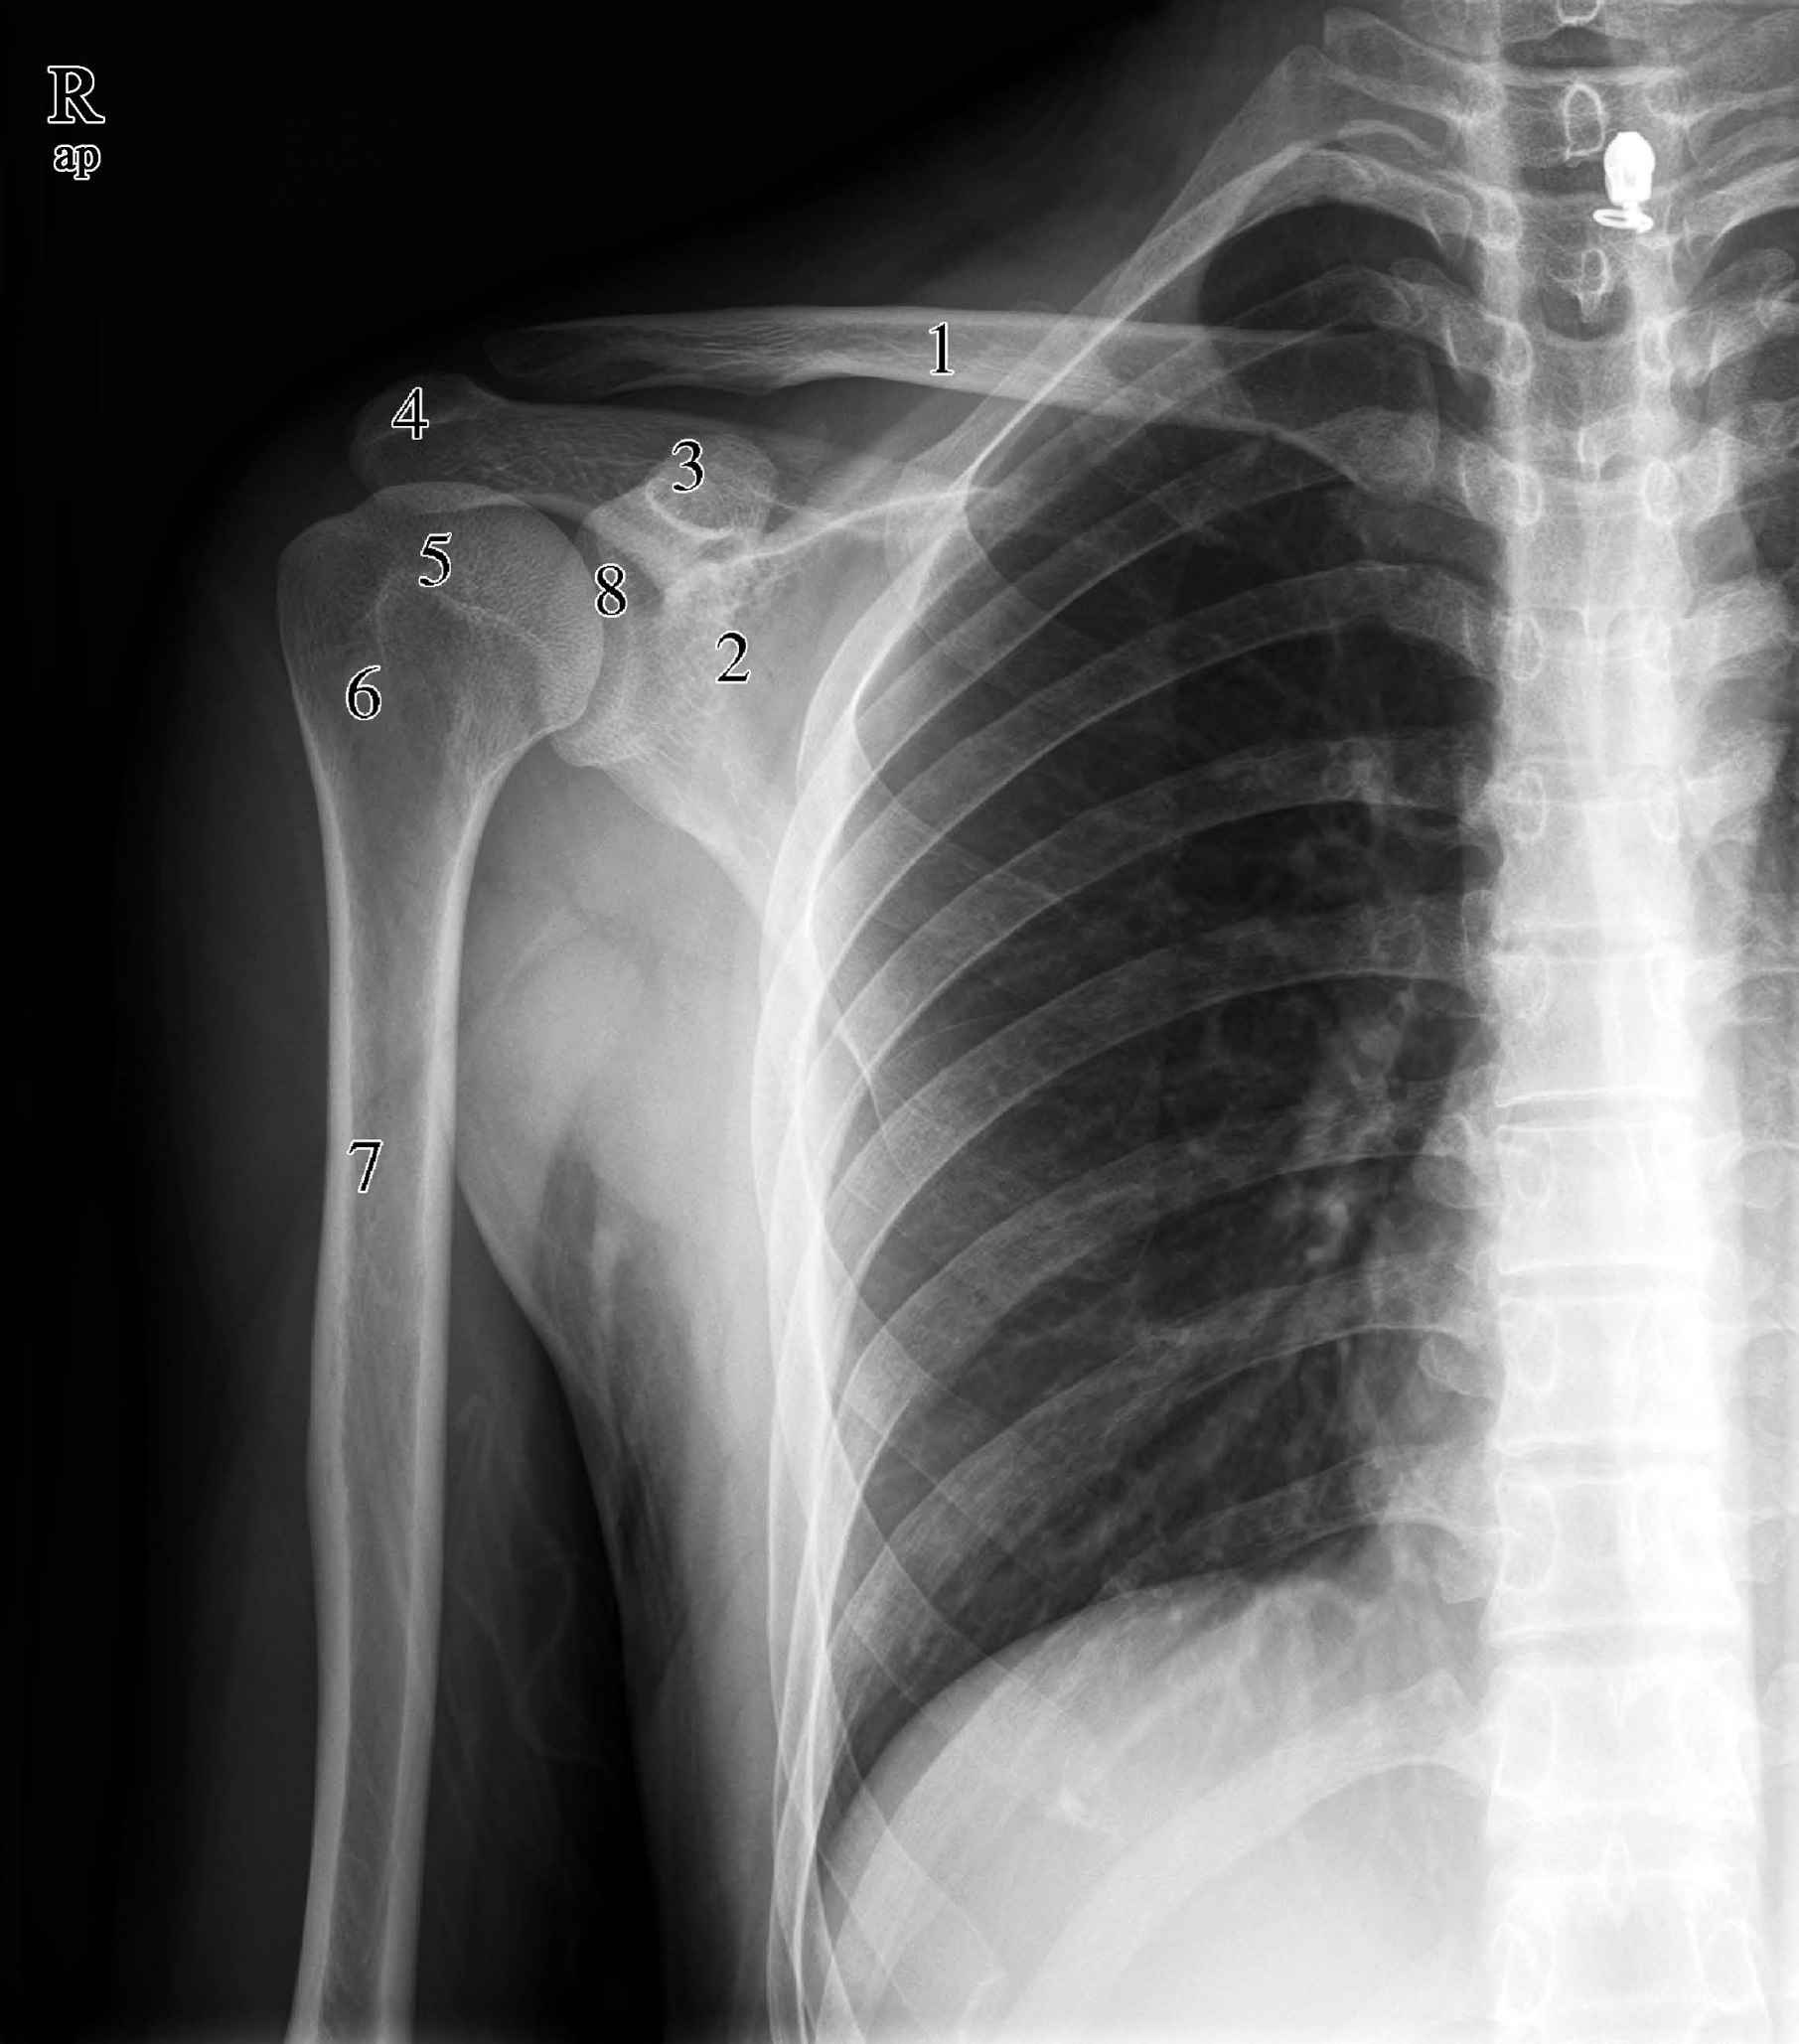
\includegraphics{./images/Image00003.jpg}
 \captionsetup{justification=centering}
 \caption{正常肩关节正位\\{\small 1.锁骨 2.肩胛骨 3.喙突 4.肩峰 5.肱骨头 6.肱骨外科颈 7.肱骨 8.肩关节盂}}
 \label{fig2-1-1}
  \end{figure} 

\textbf{【X线表现】}
 正常的肩关节由锁骨、肩胛骨和肱骨构成。锁骨呈横S形弯曲,内侧端粗而大,称胸骨端,有关节面与胸骨柄的锁切迹相关节,形成胸锁关节。外侧端扁平,称肩峰端。内侧2/3呈棱形,凸向前,外侧1/3呈扁平状,凸向后。肩胛骨为三角形扁骨分为关节盂、喙突、肩峰、体部和肩胛冈四部分。肩胛冈外侧端向前外侧的扁平突起,称肩峰,为肩部最高点;喙突从肩胛骨向上向内延伸,然后向前向外弯曲,位置较深,周围多为肌肉和韧带。肱骨为长管状骨,上端为肱骨头,与肩胛骨构成肩关节。肱骨骨干的上段为圆柱形,中段为三棱形,下段逐渐变为前后向的扁形。骨干的上端与肱骨大、小结节交界处略变细为肱骨外科颈,为骨折好发处。

\begin{figure}[!htbp]
 \centering
 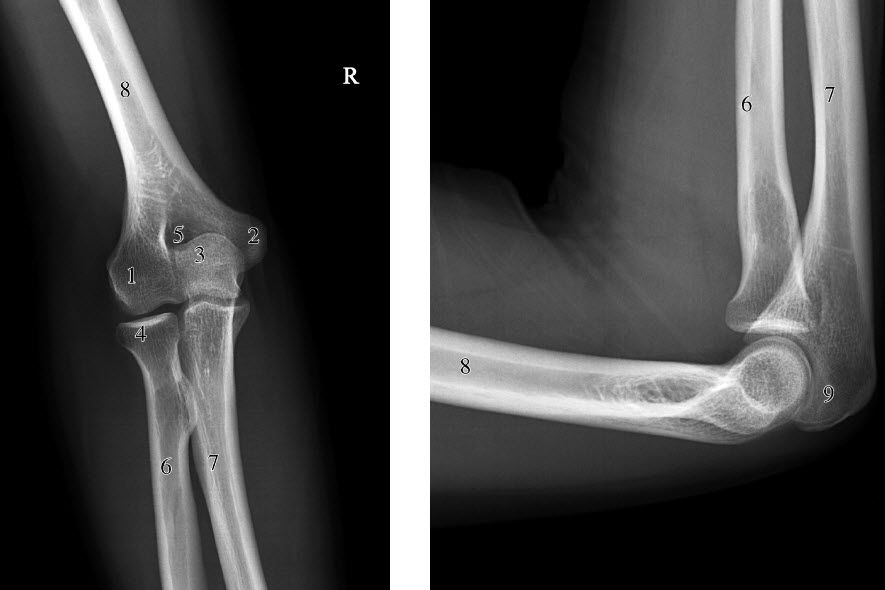
\includegraphics{./images/Image00004.jpg}
 \captionsetup{justification=centering}
 \caption{正常肘关节正侧位\\{\small 1.肱骨外上髁 2.肱骨内上髁 3.肱骨滑车 4.桡骨小头 5.鹰嘴窝 6.桡骨 7.尺骨 8.肱骨 9.尺骨鹰嘴}}
 \label{fig2-1-2}
  \end{figure} 

\textbf{【X线表现】}
 肘关节由肱、尺、桡三骨组成,由肱尺关节、肱桡关节与上尺桡关节共同组成的复合关节,且三个关节共同位于一个关节腔内,其骨性结构包括肱骨远端与尺骨、桡骨近端。肱骨远端内侧为肱骨滑车,内上为内上髁,外上为外上髁,滑车前方有冠状窝,后方有鹰嘴窝,两者之间仅有一层极薄的骨片相隔,所以髁上部易发生骨折。尺骨近端前方有冠状突,后方有鹰嘴,肱骨远端透光区为鹰嘴窝和冠状窝形成。桡骨近端为桡骨小头,小头下方为桡骨颈,桡骨颈内下方为桡骨粗隆。桡骨头无论在正位或是侧位始终对应肱骨小头,为关节在位。肱骨远端关节囊外有肘前及肘后脂肪垫,关节积液时被撑开形成八字征。

前臂骨由尺、桡骨组成,两骨之间有骨间膜,尺骨上大下小,桡骨上小下大。桡骨上端为桡骨小头,形如环状小盘,与肱骨小头构成关节,内侧还与尺骨的桡骨切迹形成上尺桡关节。尺骨远端为尺骨小头,与桡骨远端的尺骨切迹构成下尺桡关节,内侧尚有向下延伸的突起为尺骨茎突。桡骨远端膨大并形成关节面与腕部的手舟骨、月骨构成桡腕关节。其外侧有向下延伸的突起为桡骨茎突。

\begin{figure}[!htbp]
 \centering
 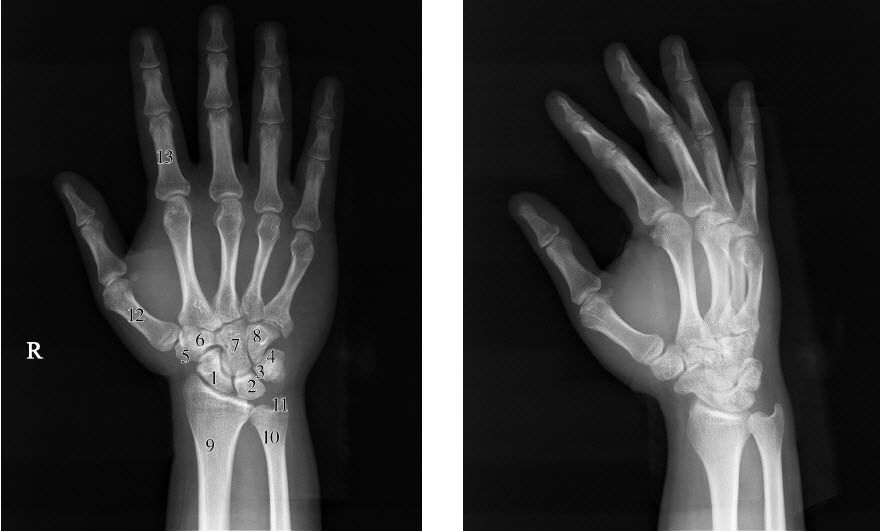
\includegraphics{./images/Image00005.jpg}
 \captionsetup{justification=centering}
 \caption{正常手腕关节正斜位\\{\small 1.手舟骨 2.月骨 3.三角骨 4.豆状骨 5.大多角骨 6.小多角骨 7.头状骨 8.钩状骨 9.桡骨 10.尺骨 11.尺骨茎突 12.第1掌骨 13.第2近节指骨}}
 \label{fig2-1-3}
  \end{figure} 

\textbf{【X线表现】}
 前臂与手的连接部位成为腕部,包括桡尺骨远端、8块腕骨和5个掌骨的近端,以及其相互构成的桡腕关节、腕骨间关节及腕掌关节。腕关节主要由桡骨远端和腕骨组成。尺骨远端因有三角软骨遮盖,故不与腕骨直接对应。尺桡骨远端关节面为凹形,与近排腕骨相对。腕关节的主要活动在桡腕关节。腕骨间的运动很少。腕部运动主要为背伸、掌屈、尺偏和桡偏。8块腕骨分两排,由外到内近排为手舟骨、月骨、三角骨、豆状骨(简称“舟月三角豆”),远排为大多角骨、小多角骨、头状骨、钩状骨(简称“大小头状钩”)。各骨相互形成腕间关节。近排的手舟骨、月骨和三角骨近端关节面与桡骨远端关节面共同构成桡腕关节。远排腕骨与各掌骨构成腕掌关节。

手部有5块掌骨和14块指骨,均为短管状骨,通过关节组成。掌骨和指骨近端为基底,中部为干,远端为头,远节指骨远端掌侧面粗糙,称为指骨粗隆。各关节由韧带及软组织相连。第2掌骨最长,第1掌骨最粗短。掌骨的近端与腕骨构成腕掌关节,远端分别与各指的近节指骨构成掌指关节。除了拇指只有两节指骨外,其余四指均有三节指骨,分别称为近节、中节和远节指骨。

\begin{figure}[!htbp]
 \centering
 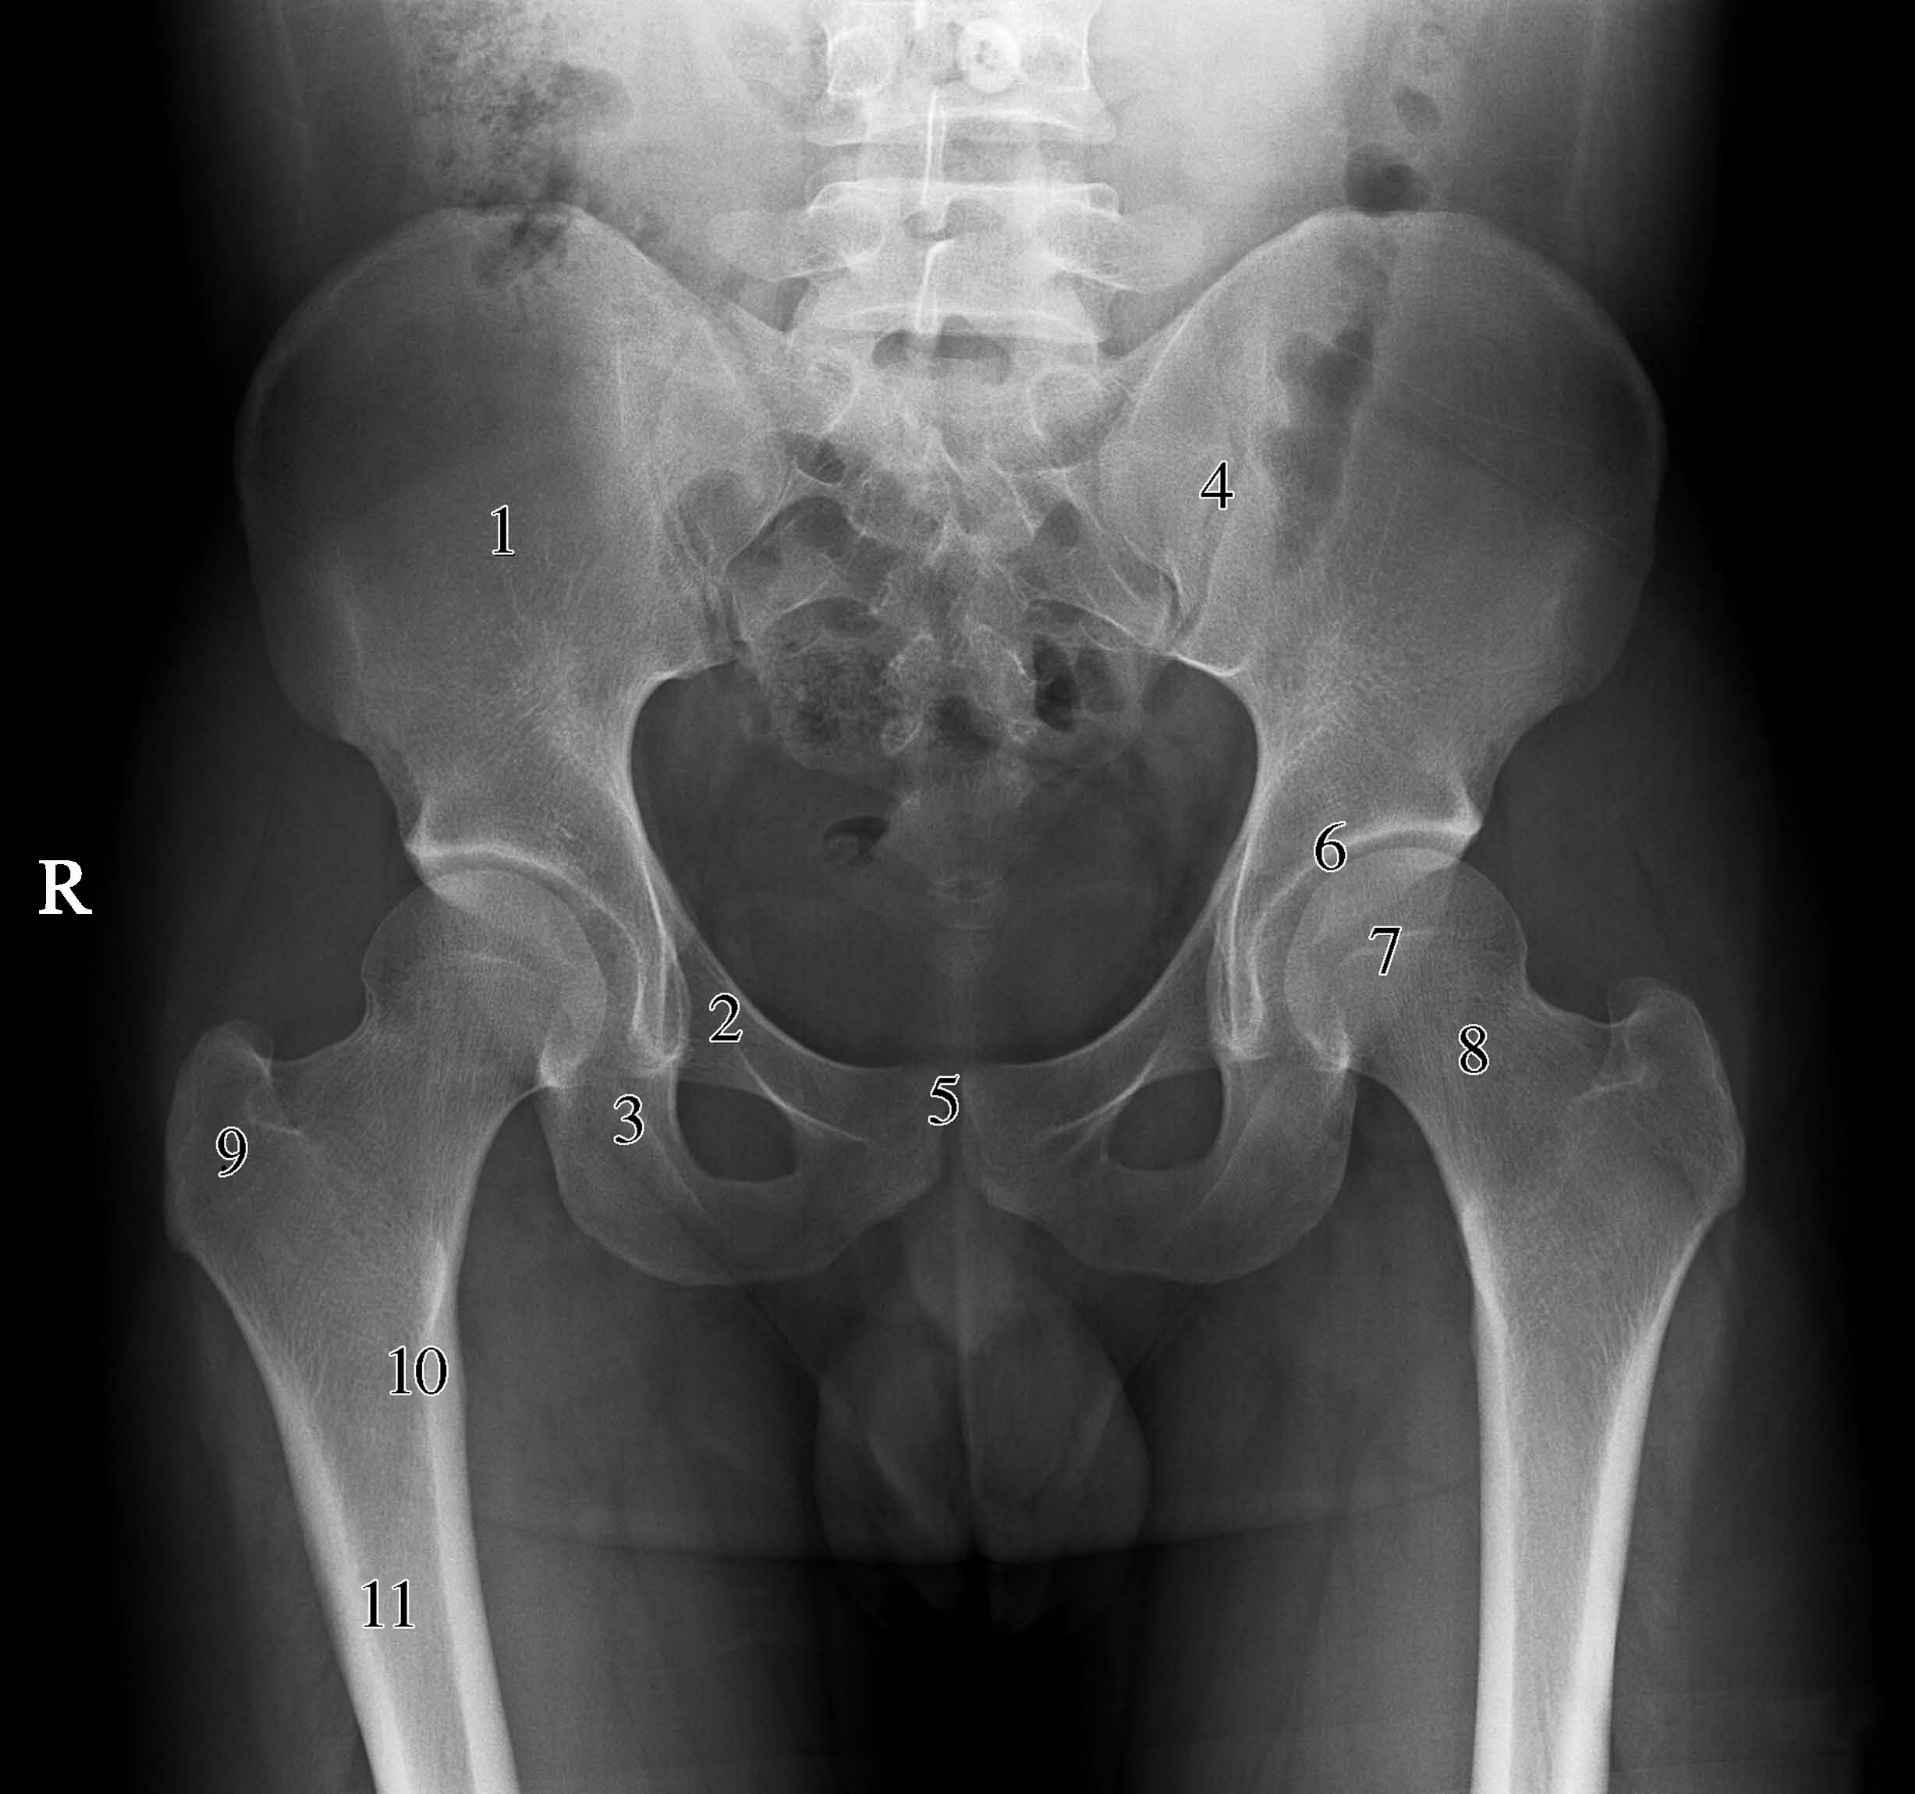
\includegraphics{./images/Image00006.jpg}
 \captionsetup{justification=centering}
 \caption{正常成人骨盆\\{\small 1.髂骨 2.耻骨上支 3.坐骨支 4.骶髂关节 5.耻骨联合 6.髋臼 7.股骨头 8.股骨颈 9.股骨大粗隆 10.股骨小粗隆 11.股骨干}}
 \label{fig2-1-4}
  \end{figure} 

\textbf{【X线表现】}
 骨盆由两侧的髋骨和后方的骶尾骨组成。髋骨上部为髂骨,前下部为耻骨,后下部为坐骨。两侧髂骨与骶骨构成骶髂关节。两侧耻骨由纤维软骨构成耻骨联合。髋关节由髋臼、股骨头及关节囊构成。髋臼口朝外下方,直径约3.5cm,窝内有半月形的关节面称月状面,髋臼中心对着小骨盆的髂耻线。髋臼后缘投影成一条致密线,横过股骨头。股骨头大部分套在髋臼之内,股骨头表面光滑,股骨颈的大部在髋关节囊内,股骨颈外上方为大粗隆,内下方偏后为小粗隆。

\begin{figure}[!htbp]
 \centering
 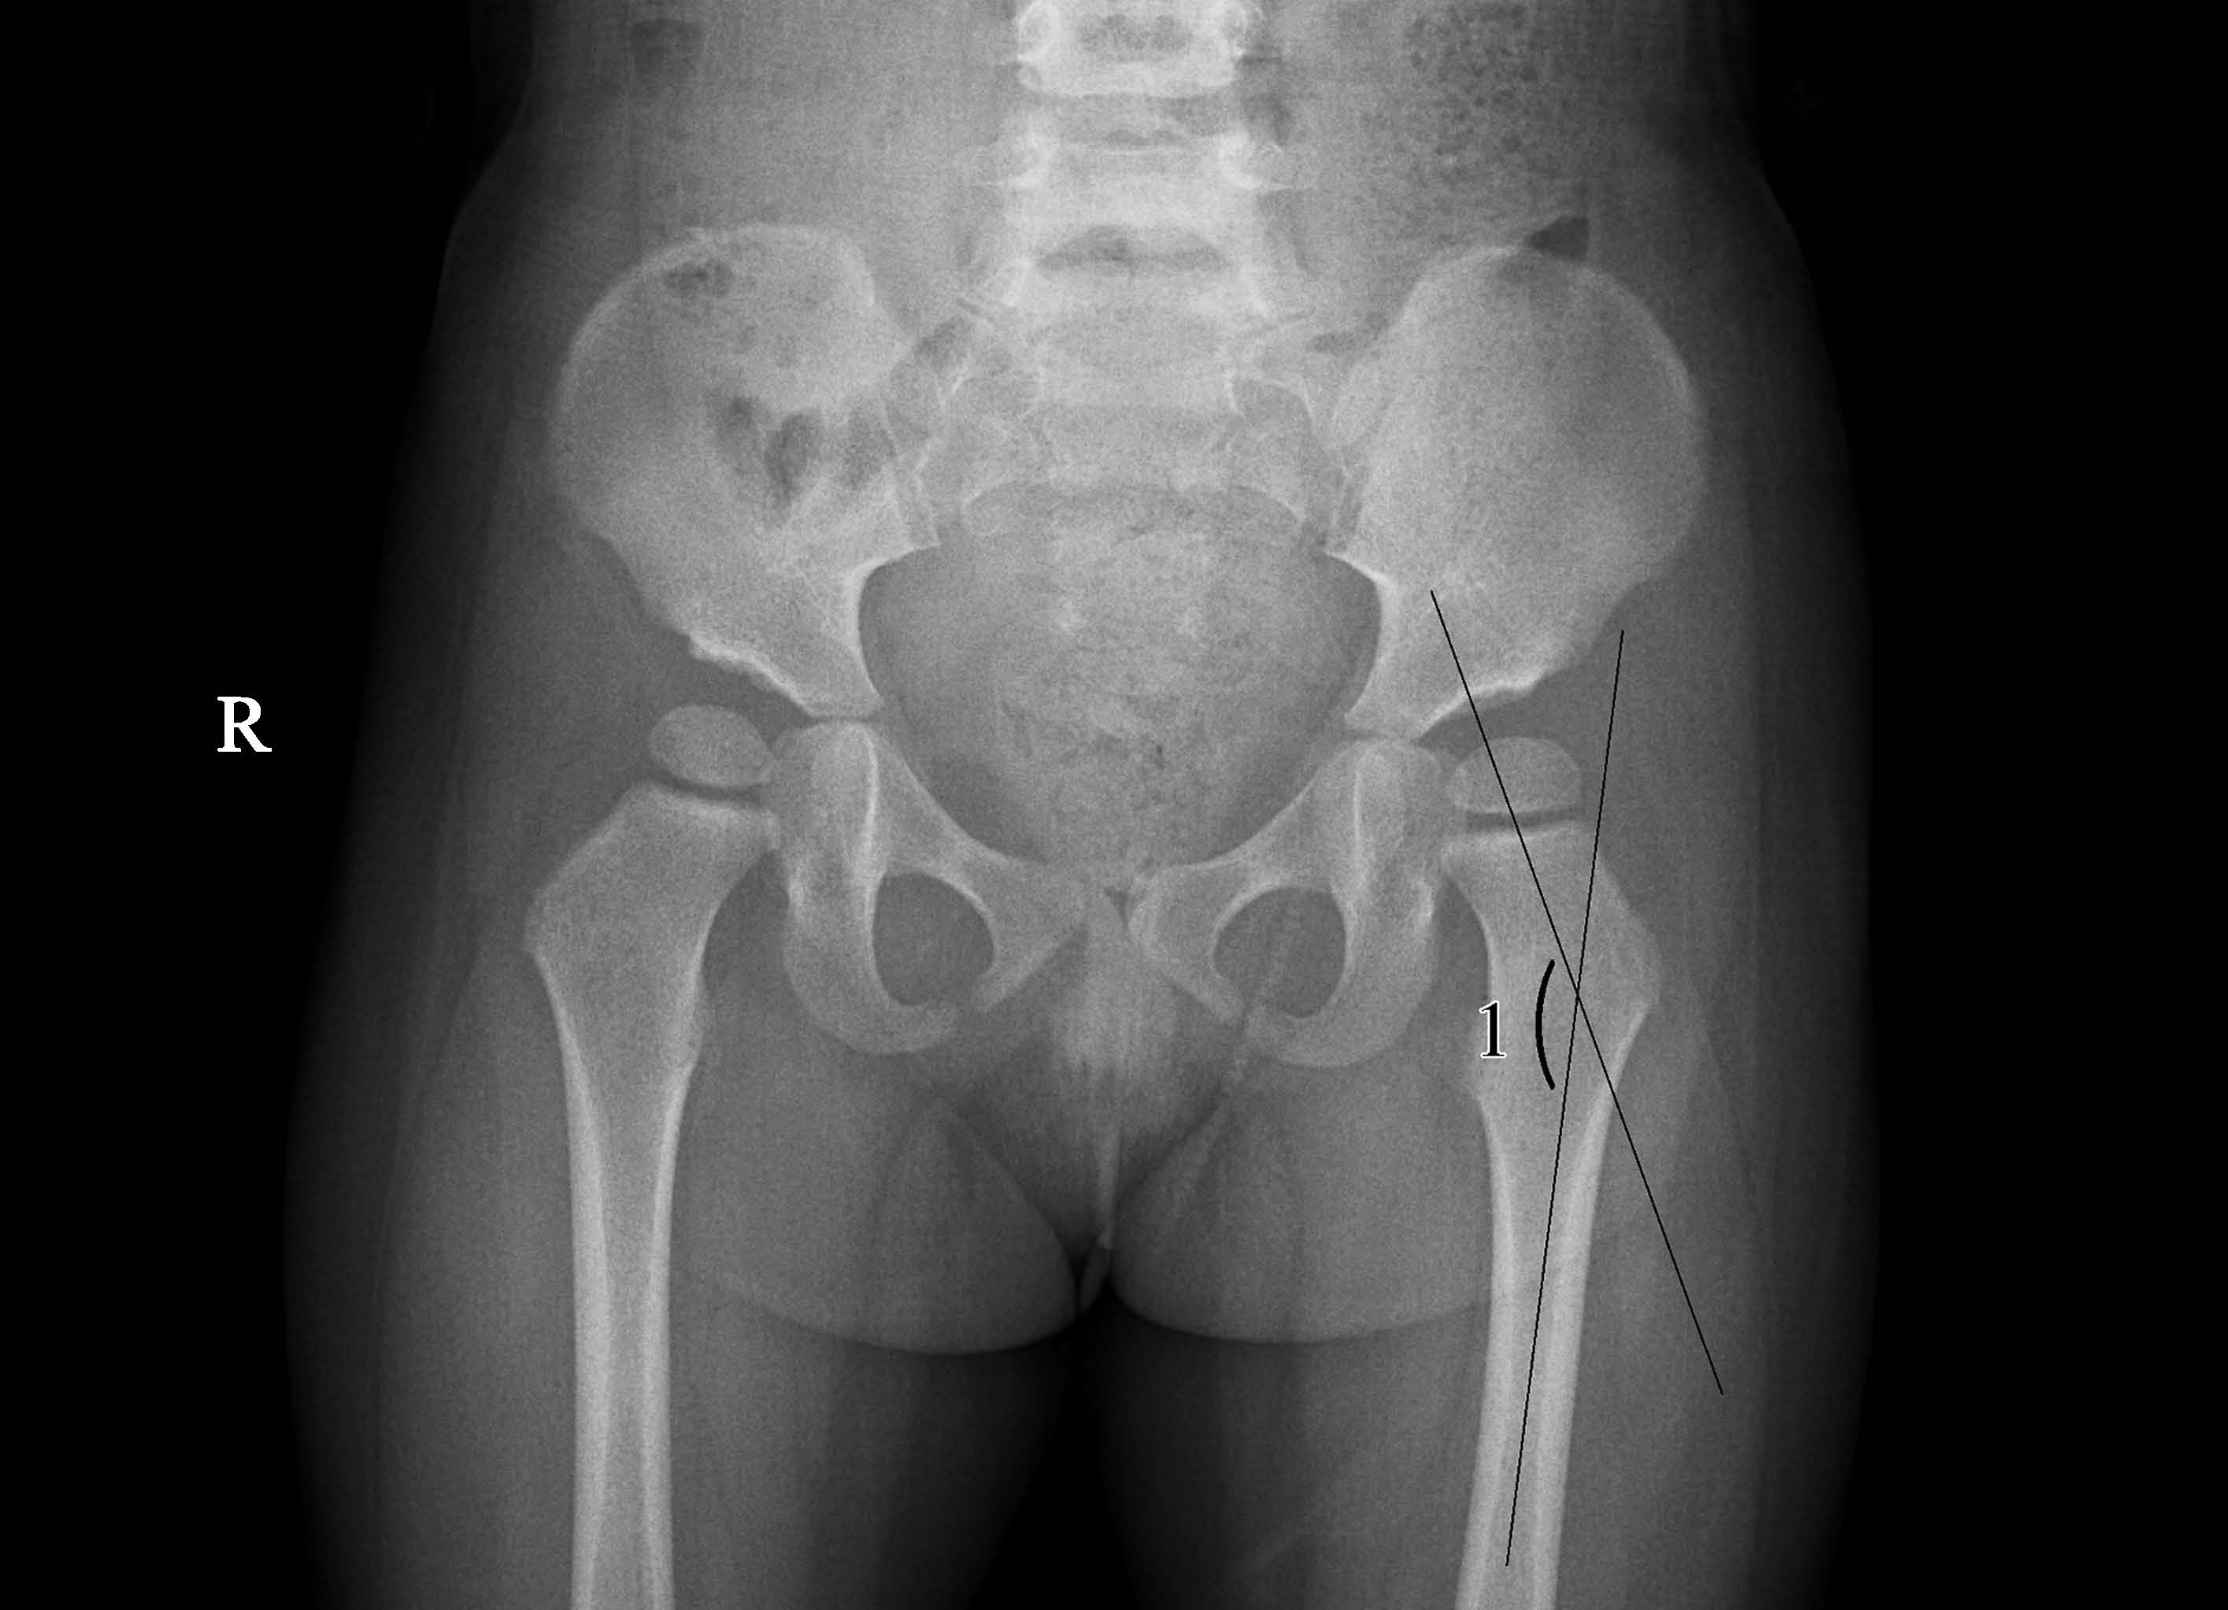
\includegraphics{./images/Image00007.jpg}
 \captionsetup{justification=centering}
 \caption{骨盆正位\\{\small 1.颈干角}}
 \label{fig2-1-5}
  \end{figure} 

\textbf{【X线表现】}
 股骨为人体内最长大、最结实的长骨。整个股骨呈圆柱形,骨干为长管状,略向内、后弯曲,其外层是较厚实的骨皮质,X线显示为均匀密实的高密度条形带状阴影,外缘锐利光滑,内缘不光滑。在骨干的中部,松质骨很少,而由脂肪及造血组织充填,称为骨髓腔。X线表现为模糊无结构的较透亮区。

(1)Y软骨连线:小儿的髋臼由髂骨、耻骨、坐骨组成,三者软骨连接点为Y软骨中心点,左右两点连一直线。正常时股骨头在此线的延长线下方。

(2)髋臼角:髋臼外上点与Y软骨顶点连一直线,再与Y软骨水平线向同侧的延长线相交之角,正常值30°~12°,随着年龄增长,角度缩小。

(3)申通线(Shenton's
line):闭孔上缘与同侧股骨颈画一弧线,若此线不存在为髋脱位。

(4)颈干角:股骨颈轴线与股骨干轴线相交之角,小儿130°,成人120°。

(5)Perkin方格象限:自髋臼外上点向下作垂直线与Y软骨的延长线相交形成四方格,正常股骨头位于内下象限内。

\begin{figure}[!htbp]
 \centering
 
\includegraphics{./images/Image00008.jpg}
 \captionsetup{justification=centering}
 \caption{正常膝关节正侧位\\{\small 1.股骨内上髁 2.股骨外上髁 3.髁间隆突 4.股骨 5.胫骨内侧髁 6.胫骨外侧髁 7.胫骨 8.腓骨 9.髌骨}}
 \label{fig2-1-6}
  \end{figure} 

\textbf{【X线表现】}
 膝关节由股骨远端、胫骨近端、髌骨组成,腓骨小头不参加膝关节的组成。股骨下端膨大部分形成内上髁、外上髁,其前端相连,与髌骨形成髌股关节。胫骨上端也分内侧髁和外侧髁,其平坦的关节面称为胫骨平台,中间为髁间隆突,可以限制膝关节的移动。胫骨外侧髁下方有小关节面,与腓骨小头形成上胫腓关节。胫骨上端前部的胫骨粗隆,是髌韧带的附着处。正位见股骨与胫骨关节面光整,关节间隙两侧对称,髌骨重叠于股骨远端,侧位见股骨、胫骨、髌骨形成关节。髌骨上方、股四头肌肌腱后方与股骨间形成髌上囊,其内含脂肪,X线下为透光影。髌骨下方、髌韧带后方,与股骨、胫骨间形成不等边四边形透光区,为髌下脂肪垫影。关节积液时此垫受压向前移位。

胫骨为长管状骨,骨干外侧与腓骨相邻缘有骨间嵴。腓骨为较细长的长管状骨,不承受体重,伴随于胫骨的外侧。骨干内侧与胫骨相邻缘亦有骨间嵴。上端略呈球形为腓骨头,其上突出的尖端称茎突。

\begin{figure}[!htbp]
 \centering
 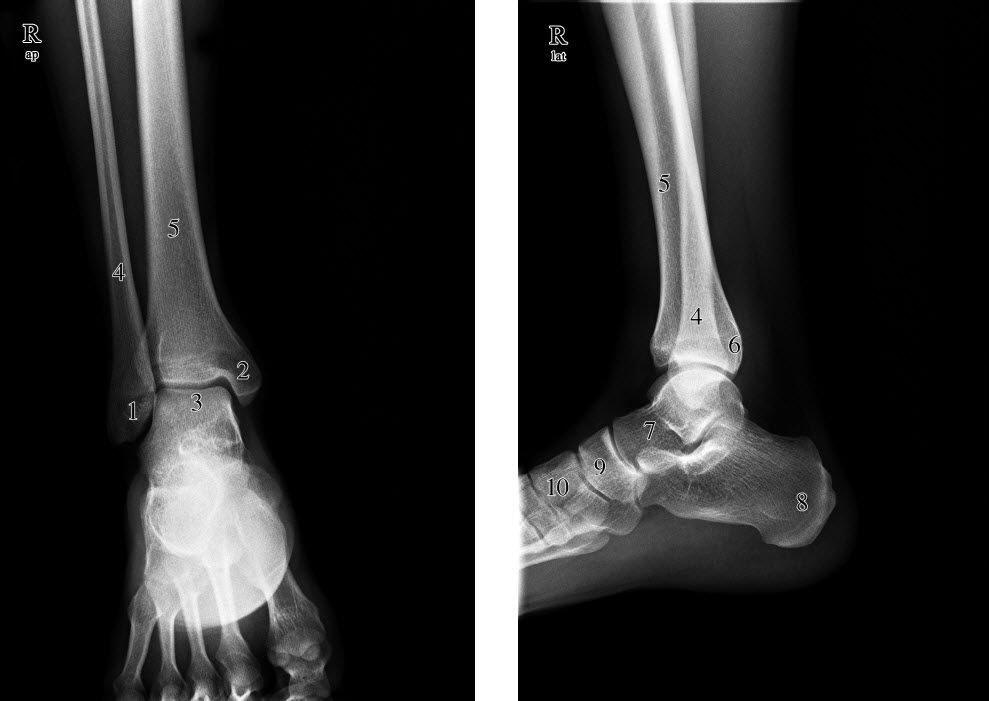
\includegraphics{./images/Image00009.jpg}
 \captionsetup{justification=centering}
 \caption{正常踝关节正侧位\\{\small 1.外踝 2.内踝 3.距骨滑车 4.腓骨 5.胫骨 6.后踝 7.距骨 8.跟骨 9.足舟骨 10.外侧楔状骨}}
 \label{fig2-1-7}
  \end{figure} 

\textbf{【X线表现】}
 踝关节由腓骨远端(外踝)、胫骨远端(内踝)、距骨滑车组成,胫骨下端内侧为内踝,腓骨下端为外踝,胫骨前方为前踝,胫骨后方为后踝,胫骨的腓骨切迹与腓骨下部组成胫腓联合关节。诸关节间隙清晰光整。踝关节前后关节囊均可见囊外脂肪层。

\begin{figure}[!htbp]
 \centering
 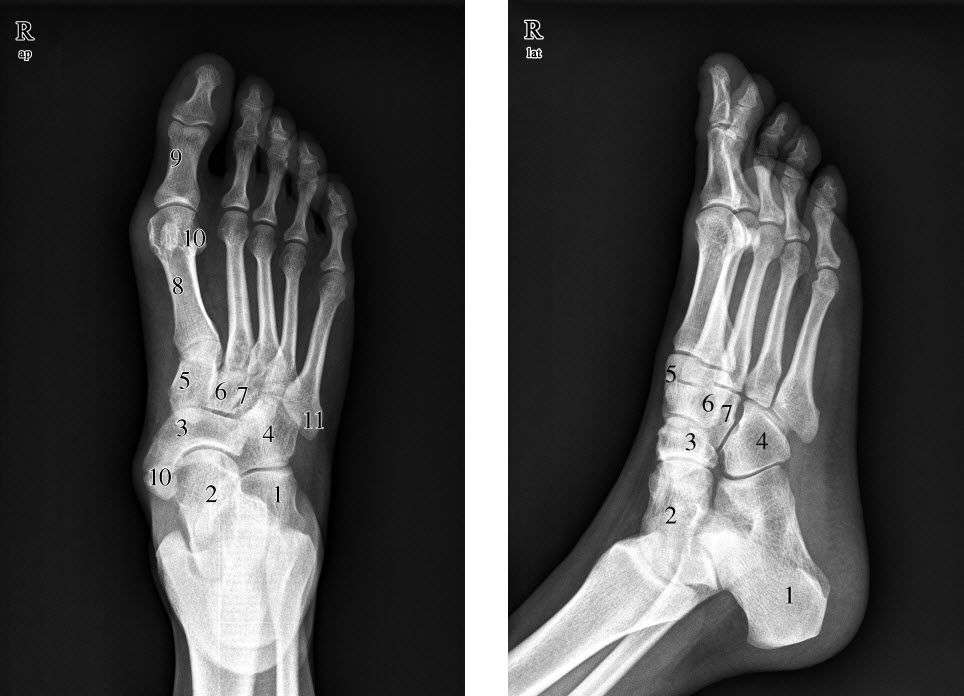
\includegraphics{./images/Image00010.jpg}
 \captionsetup{justification=centering}
 \caption{正常足正斜位\\{\small 1.跟骨 2.距骨 3.足舟骨 4.骰骨 5.内侧楔状骨 6.中间楔状骨 7.外侧楔状骨 8.第1跖骨 9.第1近节趾骨 10.籽骨 11.第5跖骨粗隆}}
 \label{fig2-1-8}
  \end{figure} 

\textbf{【X线表现】}
 足部骨骼包括趾骨、跖骨和跗骨。跟骨呈弓形,可分为体部和跟结节。每侧足共有14个趾骨:其中第1趾2节,其余各趾各有3节。跖骨共有5块:第1跖骨最粗短,第2跖骨最长。跗骨共有7块:分别为跟骨、距骨、舟骨、骰骨及内侧楔骨、中间楔骨、外侧楔骨。在第1跖骨远端常可见小籽骨,在足舟骨的内侧亦可见一籽骨(副舟骨)。

\begin{figure}[!htbp]
 \centering
 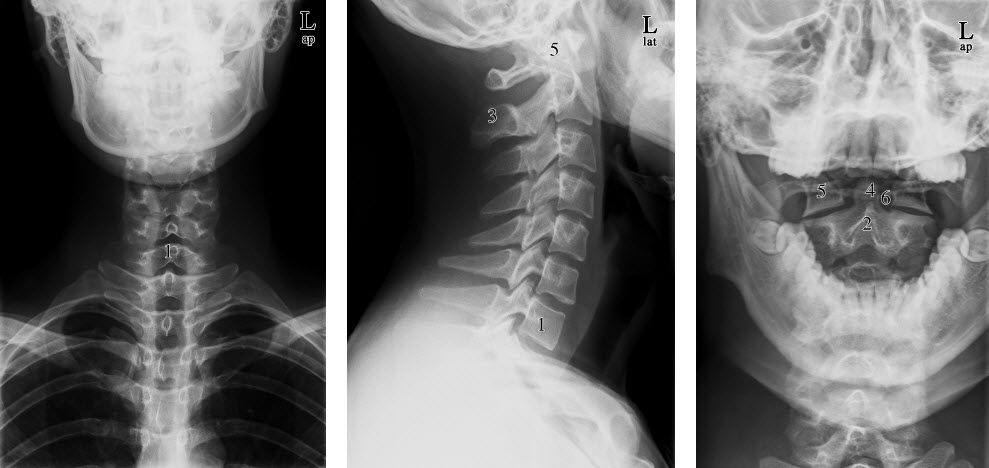
\includegraphics{./images/Image00011.jpg}
 \captionsetup{justification=centering}
 \caption{颈椎正侧位;张口位\\{\small 1.第7颈椎椎体 2.枢椎椎体 3.寰椎棘突 4.齿状突 5.寰椎侧块 6.寰枢关节}}
 \label{fig2-1-9}
  \end{figure} 

\textbf{【X线表现】}
 寰椎无椎体,由两个侧块将前后弓联合。枢椎椎体前上部有一齿状突起,称齿状突,齿状突与寰椎前弓后缘构成关节。枢椎的齿状突与寰椎侧块间距离,正常两侧应相等。

第3~7颈椎椎体在正位上呈鞍形,椎体上缘两侧端可见斜面向内的三角形突起称为钩突,侧位上可见第2颈椎棘突又宽又大、第7颈椎棘突最长。颈椎侧位平片的重点:①7个椎体清晰可辨;②椎前间隙存在;③4条平行弧线分别连续下降(椎体前线、椎体后线、棘突椎板线和棘后线);④寰齿间距;⑤椎间隙(增宽或变窄)。

\begin{figure}[!htbp]
 \centering
 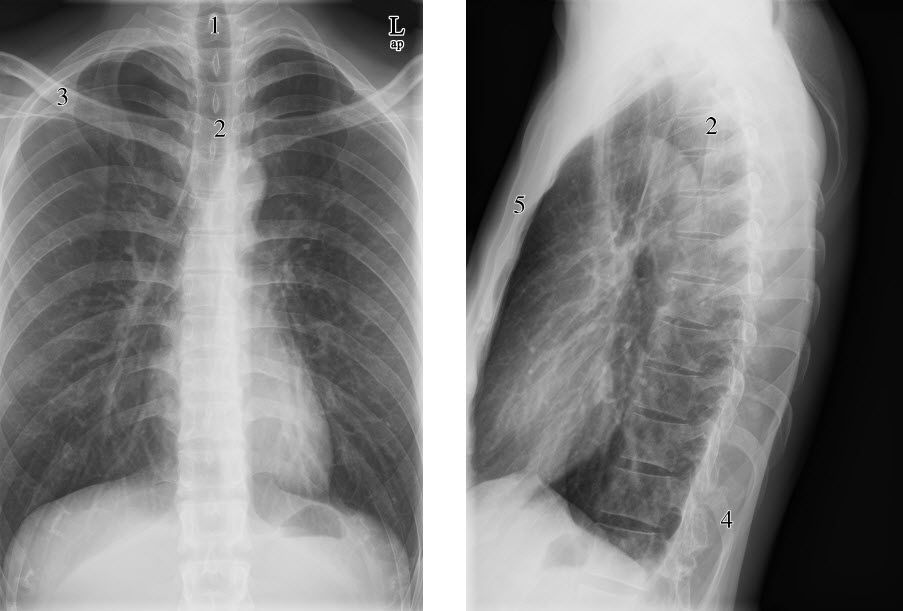
\includegraphics{./images/Image00012.jpg}
 \captionsetup{justification=centering}
 \caption{胸椎正侧位\\{\small 1.第1胸椎椎体 2.第4胸椎椎体 3.锁骨 4.第12后肋 5.胸骨}}
 \label{fig2-1-10}
  \end{figure} 

\textbf{【X线表现】}
 正常胸椎由12个椎体构成,椎体形态较规则,呈四方形。椎间隙因生理性前曲的关系在侧位上显示前窄后宽。椎间小关节的关节面呈冠状位,故关节间隙需在侧位片显示,椎间孔亦在侧位片上显示。每根肋骨的肋小头与胸椎椎体的肋凹构成肋椎关节,同时肋结节和横突肋凹构成肋横突关节(第11肋、第12肋无此关节)。

目前比较一致公认的脊柱三柱分类概念为:脊柱分为前柱、中柱、后柱三柱,脊柱的稳定性有赖于中柱的完整。其中前柱为前纵韧带、椎体和椎间盘的前2/3;中柱为后纵韧带、椎体和椎间盘的后1/3部;后柱为椎弓、黄韧带、棘间韧带。凡中柱损伤者属于不稳定性骨折。

\begin{figure}[!htbp]
 \centering
 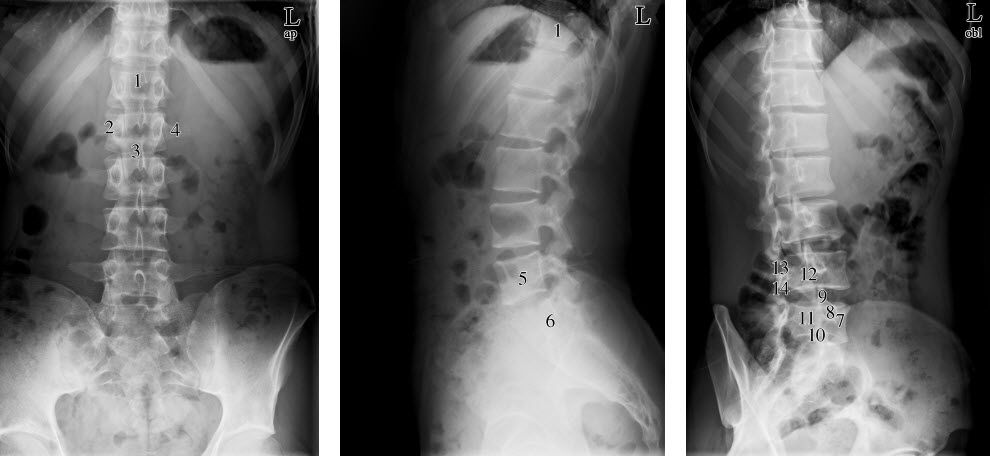
\includegraphics{./images/Image00013.jpg}
 \captionsetup{justification=centering}
 \caption{正常腰椎正侧位、斜位\\{\small 1.第1腰椎椎体 2.第2腰椎椎弓根 3.第2腰椎棘突 4.第2腰椎左侧横突 5.第5腰椎 6.第1骶椎 7.近片侧横突 8.椎弓根 9.上关节突 10.下关节突 11.椎板 12.椎弓峡部 13.远片侧横突 14.远片侧下关节突}}
 \label{fig2-1-11}
  \end{figure} 

\textbf{【X线表现】}
 腰椎椎体形态较粗大,近似四方形。椎间隙因生理性后曲的关系在侧位上显示为前宽后窄。椎间小关节的关节面多呈矢状位,故关节间隙在正位片显示良好。椎间孔在侧位片上显示。斜位片上椎弓形态类似狗的模样:近片侧横突相当于狗嘴,椎弓根为狗眼,上关节突相当于狗耳,下关节突是狗前腿,狗耳与狗前腿间的间隙为近侧的小关节间隙,椎板相当于狗腹,峡部相当于狗颈;远片侧横突相当于狗尾,下关节突相当于狗后腿。

\begin{figure}[!htbp]
 \centering
 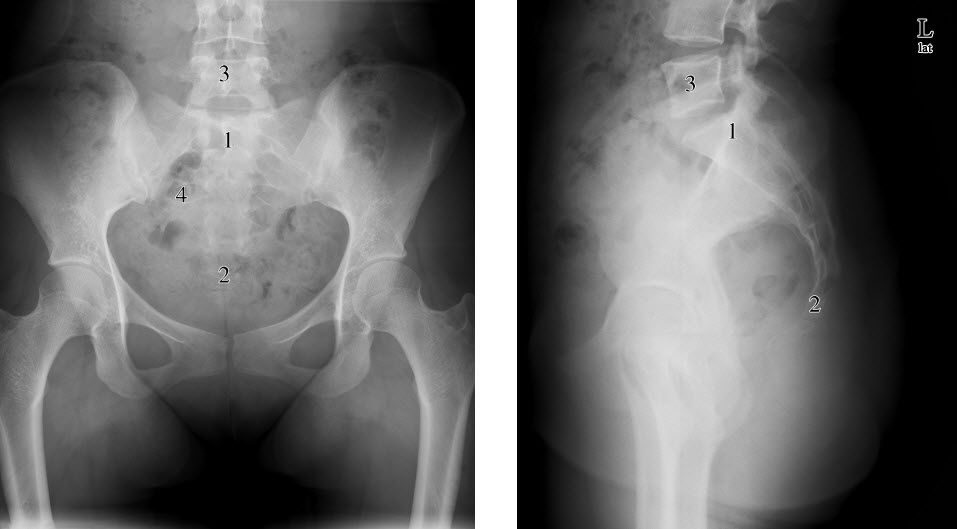
\includegraphics{./images/Image00014.jpg}
 \captionsetup{justification=centering}
 \caption{骶尾椎正侧位\\{\small 1.第1骶椎椎体 2.第1尾椎 3.第5腰椎椎体 4.骶前孔}}
 \label{fig2-1-12}
  \end{figure} 

\textbf{【X线表现】}
 骶骨由5节骶椎融合而成,呈倒三角形,底向上,尖向下,前面凹陷,上缘中分向前隆突称岬,中部有4条横线,横线两端有4对骶前孔。背面粗糙隆突,正中部为骶正中嵴,中间部为骶中间嵴,此嵴外侧有4对骶后孔,孔外侧部有骶外侧嵴。骶前后孔与骶管相通,有骶神经前、后支通过。骶管下端的裂孔为骶管裂孔,两侧向下突出为骶角。骶骨外侧部上份有耳状面,与髋骨耳状面相关节,为骨盆的后壁。上与第5腰椎相连,下与尾骨相连。尾骨由3~4节退化的尾椎融合而成。骶尾骨共同形成向后的生理弯曲。

\begin{figure}[!htbp]
 \centering
 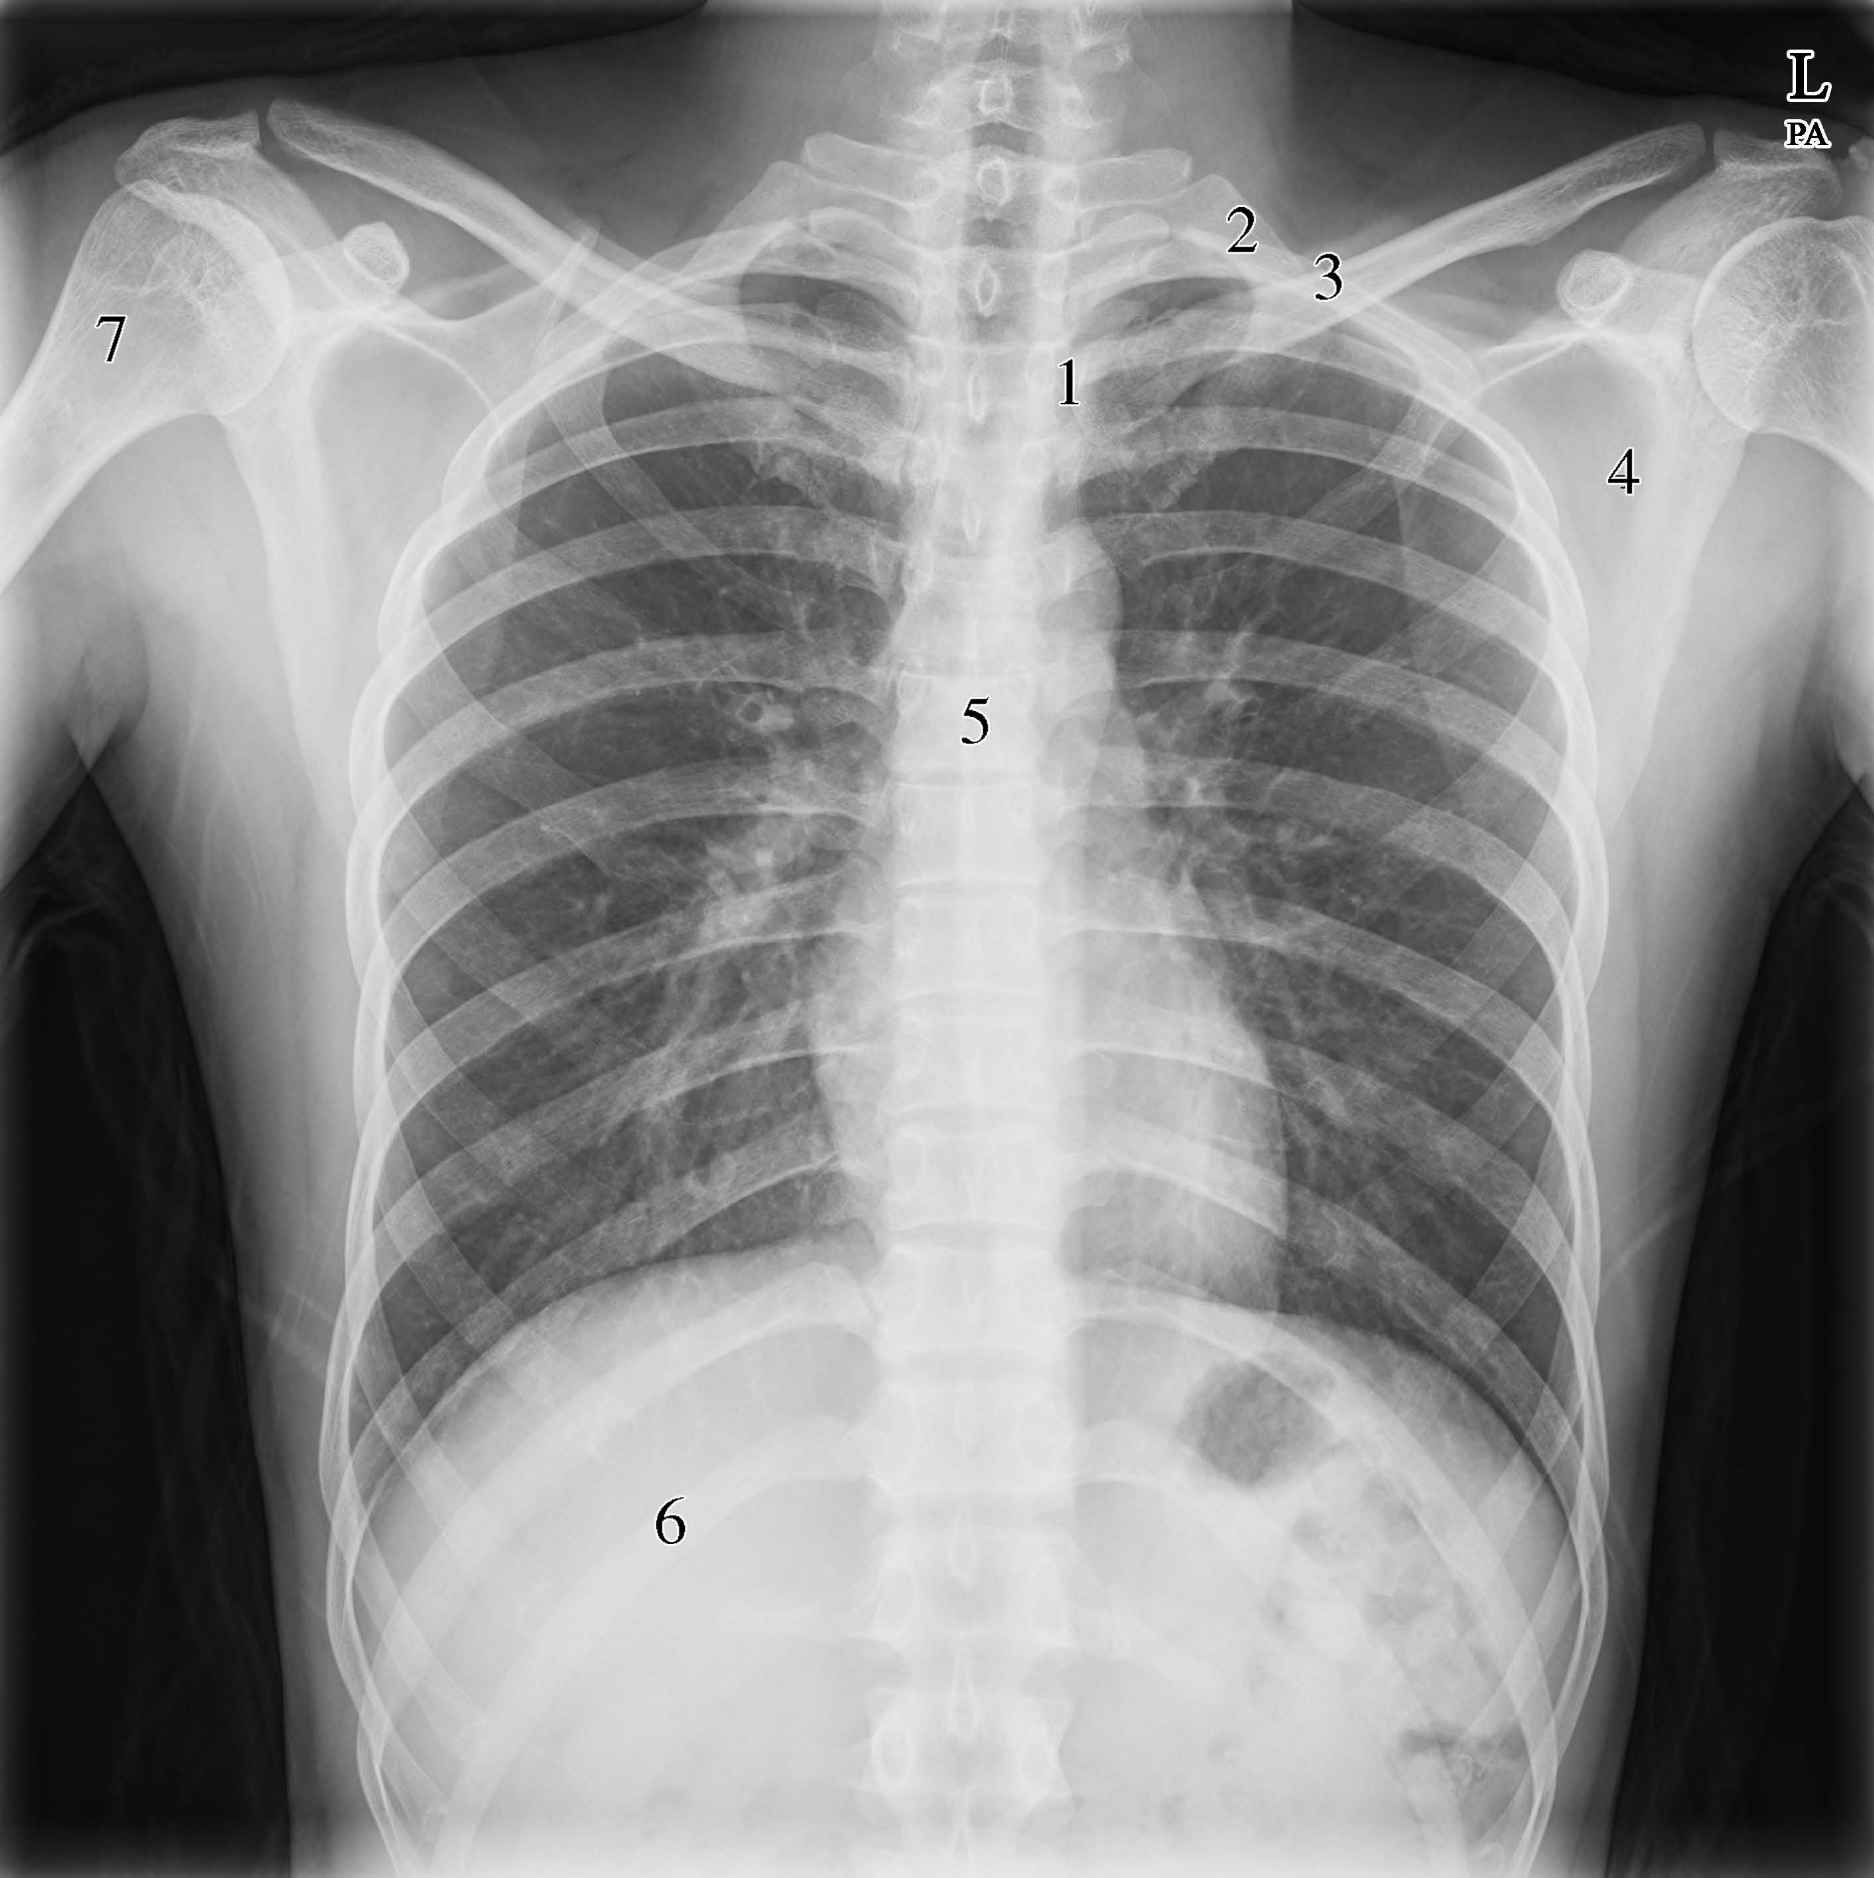
\includegraphics{./images/Image00015.jpg}
 \captionsetup{justification=centering}
 \caption{正常肋骨正位\\{\small 1.左侧胸锁关节 2.左侧第1肋骨 3.锁骨 4.肩胛骨 5.第6胸椎椎体 6.右侧第12浮肋 7.肱骨}}
 \label{fig2-1-13}
  \end{figure} 

\textbf{【X线表现】}
 胸廓由12个胸椎、12对肋骨和胸骨借关节和软骨连结而组成。肋骨12对,左右对称,后端与胸椎相关节;前端仅第1~7肋借软骨与胸骨相连结,形成肋弓,第11、12肋骨前端游离,又称浮肋。胸骨位于胸前壁正中,分柄、体、剑突三部分。构成胸廓的主要关节有胸锁关节、胸肋关节和肋椎关节。

\begin{figure}[!htbp]
 \centering
 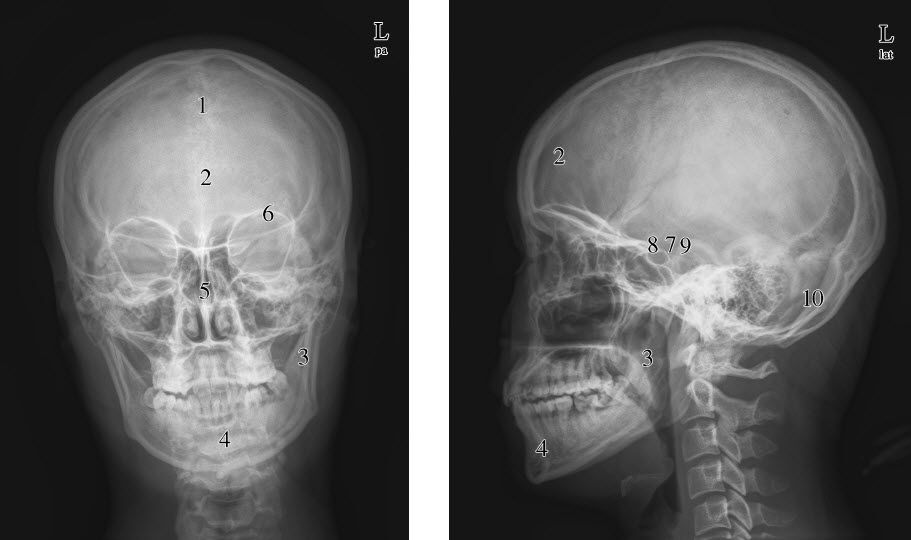
\includegraphics{./images/Image00016.jpg}
 \captionsetup{justification=centering}
 \caption{颅面骨正侧位\\{\small 1.矢状缝 2.额骨 3.下颌支 4.下颌骨体部 5.鼻中隔 6.左侧眼眶 7.蝶鞍 8.前床突 9.后床突 10.枕骨}}
 \label{fig2-1-14}
  \end{figure} 

\textbf{【X线表现】}
 颅骨分颅盖骨和颅底骨两部分,前者由额骨、顶骨、颞骨及枕骨组成,后者由蝶骨、岩骨、筛骨、额骨眶板和枕骨等组成,各颅骨均包括颅骨内外板和板障。

颅缝为两块颅骨衔接处,呈锯齿状。额、顶骨间为冠状缝,顶、枕骨间为人字缝,都可在侧位片中显示清楚。颞、顶骨间为鳞状缝(或称颞鳞缝),侧位片中能见度较差,两顶骨间为前后走向的矢状缝。颅缝间多余的骨块,为缝间骨,多见于人字缝,不可误认为骨折。颅缝宽度不超过2mm,随年龄增长而逐渐变窄。冠状缝、人字缝和矢字缝约30岁闭合。

蝶鞍是观察头颅平片的重点。因它位于颅底部的中央,无论鞍内、蝶鞍附近或离其较远的颅内占位病变常直接地或间接地影响蝶鞍,并引起相应的骨质改变。其形状有椭圆形、圆形和扁平形三种。成人大多为椭圆形,小儿以圆形占多数。其前后壁间最大距离为前后径,为8~16mm(平均11.5mm);前后床突间连线至鞍底间最大垂直距离为深径,为7~14mm(平均9.5mm)。蝶鞍前方以鞍结节及向下延续的前壁为界,鞍结节两侧的蝶骨小翼对称地向内后方的骨性隆起为前床突。鞍背为蝶鞍后界,其前缘的外上角有后床突指向外方。蝶鞍与其下方的蝶窦隔以鞍底。鞍底为一薄层密质骨,轮廓清楚,侧位片中平直或轻度凹陷。

\section{骨、关节先天发育畸形}

\subsection{融合椎}

\begin{figure}[!htbp]
 \centering
 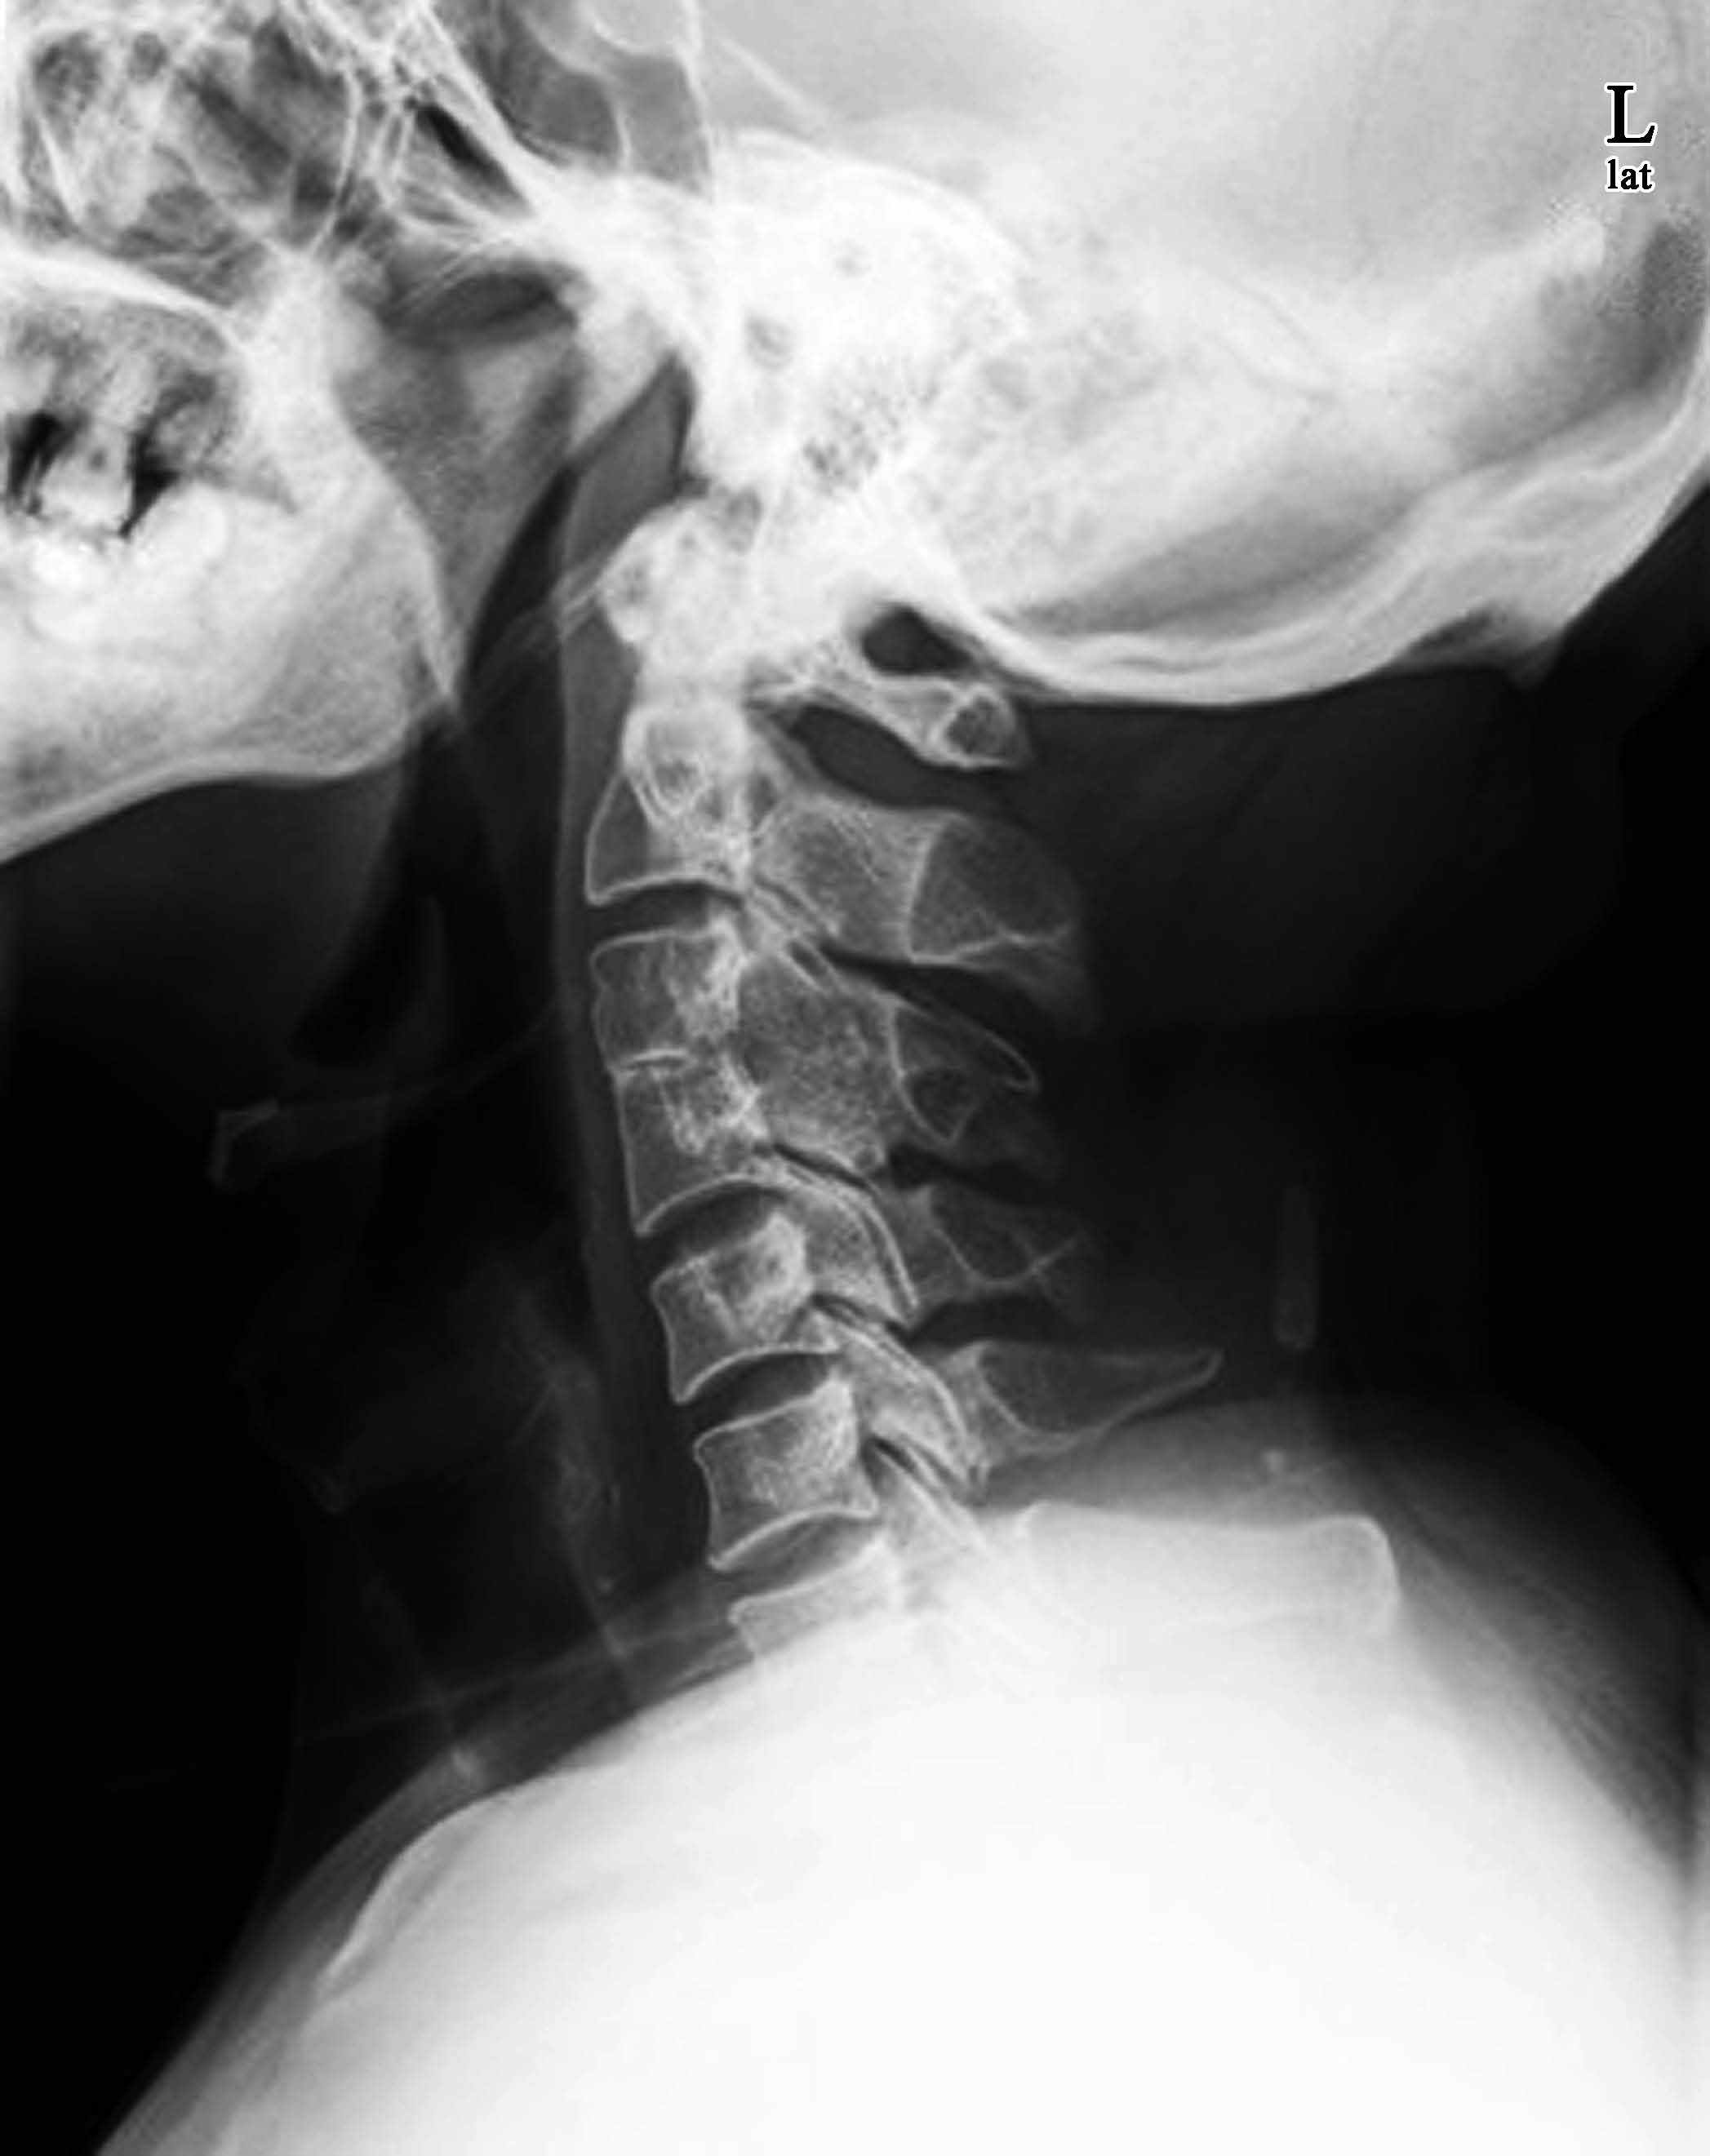
\includegraphics{./images/Image00017.jpg}
 \captionsetup{justification=centering}
 \caption{颈椎侧位}
 \label{fig2-2-1}
  \end{figure} 

\textbf{【病史摘要】}  男性,53岁。体检时发现C3、C4椎体融合。

\textbf{【X线表现】}  C3、C4椎体、棘突骨性融合。

\textbf{【X线诊断】}  C3、C4融合椎。

\textbf{【评  述】}
 本病由于脊柱分节异常导致邻近的两个或多个椎体完全或部分互相融合。有时椎弓、椎板、小关节甚至棘突也融合在一起。常见于腰椎,其次为颈椎,胸椎较少。如发生在胸椎,相邻的肋骨也可受累。需要与病理性融合椎鉴别。先天性融合椎,表现为融合在一起的椎体,其总高度与相邻单个椎体高度之和相仿;而病理性融合椎,表现为融合椎的总高度低于相邻单个椎体高度之和。

颈椎融合综合征系颈椎两节以上的先天性融合又称Klippel-Feil综合征(K-F综合征)、短颈综合征、颈胸椎体先天性骨结合综合征等。临床以颈椎缩短、后发际低和颈部活动受限等三联征为特征。短颈畸形可合并颈肋、隐性脊柱裂、神经根或神经丛分布畸形,可出现臂痛、腰痛和坐骨神经痛。合并心脏畸形、肾脏畸形者也会出现相应的临床症状。此外,短颈畸形也可合并脊柱侧弯、高位肩胛骨和蹼状畸形等。

\subsection{裂椎畸形}

\begin{figure}[!htbp]
 \centering
 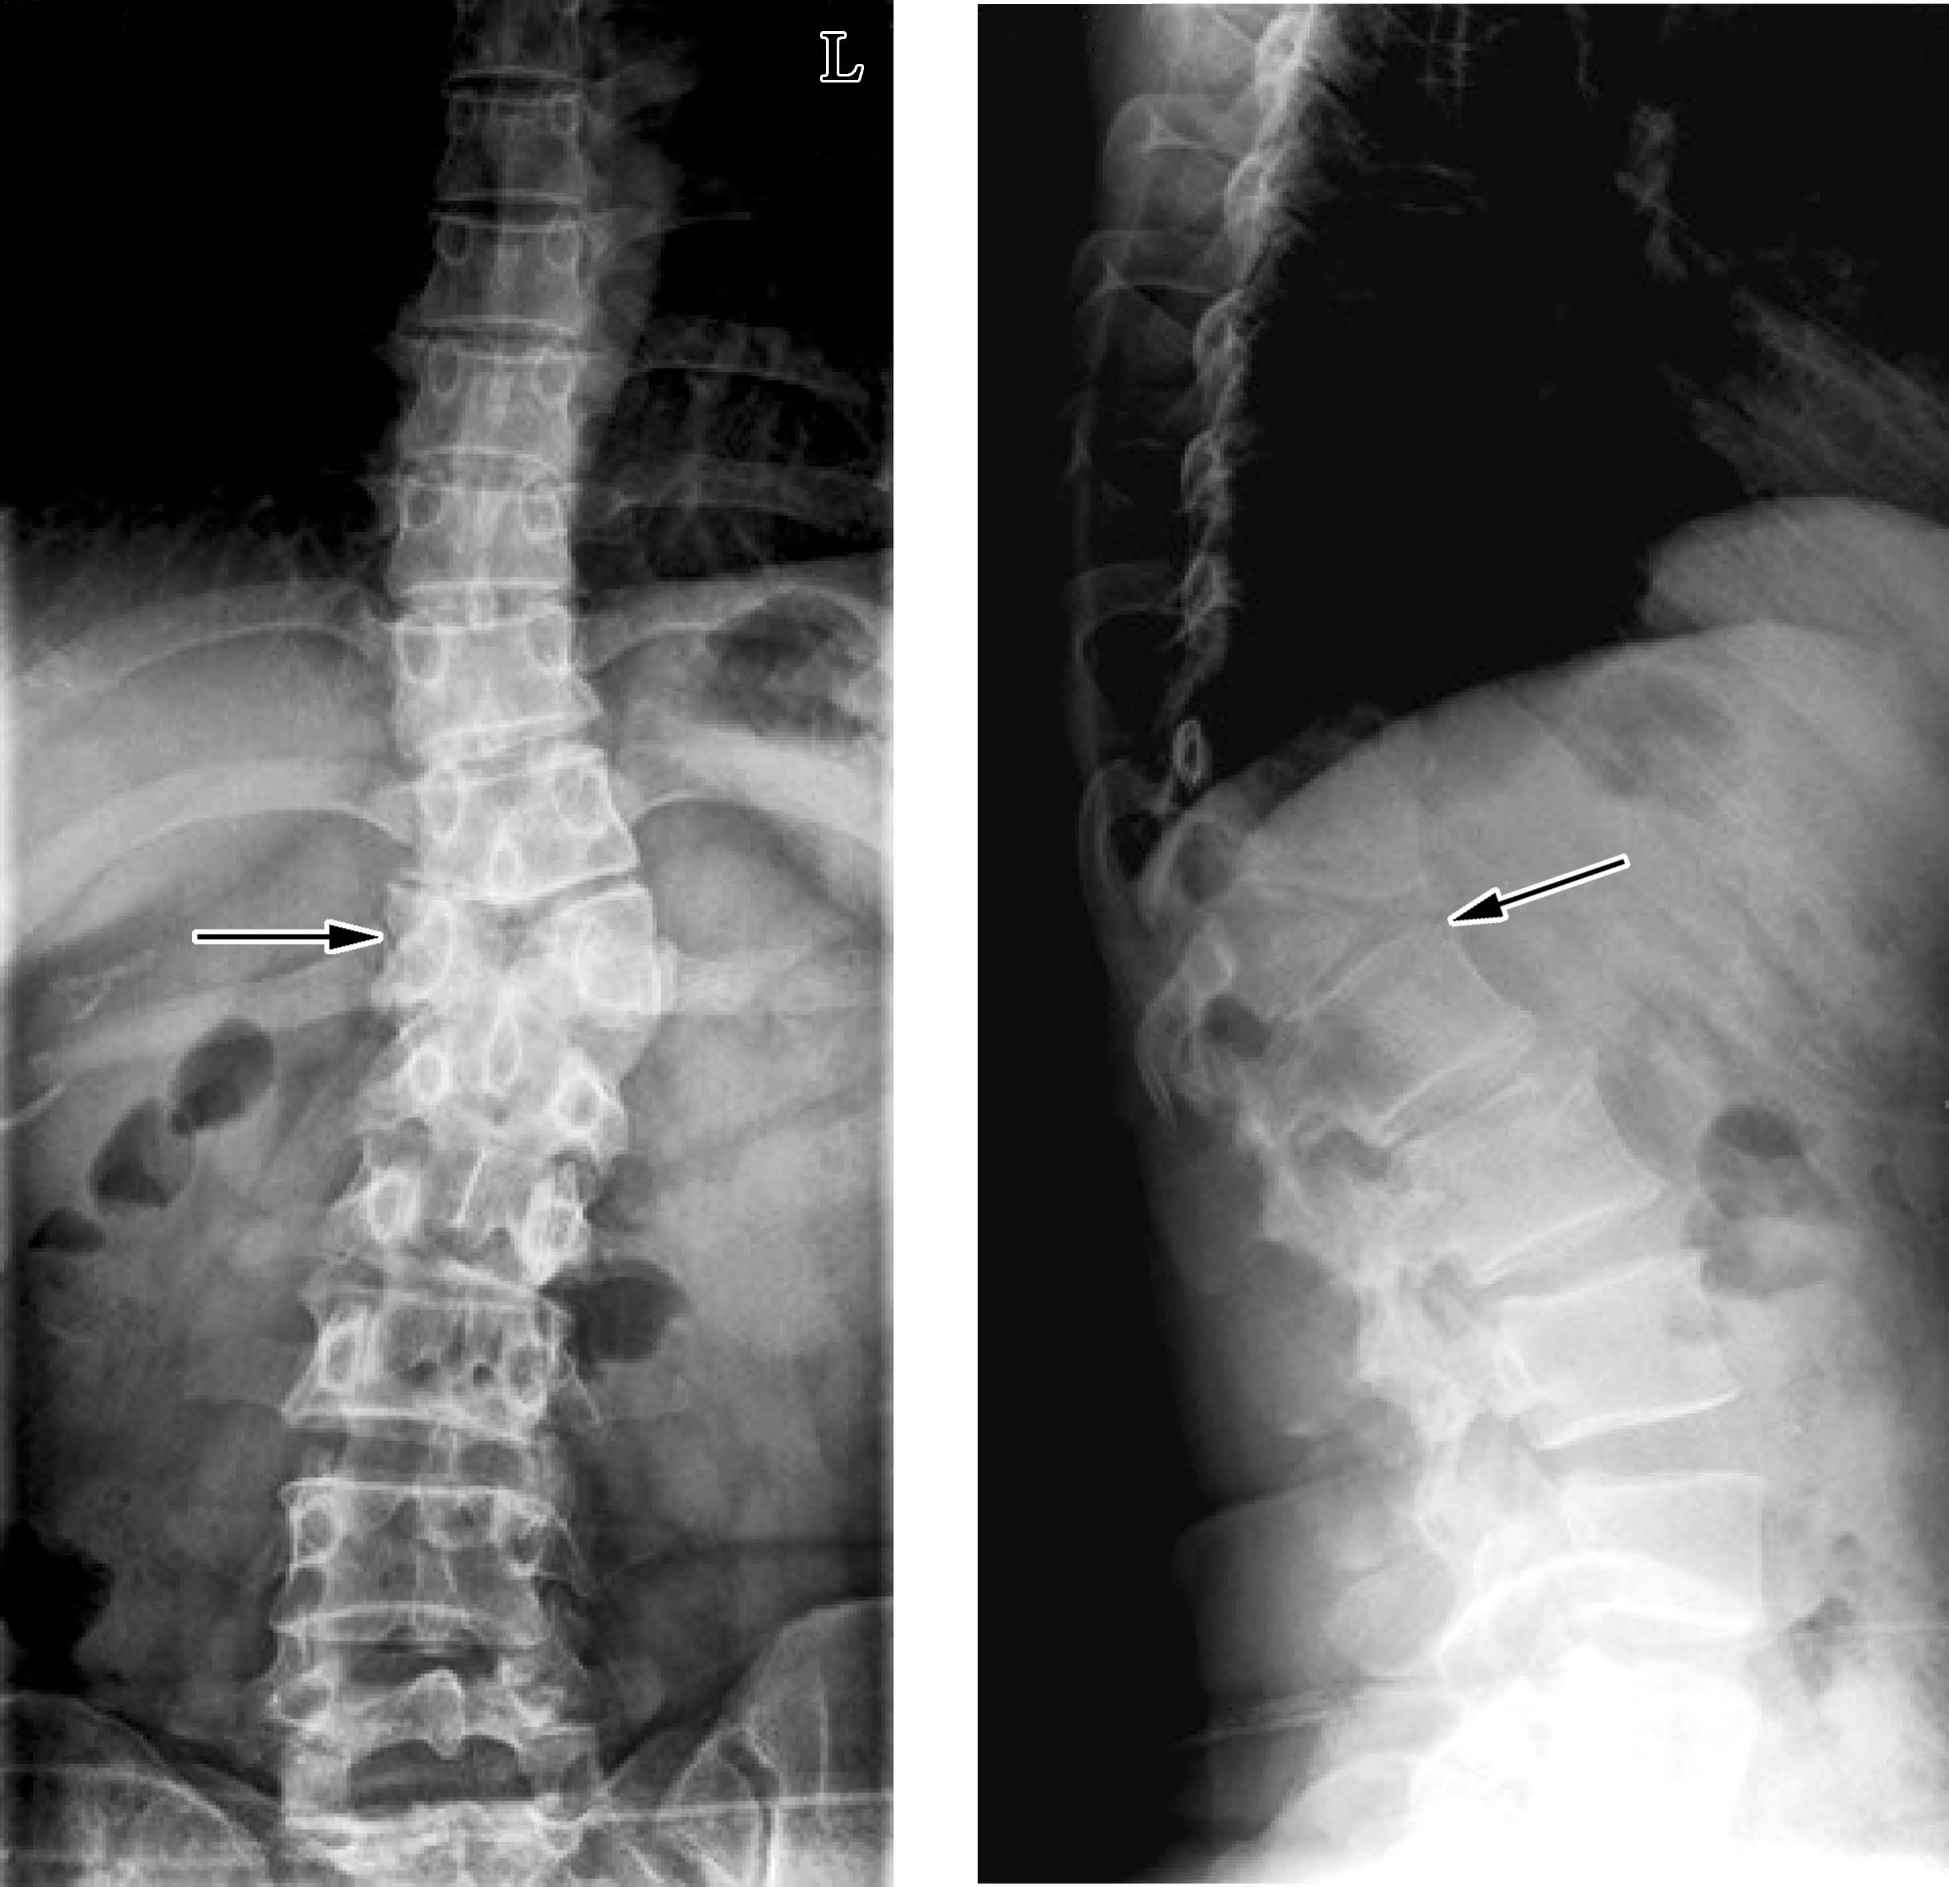
\includegraphics{./images/Image00018.jpg}
 \captionsetup{justification=centering}
 \caption{胸椎正侧位}
 \label{fig2-2-2}
  \end{figure} 

\textbf{【病史摘要】}  女性,38岁。体检发现脊椎有畸形。

\textbf{【X线表现】}
 T12椎体中央部缺如,两半椎体大小形态相似,尖端相对形如蝴蝶,两侧有正常的肋骨连接。

\textbf{【X线诊断】}  T12裂椎畸形。

\textbf{【评  述】}
 胚胎发育时椎体被冠状裂及矢状裂分成前后左右四个骨化中心,若椎体两半部未融合或仅部分融合,则形成裂椎。正位X线片可显示为蝴蝶椎或裂椎。侧位片上椎体影像可显示为中部密度增高的方形或楔形。需要与椎体骨折鉴别,后者表现为骨折断端锐利,临床症状更为明显,同时随时间推移,骨折断端骨痂形成,骨折裂隙模糊。

\subsection{先天性肩胛骨高位症}

\begin{figure}[!htbp]
 \centering
 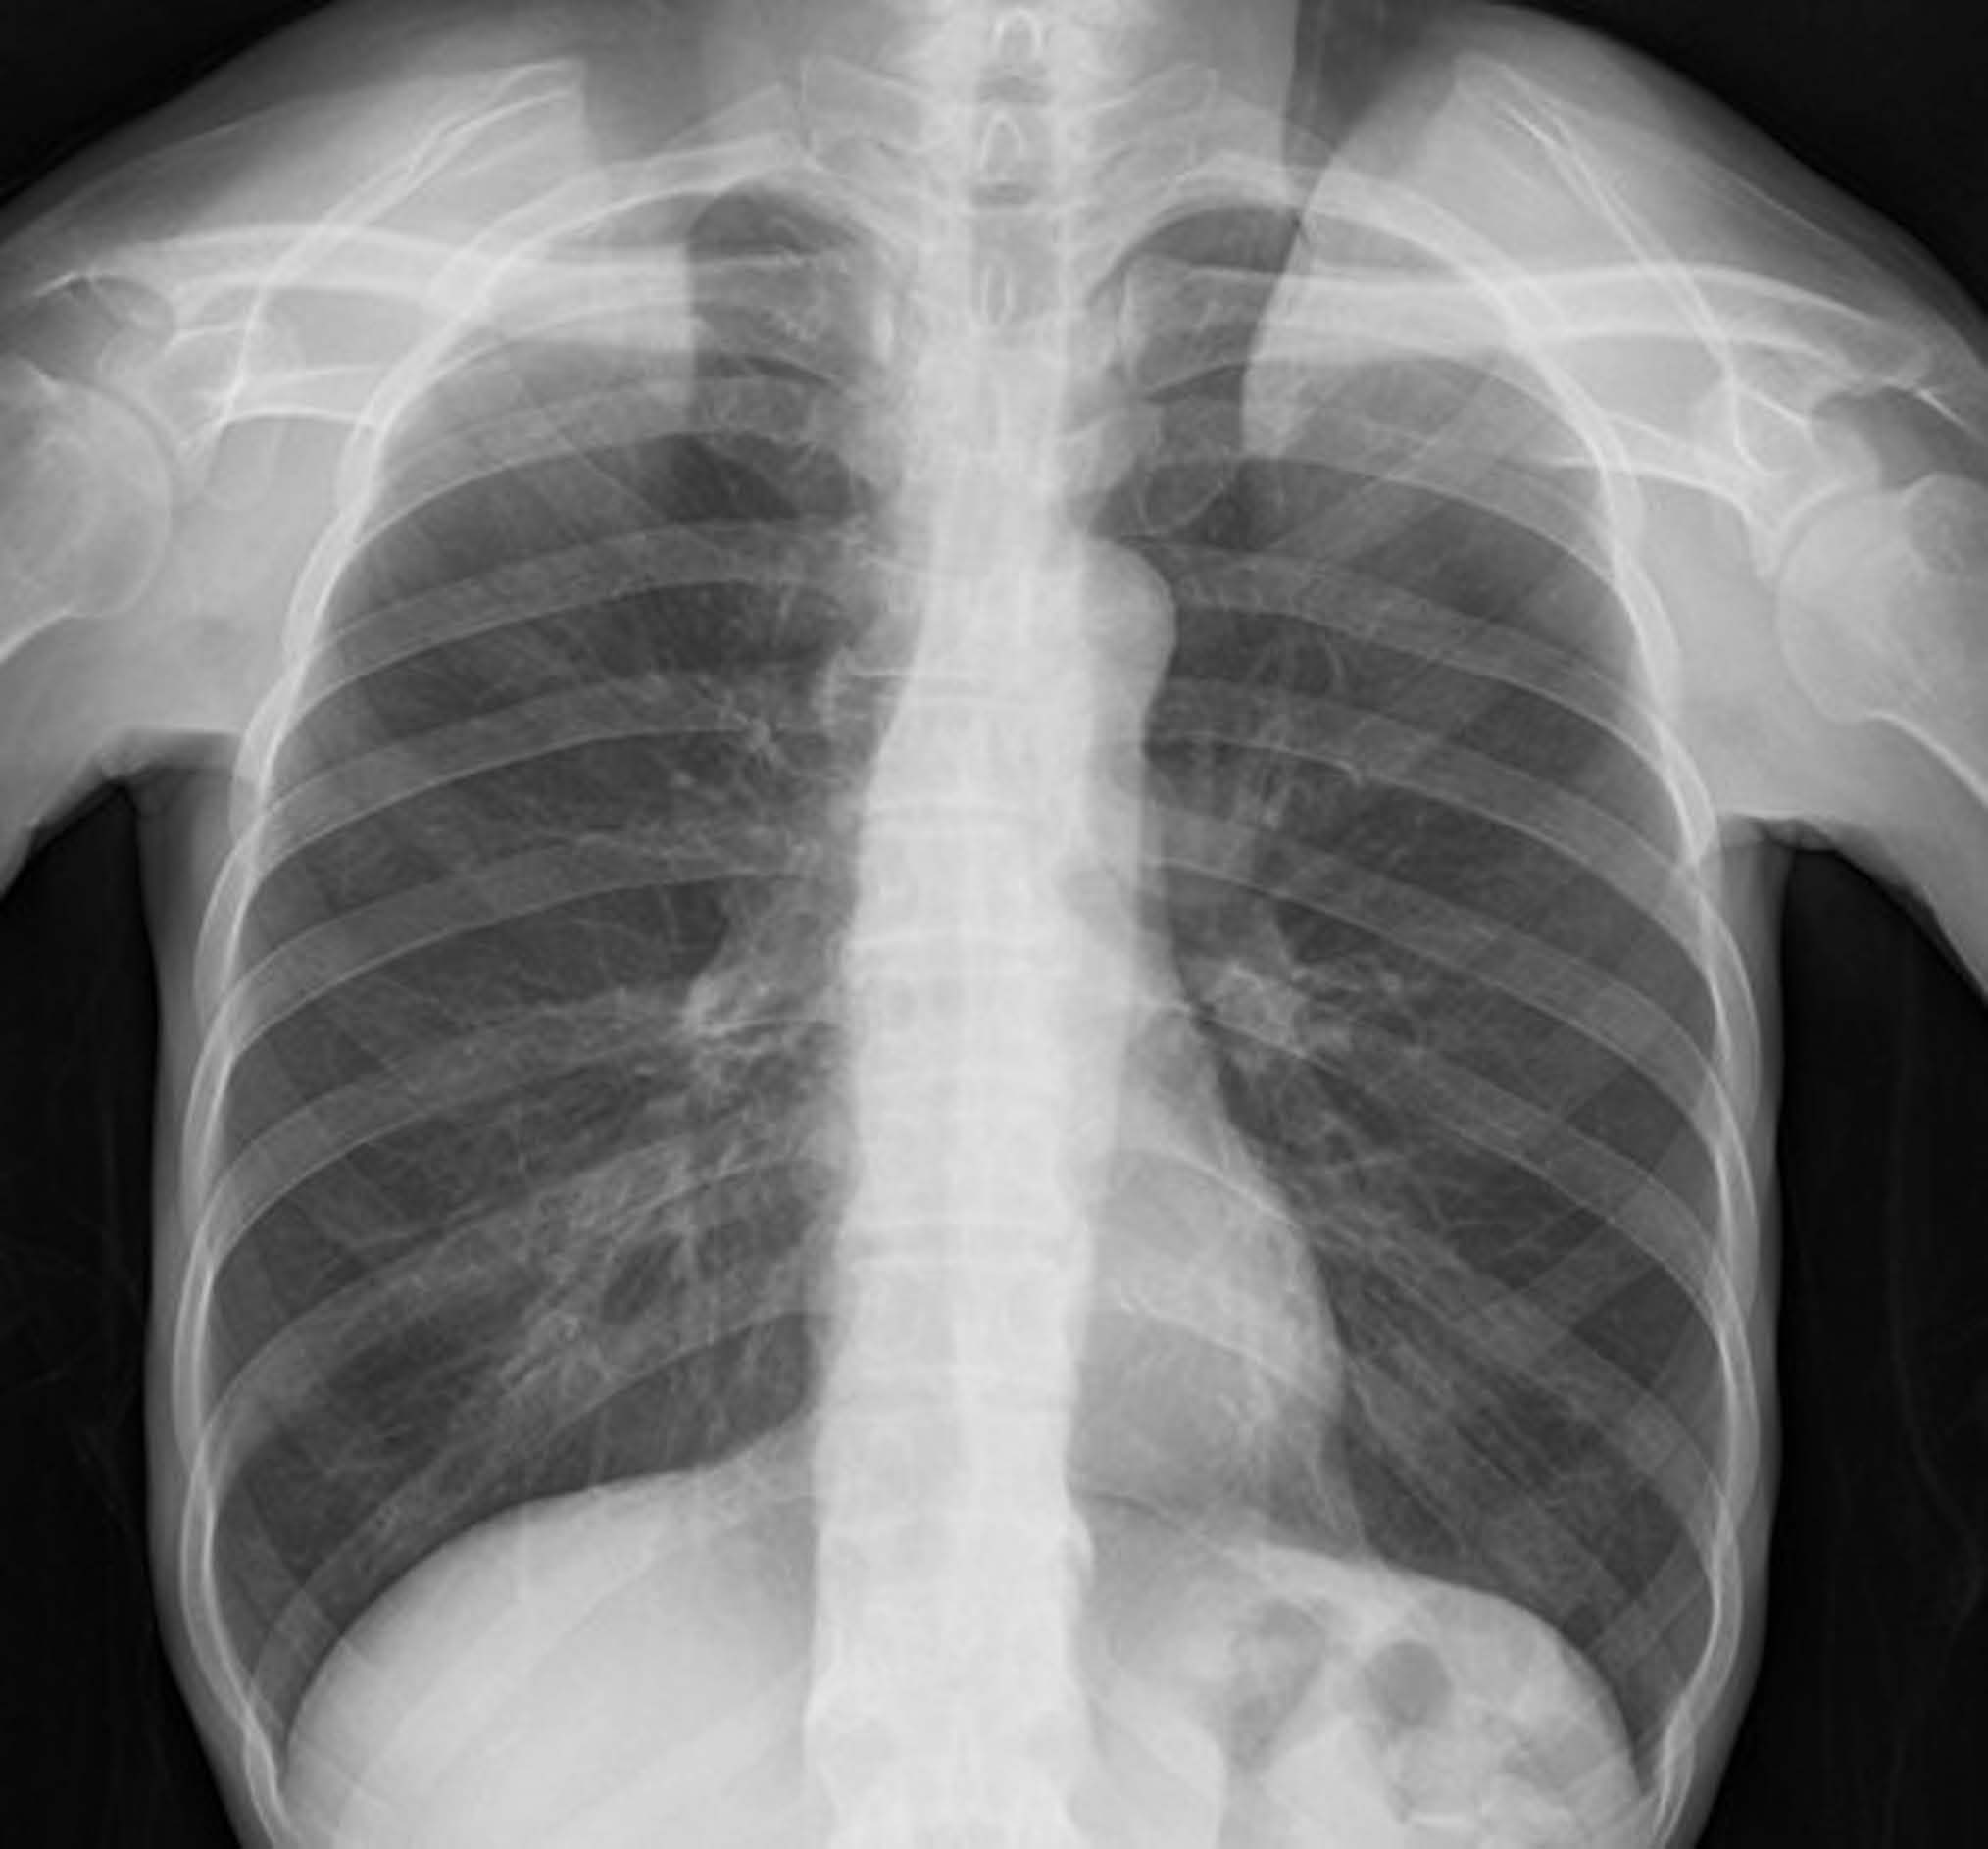
\includegraphics{./images/Image00019.jpg}
 \captionsetup{justification=centering}
 \caption{胸部正位}
 \label{fig2-2-3}
  \end{figure} 

\textbf{【病史摘要】}
 男性,58岁。胸部摄片检查无意中发现肩胛骨位置异常。

\textbf{【X线表现】}
 双侧肩胛骨位置抬高,肩胛骨发育不良,肩胛盂浅而平,肩胛骨下缘向内旋转。

\textbf{【X线诊断】}  双侧先天性肩胛骨高位症。

\textbf{【评  述】}
 本病又称Sprengel畸形、肩胛骨下降不全。是由于胚胎时期,肩胛骨自颈部下降至正常位置过程中出现障碍,导致肩胛骨高位。女性多于男性,两侧均可发病,单侧多见。除肩胛骨高位外,尚可伴有其他骨发育畸形。1/3病例可见到肩胛骨呈桥样连接于颈椎。单侧发病,表现为双侧颈肩部不对称,患侧颈肩部饱满,颈向健侧倾斜;双侧发病,表现为短颈及颈蹼等外观表现。

\subsection{先天性髋关节脱位}

\begin{figure}[!htbp]
 \centering
 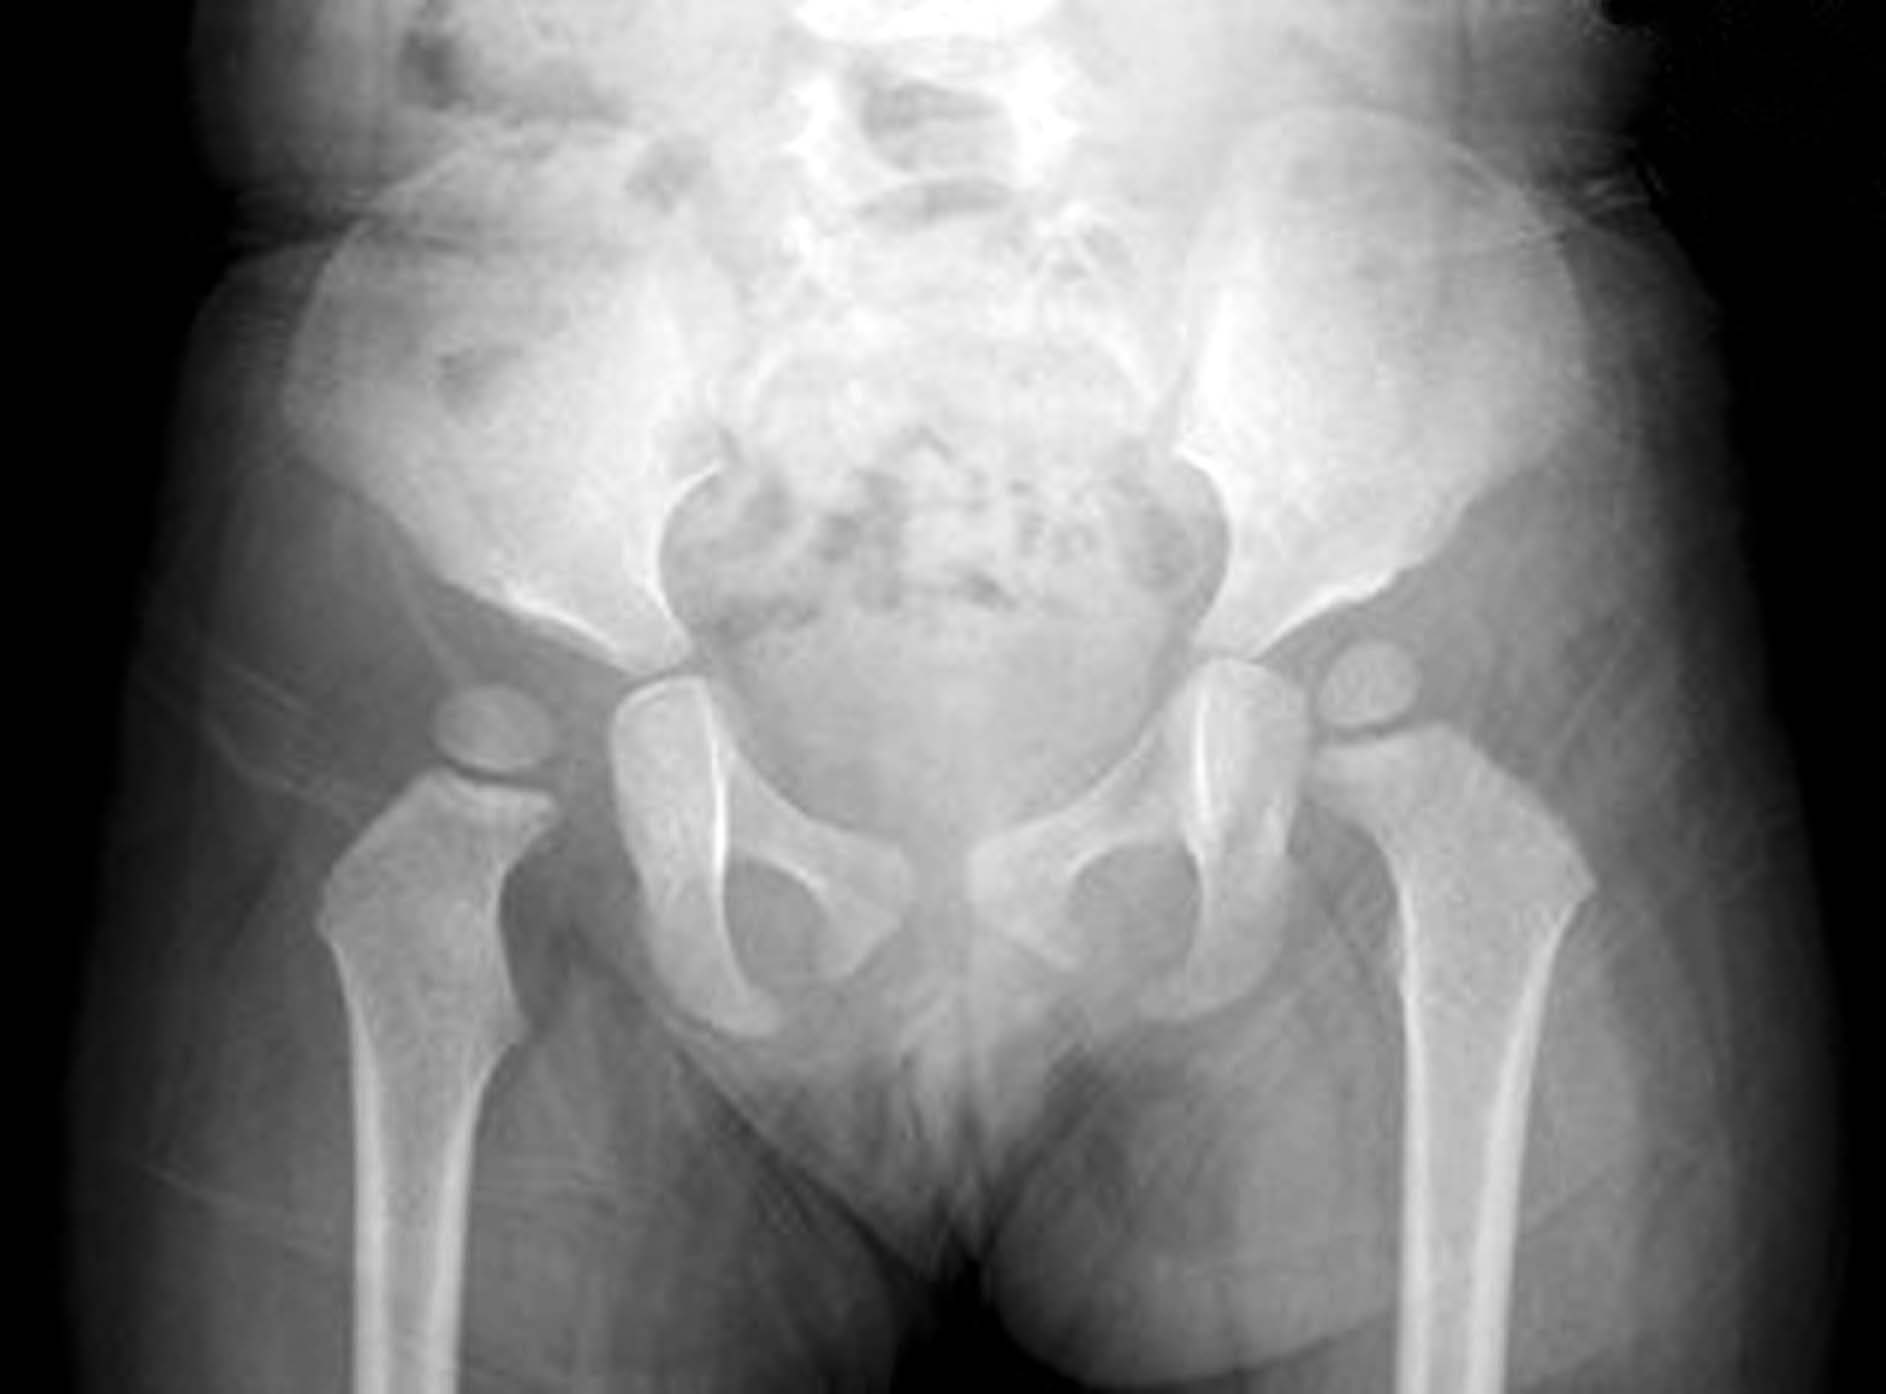
\includegraphics{./images/Image00020.jpg}
 \captionsetup{justification=centering}
 \caption{骨盆正位}
 \label{fig2-2-4}
  \end{figure} 

\textbf{【病史摘要】}  女性,2岁。半年前出现跛行,易摔跤。

\textbf{【X线表现】}
 左侧髋臼浅,髋臼角大于正常值。左侧股骨头发育小,骨骺不光整,并向外上方移位。申通线不连续,股骨头不全位于Perkin方格内下象限。

\textbf{【X线诊断】}  左侧髋关节先天性脱位。

\textbf{【评  述】}
 本病发病原因、机制不明,多为5岁以下女孩,20%有家族史,单侧发病较双侧多见,单侧者出现跛行,双侧者常表现为鸭步,X线片易于诊断。本病需与先天性髋内翻、小儿麻痹后遗症相鉴别。①先天性髋内翻,由股骨近端骨骺局限性的骨化障碍导致,表现为走路跛行或摇晃,患肢外展受限。X线显示股骨颈干角小,股骨头下有三角形碎块影。②小儿麻痹后遗症,由髋关节周围肌肉麻痹而导致脱位,患肢肌肉萎缩及畸形,曾有发热病史。X线显示髋臼小,股骨头发育圆形,股骨颈变细。目前先天性髋关节脱位的X线诊断见下表,适用于6个月以上儿童。

\begin{center}
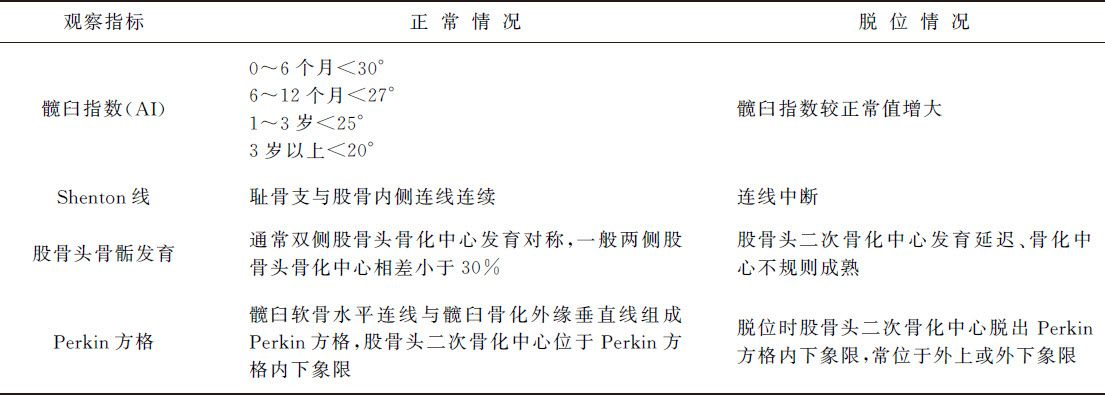
\includegraphics{./images/Image00021.jpg}
\end{center}

\subsection{先天性尺桡骨融合}

\begin{figure}[!htbp]
 \centering
 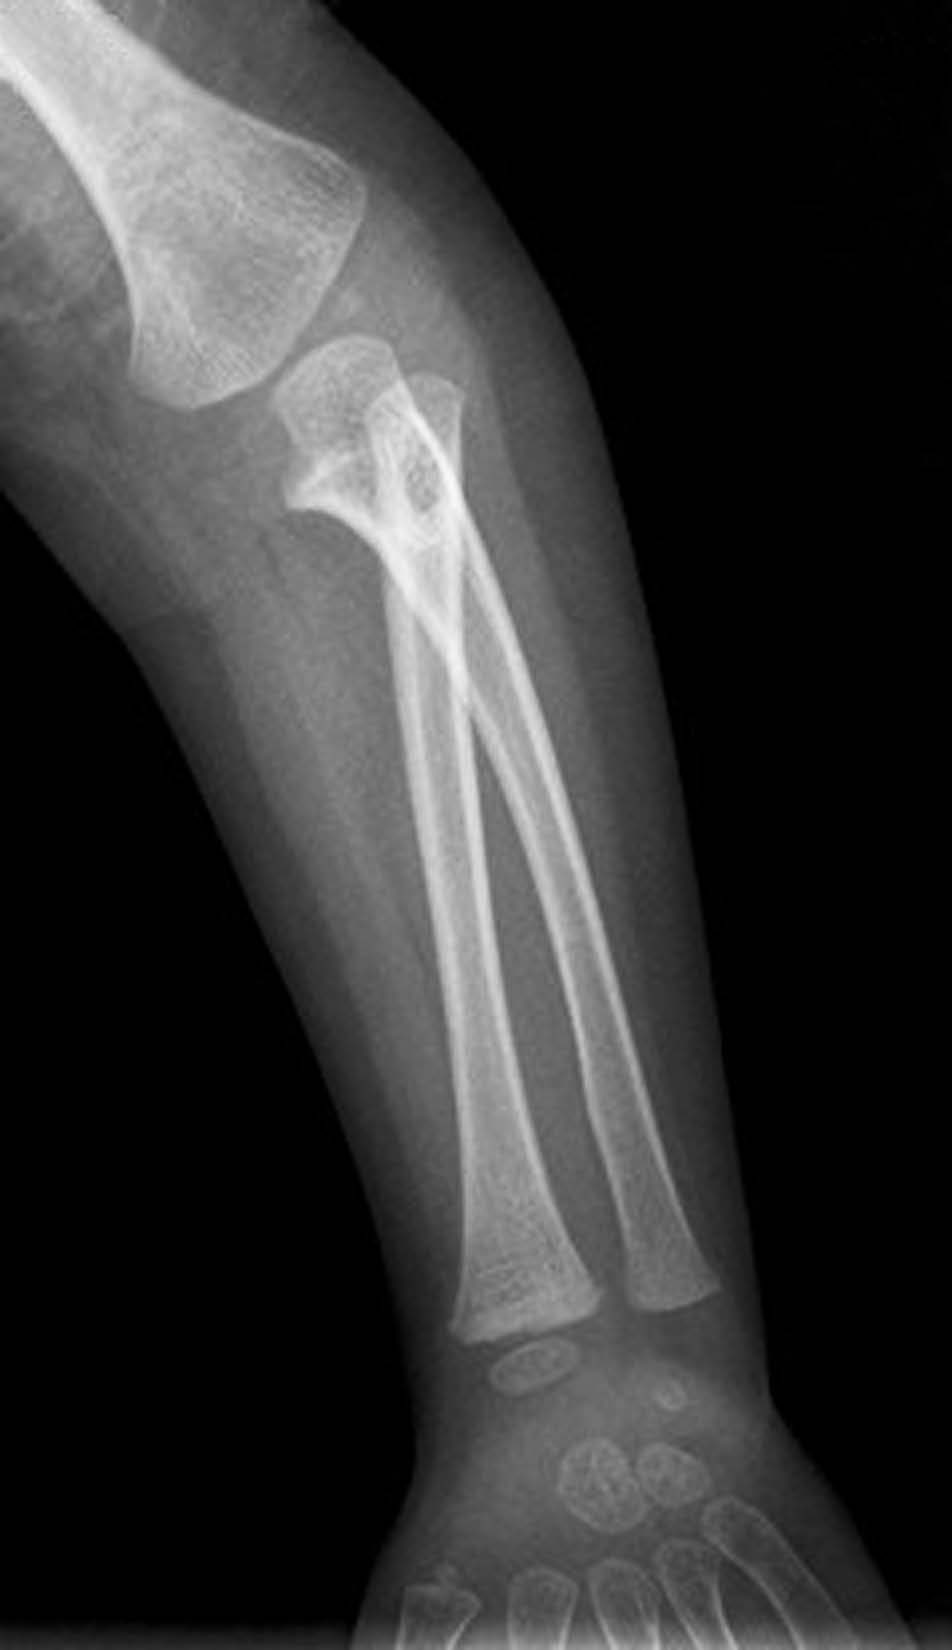
\includegraphics{./images/Image00022.jpg}
 \captionsetup{justification=centering}
 \caption{尺桡骨正位}
 \label{fig2-2-5}
  \end{figure} 

\textbf{【病史摘要】}  男性,2岁。左前臂旋转障碍。

\textbf{【X线表现】}  左尺桡骨近端融合,左侧近侧尺桡关节脱位。

\textbf{【X线诊断】}  左侧先天性尺桡骨融合。

\textbf{【评  述】}
 本病主要表现为尺桡骨近端的骨性联合合并近端尺桡关节脱位,男性多见,单侧或双侧发病。因尺桡骨联合,前臂失去旋转功能。本病需与尺桡骨骨干双骨折内固定术后前臂旋转功能障碍鉴别。首先,后者有手术史,临床上鉴别较简单;其次,当致伤暴力大、损伤范围广、骨折内固定术后肢体外固定的体位不当、制动时间过长及手术操作技术失误等,亦是导致前臂旋转功能障碍的主要原因,故应认真地问清病史。

先天性尺桡骨融合畸形是桡尺骨近端先天融合,前臂固定在一定角度上的旋前位罕见畸形。双侧受累者占60%。男女无差别。该病偶有显性遗传性。发病机制为在胚胎发育中尺桡骨均起自中胚层组织。当胚胎第5周时,尺桡骨软骨杆之间不发生分离而骨化或尺桡骨之间填充中胚层组织时则发生尺桡骨融合。该病无自愈倾向,随年龄增长有加重趋势,必须手术治疗。

X线可以明确融合的部位及程度,为手术提供帮助,若X线显示角度欠佳,可行CT三维扫描观察骨融合细节。

\subsection{马德隆畸形}

\begin{figure}[!htbp]
 \centering
 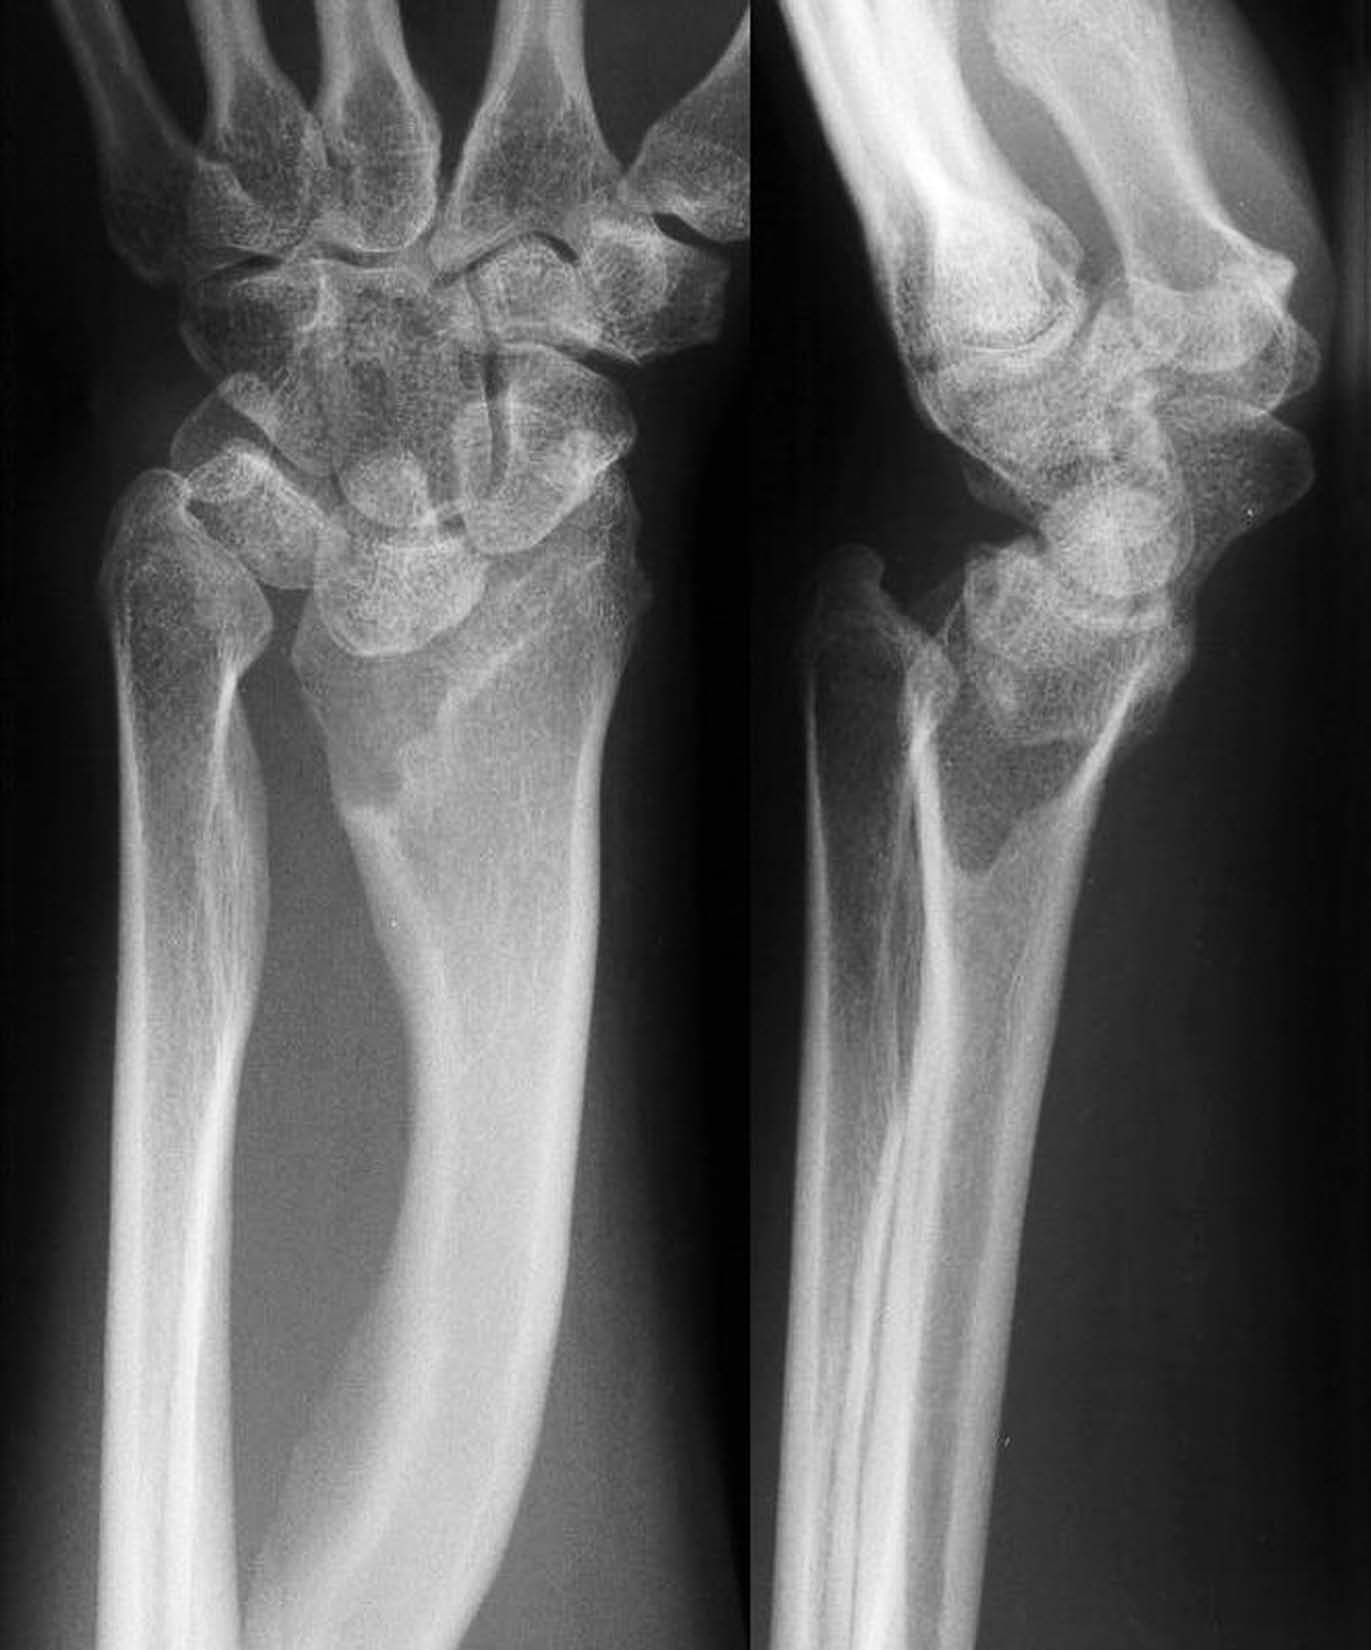
\includegraphics{./images/Image00023.jpg}
 \captionsetup{justification=centering}
 \caption{腕关节正侧位}
 \label{fig2-2-6}
  \end{figure} 

\textbf{【病史摘要】}  女性,34岁。发现右前臂畸形多年。

\textbf{【X线表现】}
 右桡骨呈弓形缩短,并向外侧突出,桡骨关节面向尺侧倾斜。尺骨相对变长,尺骨茎突向背侧突出,远端尺桡关节半脱位,近排腕骨失去正常光滑弧线而呈锥形。

\textbf{【X线诊断】}  右腕马德隆畸形。

\textbf{【评  述】}  马德隆畸形(Madelung
deformity)又称为腕关节发育异常。本病系桡骨远端骨骺内侧发育障碍所致。原因不明,多为先天遗传,以女性发病多见,两侧发病较单侧为多,需与假性马德隆畸形鉴别,假性者常因骨骺外伤而无桡骨发育畸形。典型的X线表现鉴别难度不大,但是本病仍需与腕部或桡骨远端外伤后出现的马德隆畸形、畸形愈合的Colles骨折及Ollier病所造成的假性马德隆畸形相鉴别。因此,详细询问病史对本病诊断比较重要。本病患者大多数身高较矮并有双侧畸形,当伴发其他畸形如短而弯曲的胫骨、短的腓骨、膝外翻就叫作软骨骨生成障碍。而假性马德隆畸形多是由于青少年创伤产生的腕关节类似畸形。

先天性发育畸形与正常变异鉴别非常重要,因为前者需要治疗,后者则无需治疗。当怀疑先天性畸形时,需注意以下三点:①病变是否为孤立性或单发;②病变是否为对称性发病;③病变是否为全身性或多部位。

常见的先天性畸形包括孤立性病变和全身性病变。孤立性病变可根据病变发生的解剖部位来进行更精确的分类,并且可伴发其他类型的先天性或发育性异常。全身性疾病则有许多先天性疾病不同程度地累及骨骼系统,大部分非常罕见,诊断需要凭借X线检查。

\subsection{右手多指}

\begin{figure}[!htbp]
 \centering
 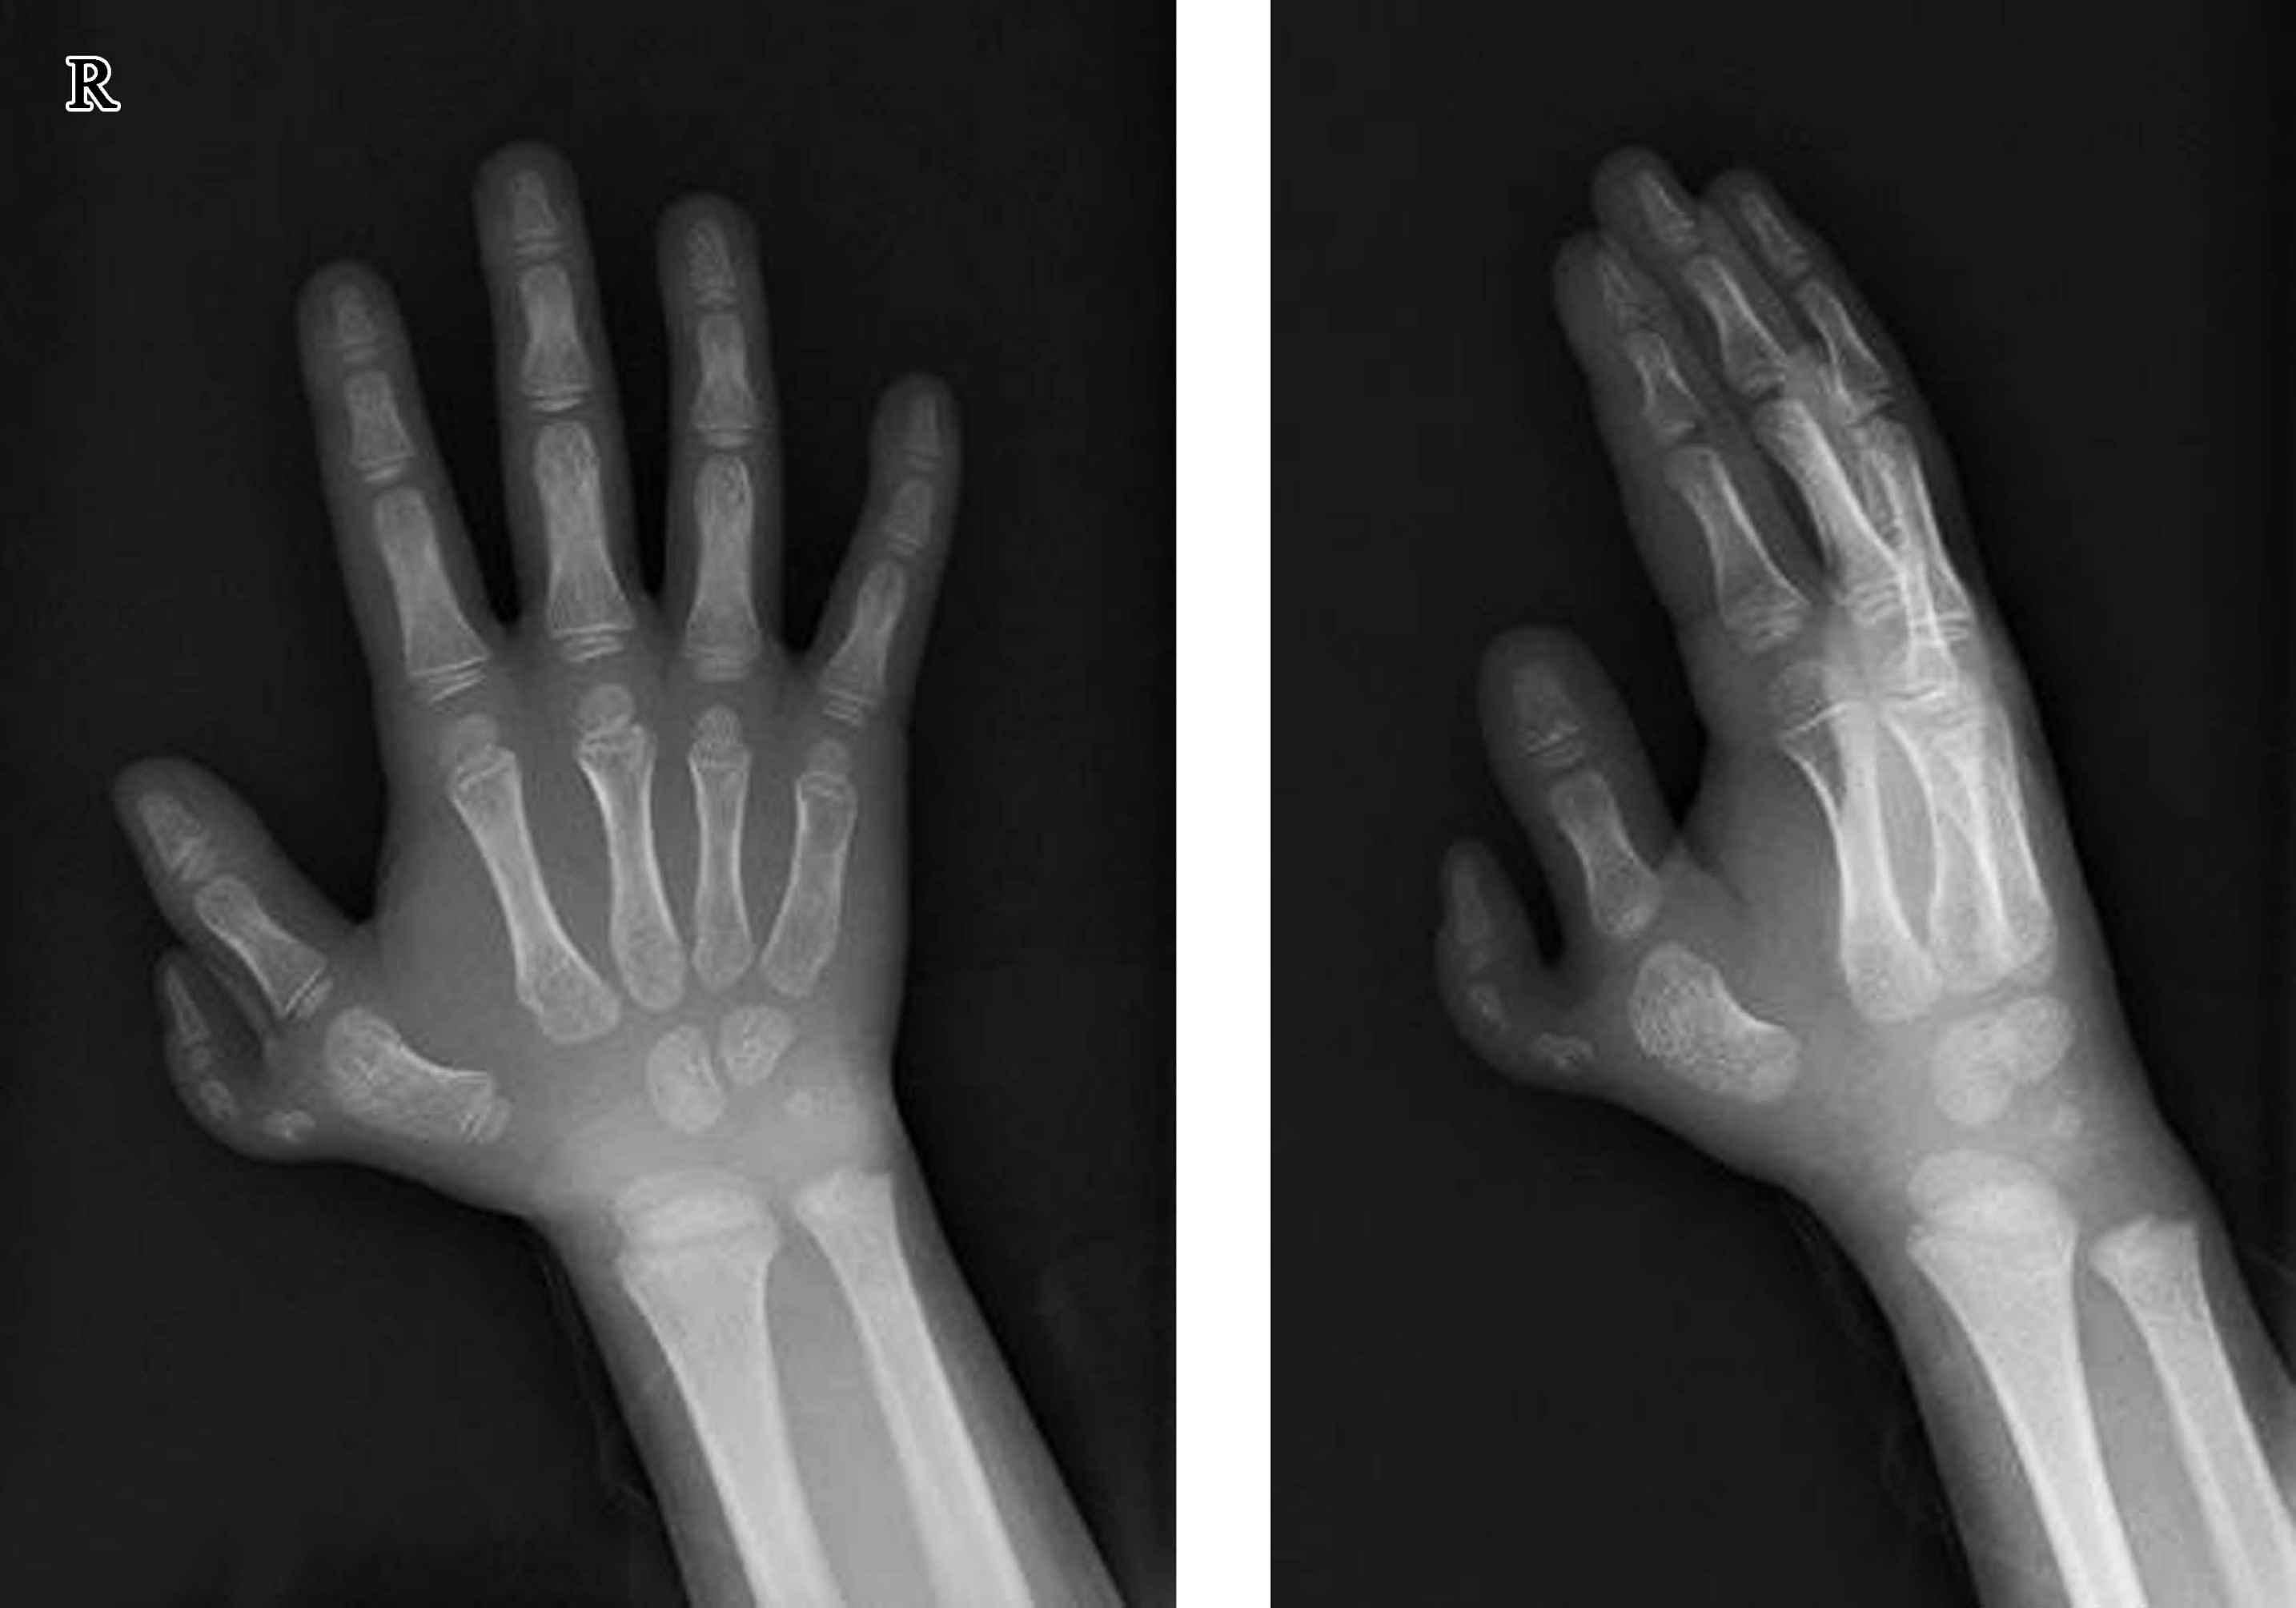
\includegraphics{./images/Image00024.jpg}
 \captionsetup{justification=centering}
 \caption{右手正斜位}
 \label{fig2-2-7}
  \end{figure} 

\textbf{【病史摘要】}  男性,4岁。发现右手多指多年。

\textbf{【X线表现】}
 右手拇指外侧多生指,含有指骨,并与第一掌骨头构成关节。

\textbf{【X线诊断】}  右手多指畸形。

\textbf{【评  述】}
 多指,又称额外手指,多为六个手指,多者可达八个,发生在拇指或小指旁。一般分为三型:①软组织型,仅为一赘生的软组织,内无骨和软骨。②多生指型,最常见,与正常指骨一样,含有指骨并与掌骨构成关节,掌骨关节增大或呈分叉状。③多指骨型,即在固有的掌骨上发生两指骨或指骨有分叉,少见。本例为多生指型。本病诊断不难,准确的分型对临床指导意义更大。

先天性多指(趾)多为单侧性,双侧受累仅占10%左右。复拇畸形确切病因不明,大多为散发,提示该病与环境因素有关,与遗传因素关系不大。并指(趾)常伴发心血管、神经系统或泌尿系统的畸形,例如先天性心脏病、先天性脑发育不良等,对有疑似的患儿应进行全面系统的体格检查。

\subsection{并趾}

\begin{figure}[!htbp]
 \centering
 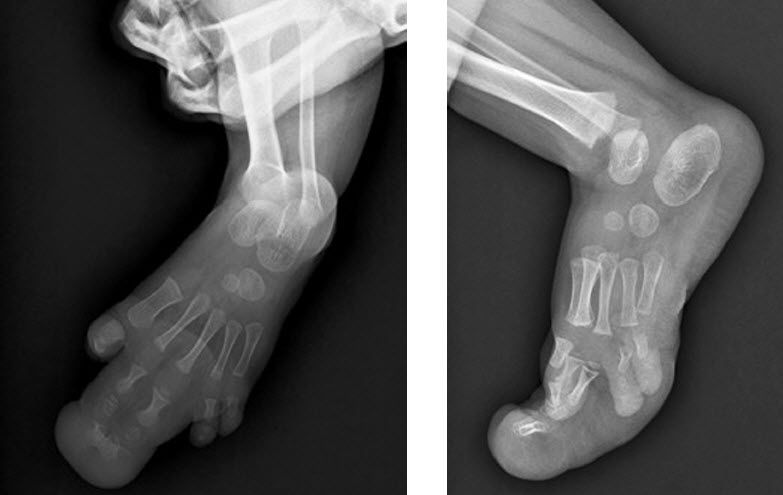
\includegraphics{./images/Image00025.jpg}
 \captionsetup{justification=centering}
 \caption{足正斜位}
 \label{fig2-2-8}
  \end{figure} 

\textbf{【病史摘要】}  男性,2岁。发现左足畸形2年。

\textbf{【X线表现】}  左足第2、3趾骨骨性融合,左足第1、4、5趾短小。

\textbf{【X线诊断】}  左足第2、3趾并趾,并左足第1、4、5趾短趾畸形。

\textbf{【评  述】}
 并指(趾),单、双侧均可发生,常发生在第3、4指(趾)间,亦可多指合并,拇指(趾)极少累及。连接并趾间的组织可仅为软组织,也可为骨连接。常并发多趾、短趾畸形。本病诊断不难,临床分为软组织并趾和骨性并趾。前者骨骼发育正常,关节完整,可以屈伸。最轻者两趾间仅有一层薄薄的蹼,似鸭掌。重者两趾靠近,中间有软组织连接,外观似一巨趾,但X线示骨骼完全分开。后者两趾骨骼合并,轻者仅有部分趾骨粘连,一般近1、2节分开,末节趾骨连接,有的趾甲合拢。重者两趾骨完全融合,甚至关节亦不存在。

并指畸形既可以是单独出现,也可以是其他畸形或综合征的症状之一,如常见的在先天性手畸形中伴有并指畸形;如多指并指、短指并指、分裂手并指、指端交叉并指、肢体环状狭窄合并并指、手发育不良并指、Apert综合征、Poland综合征等。

\subsection{股骨滑车发育不良}

\begin{figure}[!htbp]
 \centering
 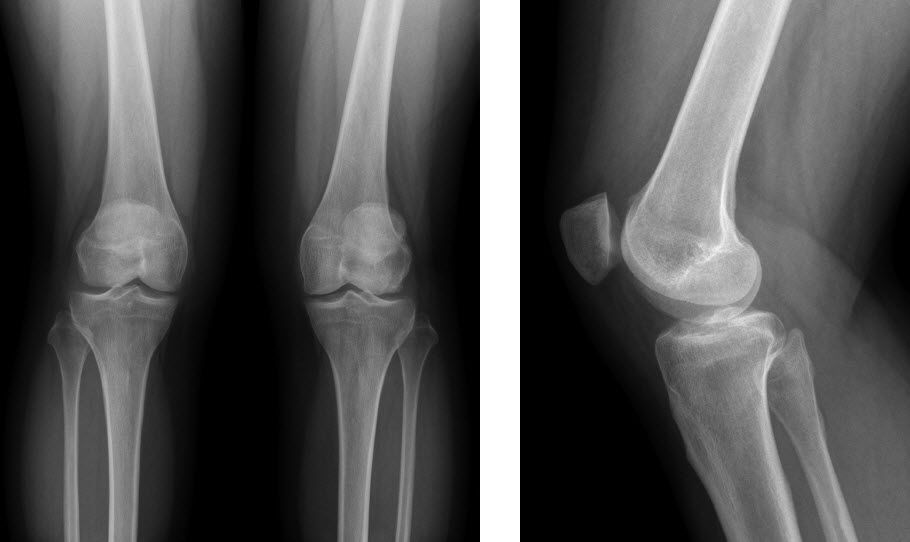
\includegraphics{./images/Image00026.jpg}
 \captionsetup{justification=centering}
 \caption{膝正侧位}
 \label{fig2-2-9}
  \end{figure} 

\textbf{【病史摘要】}  女,28岁。双侧髌骨不稳定,膝部反复疼痛。

\textbf{【X线表现】}
 X线正位片示双侧髌骨呈明显高位,髌骨位于股骨滑车上缘。侧位片示右侧髌骨呈明显高位,股骨滑车沟向前突起,滑车沟线与股骨外侧髁线形成交叉。

\textbf{【X线诊断】}  股骨滑车发育不良伴双侧髌骨高位征。

\textbf{【评  述】}  股骨滑车发育不良(Femoral Trochlear
dysplasia,FTD)是指滑车沟的几何外形和深度存在解剖学异常,尤其是滑车上部。当出现FTD时髌骨与股骨滑车近端不能稳定衔接,可在伸直位或屈曲早期发生半脱位,出现髌骨不稳定、膝部疼痛等症状。髌股关节运动轨迹也可出现异常,从而引发髌股关节骨关节炎。膝关节侧位X线片是对FTD诊断的最佳投照位置。股骨滑车的形态分为以下几种:①正常股骨滑车:A型:滑车沟线与股骨髁前缘线无交叉;B型:滑车沟线仅与内髁前缘线相交叉。②FTD,滑车沟线与内、外髁前缘线皆相交:Ⅰ型:交叉征对称,位于滑车近端;Ⅱ型:交叉征不对称,先与内髁相交,然后与外髁相交;Ⅲ型:交叉征位于内、外髁下端。③中间态股骨滑车:Ⅰ型:滑车沟在股骨髁前缘附近延续为股骨干,但无交叉征;Ⅱ型:滑车沟与内髁前缘交叉,但不与外髁相交。FTD主要X线表现为:交叉征和滑车沟突起。交叉征指滑车沟底与股骨外侧髁的轮廓线相交叉。滑车沟底的突起指沿股骨干向其远端作延长线(代表滑车沟底平面),平行于该线作股骨髁的切线,两条直线的线间距即代表突起的大小,此值超过3mm即为滑车沟突起,可诊断为股骨滑车发育不良。

图2-2-10为前片的X线侧位片放大图和CT横断位。前者示弧形的滑车沟底线(点状虚线)与股骨外侧髁的轮廓线(黑色实心线)交叉,此“交叉征”是股骨滑车发育不良的特征性表现;沿股骨干延长线作一平行线(1线),沿滑车底腹侧点作平行于1线的直线(2线),两线之间的距离即为滑车沟突起距离,该距离远大于3mm,即为滑车沟突起。两个指标即可诊断股骨滑车发育不良。CT横断位示股骨滑车沟明显变浅,股骨滑车外侧髁发育不良,髌骨向外侧脱位,关节腔内见少量积液。

\begin{figure}[!htbp]
 \centering
 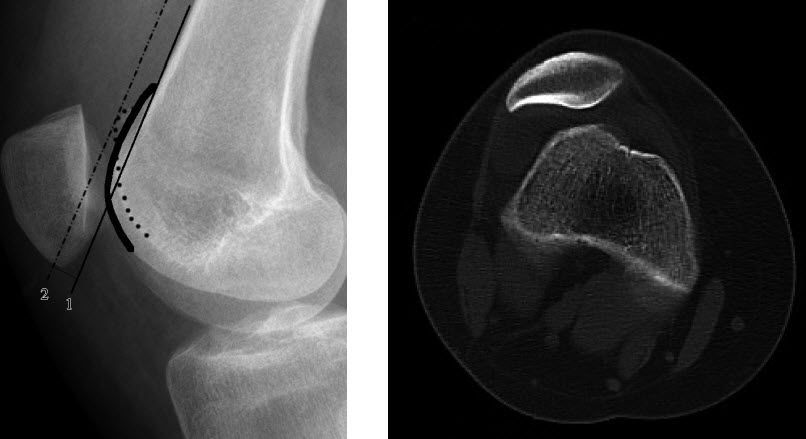
\includegraphics{./images/Image00027.jpg}
 \captionsetup{justification=centering}
 \caption{膝X线侧位及CT横断位}
 \label{fig2-2-10}
  \end{figure} 

CT横断位上股骨滑车发育不良分为四种类型:①相对较浅的滑车沟;②扁平或突出的滑车沟;③滑车关节面不对称,外侧面突出,内侧面发育不全;④滑车关节面不对称,垂直的关节面与峭壁征。本例即为相对较浅的关节面。诊断该类疾病,目前主要依靠X线片,尤其是侧位片和CT,两者对股骨滑车发育不良的骨性标志诊断确切,但是MRI对该疾病的诊断有更重要的价值,例如MRI可明确关节软骨的损伤和发育情况,对评估患者的病情更有意义。

\section{骨与关节创伤}

\subsection{肩关节脱位}

\begin{figure}[!htbp]
 \centering
 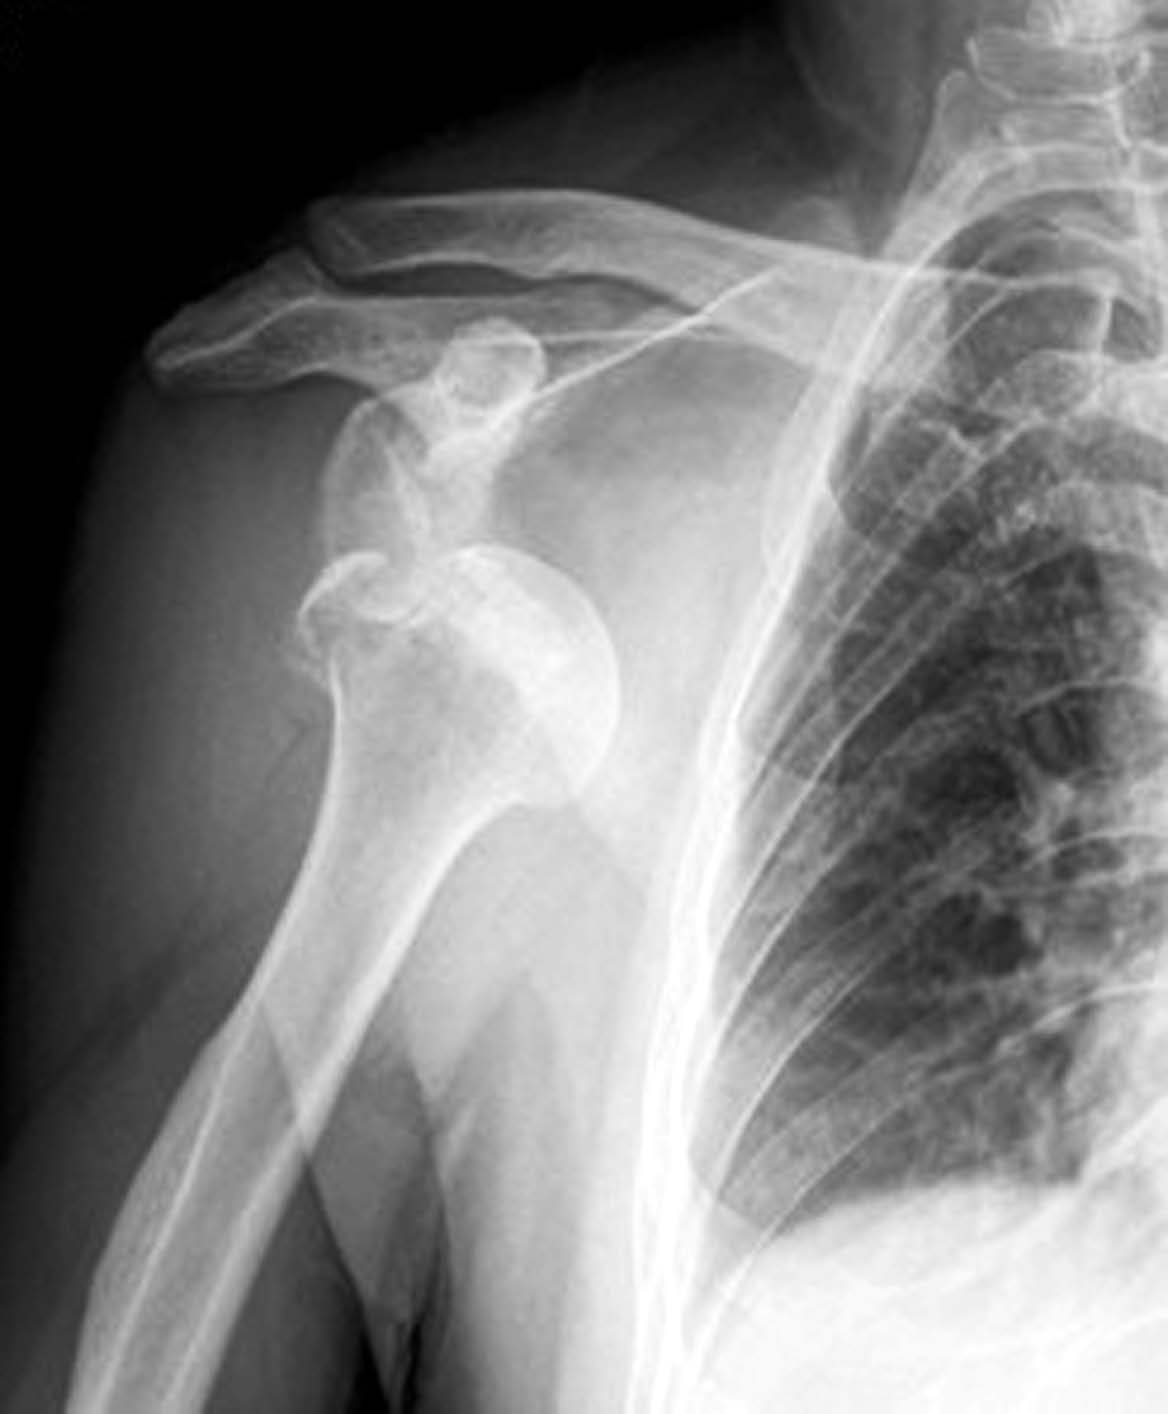
\includegraphics{./images/Image00028.jpg}
 \captionsetup{justification=centering}
 \caption{肩关节正位}
 \label{fig2-3-1}
  \end{figure} 

\textbf{【病史摘要】}
 男性,60岁。跌倒时手外展着地,肩关节肿痛、活动障碍。肩部呈方形。

\textbf{【X线表现】}
 右肱骨头向前下方移位至肩胛盂下方,肱骨大结节处见撕脱小骨片。

\textbf{【X线诊断】}  右肩关节前脱位。

\textbf{【评  述】}
 肩关节解剖特点为关节盂浅,肱骨头大。肩关节的稳定全靠肌肉及韧带维系,容易脱位,在关节脱位中占第二位。肩关节脱位可分为前脱位和后脱位两种,因其前下方缺乏软组织保护,故前脱位最常见(约占肩关节脱位的95%),多为跌倒时手掌着地,肱骨高度外旋及中度外展位,掌面传达到肱骨头的暴力冲破关节囊的薄弱前壁,向前滑出。正位片可见肱骨头与肩盂和肩胛颈重叠,位于喙突下0.5~1.0cm处,肱骨头呈外旋位,肱骨干轻度外展。肩关节后脱位非常少见,在脱位过程中还可造成关节盂唇软骨或后缘骨折。此型易漏诊或误诊。注意体检和侧位观察。准确区分半脱位、前脱位及后脱位是诊断的关键。半脱位关节间隙上宽下窄。肱骨头下移,尚有一半的肱骨头对向肩盂。后脱位的正位片肱骨头与肩盂的对位关系尚好,关节间隙存在,极易漏诊;在侧位片或腋位片才能显示肱骨头向后脱出,位于肩盂后方。

肩关节脱位与年龄有重要关系,35岁以下患者首次脱位易导致前关节盂或关节囊前部撕裂,35岁以上患者则易导致关节肩袖肌撕裂或肱骨大结节撕脱。因此,当出现肩关节脱位时根据患者年龄需要关注:①有无肱骨大结节撕脱性骨折,关节盂及肩袖等有无损伤;②X线检查不能明确以上病变时,应进一步行MRI检查明确诊断。

\subsection{肩关节钙化性肌腱炎}

\begin{figure}[!htbp]
 \centering
 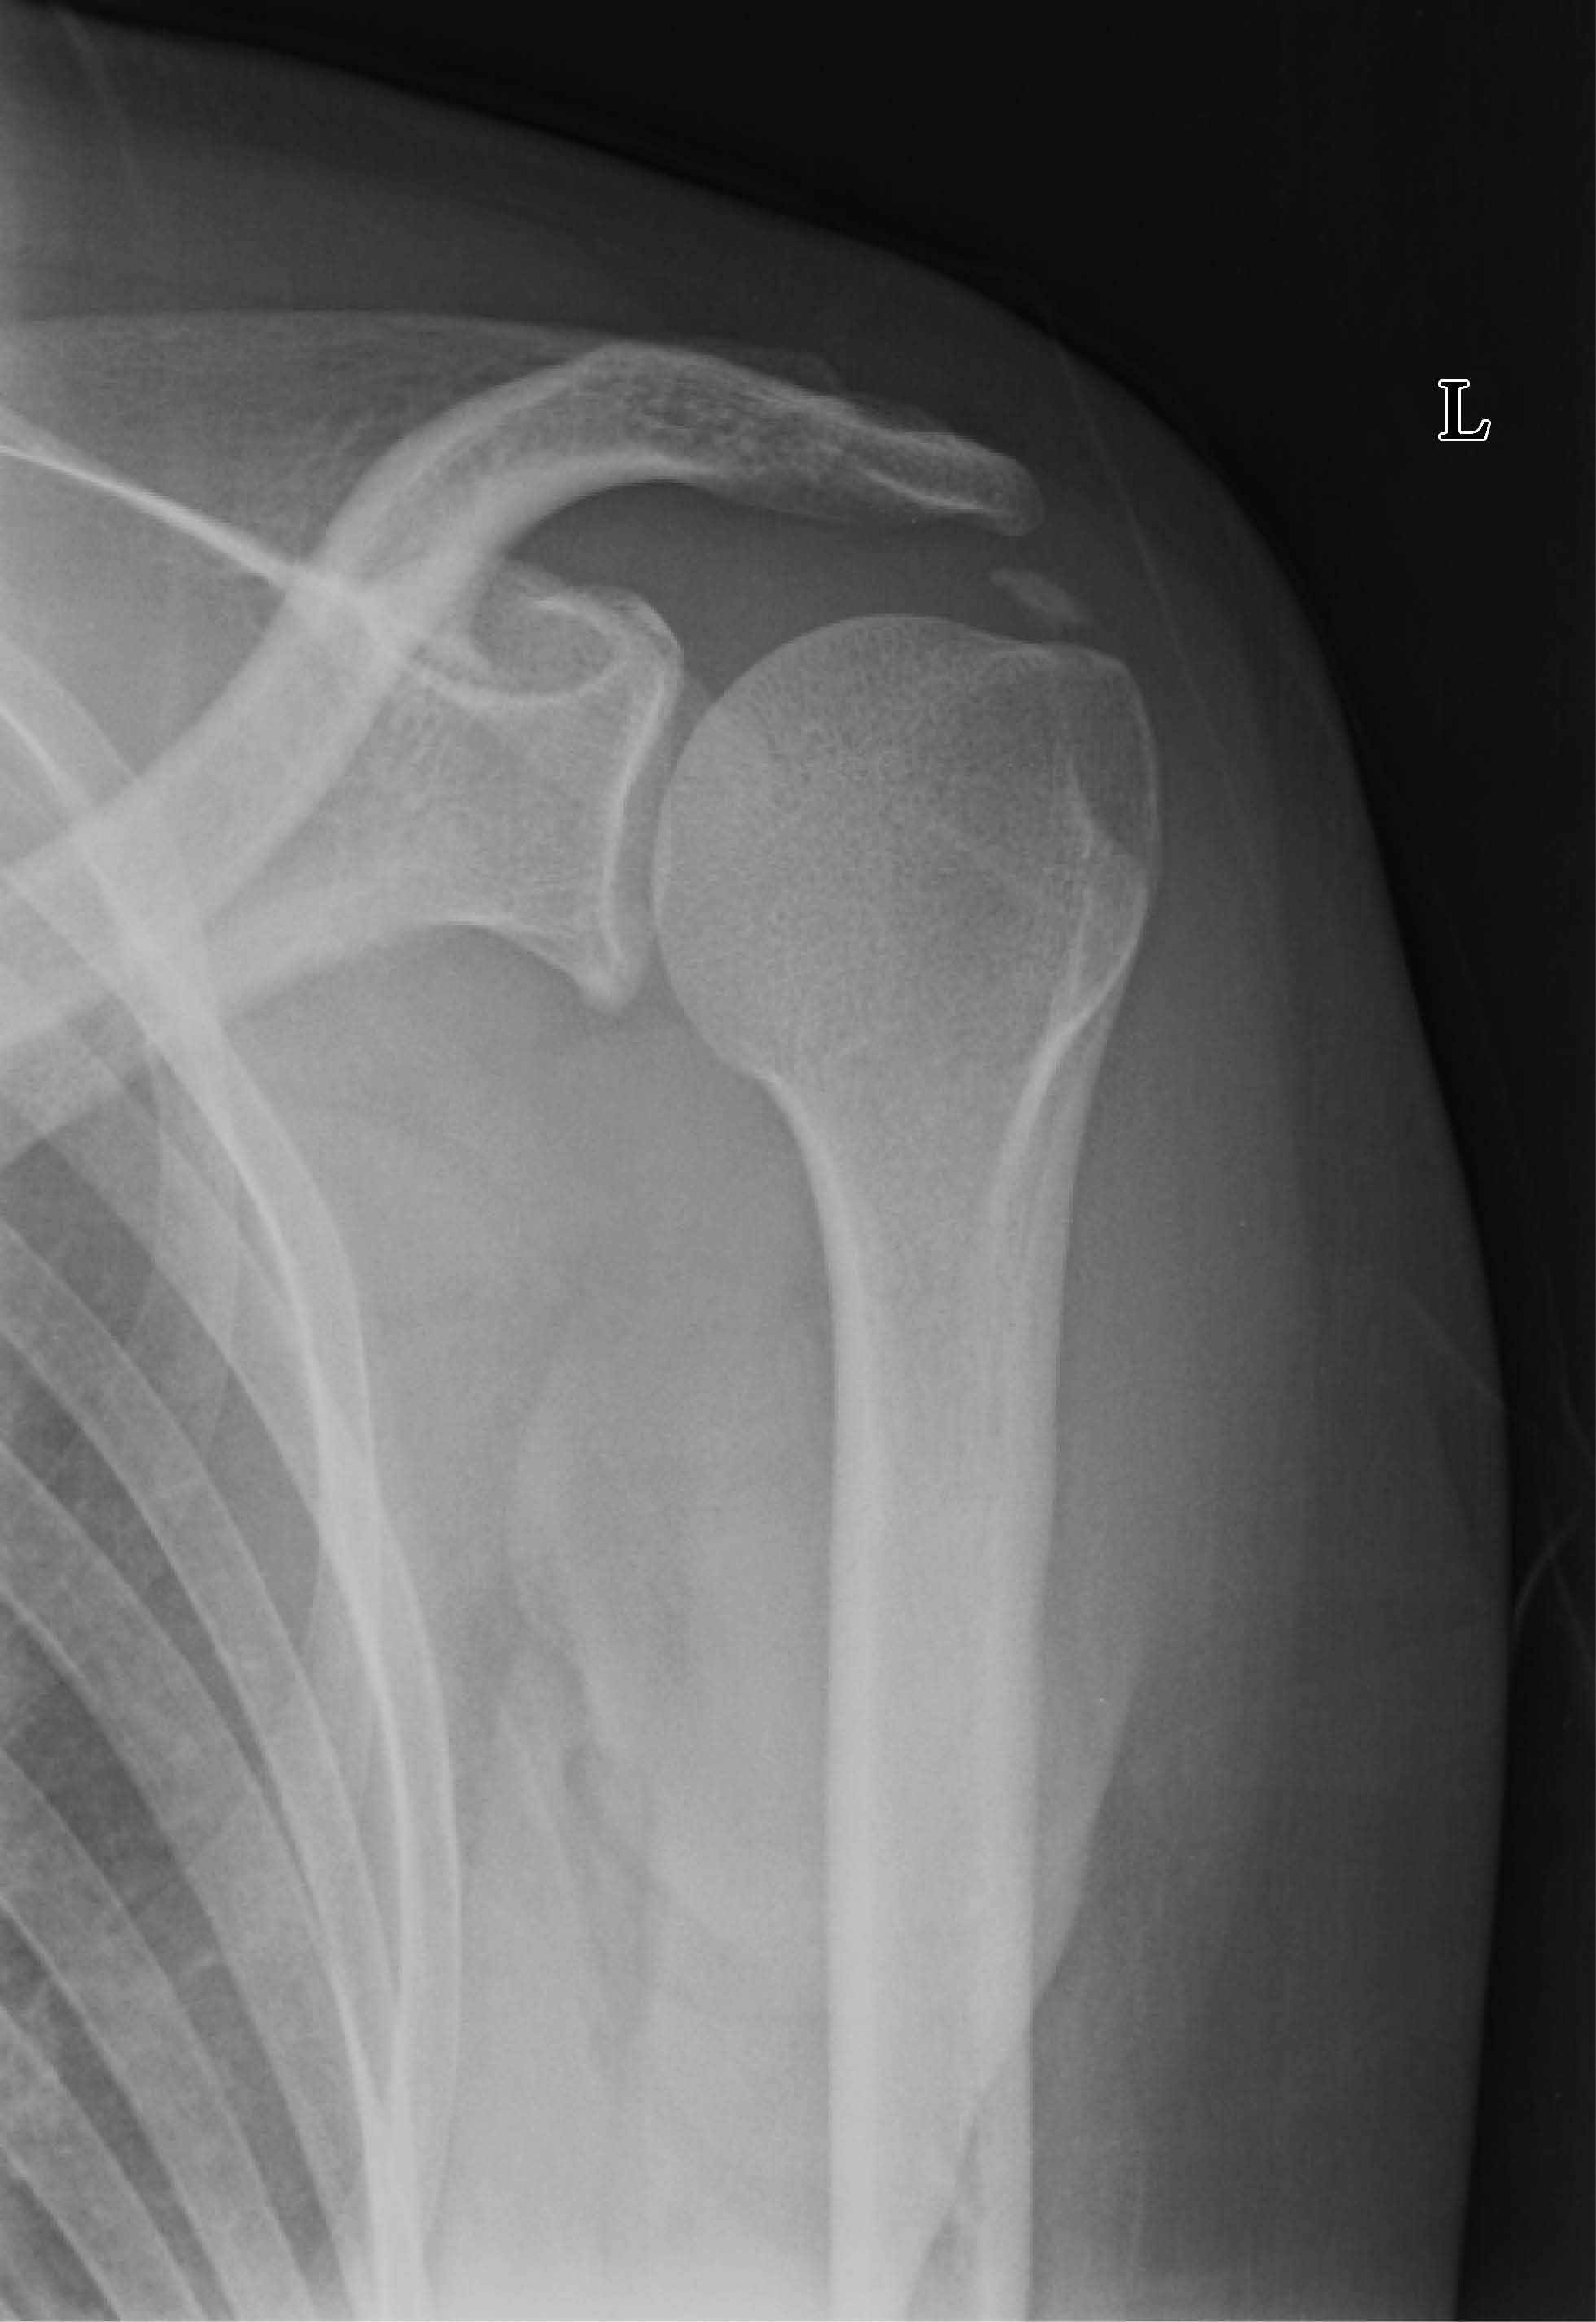
\includegraphics{./images/Image00029.jpg}
 \captionsetup{justification=centering}
 \caption{左肩关节正位}
 \label{fig2-3-2}
  \end{figure} 

\textbf{【病史摘要】}
 女,40岁。左肩关节后方反复疼痛,肱骨大结节处压痛明显。

\textbf{【X线表现】}
 正位片示左肩关节肩袖处可见小片状高密度影,钙化边缘模糊不光整,周边软组织未见明显肿胀。

\textbf{【X线诊断】}  左肩关节钙化性肌腱炎。

\textbf{【评  述】}
 肩关节钙化性肌腱炎最常见于肩袖肌腱,尤其是冈上肌腱。好发于30~50岁的运动人群,糖尿病患者更易发病。其发病机制为钙盐沉着于肌腱中,可能与肌腱退变、缺血缺氧等病理改变有关,病理上一般分为三期:钙化前期、钙化期及钙化后期,钙盐吸收时可表现肩部剧烈疼痛,尤其是肱骨大结节处压痛较明显,患肢无力,上举困难。钙化前期可无明显症状,该病多为自限性,疼痛1个月即可缓解,保守治疗即可,疼痛较重时可行进一步手术治疗。X线表现为肩袖处尤其是冈上肌腱处高密度钙化影,钙化模糊或清楚均可见。

鉴别诊断:①骨化性肌炎:有相关病史,多与外伤有很大关系,表现为沿肌肉肌腱走行的长条状钙化影。②肌腱和韧带附着处骨赘:常伴有骨小梁形成并向肌腱附着处延伸,易于和肌腱钙化相鉴别。③痛风:临床上有炎症病史,X线有软组织肿胀和钙化,鉴别有时较难,但痛风可伴骨侵蚀,实验室检查血尿酸等指标明显升高。④二水焦磷酸钙结晶沉积:又称为假痛风,多继发于代谢性或内分泌性疾病,此病可见到关节纤维软骨或透明软骨上点状或线状高密度钙化影,另外可伴发关节囊、韧带和肌腱钙化,常较弥漫且呈现长条形;关节液中检测到焦磷酸盐晶体即可诊断。

\subsection{肱骨外科颈骨折(内收型)}

\begin{figure}[!htbp]
 \centering
 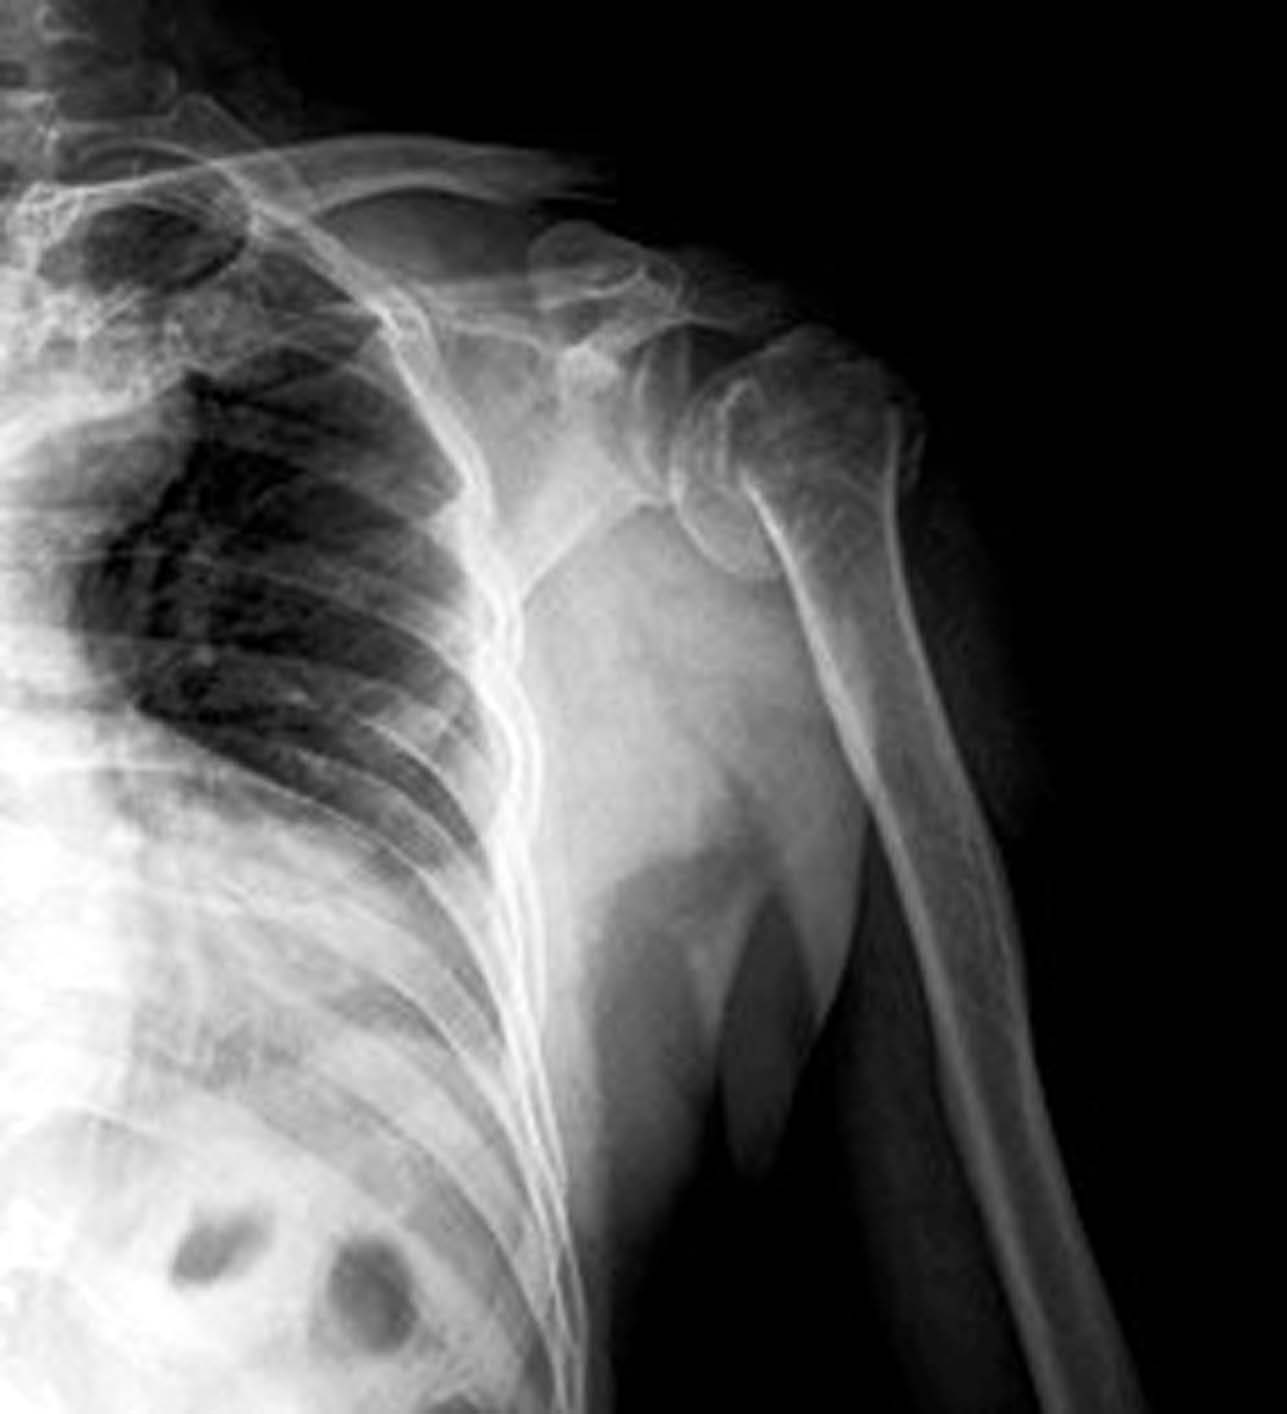
\includegraphics{./images/Image00030.jpg}
 \captionsetup{justification=centering}
 \caption{肩关节正位}
 \label{fig2-3-3}
  \end{figure} 

\textbf{【病史摘要】}
 男性,73岁。跌倒时左肩部外展着地,肿痛,活动受限。

\textbf{【X线表现】}
 左肱骨外科颈处见骨折线,肱骨头向下倾斜,远断端向上移位,外侧见小骨片。

\textbf{【X线诊断】}  肱骨外科颈骨折(内收型)。

\textbf{【评  述】}
 肱骨外科颈位于解剖颈下方2~3cm,是肱骨头松质骨和肱骨干皮质骨交界的部位,易发生骨折。各种年龄均可发生,老年人较多。X线片可确诊,且可显示骨折类型及移位情况。区分外科颈骨折的类型是影像检查的主要目的,主要分为三型:①内收或外展型损伤:最常见。X线正位片所见骨折线为横行,骨折轻度向内或向外成角,远侧断端内收或外展。侧位片上均无明显向前或向后成角、错位改变。②伸展型损伤:是间接外力引起的损伤。X线特点为骨折线横行,骨折向前成角,远侧断端向前错位,肱骨头后倾,关节面向后。③屈曲型损伤:是较少见的间接外力引起的损伤。骨折向后成角畸形,远侧断端向后上移位。

\subsection{肱骨髁上骨折}

\begin{figure}[!htbp]
 \centering
 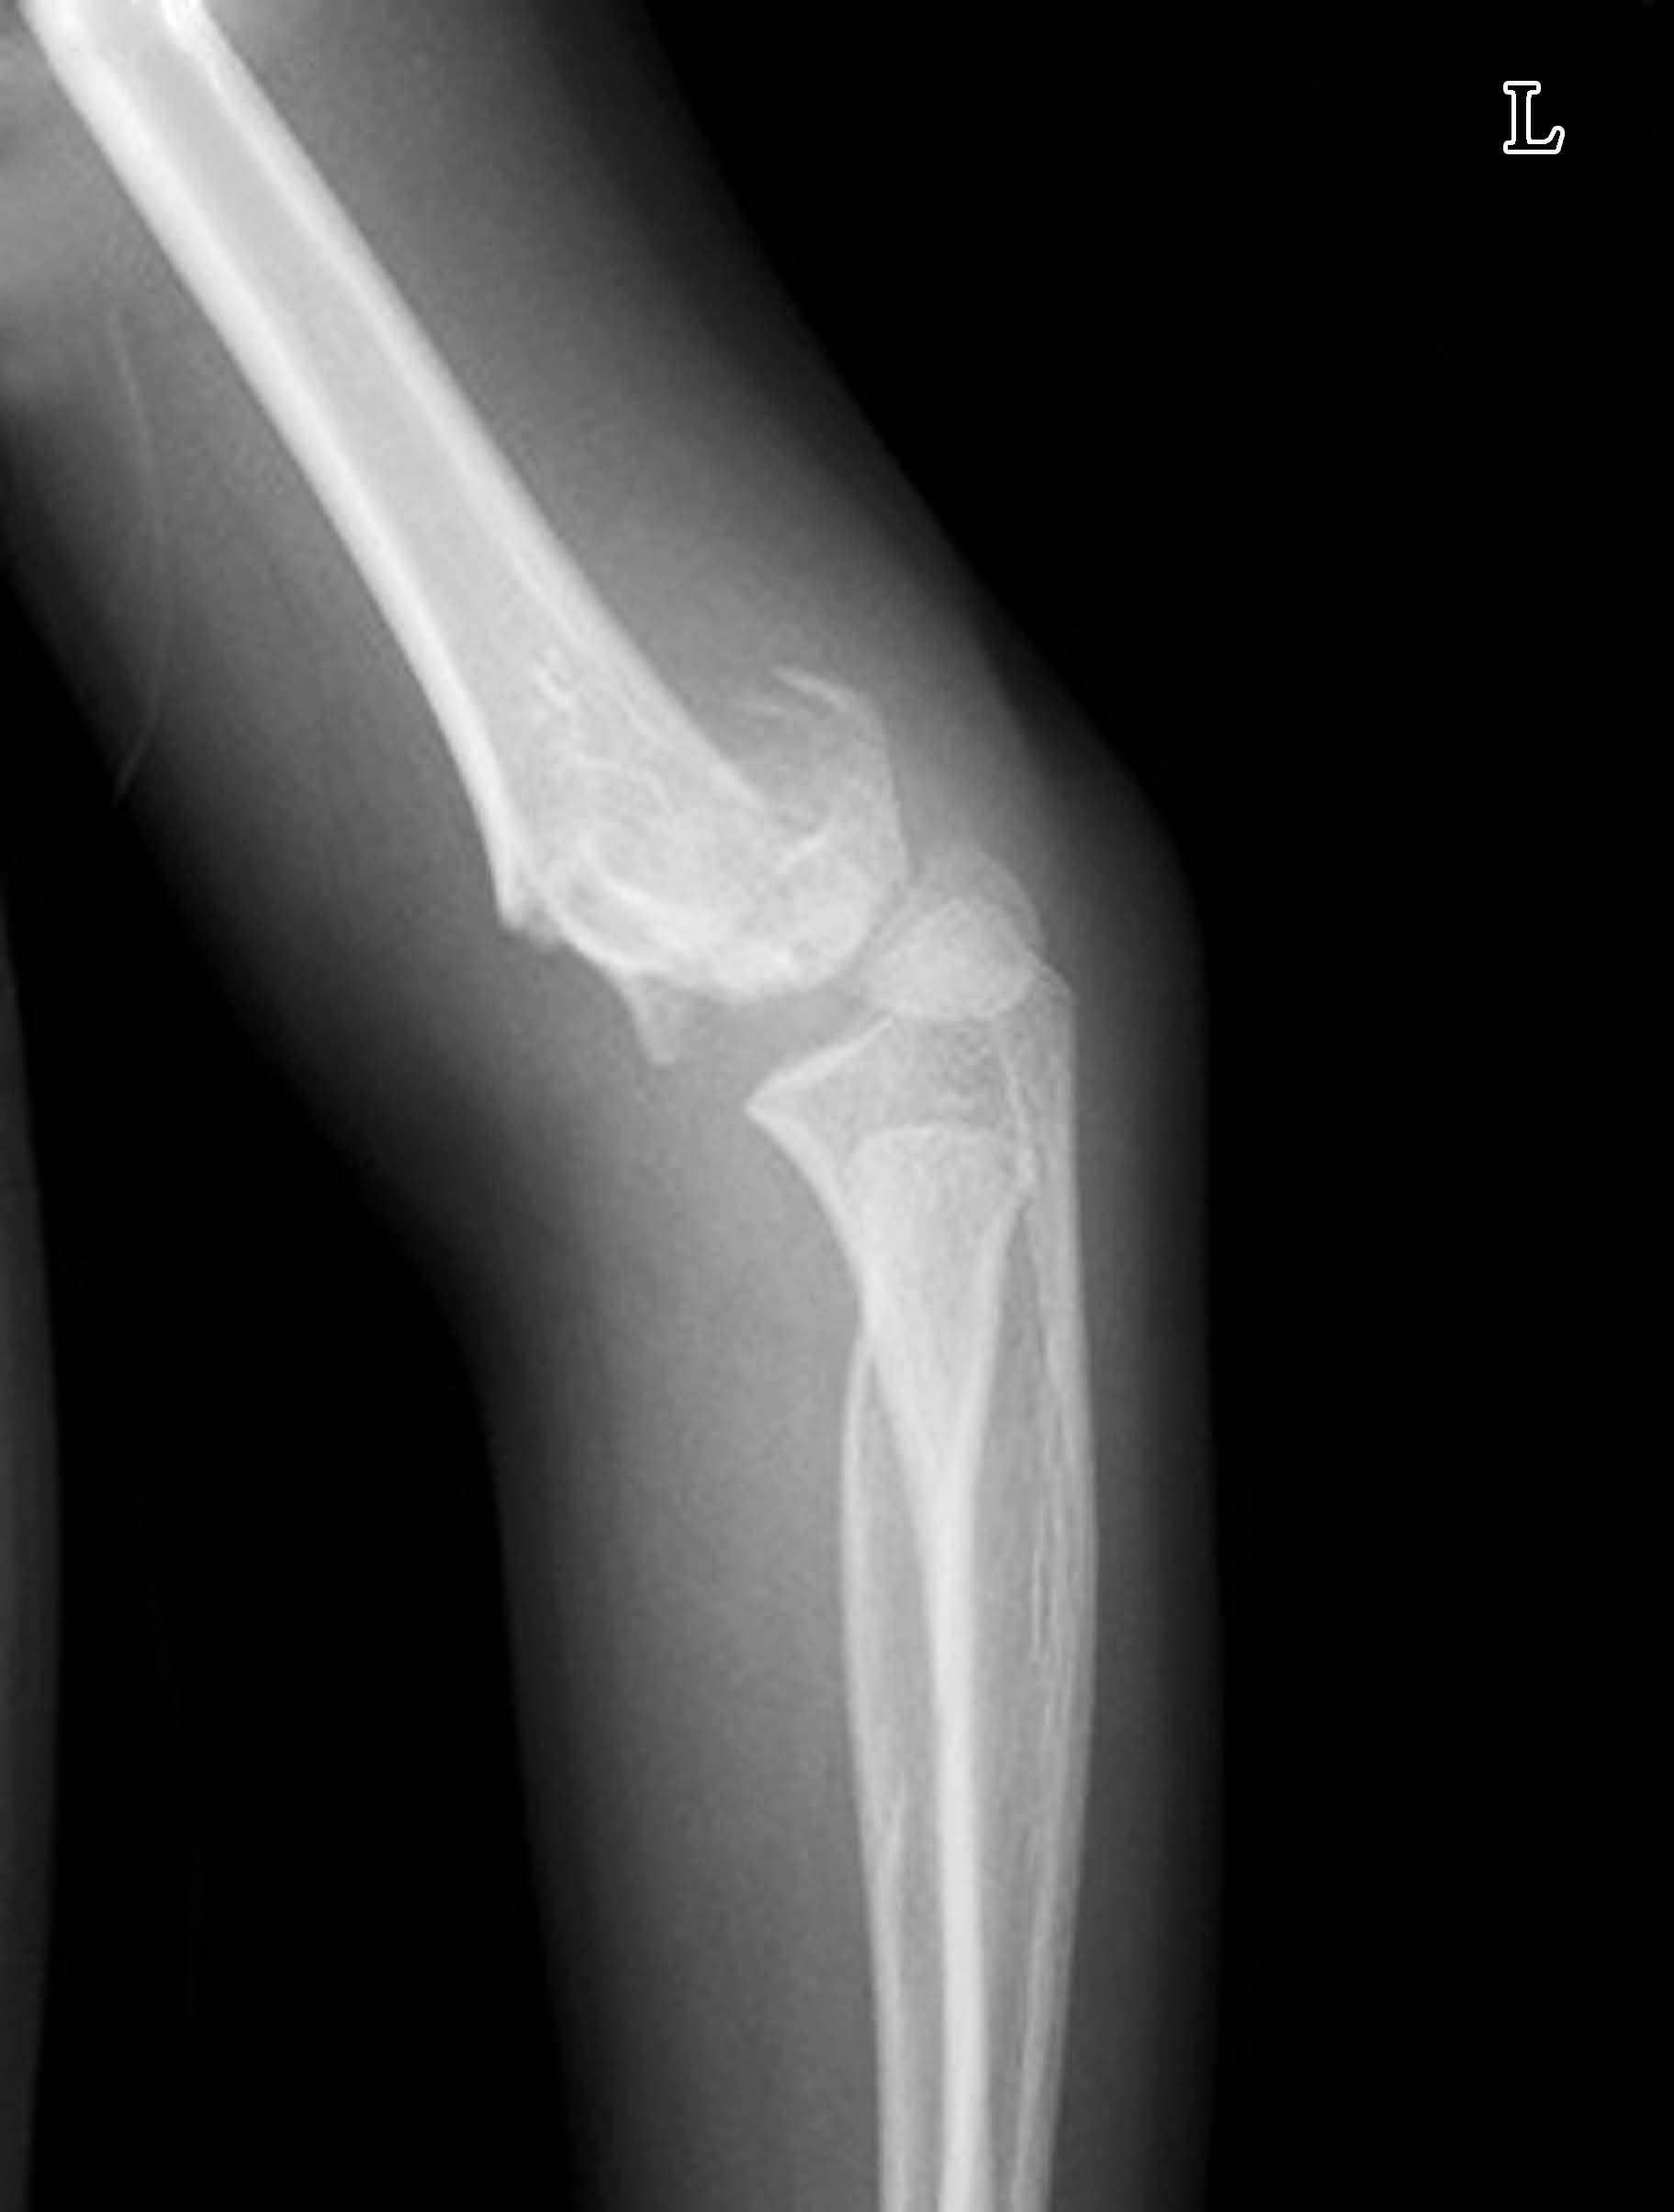
\includegraphics{./images/Image00031.jpg}
 \captionsetup{justification=centering}
 \caption{肘关节侧位}
 \label{fig2-3-4}
  \end{figure} 

\textbf{【病史摘要】}
 男性,8岁。跌倒时左手臂伸直,手掌着地。左肘关节肿胀、畸形、活动障碍。

\textbf{【X线表现】}  左肱骨髁上见横行骨折线,骨折远断端向背侧移位。

\textbf{【X线诊断】}  左肱骨髁上骨折(伸直型)。

\textbf{【评  述】}
 肱骨髁上骨折,最多见于儿童,成人及老年人亦可发生,是肘部最常见的损伤。髁上骨折基本分为两型:①伸展型损伤,儿童最多见,占此型90%以上。骨折线通过鹰嘴窝或其上方,骨折线由前下至后上,断端间向前成角,骨折断端向后上方移位。②屈曲型损伤,见于较大儿童、成人或老年人,较少见,仅占8%。骨折线亦位于髁上,多呈斜行,由后下向前上或者横断,断端间向后成角,骨折远端向前移位。肱骨髁上骨折应注意和肱骨远端全骺分离相鉴别。骨骺全分离在X线片无骨折线,桡骨纵轴线与肱骨小头关系不变,但与肱骨下端关系改变,肘部肿胀,环周压痛。

肘部是外伤常见的部位,特别是儿童,由于肘部解剖结构比较复杂,有时比较严重的创伤在X线上可能仅表现为轻微异常。以下几点可帮助鉴别肘部创伤:①骨化中心的判定,骨化中心最常见的顺序为CRITOL,即肱骨小头(Capitellum,C),桡骨小头(Radical head,RI),滑车(Trochlea,T),鹰嘴(Olecranon,O),外上髁(Lateral epicondyle,L),熟悉骨化中心出现的顺序便可与异常的骨折碎骨片相鉴别;②脂肪垫征;③肱骨前线,正常侧位片上沿肱骨皮质前缘画一条线,与肱骨小头前中1/3相交,如果肱骨小头前缘位置超过肱骨前线不足1/3,则提示髁上骨折并远侧断端后移;④桡肱小头线,沿近端桡骨干的中心画线并经过肱骨小头中心,称为桡肱小头线,若该线未经过肱骨小头,则提示桡骨小头或肱骨小头移位。

\subsection{肱骨髁间骨折}

\begin{figure}[!htbp]
 \centering
 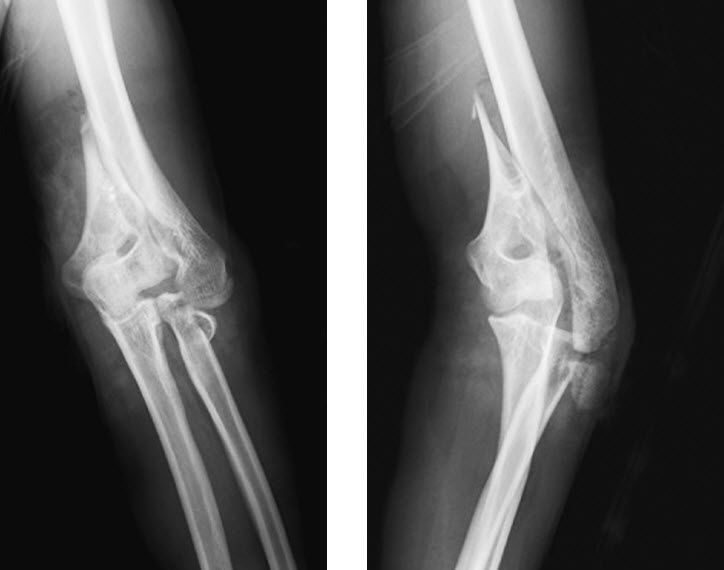
\includegraphics{./images/Image00032.jpg}
 \captionsetup{justification=centering}
 \caption{肘关节正侧位}
 \label{fig2-3-5}
  \end{figure} 

\textbf{【病史摘要】}  男性,29岁。车祸伤及左肘,肿痛、活动障碍。

\textbf{【X线表现】}
 左肱骨髁间见斜行骨折线,远断端略向上移位;左桡骨小头骨折、移位。

\textbf{【X线诊断】}  左肱骨髁间骨折;左桡骨小头骨折。

\textbf{【评  述】}
 肱骨髁间骨折,多见于成人,是肘部较严重的关节内骨折,较少见。骨折线从肱骨两髁之间纵行向上,把两髁劈裂为两半,整个骨折线可呈T形或Y形。肱骨髁间骨折有时需与肱骨髁上骨折相鉴别。前者骨折波及关节面,关节面破坏;后者未波及关节面。

一份合格的骨折平片及X线诊断报告需要向临床提供四方面的信息:①解剖位置(定位);②骨折的类型(横形骨折、斜形骨折、螺旋形骨折,闭合性骨折、开放性骨折,关节外骨折、关节内骨折,病理性骨折,青枝骨折等);③骨折两端的对位、对线关系;④软组织损伤评价。

\subsection{尺骨鹰嘴骨折}

\begin{figure}[!htbp]
 \centering
 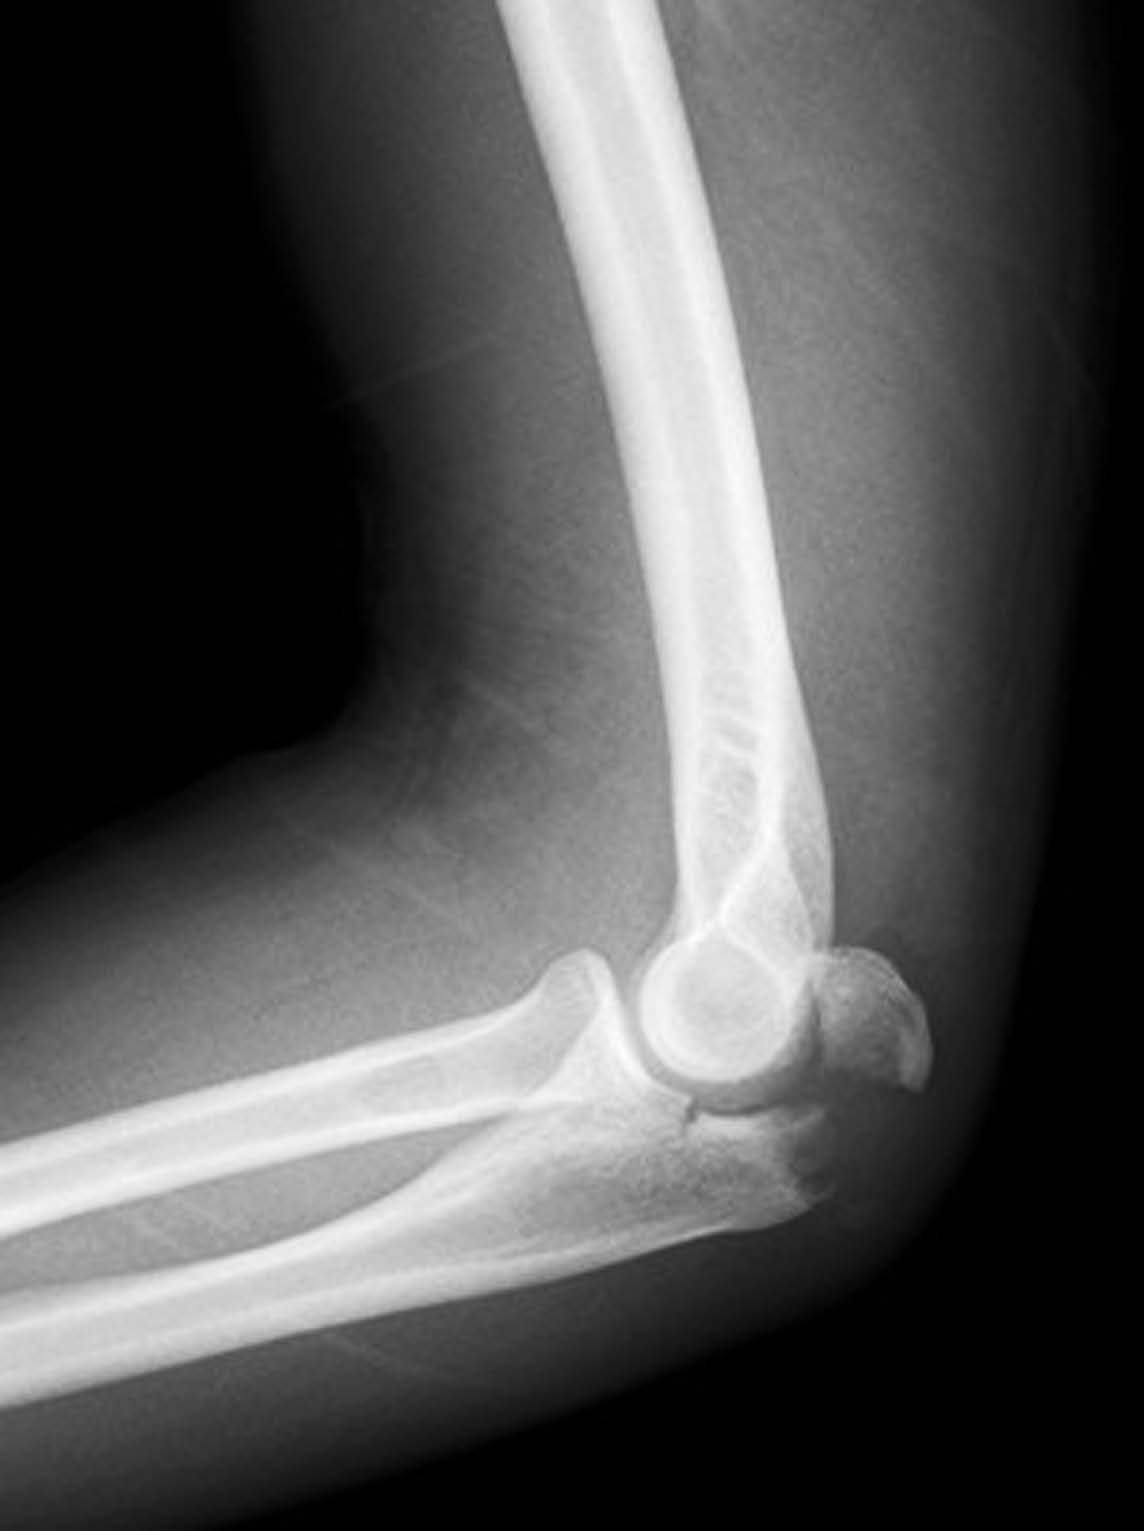
\includegraphics{./images/Image00033.jpg}
 \captionsetup{justification=centering}
 \caption{肘关节侧位}
 \label{fig2-3-6}
  \end{figure} 

\textbf{【病史摘要】}  男性,51岁。骑车摔伤右肘部,疼痛,活动障碍。

\textbf{【X线表现】}  右尺骨鹰嘴处见骨折线,断端分离。

\textbf{【X线诊断】}  右尺骨鹰嘴骨折。

\textbf{【评  述】}
 尺骨鹰嘴骨折常由肘部直接暴力所致,多为粉碎性骨折。骨片移位较少。尺骨鹰嘴为肱三头肌的止点,当肱三头肌急骤收缩使肘关节伸直时,而另一暴力强使其屈曲,易造成尺骨鹰嘴撕脱性骨折,骨片可很小,也可是近端骨折被牵拉而向上移位。本例考虑病因为后者。肘关节骨化中心在融合前有可能与骨折混淆,可疑者应摄健侧X线片以行对比。

脂肪垫征(或后脂肪垫征、前脂肪帆征)对儿童的肘关节损伤检查有帮助,常提示肘关节骨折,主要见于髁上骨折、侧髁骨折和桡骨小头骨折。存在脂肪垫则应立即寻找这些骨折。在标准屈肘侧位片上,常可见到前侧脂肪垫,而不能见到后侧脂肪垫。肘关节内的渗出能使前后侧脂肪垫都增厚且在同一张肘侧位X线片上观察到。肘关节伤后出现增厚的后侧脂肪垫征提示有肘关节囊内骨折的可能。以往报道侧位X线片上显示后侧脂肪垫增厚者有明显囊内骨折的占41%~100%。因此,即使未见骨折亦应夹板固定、随访。

\subsection{Monteggia骨折}

\begin{figure}[!htbp]
 \centering
 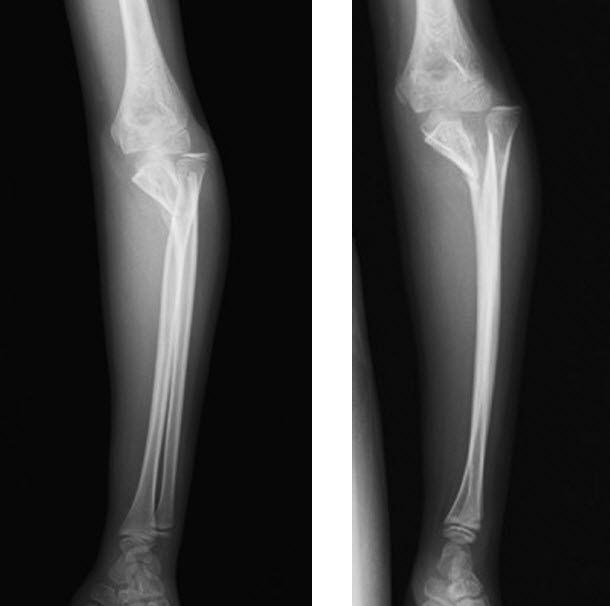
\includegraphics{./images/Image00034.jpg}
 \captionsetup{justification=centering}
 \caption{尺桡骨斜位、侧位}
 \label{fig2-3-7}
  \end{figure} 

\textbf{【病史摘要】}
 男性,13岁。跌倒时左肘微屈,前臂旋前着地。左肘部肿胀,疼痛,功能障碍。

\textbf{【X线表现】}
 左尺骨近段骨折,断端向背侧成角;桡骨小头向后外侧脱位。

\textbf{【X线诊断】}  左前臂Monteggia骨折(屈曲型)。

\textbf{【评  述】}
 Monteggia骨折,是指尺骨近段骨折合并桡骨小头脱位。本病多发生于青壮年及小儿,直接或间接暴力皆可引起。根据暴力方向及移位情况临床可分为伸直型、屈曲型和内收型。前臂正位、侧位片可以确诊。摄片时应包括肘关节以免漏诊,同时注意肱桡关节的解剖关系,必要时可加摄健侧X线片做对照。本病主要与先天性桡骨头脱位鉴别。后者缺乏外伤病史,多为双侧,多伴有桡骨头发育畸形等。

\subsection{肘关节后脱位}

\begin{figure}[!htbp]
 \centering
 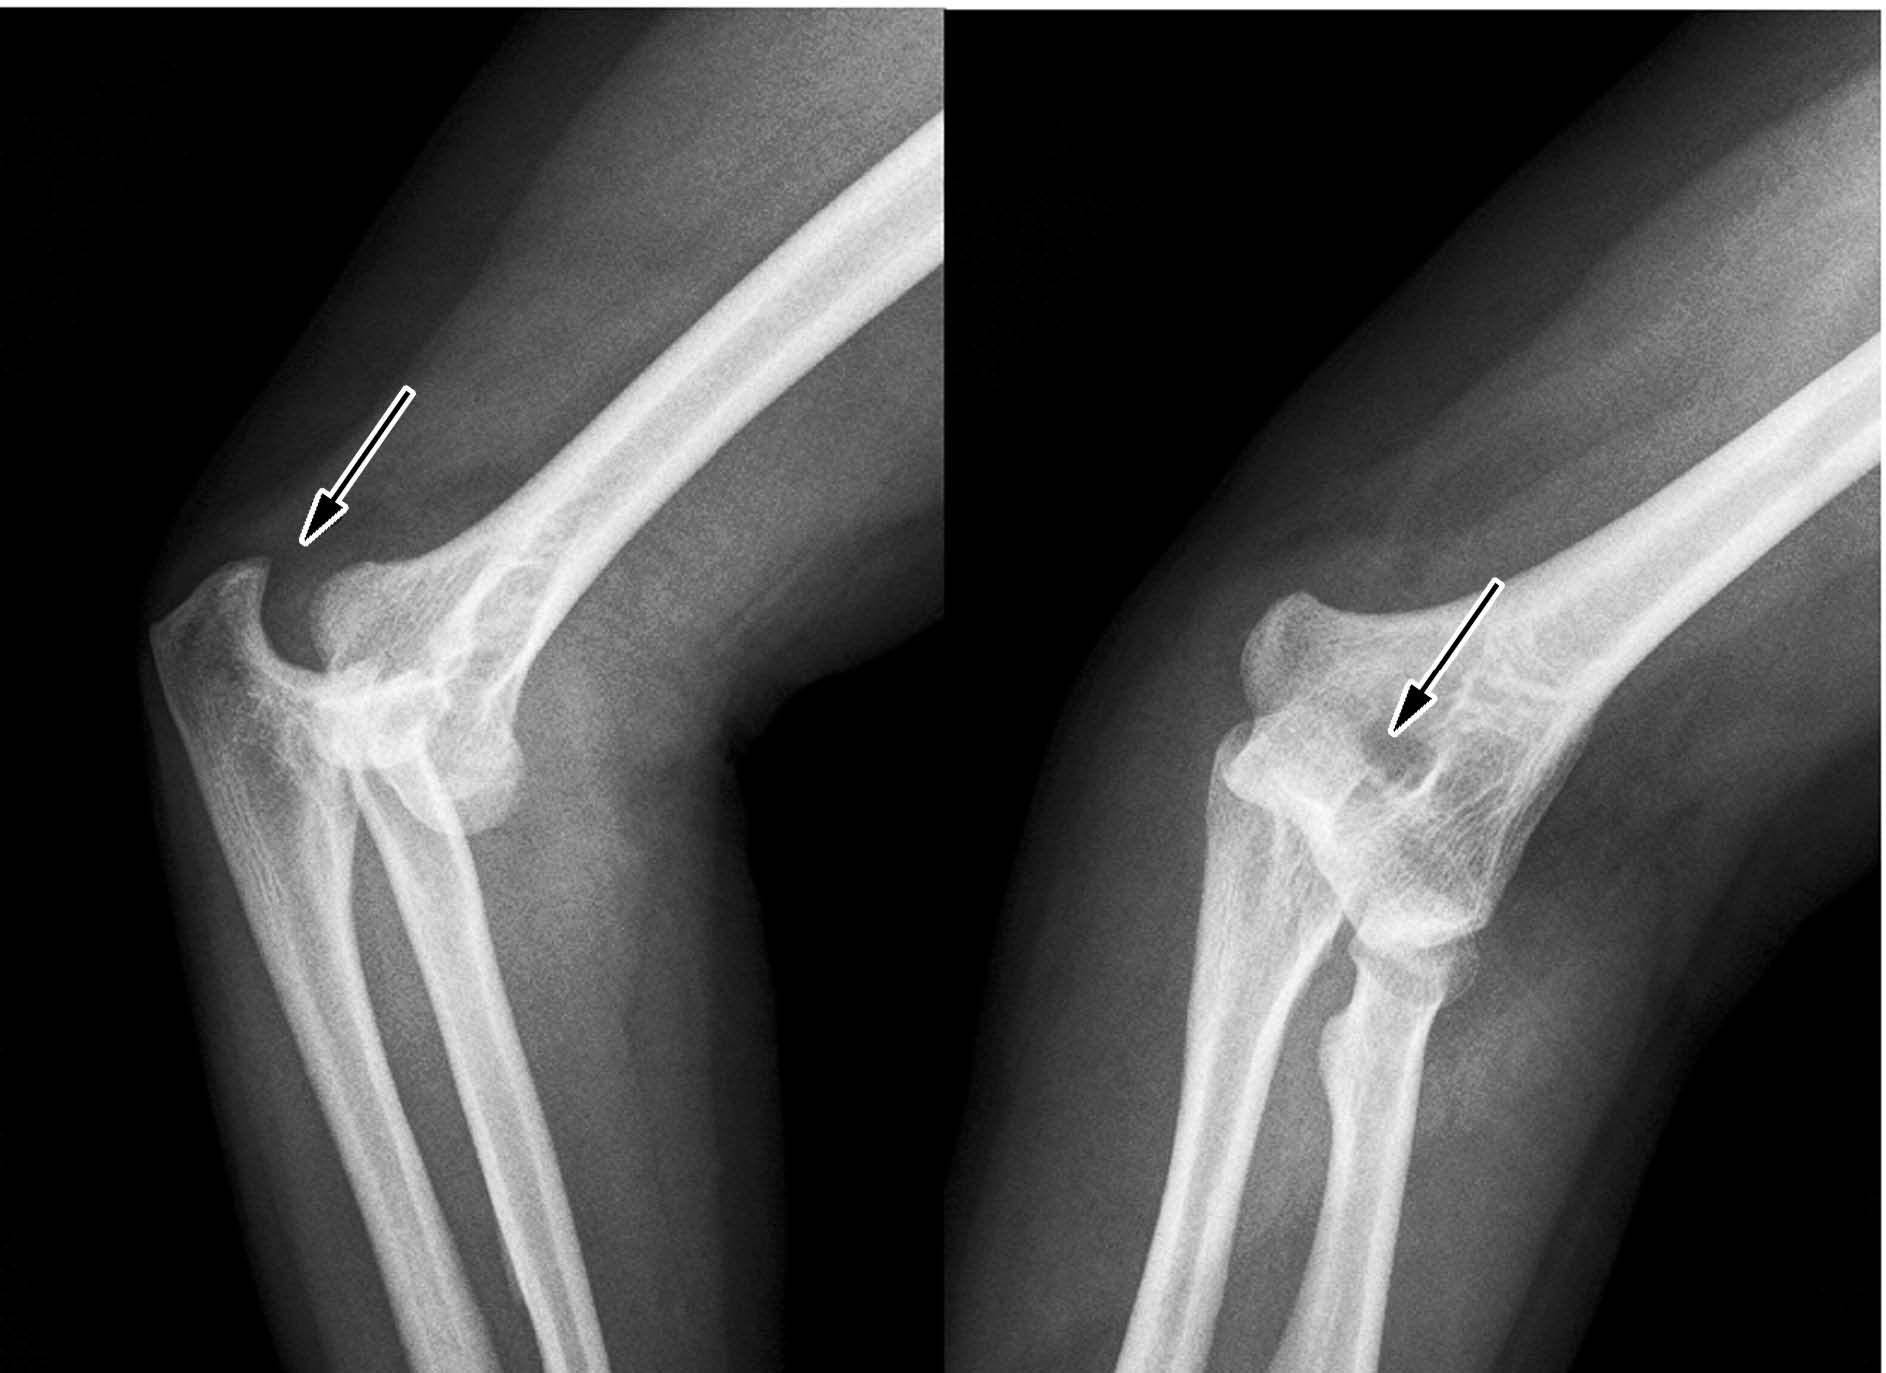
\includegraphics{./images/Image00035.jpg}
 \captionsetup{justification=centering}
 \caption{肘关节正侧位}
 \label{fig2-3-8}
  \end{figure} 

\textbf{【病史摘要】}
 女性,47岁。跌倒时右肘关节伸直,右手掌撑地,关节畸形,活动障碍。

\textbf{【X线表现】}  右尺桡骨近端向后外方移位,关节结构紊乱(箭头)。

\textbf{【X线诊断】}  右肘关节后脱位。

\textbf{【评  述】}
 肘关节脱位是四肢关节中最多见的一种脱位,肘部畸形呈弹性固定状,鹰嘴窝空虚,常合并骨折,或伴有血管、神经损伤。X线正位片见尺桡骨上端与肱骨下端重叠,肘关节间隙消失。侧位见桡骨头与尺骨鹰嘴向后移位,有时两者可同时向外或内侧移位,肱尺、肱桡关节对应关系失常,常伴有尺骨鹰嘴、滑车后缘、肱骨内上髁或外上髁等骨折。临床治疗前需鉴别后脱位和前脱位:前者,暴力传导到肘部后上方,沿尺骨纵轴上传,鹰嘴突撞击肱骨下端鹰嘴窝,将关节囊撕裂,尺骨冠状突和桡骨小头同时滑向后方;后者,前臂遭受自肘后方向前或纵向扭转的暴力,可致鹰嘴骨折,尺桡骨上段向前移至肱骨下端前方。

\subsection{桡骨远端伸直型骨折}

\begin{figure}[!htbp]
 \centering
 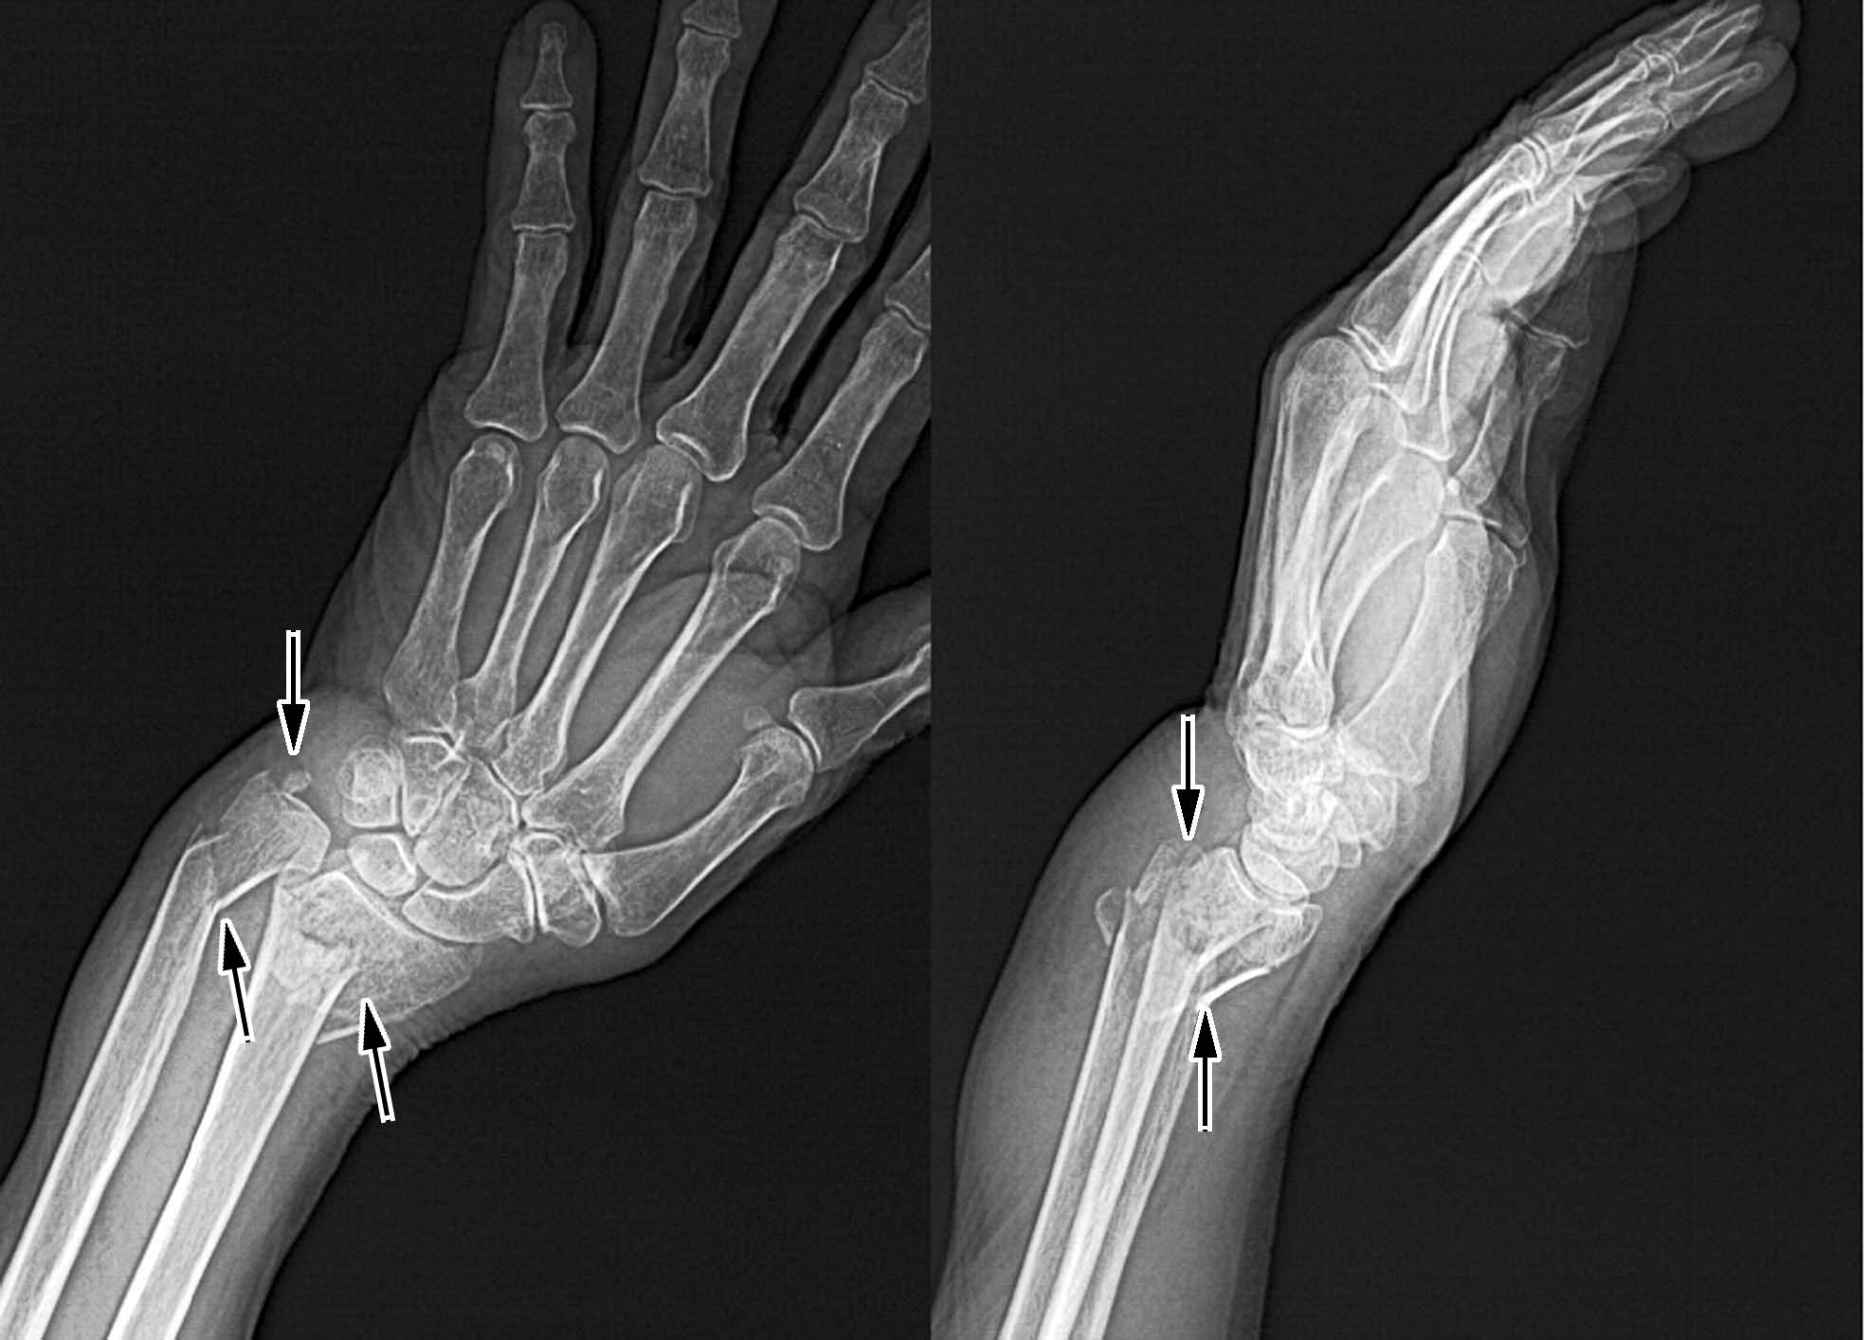
\includegraphics{./images/Image00036.jpg}
 \captionsetup{justification=centering}
 \caption{腕关节正侧位}
 \label{fig2-3-9}
  \end{figure} 

\textbf{【病史摘要】}
 女性,62岁。被撞倒时右手掌着地,右腕关节畸形、肿胀,不能活动。

\textbf{【X线表现】}
 右尺桡骨远端见透亮线影,骨折远端向外后方移位,尺骨茎突见小骨片影(箭头)。

\textbf{【X线诊断】}  右桡骨远端伸直型骨折(Colles骨折)。

\textbf{【评  述】}
 Colles骨折最常见于老年女性,为发生在桡骨远端、距离远端关节面2.5cm内的横行骨折,骨折可累及桡腕关节及下尺桡关节,引起脱位或半脱位,约60%伴尺骨茎突骨折,其特征性的临床表现为手腕呈银叉状畸形。Colles骨折需与Smith骨折鉴别:前者为摔倒时手掌着地所致,常伴远侧断端向桡背侧移位和向掌侧成角;后者即桡骨远端屈曲型骨折,为跌倒时手背着地所致,远侧断端向掌侧上方移位和向背侧成角,也称反Colles骨折。

\subsection{桡骨远端骨骺分离}

\begin{figure}[!htbp]
 \centering
 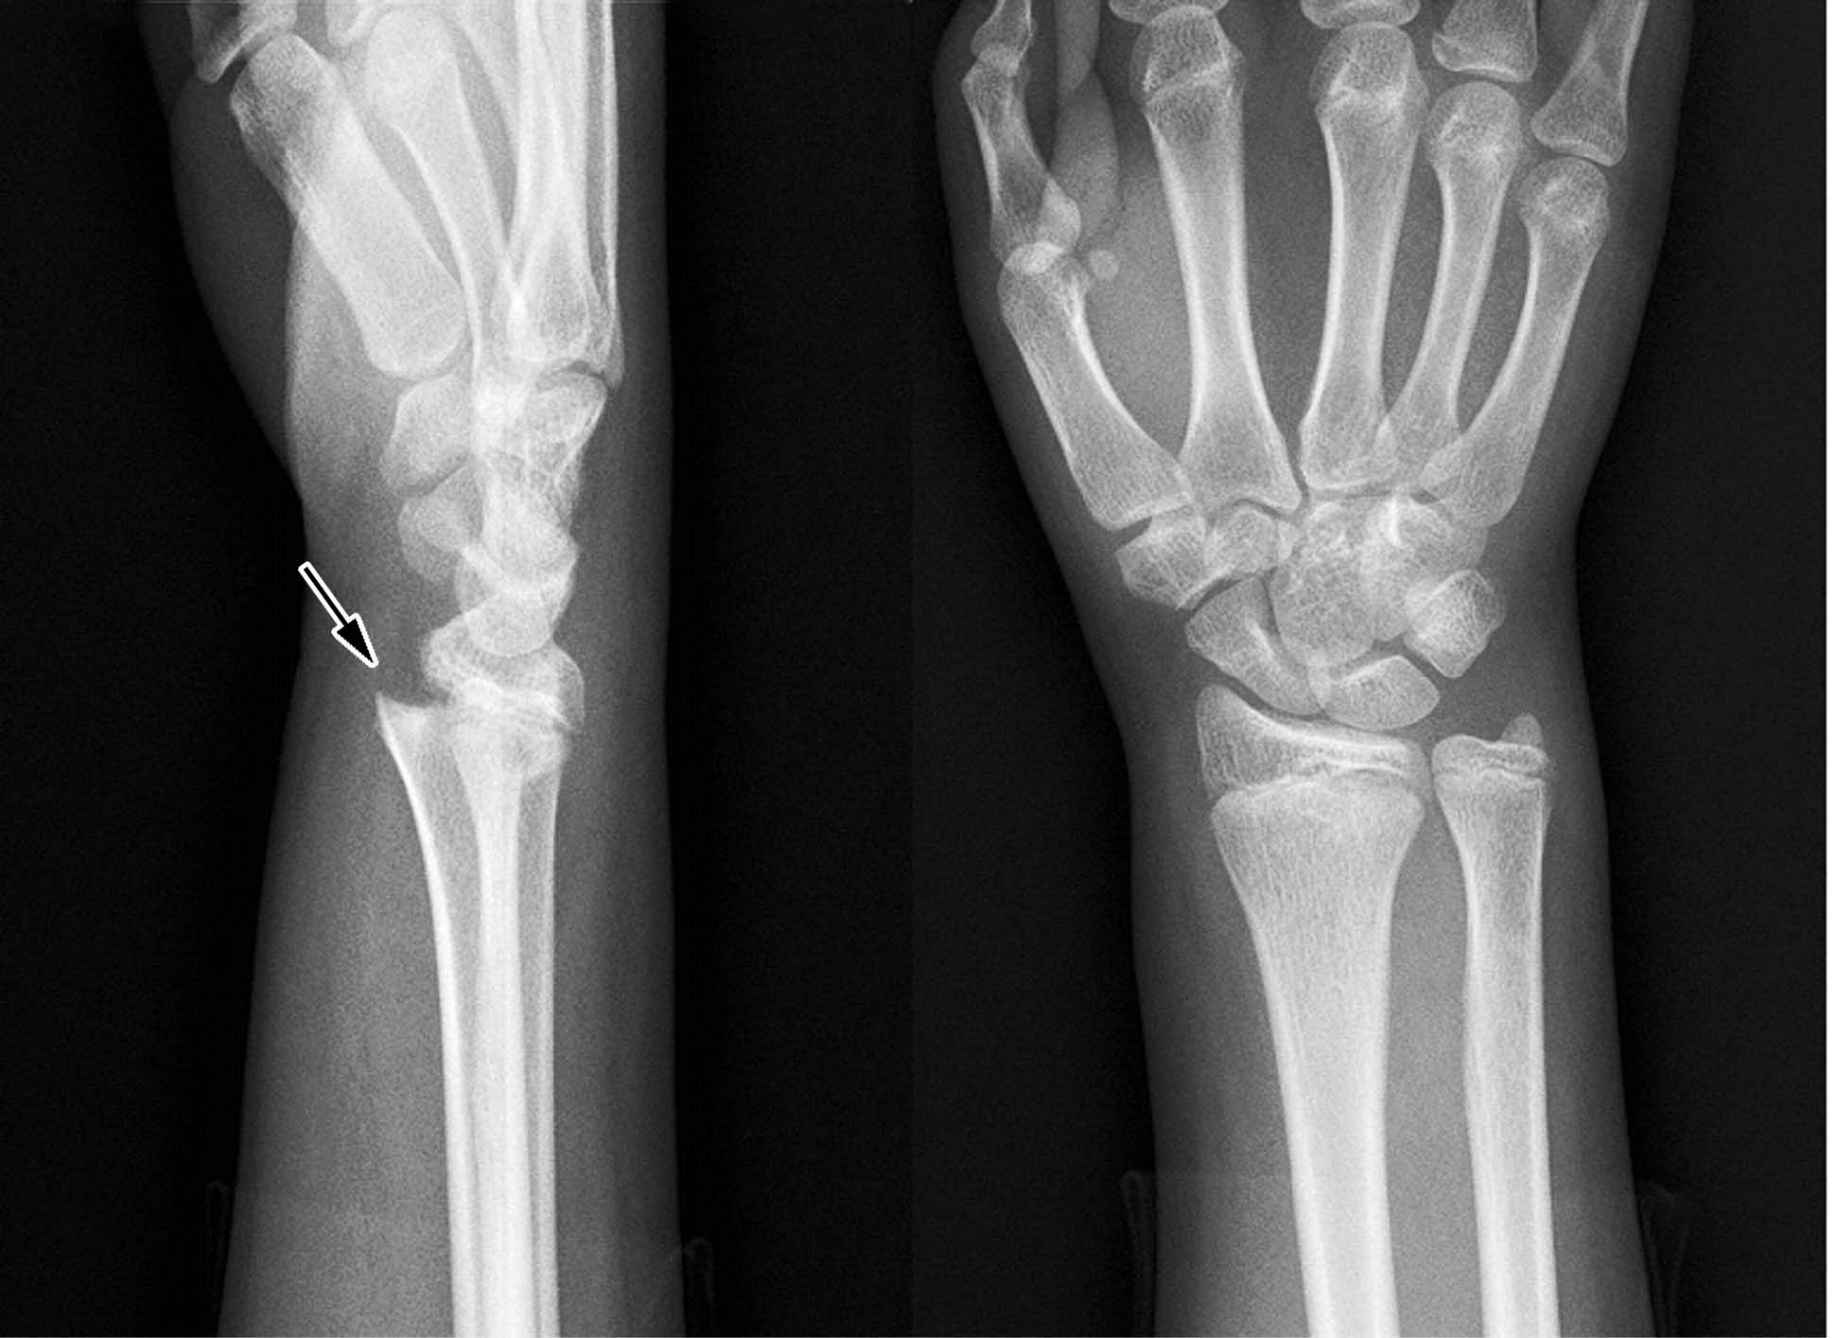
\includegraphics{./images/Image00037.jpg}
 \captionsetup{justification=centering}
 \caption{腕关节正侧位}
 \label{fig2-3-10}
  \end{figure} 

\textbf{【病史摘要】}  女性,12岁。撞倒时左手掌着地,左腕关节活动障碍。

\textbf{【X线表现】}
 侧位片示左桡骨远端骨骺向后移位,关节面成轻度后倾角畸形改变(箭头);正位片未见明显异常。

\textbf{【X线诊断】}  左桡骨远端骨骺分离。

\textbf{【评  述】}
 骨骺分离是儿童骨关节损伤中最常见的,所有四肢管状骨骨骺均可发生,其创伤机制是垂直和水平两个方向的综合暴力造成的,不熟悉儿童骨骺发育及解剖情况,极易造成漏诊,应着重观察侧位片。根据X线表现,骨骺损伤分为五种类型(Salter-Harris分类法):Ⅰ型,骨骺与干骺端完全分离,骨折线完全通过骺板的薄弱带;Ⅱ型,部分骺板断裂,可以有干骺端小的骨折片仍与骨骺相连,但干骺端的主要部分与骨骺分离,此型最为多见;Ⅲ型,骨折线自关节面进入骨骺达骺板处再沿一侧薄弱带到骨骺板边缘;Ⅳ型,骨折线穿过干骺端、骺板和骨骺的骨折,多数也穿过关节软骨;Ⅴ型,骨骺软骨板的压缩性骨折,临床症状明显,但查不出明显骨骺损伤时,要考虑到本型。

青少年骨骺发育不全,骺板(生长板)相对脆弱,容易受到损伤。骨骺/干骺骨折分离可导致骨骺早闭的并发症。若患者临床症状明显但X线检查未发现异常时,可行MRI检查以明确骨骺损伤的类型和程度。

\subsection{桡骨远端青枝骨折}

\begin{figure}[!htbp]
 \centering
 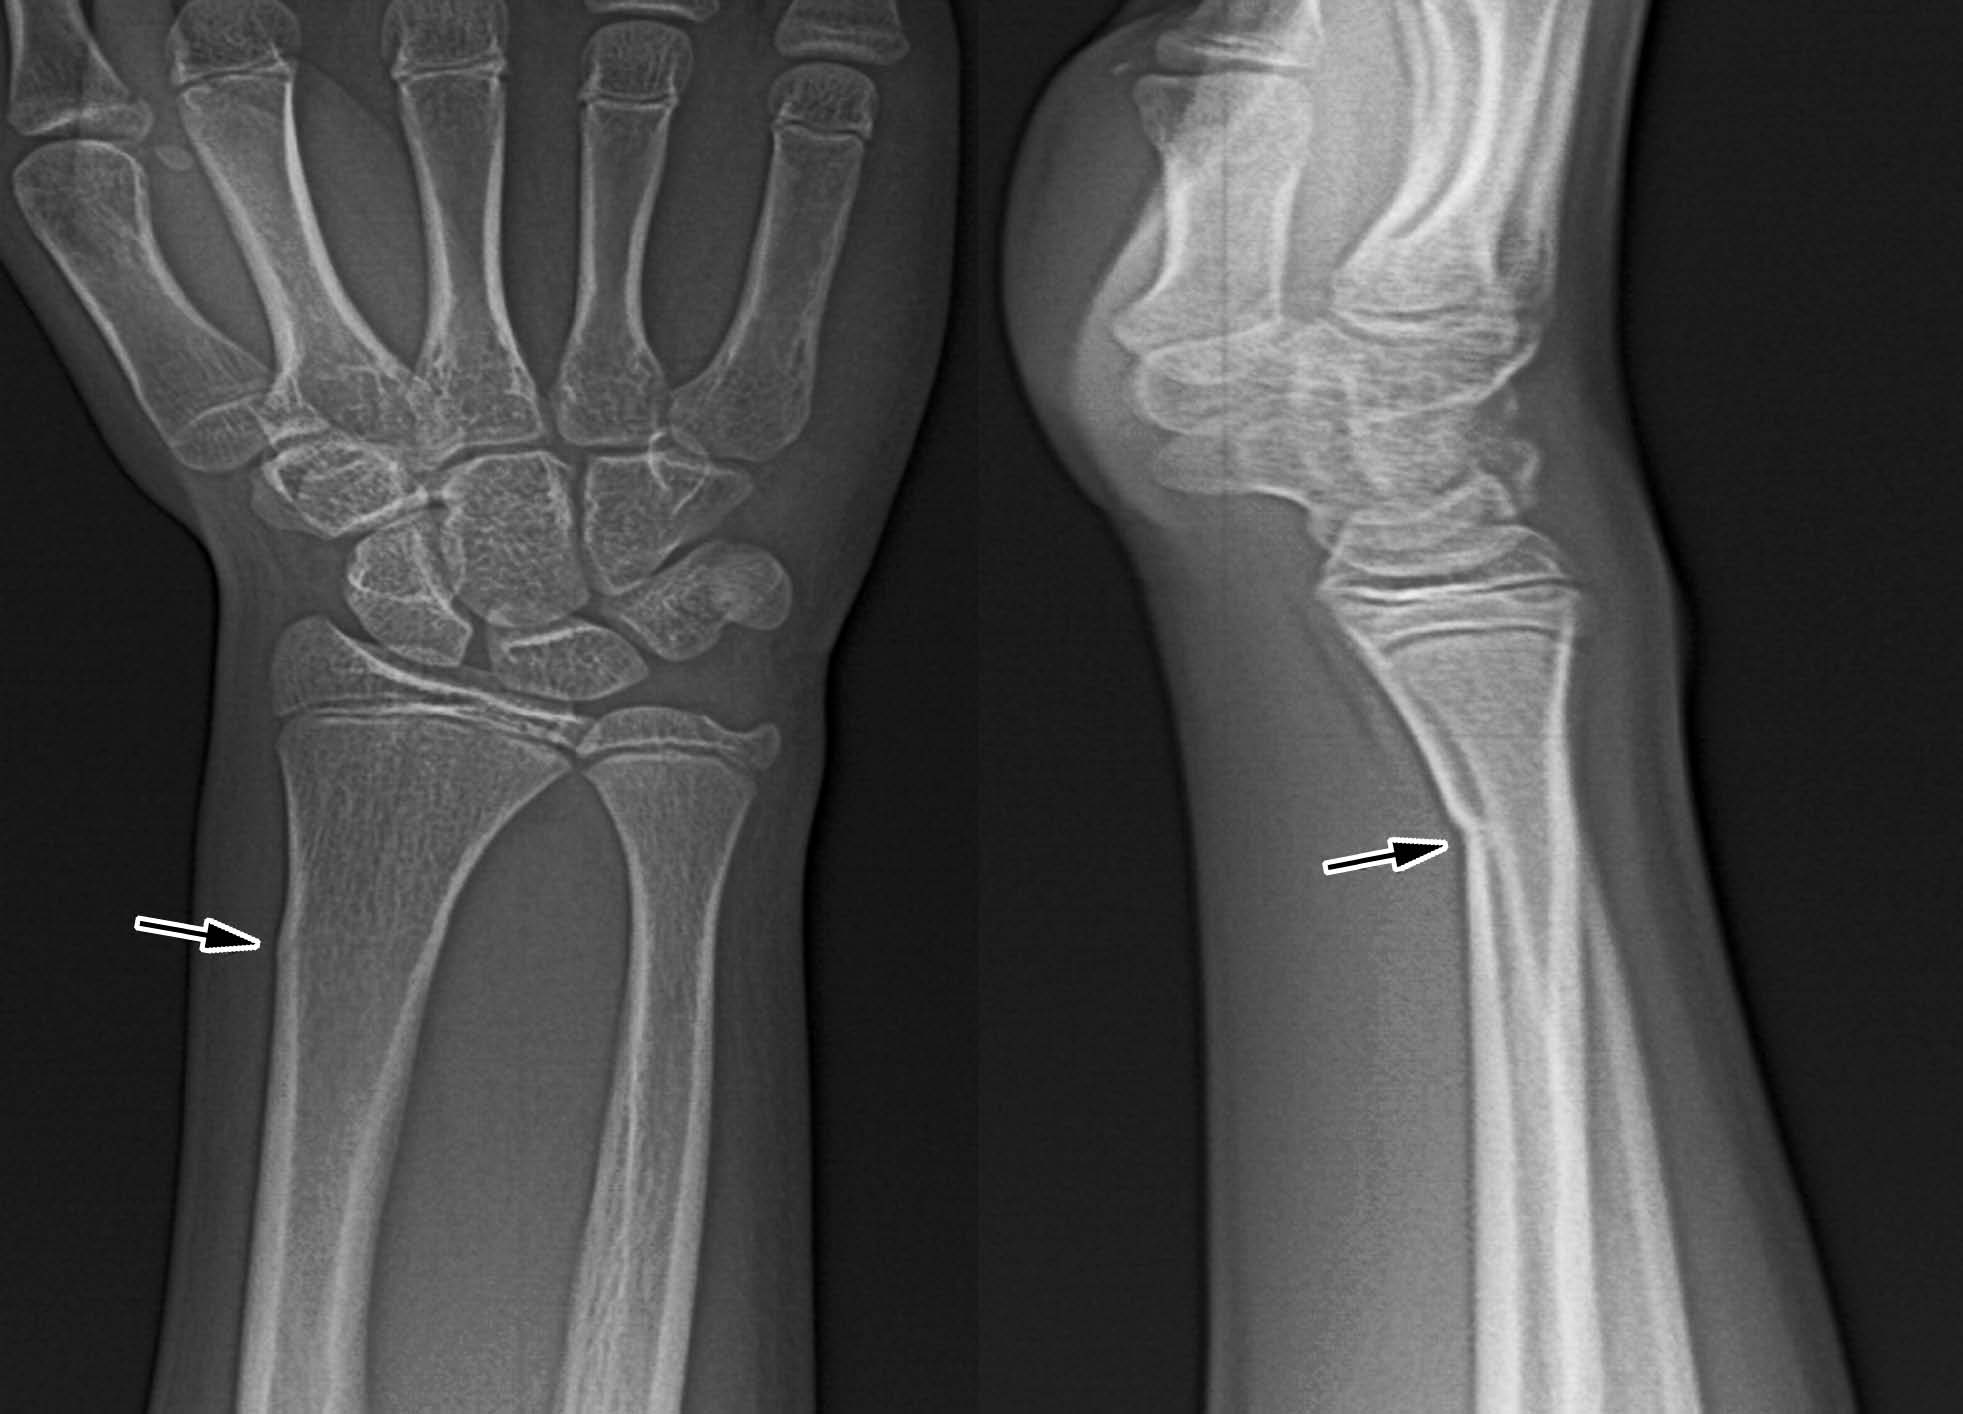
\includegraphics{./images/Image00038.jpg}
 \captionsetup{justification=centering}
 \caption{腕关节正侧位}
 \label{fig2-3-11}
  \end{figure} 

\textbf{【病史摘要】}  男性,9岁。跌倒时右手腕着地,手腕疼痛。

\textbf{【X线诊断】}
 右桡骨远端骨皮质皱褶,骨折断端轻微成角畸形(箭头)。

\textbf{【X线表现】}  右桡骨远端青枝骨折。

\textbf{【评  述】}
 青枝骨折多见于儿童,儿童的骨骼在力学上具有很好的弹性和韧性,遭受暴力发生骨折就会出现与植物青枝一样折而不断的情况,属于稳定性骨折,通常不需要手术治疗。需与完全性骨折相鉴别。青枝骨折表现为桡骨张力侧骨皮质发生皱褶、扭曲、断端轻微成角,为不完全性骨折;后者表现为骨皮质完全断裂,骨折线呈横形、纵形、斜形或螺旋形等,断端常移位。

儿童骨质富有弹性和柔韧性,不易碎裂,故其特点与成人不同。常见的儿童骨折有以下几种类型:青枝骨折、带扣样骨折、管状骨折、弓形骨折、婴儿骨折、骨骺/干骺骨折、撕脱性骨折以及完全性骨折。带扣样骨折指外力冲击或压迫导致骨皮质隆起呈带扣样改变,常见于长骨,尤其是尺桡骨的干骺端。管状骨折是一侧骨皮质不完全性横断骨折,对侧皮质呈带扣样骨折。弓形骨折指长骨的弓形弯曲,一般无骨折,但可伴发毗邻骨的骨折,好发于尺桡骨及腓骨等。婴儿骨折一般无明确外伤史,但见于跛行的幼儿。多为行X线检查意外发现的无移位的骨折。最早见于胫骨远端,也可见于股骨远端及跟骨。撕脱性骨折多发生于韧带或肌腱附着处,可见于任何年龄。青年的次级骨化中心(骨突)尤其是骨盆最易发生撕脱性骨折。

\subsection{腕手舟骨骨折}

\begin{figure}[!htbp]
 \centering
 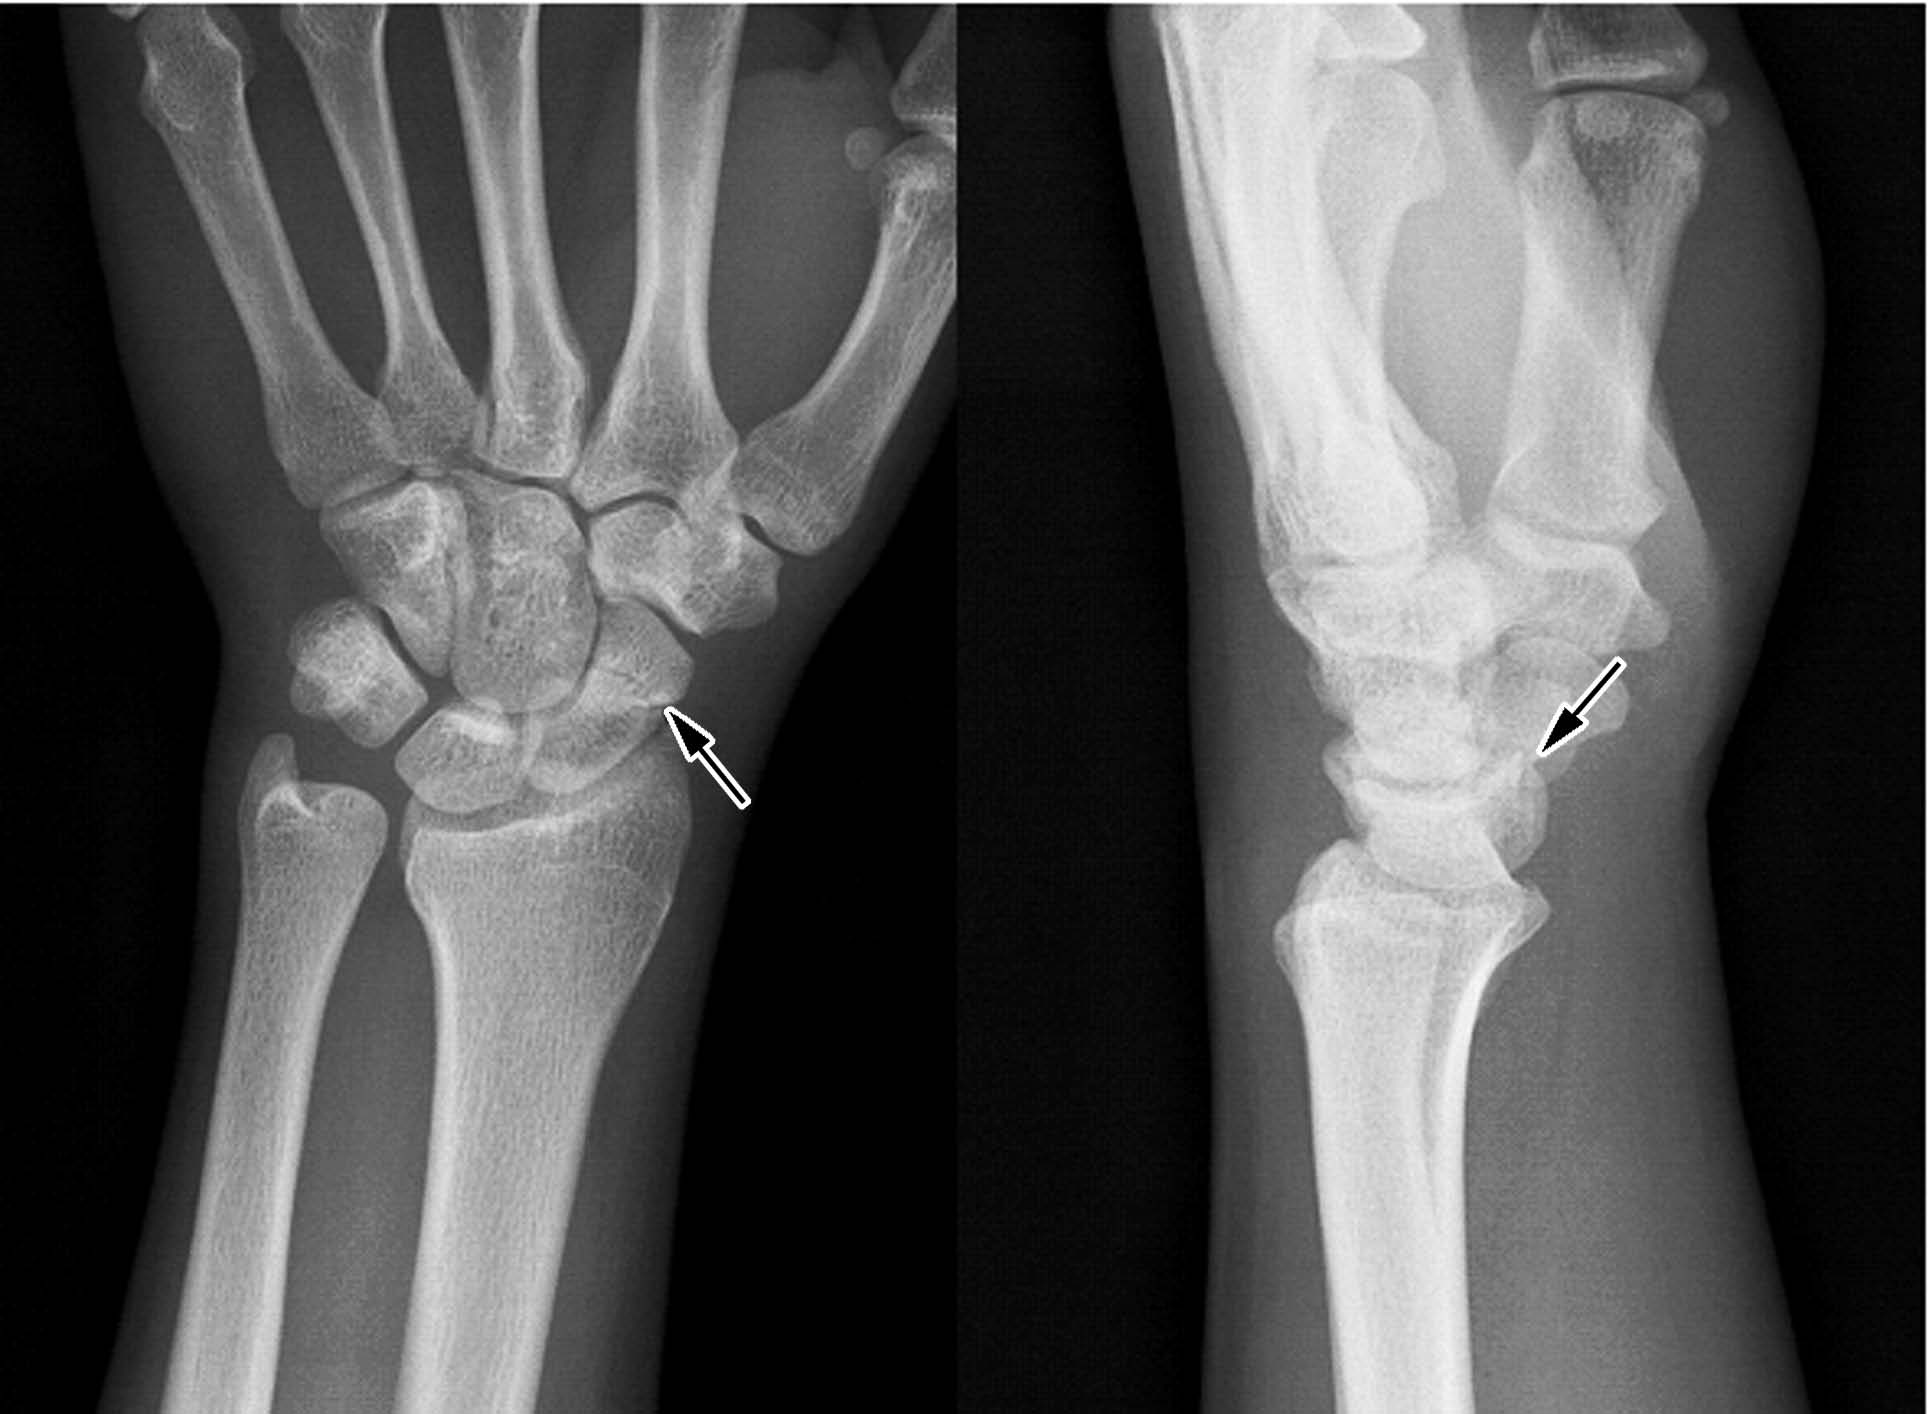
\includegraphics{./images/Image00039.jpg}
 \captionsetup{justification=centering}
 \caption{腕关节正侧位}
 \label{fig2-3-12}
  \end{figure} 

\textbf{【病史摘要】}
 男性,30岁。撞倒时左手掌着地,鼻咽窝变浅、压痛,左腕关节背伸时压痛明显。

\textbf{【X线表现】}  左手腕手舟骨上腰部见透亮线影,对位好(箭头)。

\textbf{【X线诊断】}  左腕手舟骨骨折。

\textbf{【评  述】}
 腕骨损伤以手舟骨最多见,三角骨和月骨次之,其创伤机制为跌倒时手掌着地后传达暴力直接作用于手舟骨发生骨折,多见腰部,结节部较少见,因血供差,易引起骨迟缓愈合和不愈合,甚至发生缺血坏死。临床怀疑手舟骨骨折时,应摄腕关节外展位(手舟骨位)片,一次摄片未发现,则应在7~10天后复查,此时骨折线附近的骨质吸收,骨折线清晰可辨。手舟骨骨折需与二分手手舟骨鉴别:后者表现为对应面有骨质硬化,无错位,手舟骨旁脂肪纹理清晰;前者则表现为骨折断端锐利,有移位,伴有手舟骨旁脂肪纹理的移位、模糊或消失。

\subsection{腕月骨前脱位}

\begin{figure}[!htbp]
 \centering
 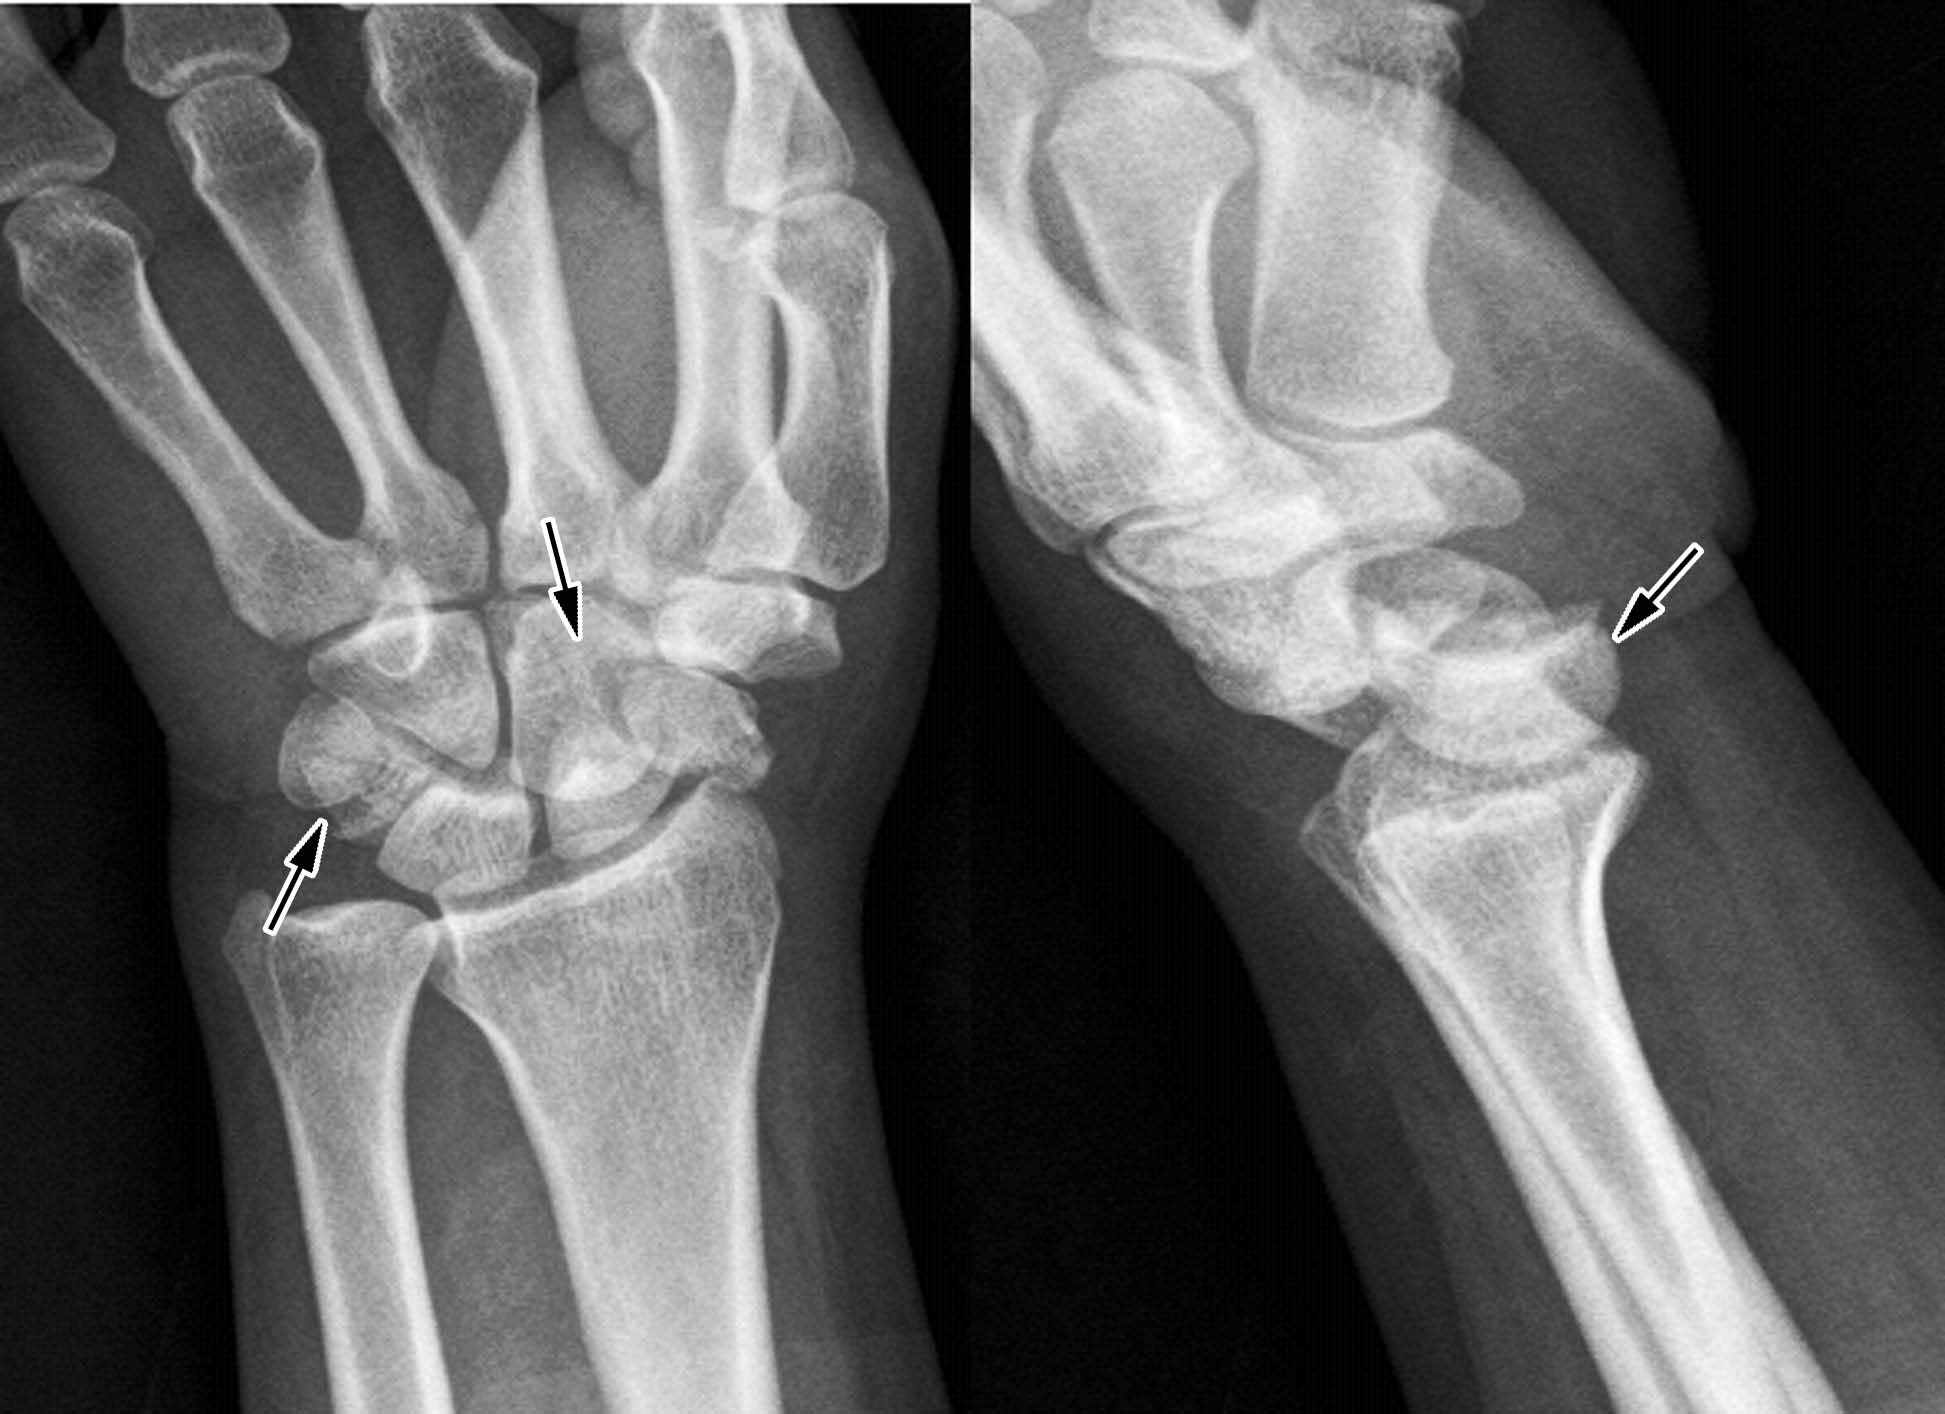
\includegraphics{./images/Image00040.jpg}
 \captionsetup{justification=centering}
 \caption{腕关节正侧位}
 \label{fig2-3-13}
  \end{figure} 

\textbf{【病史摘要】}
 女性,53岁。跌倒后左手掌撑地,左腕关节疼痛,关节肿胀,活动障碍。

\textbf{【X线表现】}
 正位片左手舟骨见透亮线影、断端分离,三角骨见裂隙影(箭头);侧位片见左手月骨向前移位、凹面向前(箭头)。

\textbf{【X线诊断】}  左腕月骨前脱位,伴手舟骨、三角骨骨折。

\textbf{【评  述】}
 腕骨脱位中最常见的是月骨前脱位,当摔倒且腕部处于极度背伸位时着地,月骨则被挤压于桡骨下端和头状骨之间,加之周围韧带及关节囊破裂,月骨脱离背侧韧带的束缚而向掌侧推出,并翻转凹面向前,X线正位片可显示头月关节间隙消失,侧位片表现为月骨脱出于掌侧。需与月骨周围脱位、经手舟骨月骨周围脱位鉴别。月骨周围脱位表现为月骨原位不动,与桡腕关节面保持正常位置,只有头骨和其他诸腕骨一起向背侧脱位;经手舟骨月骨周围脱位,实际上就是月骨周围脱位伴有手舟骨骨折,月骨与近侧手舟骨原位不动,与桡腕关节面保持正常位置,只有头骨和远侧手舟骨及其他诸腕骨一起向背侧脱位。

手舟骨位于腕关节的外侧部,分为腰、体、结节3个部分。由桡侧副韧带、桡头韧带、桡舟韧带和背侧韧带来维持它的稳定性。尤其与月骨间有坚强的舟月骨间韧带。整个手舟骨大部分为软骨所覆盖。其血供主要来自桡动脉的掌侧和背侧分支。桡动脉深支在手舟骨腰部背侧分2~4支细小动脉进入骨内。30%血运由掌侧支从手舟骨结节处进入手舟骨远端。内部血管走行是从外向内斜行,所以手舟骨脱位后必将由外经内走行的骨内血管损伤造成手舟骨缺血,影响骨的营养、再生和愈合。

腕关节前后位片(旋后位)上手舟骨变短,手舟骨结节呈环状,手舟骨与月骨间关节的间隙>2mm,即Terry-Thomas征阳性。

\subsection{肋骨不全骨折}

\begin{figure}[!htbp]
 \centering
 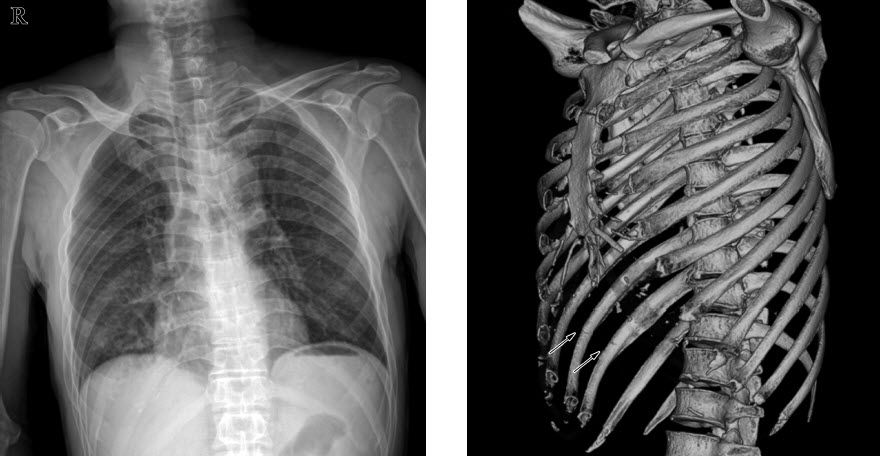
\includegraphics{./images/Image00041.jpg}
 \captionsetup{justification=centering}
 \caption{肋骨正位、右斜位}
 \label{fig2-3-14}
  \end{figure} 

\textbf{【病史摘要】}
 男性,52岁。车祸伤及右胸部,疼痛1小时,体检右前胸压痛(+)。

\textbf{【X线表现】}
 双侧胸廓对称。气管尚居中。右侧肋间隙较左侧略缩小。所见右侧肋骨未见明显移位骨折,第9,10腋肋皮质欠光整。双肺内未见明显异常。心脏大小属正常。右侧膈面外1/3略上移。右侧肋膈角略钝。左侧肋膈角锐利。

\textbf{【X线诊断】}
 右侧第9,10肋骨不全骨折可能,伴少量右侧胸腔积液可能,建议肋骨CT三维重建检查。

\textbf{【评  述】}
 肋骨骨折在胸部损伤中发生率为40%~60%。常发生于中、老年人,很少见于儿童。这与骨质脆性增加有关。直接或间接暴力均可引起骨折。直接暴力骨折多发生在肋骨直接受打击部位,尖锐的骨折端向内移位,可刺破肋间血管、胸膜、肺组织或上腹部脏器,产生血胸、气胸或血气胸、皮下气肿、咯血等。间接暴力(胸部前后受挤压)骨折发生在暴力作用点以外的部位,多见于肋骨角或肋骨体部,骨折端向外移位,可损伤胸壁软组织,产生胸壁血肿。肋骨骨折以第4~7肋最常见,因其较长且固定,容易折断。第1~3肋骨较短,且有锁骨、肩胛骨和肌肉的保护,很少发生骨折。第8~10肋骨虽较长,但不与胸骨直接连接,而连接于肋弓上,有弹性缓冲,较不易折断。第11及12肋骨为浮肋,前端游离不固定,活动度较大,骨折更为少见。但外来强大暴力亦可引起这些肋骨骨折。肋骨骨折可发生在单根或多根肋骨,同一肋骨可在一处或多处折断,甚至多根多处骨折(多于3根肋骨)而产生“浮动胸壁”,出现反常呼吸运动。较大面积的“浮动胸壁”,严重影响呼吸回流功能,可出现气短、发绀或呼吸困难。如并发肺裂伤,可有咯血、气胸、血胸或皮下气肿。年老、体弱患者,肋骨骨折同时可并发肺炎、肺不张。肋骨骨折的X线检查,最容易漏诊,其原因有:①无移位性骨折,因肋骨结构单薄缺乏对比,无移位的骨折线比较细微,又多与肺纹理重叠,故容易漏诊。特别是当骨折处咬合较紧密时,早期X线检查骨折线可不显示或不明显显示,而较容易引起漏诊;但当患者受伤一段时间后,由于活动或者牵拉,骨折处由咬合紧密而变为分离,此时X线检查可明显显示骨折线而确立诊断;因此,当早期X线检查未显示骨折线而临床症状明显时,应提醒患者及时复查及时发现,以免漏诊。②肋骨腋段骨折,因该段肋骨呈半圆形,且前后重叠较多,在正位片上因相互重叠而影响了骨折线显示。③照片伪影的影响,有些患者因疼痛等原因屏气不好,或体位不正,造成了细微骨折线显示不清。X线诊断肋骨骨折时,如骨折线显示不清,有时需结合其他继发征象观察,如胸腔积血、皮下纵隔气肿、气胸、胸壁软组织肿胀及胸膜影增厚等。CT三维肋骨重建可多角度观察肋骨形态,显示轻微骨折线(箭头)。当X线检查不能明确时,可建议采用CT三维重建检查。

\subsection{肋骨骨折}

\begin{figure}[!htbp]
 \centering
 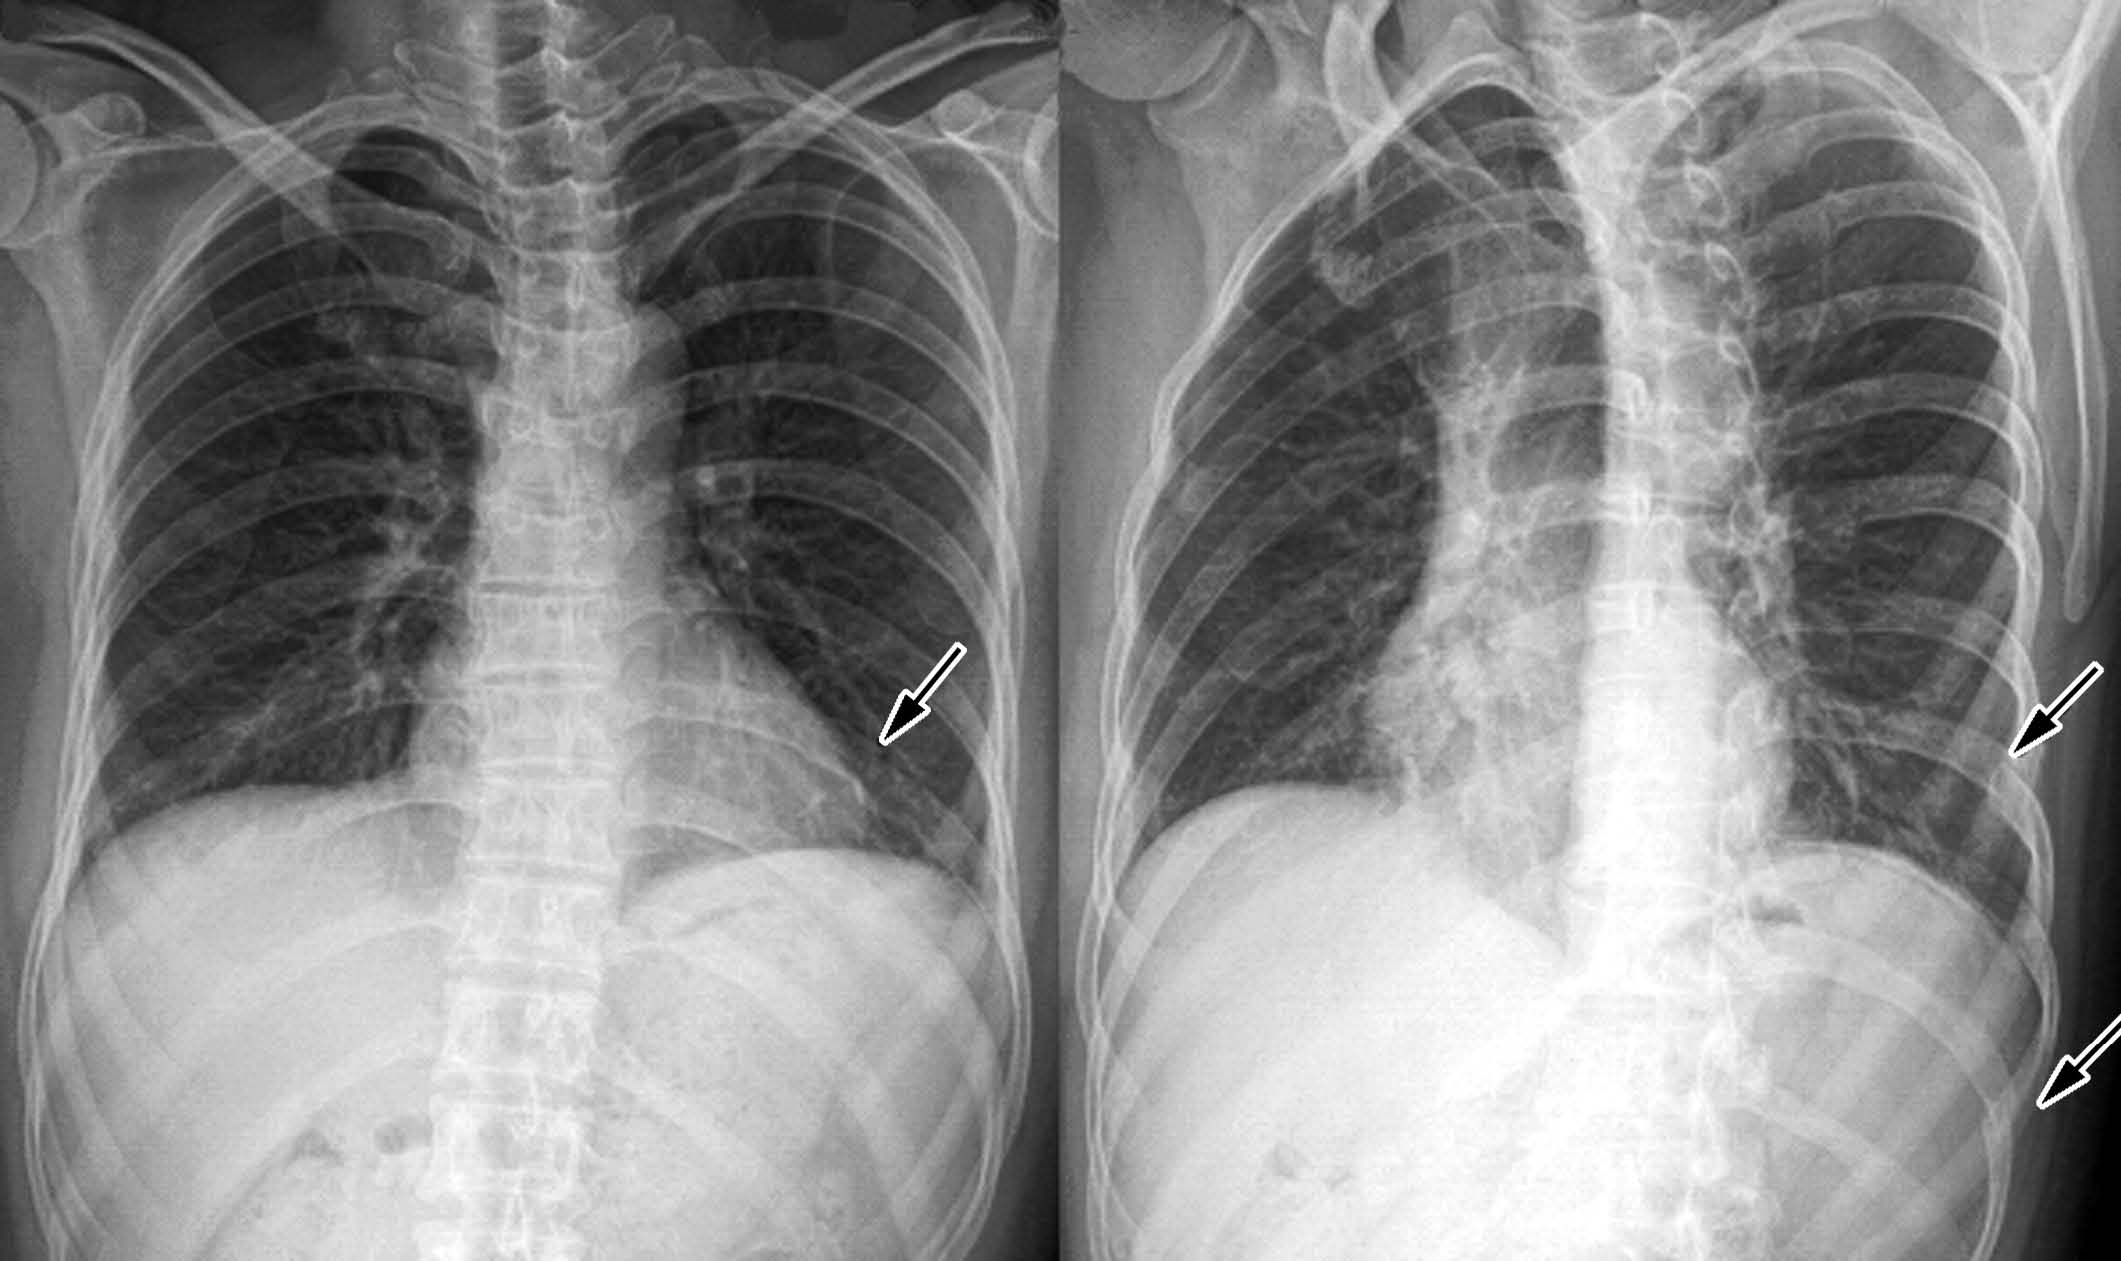
\includegraphics{./images/Image00042.jpg}
 \captionsetup{justification=centering}
 \caption{肋骨正位、左斜位}
 \label{fig2-3-15}
  \end{figure} 

\textbf{【病史摘要】}  男性,46岁。左胸部撞伤,胸部疼痛。

\textbf{【X线表现】}
 正位片示左侧第9肋见骨折线(箭头),斜位片示左侧第9、11肋骨见骨折线(箭头)。

\textbf{【X线诊断】}  左侧第9、11肋骨新鲜骨折。

\textbf{【评  述】}
 怀疑肋骨骨折时一定要同时摄正、斜位片。如果受伤当时断端移位不明显,拍X线片可能不显示骨折线,1周或半个月后,当断端出现移位或骨痂形成时则易显示。故胸部受伤后,若平片未发现骨折,而临床又高度怀疑时,应行螺旋CT扫描或随诊摄片观察。需与陈旧性肋骨骨折、病理性肋骨骨折及自发性肋骨骨折鉴别。陈旧性肋骨骨折一般骨折线显示不清,断端可见骨痂形成;病理性肋骨骨折指肋骨由于先前已经存在的病变(如原发肿瘤、转移瘤、骨纤维异常增殖症等)使其强度下降,很小的外力或没有外力作用下亦可发生骨折;自发性肋骨骨折是由于剧烈的咳嗽或喷嚏等引起胸部肌肉强烈收缩而发生。

可疑多发伤的患者急诊需要强制性摄三个部位的X线平片:①颈椎的侧位片;②胸片(排除纵隔血肿、气胸、血胸、肋骨骨折和肺挫伤);③前后位骨盆片。

若X线平片和CT常规扫描均不能发现隐匿性肋骨骨折时,肋骨的CT三维重建尤其是表面重建图像对骨折的诊断有一定帮助。

\subsection{股骨颈骨折}

\begin{figure}[!htbp]
 \centering
 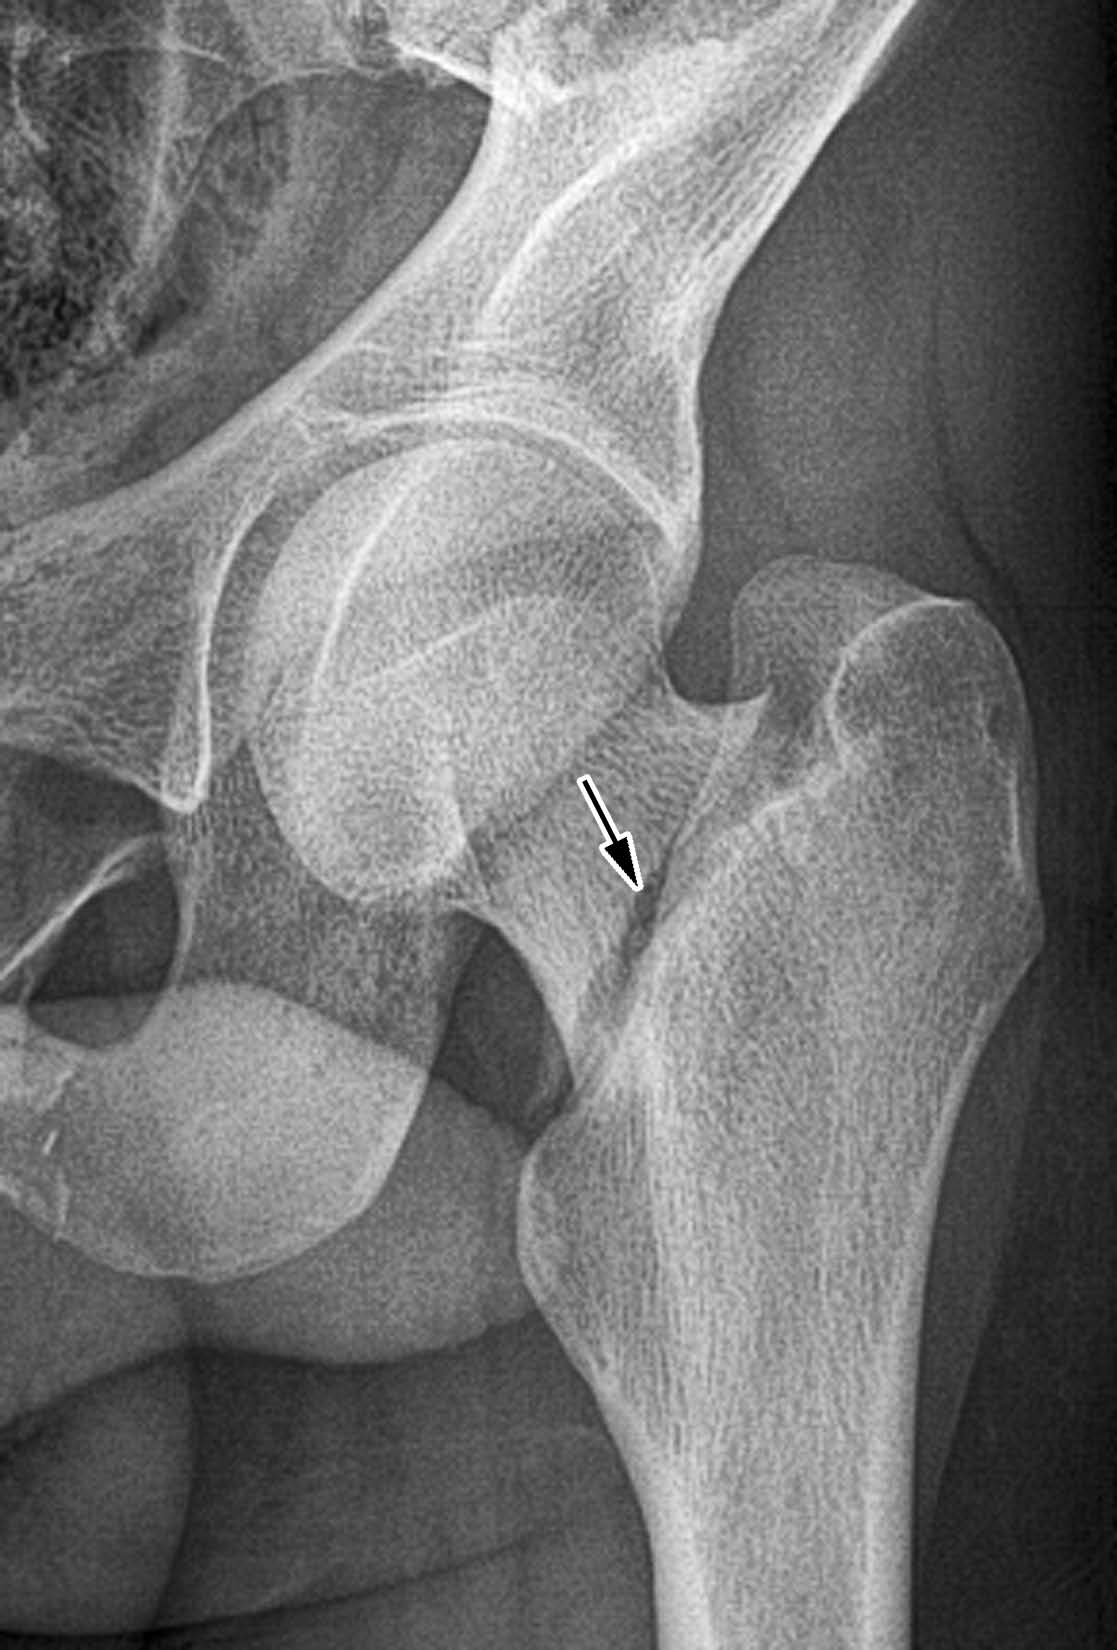
\includegraphics{./images/Image00043.jpg}
 \captionsetup{justification=centering}
 \caption{左髋关节正位}
 \label{fig2-3-16}
  \end{figure} 

\textbf{【病史摘要】}
 女性,68岁。摔倒后左臀部着地,左髋部肿胀,活动障碍,患肢轻度缩短、外旋畸形。

\textbf{【X线表现】}
 左股骨颈基底部见透亮线影,断端对位、对线良好(箭头)。

\textbf{【X线诊断】}  左股骨颈基底部骨折。

\textbf{【评  述】}
 股骨颈骨折是髋关节中最常见的一种创伤,老年人骨质疏松、轻微外伤即可引起骨折,青壮年多为暴力所致。按发生部位,股骨颈骨折可分为头下部、中央部及基底部三型:头下部和中央部属关节囊内骨折,骨折近侧断端因与关节囊分离而血运不足,易发生股骨头缺血性坏死,骨折愈合困难;基底部骨折属关节囊外骨折,血运障碍少,易愈合。隐匿性股骨颈骨折在X线与CT上容易漏诊,需仔细观察股骨颈张力骨小梁、应力骨小梁和骨皮质是否连续,诊断困难时应行MR检查,且MR能早期发现股骨头缺血性坏死。X线对鉴别外展、嵌顿、稳定型与内收、非嵌顿、不稳定型股骨颈骨折有帮助。前者少见,多数为头下部骨折,在有嵌顿的骨折中骨折线显示不清,而表现嵌插后骨小梁压缩的致密带,外展型的骨折线与股骨干纵轴的垂线的交角(Linton角)一般小于30°,骨折线剪力小,愈合率高;后者较多见,多数为中央部骨折,Linton角一般大于50°,骨折线剪力大、易移位,愈合率低,在不适当的治疗下,外展、嵌顿骨折可以转变为有移位的内收骨折。

\subsection{股骨转子间骨折}

\begin{figure}[!htbp]
 \centering
 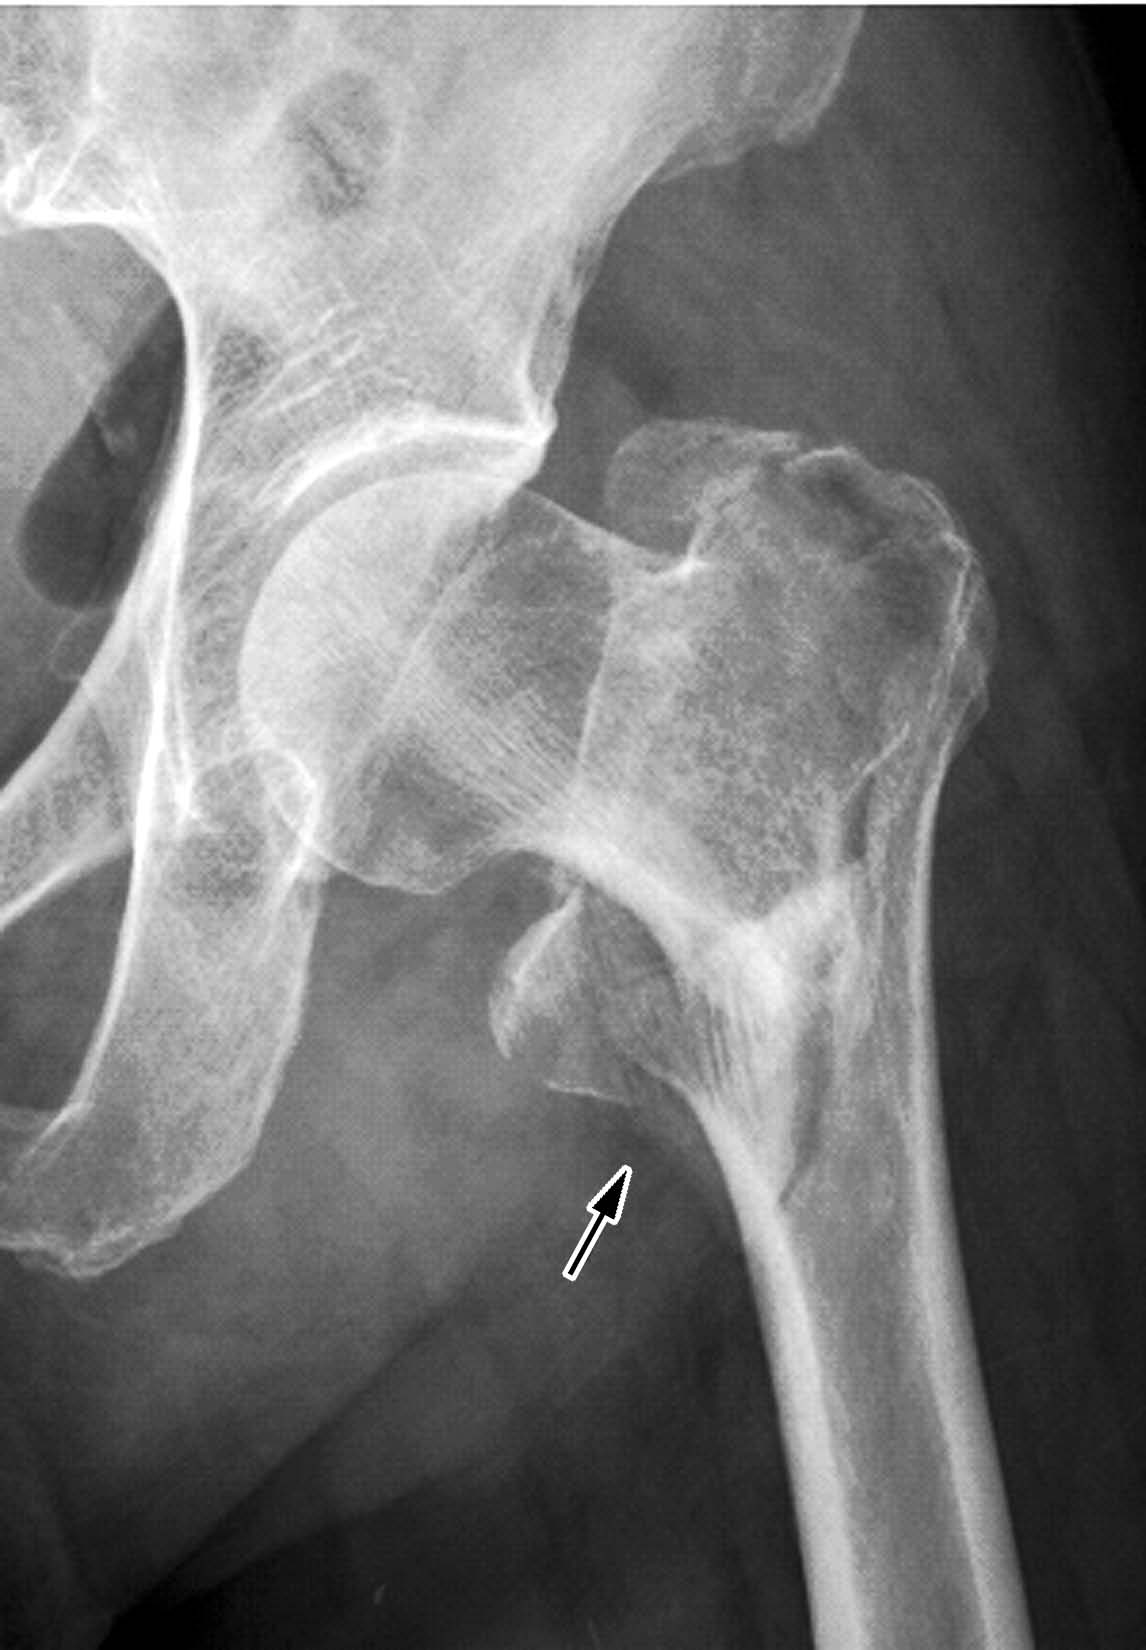
\includegraphics{./images/Image00044.jpg}
 \captionsetup{justification=centering}
 \caption{左髋关节正位}
 \label{fig2-3-17}
  \end{figure} 

\textbf{【病史摘要】}
 女性,67岁。撞倒后左臀部着地,左髋部肿胀,活动障碍。

\textbf{【X线表现】}
 左股骨大小转子见透亮线影,远端有轻度外旋(箭头)。

\textbf{【X线诊断】}  左股骨转子间骨折。

\textbf{【评  述】}
 股骨转子间骨折多为老年人,其创伤机制包括直接暴力与间接暴力,直接暴力即直接作用于大小转子间,间接暴力指大小转子受到内翻及向前成角的复合应力。骨折线的形态多自大转子斜行向下至小转子,骨折常为粉碎型。转子间骨折较易愈合,但易产生髋内翻畸形。稳定型与不稳定型股骨转子骨折鉴别诊断:前者的骨折线自大转子斜向内下方到小转子,可合并小转子纵行骨折,此型多见;后者的骨折线则自小转子向外下达大转子下方,上骨折端受臀肌牵拉外展,向外错位,此型少见。

\subsection{髋关节前脱位}

\begin{figure}[!htbp]
 \centering
 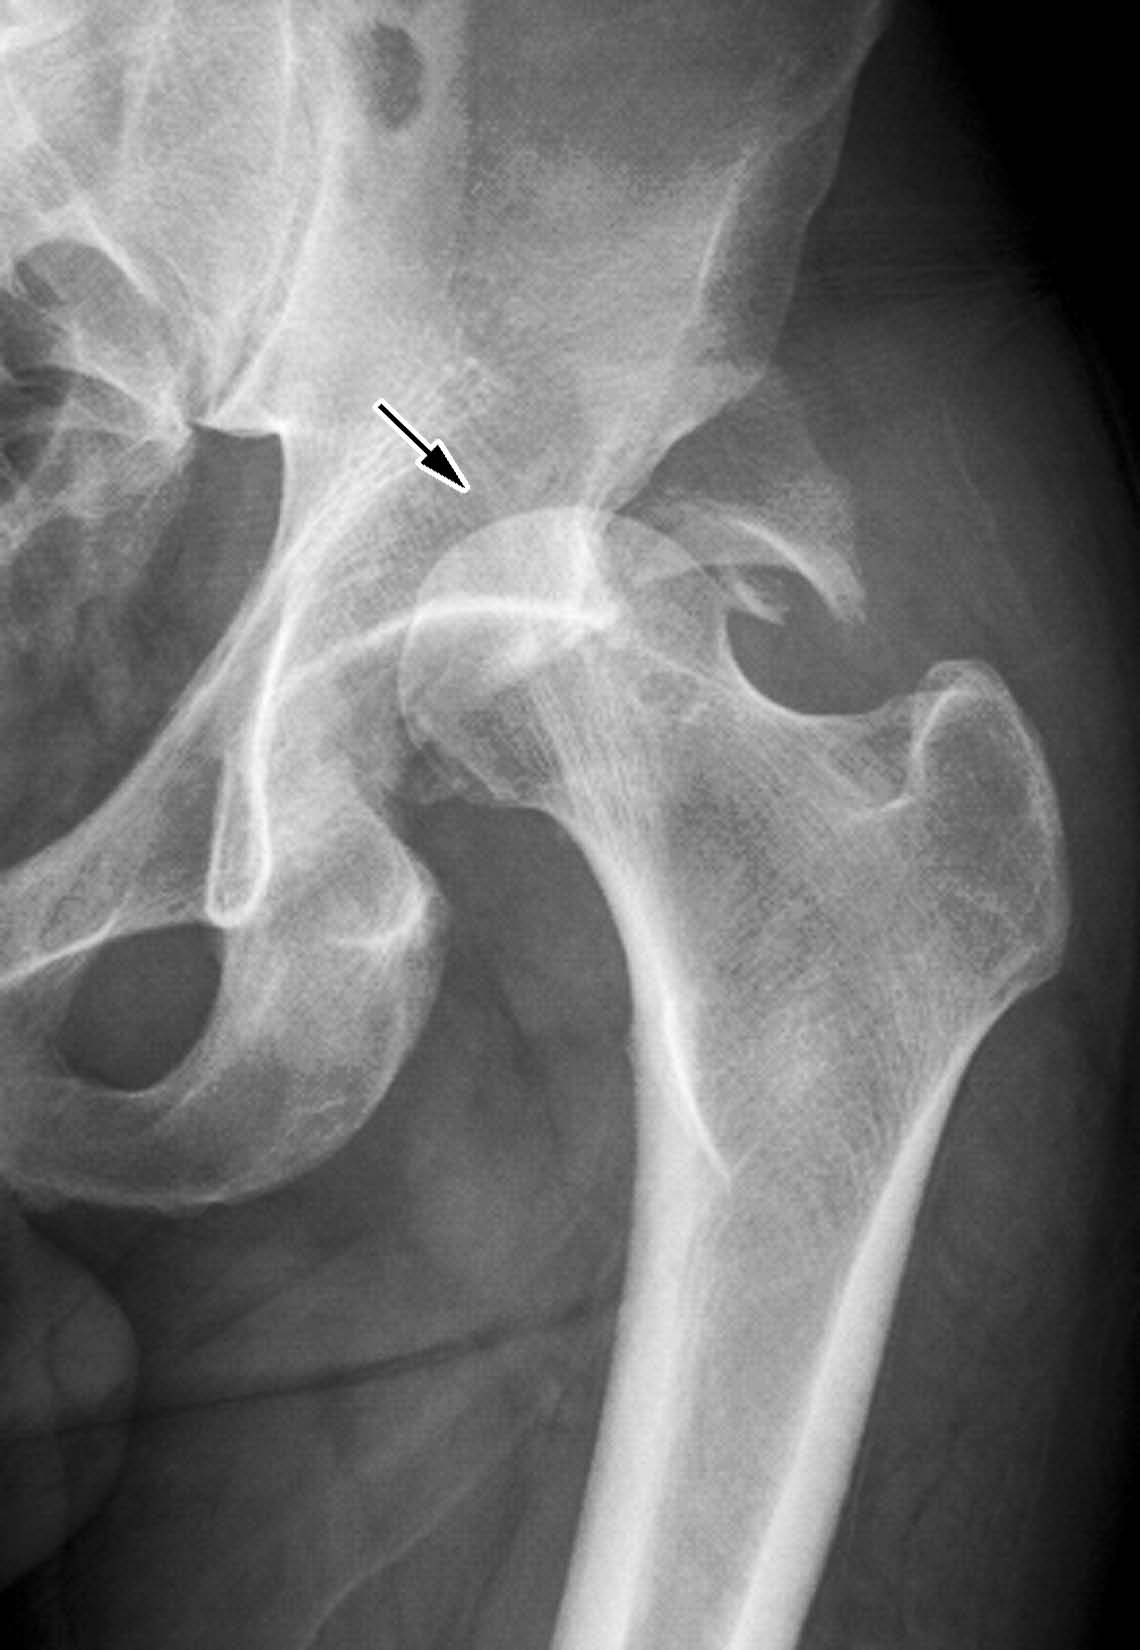
\includegraphics{./images/Image00045.jpg}
 \captionsetup{justification=centering}
 \caption{左髋关节正位}
 \label{fig2-3-18}
  \end{figure} 

\textbf{【病史摘要】}
 男性,49岁。被撞倒后左股骨外展畸形,左髋关节活动障碍。

\textbf{【X线表现】}  左股骨头向髋臼前、上移位(箭头)。

\textbf{【X线诊断】}  左髋关节前脱位。

\textbf{【评  述】}
 髋关节结构稳固,必须有强大的外力才能引起脱位,因而是一种严重损伤,在脱位时常伴有的骨折及周围软组织损伤亦较严重。髋关节脱位在X线上均表现为髋臼与股骨头失去正常对应关系,一般诊断不难,CT容易发现X线平片遗漏的骨折碎片。

三种类型的髋关节脱位鉴别:①前脱位,大腿急骤外展、外力从臀部向前冲击时所致。正位X线见股骨干外展水平位,股骨头脱出于髋臼下方,与闭孔同高,并与坐骨结节重叠。②中心脱位,当强暴力作用大转子或沿股骨干向髋臼冲击时,可造成髋臼底骨折,随后股骨头向盆腔内突出所致,X线表现为髋臼呈粉碎性骨折,髋臼窝分为上、下两半,部分髋臼底被股骨头冲击向骨盆内转移,股骨头也随之向盆腔内突出,也可发生骶髂关节和耻骨联合韧带的撕裂与分离,甚至耻骨骨折。③后脱位,多见,当大腿屈曲过度猛烈内收内旋,或大腿屈曲内收外力从膝沿股骨干向髋传导时所致,患肢屈曲、内收、内旋及缩短畸形,常伴有髋臼后上缘骨折。

\subsection{髌骨骨折}

\begin{figure}[!htbp]
 \centering
 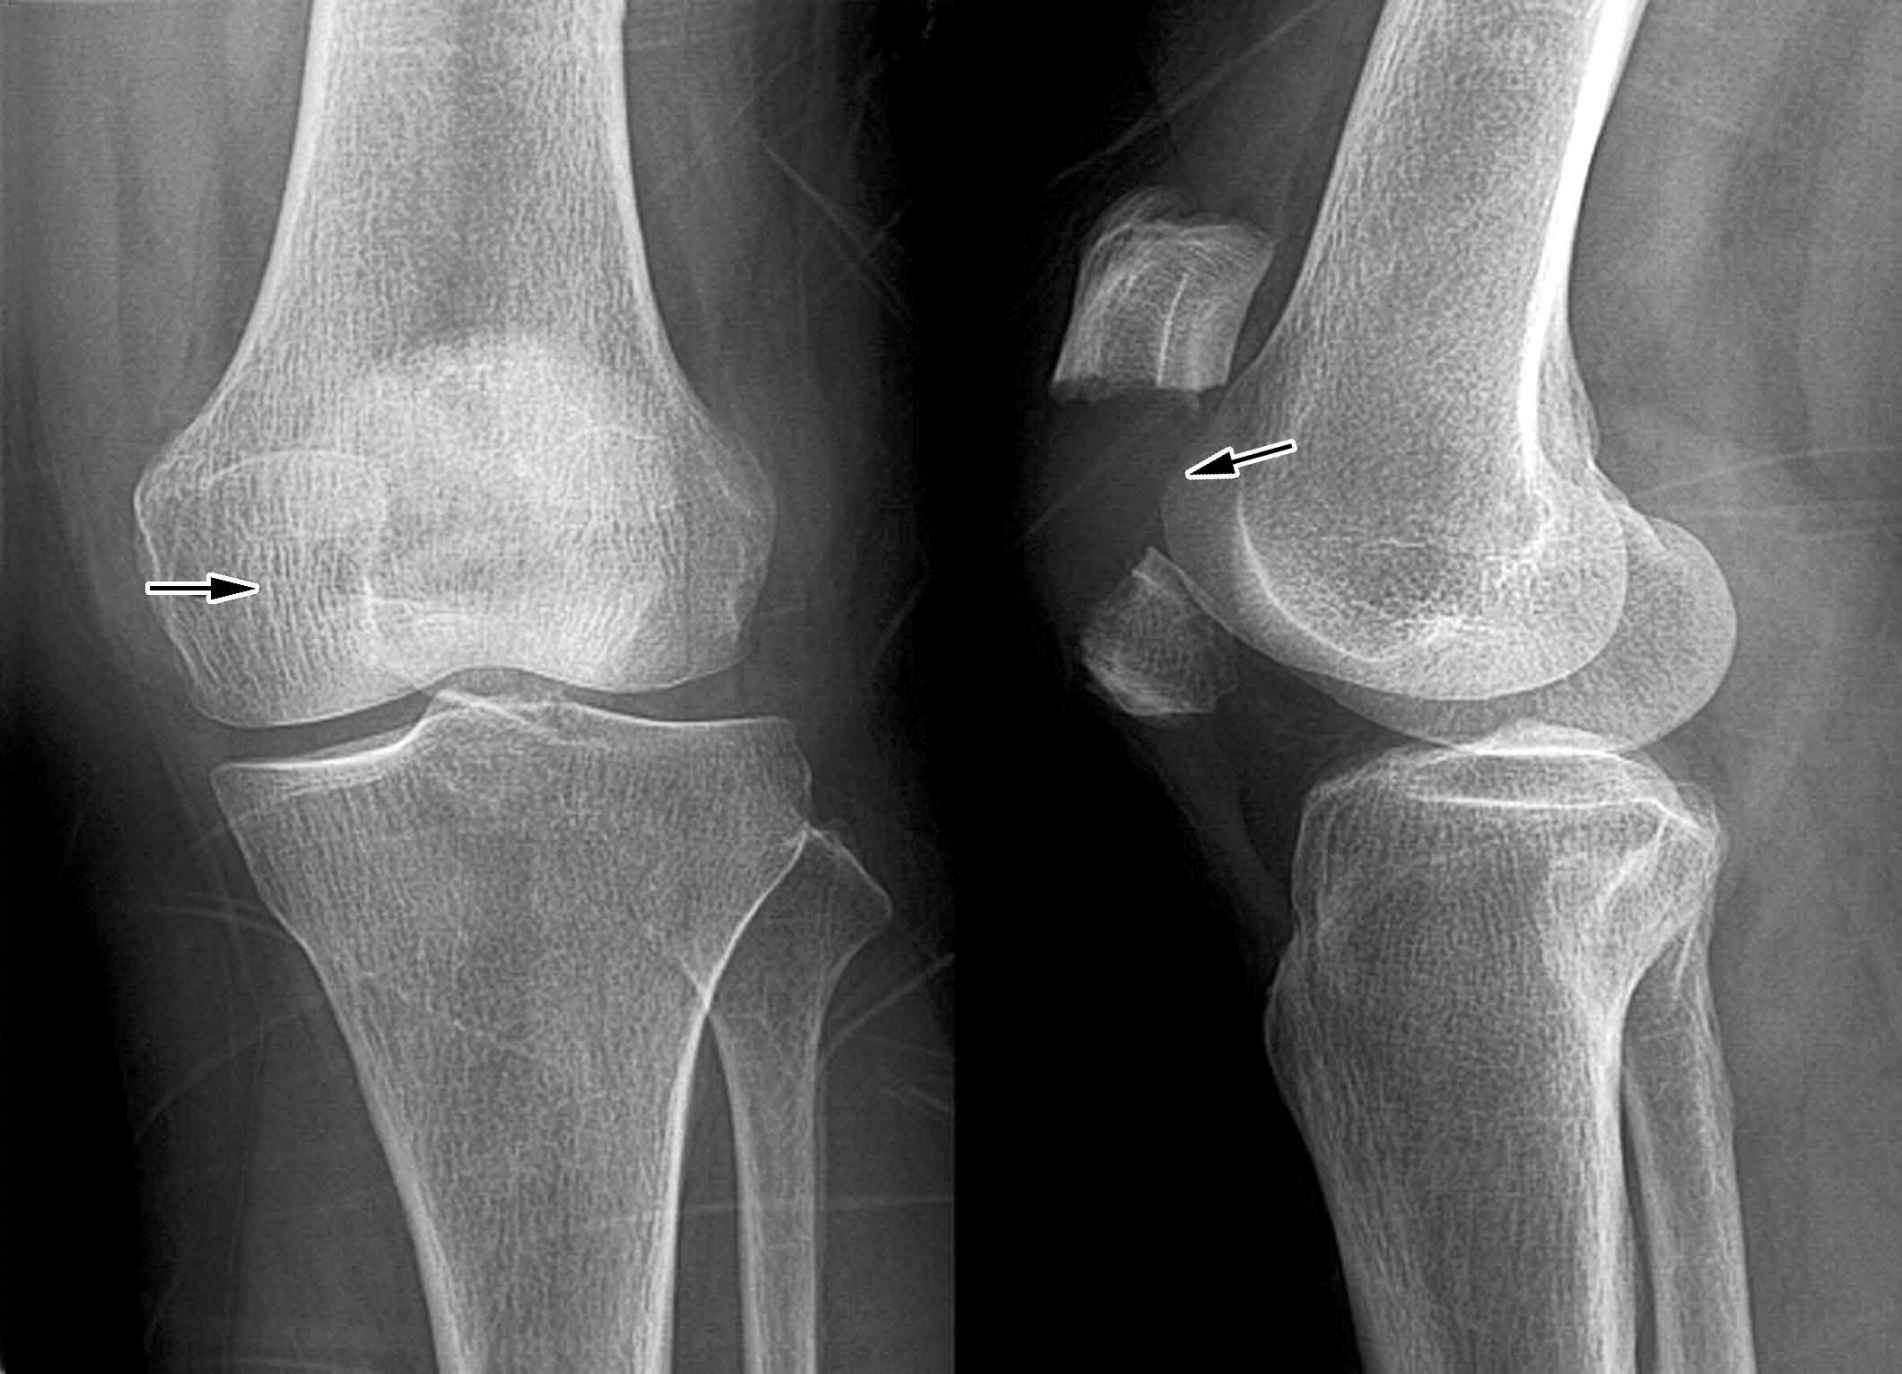
\includegraphics{./images/Image00046.jpg}
 \captionsetup{justification=centering}
 \caption{膝关节正侧位}
 \label{fig2-3-19}
  \end{figure} 

\textbf{【病史摘要】}
 男性,46岁。摔倒后左膝部着地,左膝关节疼痛,活动受限,关节肿胀。

\textbf{【X线表现】}  左侧髌骨断裂,断端分离较远(箭头)。

\textbf{【X线诊断】}  左侧髌骨骨折。

\textbf{【评  述】}
 髌骨骨折较常见,多为30~50岁。男性多于女性,间接暴力所造成的骨折多为横行骨折。直接暴力所致骨折多为星状粉碎性骨折,骨片可无移位。若正侧位骨折线显示不清,而临床症状明显时,应加摄髌骨轴位片,以免漏诊。

鉴别诊断:①发生在髌骨边缘的骨折,X线片上髌骨可以光滑、完整,与正常无异。②髌骨软骨袖套状骨折,X线表现正常髌骨形态发生变化,在髌骨上方或下方有发丝样、蛋壳样或袖套状的较淡影像,必要时可行MR检查。③髌骨是人体中最大的籽骨,在出生时完全为透明软骨构成,2~5岁时出现骨化中心,17~18岁时骨化完成,髌骨一般只有一个骨化中心。但是个别少年可出现一个或多发副骨化中心,常位于髌骨外上角。如果副骨化中心在髌骨发育成熟后不与主骨融合,即二分或多分髌骨。二分髌骨极易误诊为髌骨骨折,其主要原因:①询问病史、查体不详细;②阅片不仔细或X线片质量不高,仅凭单一体位X线片作出诊断;③医师对二分髌骨缺乏了解和认识;④忽略了患者体征与X线片的统一。

\subsection{胫骨平台内侧髁骨折}

\begin{figure}[!htbp]
 \centering
 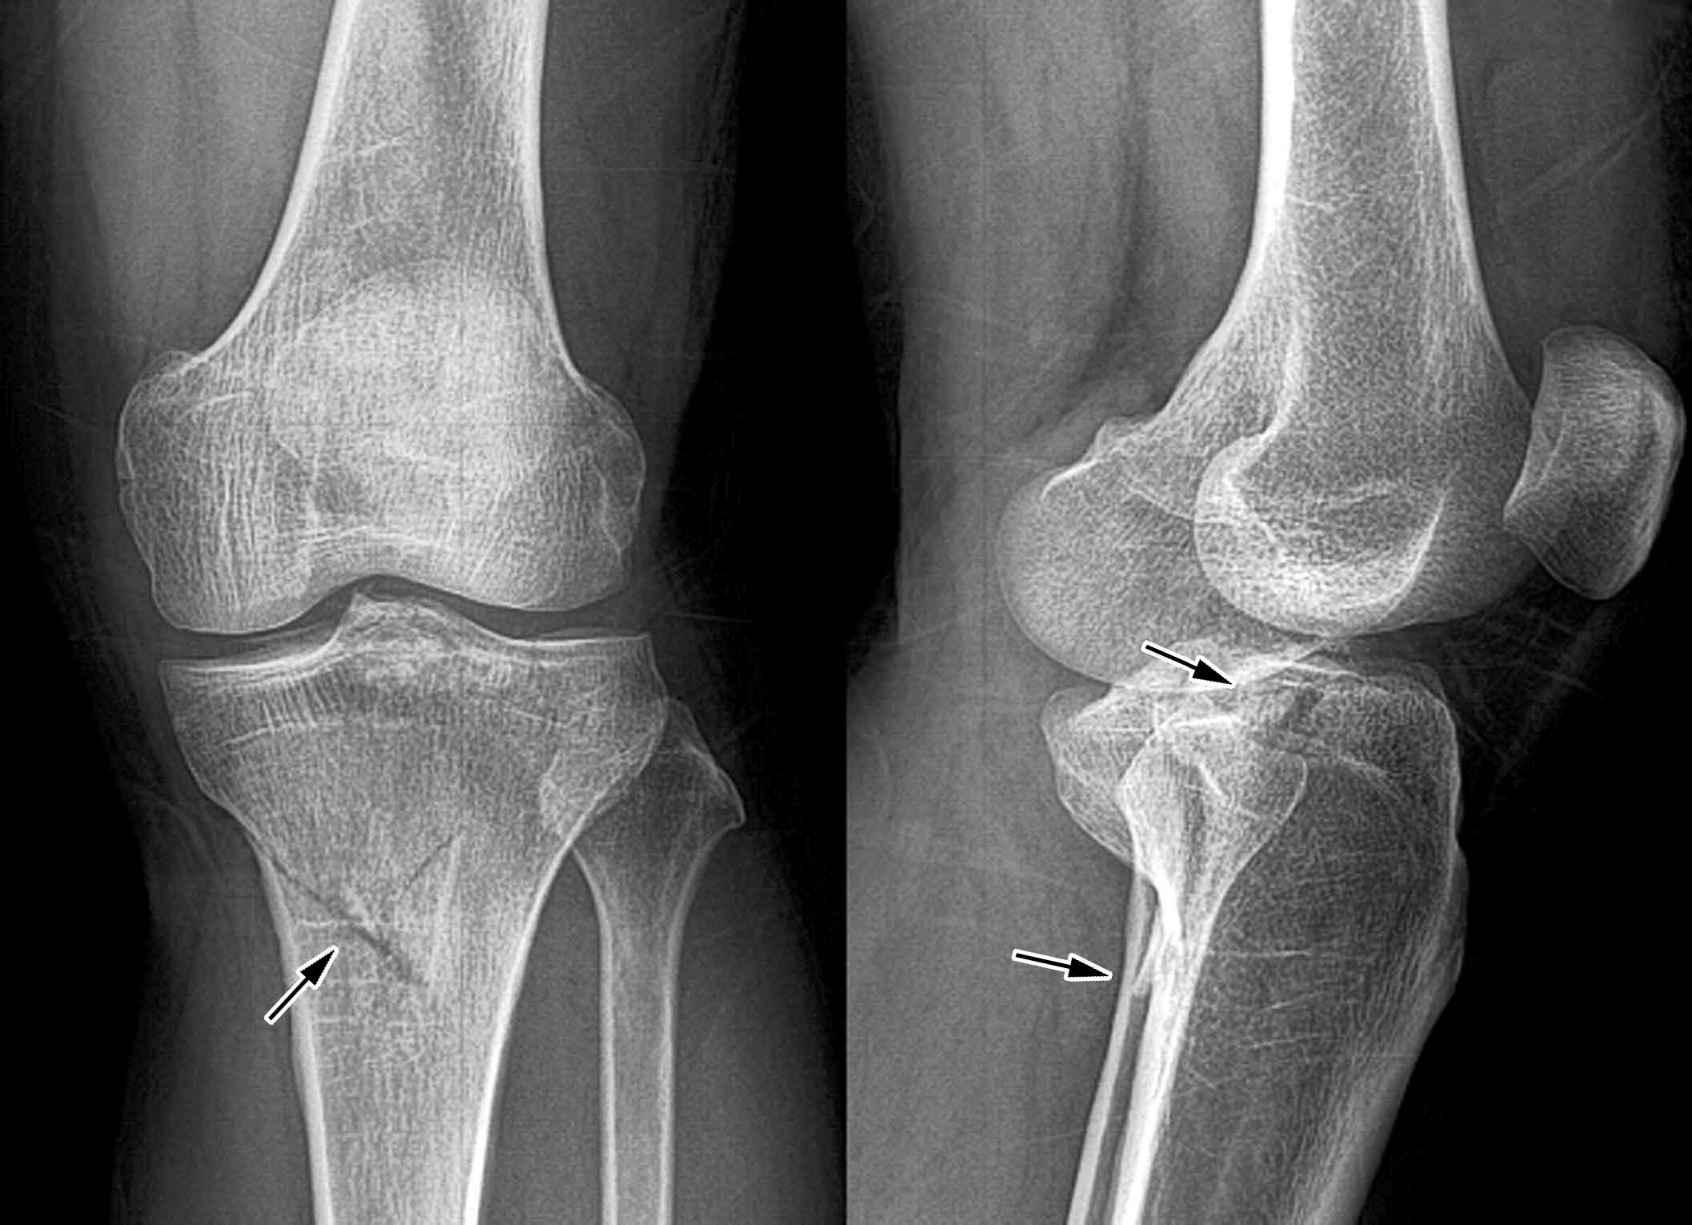
\includegraphics{./images/Image00047.jpg}
 \captionsetup{justification=centering}
 \caption{膝关节正侧位}
 \label{fig2-3-20}
  \end{figure} 

\textbf{【病史摘要】}
 女性,66岁。从楼梯摔下,左膝部着地,左胫骨上段疼痛,左膝关节肿胀。

\textbf{【X线表现】}
 左胫骨上端内侧髁见多发斜行及纵行透亮线影(箭头)。

\textbf{【X线诊断】}  左胫骨平台内侧髁骨折。

\textbf{【评  述】}
 胫骨髁或平台骨折多见于青壮年,骨折多为传达暴力所致,如从高处坠下、足底着地。胫骨内、外髁受相等压力时,可同时发生骨折。压力不等时,压力大的一侧发生骨折。膝关节过度外翻或内翻,亦可造成单髁骨折,并合并内、外侧副韧带的撕裂。胫骨髁骨折多为压缩、劈裂及粉碎性骨折,外髁骨折可合并腓骨颈骨折。胫骨髁骨折多累及关节面,关节腔内常积血,半月板和十字韧带可发生损伤。胫骨平台骨折可分为六种类型(Schatzker分型):Ⅰ型,外侧平台的单纯楔形骨折或劈裂骨折;Ⅱ型,外侧平台的劈裂压缩性骨折;Ⅲ型,外侧平台单纯压缩性骨折;Ⅳ型,内侧平台骨折,其可以是劈裂性或劈裂压缩性;Ⅴ型,包括内侧平台与外侧平台劈裂的双髁骨折;Ⅵ型,同时有关节面骨折和干骺端骨折,胫骨髁部与骨干分离,即所谓的骨干-干骺端分离,常伴有相当严重的关节破坏、粉碎、压缩及髁移位。

\subsection{Segond骨折}

\begin{figure}[!htbp]
 \centering
 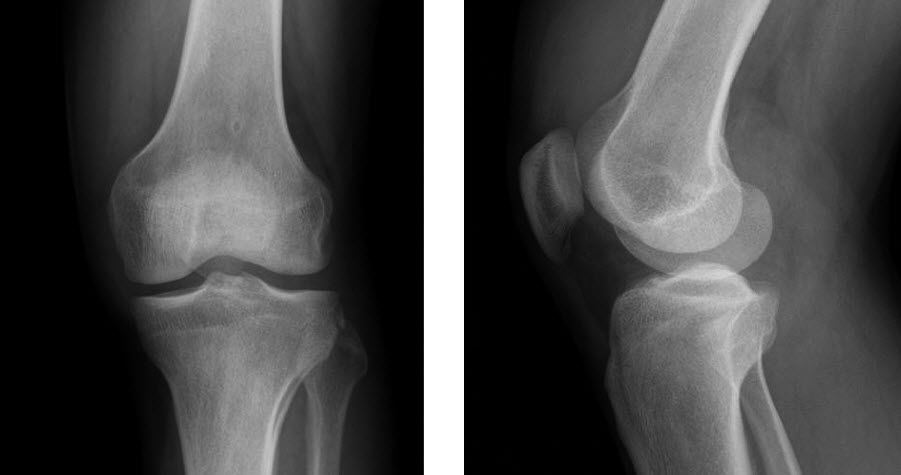
\includegraphics{./images/Image00048.jpg}
 \captionsetup{justification=centering}
 \caption{左膝关节正侧位}
 \label{fig2-3-21}
  \end{figure} 

\textbf{【病史摘要】}
 男性,38岁。下蹲搬重物时扭伤左膝关节,左膝关节外侧缘疼痛,关节肿胀。

\textbf{【X线表现】}
 左膝关节正位片示左侧胫骨平台外侧缘局限性撕脱性碎骨片,膝关节肿胀,关节间隙变宽,侧位片示股骨外侧沟向内凹陷大于2mm,前后缘脂肪垫消失。

\textbf{【X线诊断】}  左膝关节胫骨外侧缘Segond骨折。

\textbf{【评  述】}
 Segond骨折又称为胫骨平台外缘撕脱性骨折,该病由Paul
Segond于1879年首次报道,并以其名命名。发病机制为膝关节处于半屈曲位10°~90°时存在一个内旋应力致外侧副韧带前斜束止点的撕脱性骨折。Segond骨折常伴有前交叉韧带的断裂,由此可以作为诊断前交叉韧带断裂的线索。临床上该病表现为关节肿胀,很容易漏诊,前抽屉试验和Lachman实验不能确定交叉韧带是否损伤,即使早期MRI检查,有时也会因关节腔积液过多导致诊断困难,而X线检查简单易行,若表现为胫骨平台外侧缘小片撕脱性骨块,股骨外侧沟向内凹陷大于2mm,则高度提示前交叉韧带损伤可能,早期采取制动措施避免进一步损伤。当患者关节积液减少时再行MRI检查明确诊断。若单纯撕脱性骨折,仅需石膏固定即可,若损伤前交叉韧带,则需手术治疗。

\subsection{前交叉韧带损伤}

\begin{figure}[!htbp]
 \centering
 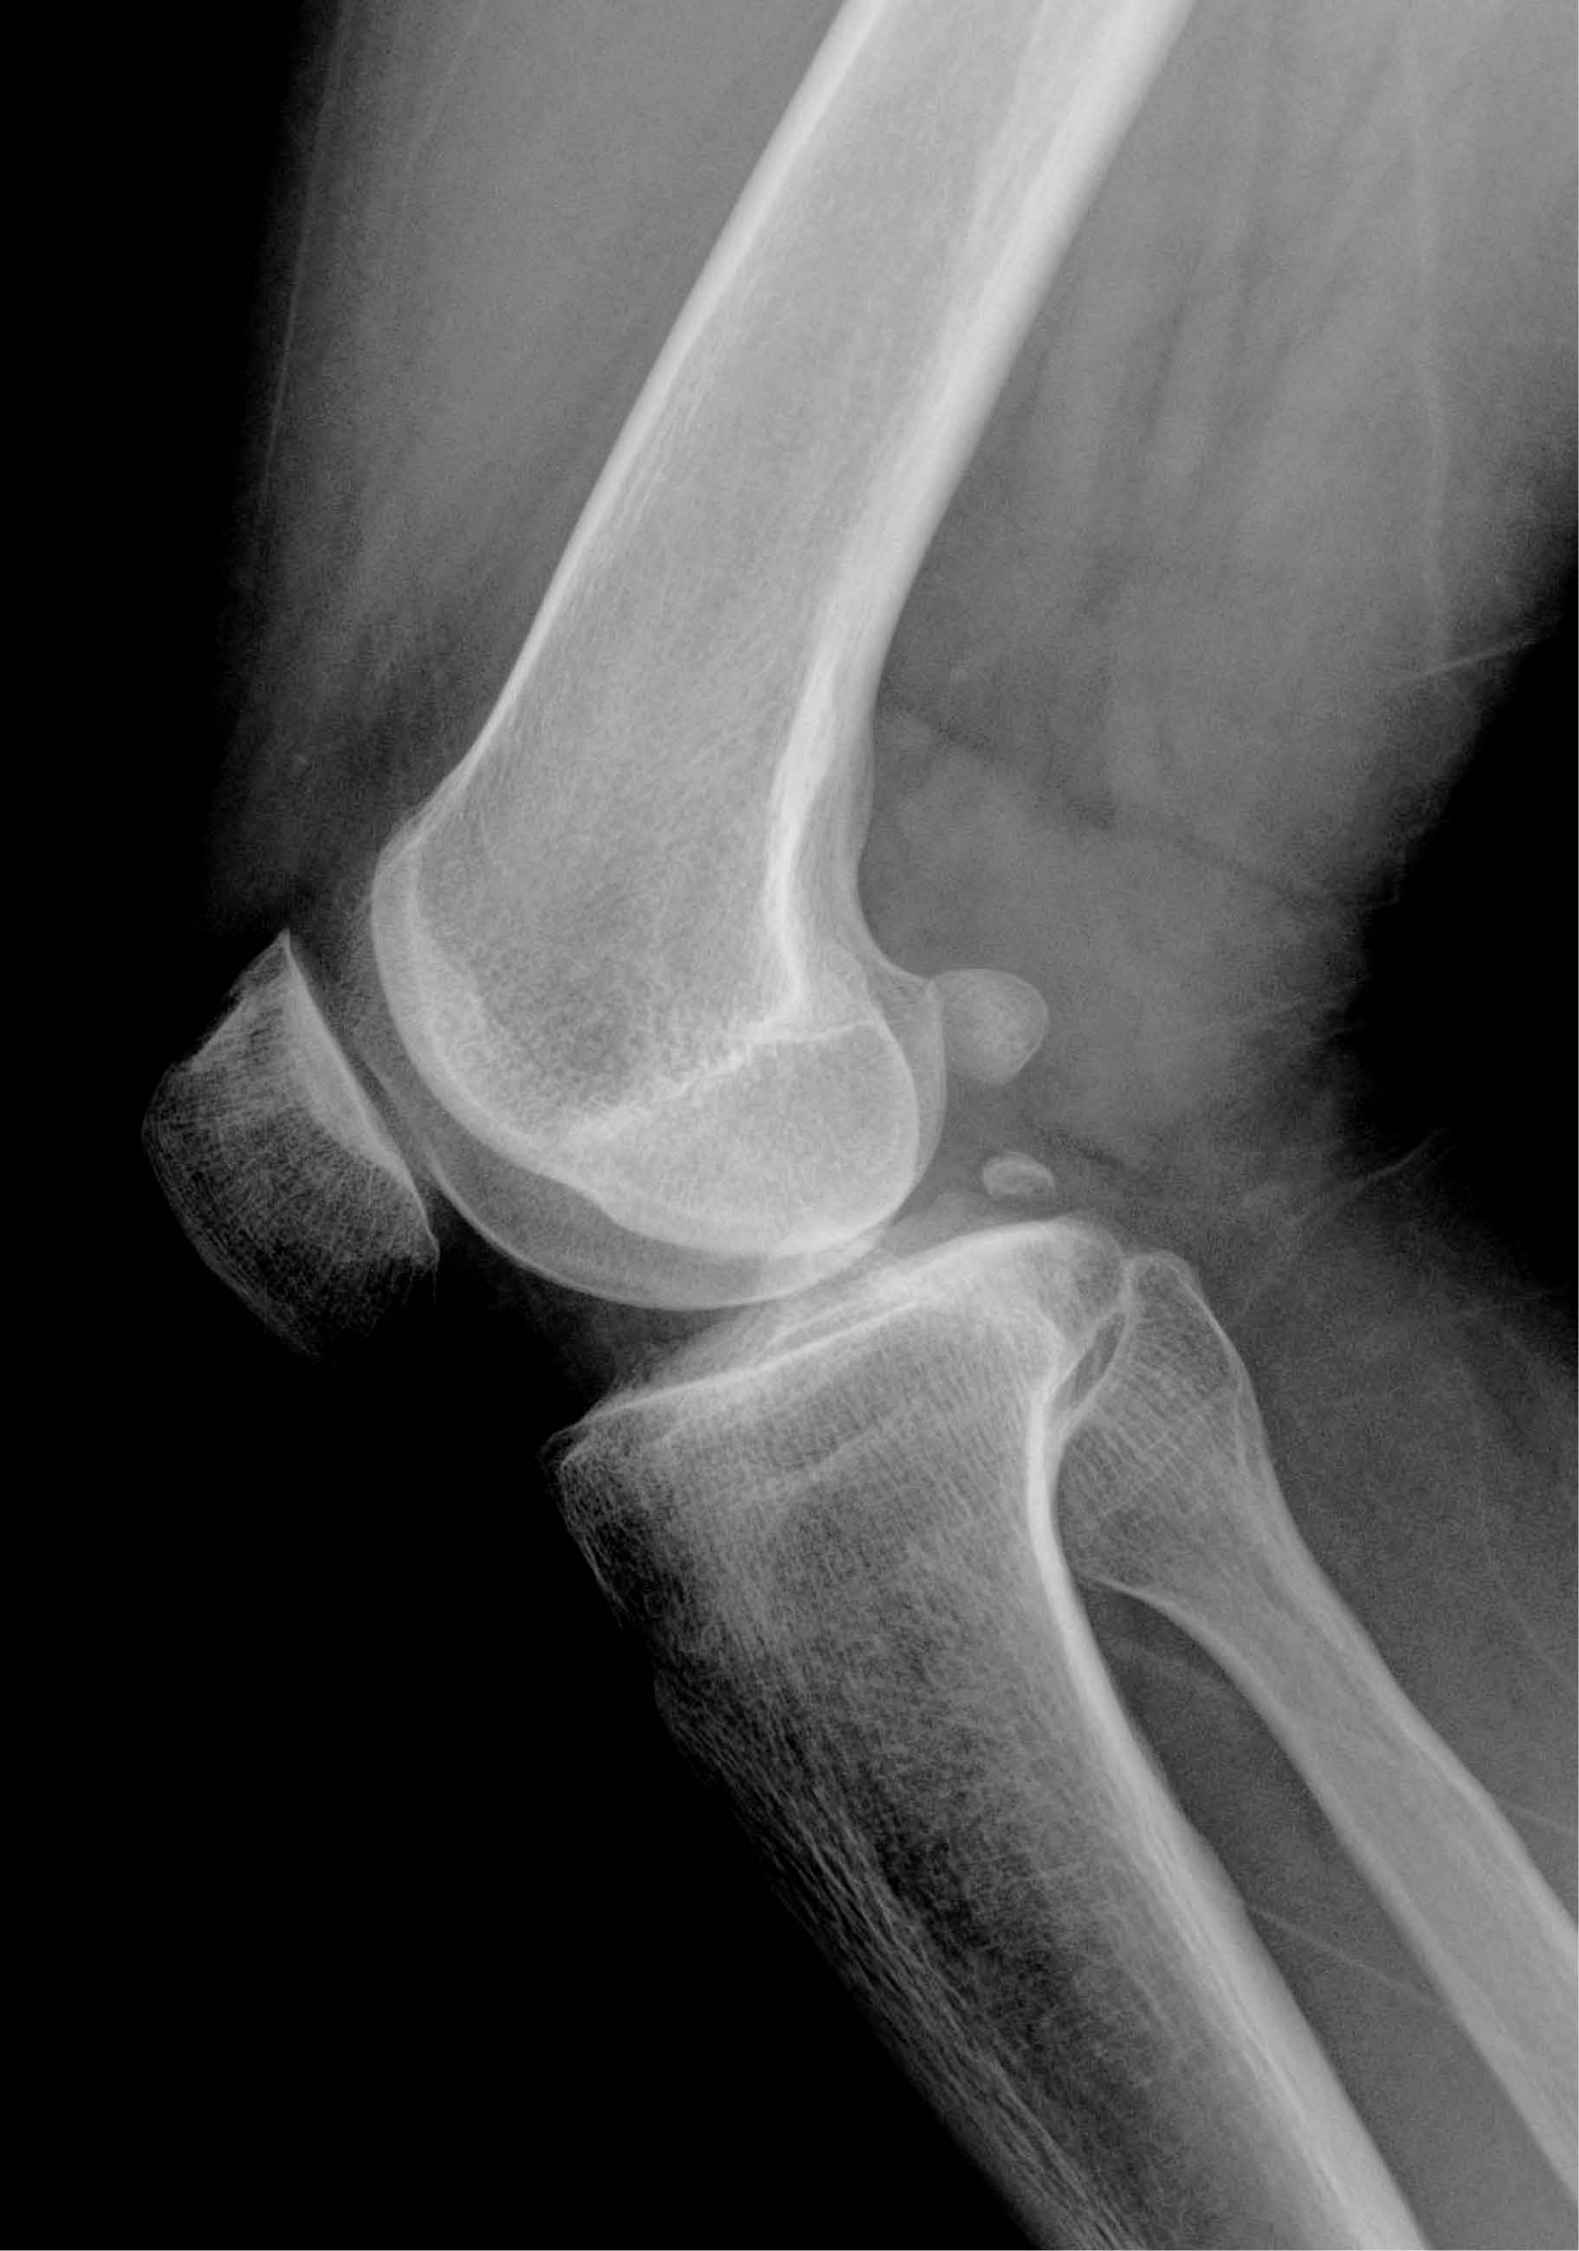
\includegraphics{./images/Image00049.jpg}
 \captionsetup{justification=centering}
 \caption{右膝关节侧位}
 \label{fig2-3-22}
  \end{figure} 

\textbf{【病史摘要】}
 男性,41岁。汽车侧方直接撞伤左膝关节,左膝肿胀疼痛。

\textbf{【X线表现】}
 左膝关节侧位片示骨皮质光整,未见明显骨折,股骨外侧沟局限性凹陷;膝关节后腘窝内见类圆形籽骨影,境界清楚。

\textbf{【X线诊断】}
 左膝关节股骨外侧局限性凹陷,考虑为前交叉韧带损伤所致。

\textbf{【评  述】}
 前交叉韧带止点撕脱骨折属于关节内骨折,好发于运动员,尤其是橄榄球和滑雪运动员。多为运动伤、交通事故伤,其损伤机制为膝关节外伤暴力后,前交叉韧带牵拉致止点骨片掀起。前交叉韧带起源于股骨外侧髁侧髁间窝的骨皮质,走行于髁间窝并与胫骨平台相连。前交叉韧带损伤时,其近端附着点(股骨附着点)最容易损伤,X线表现的一些征象可提示前交叉韧带的断裂。首先是股骨外侧深沟征(股骨外侧关节面不规则,股骨沟变深,超过2mm以上,X线侧位片显示比较好),其次是Segond骨折,均提示前交叉韧带撕裂。另外,关节腔积液和胫骨平台前唇的骨折间接提示前交叉韧带损伤。一般X线检查只能客观地提供前交叉韧带损伤的间接征象,若要明确诊断必须行MRI进一步检查。

\begin{figure}[!htbp]
 \centering
 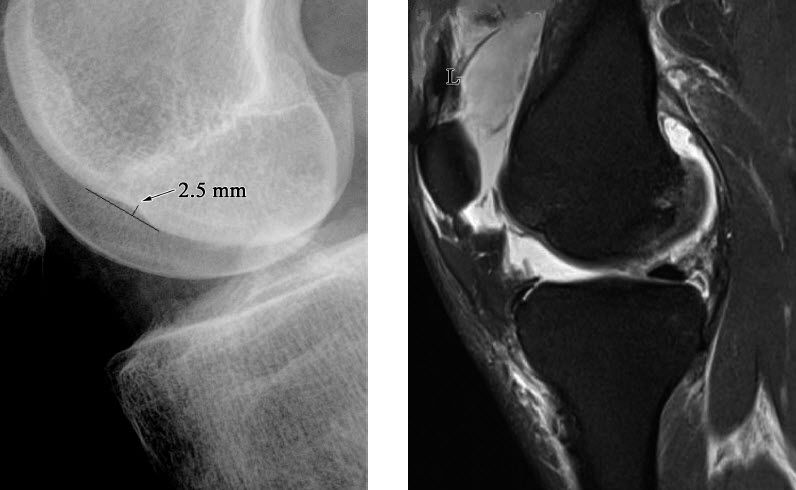
\includegraphics{./images/Image00050.jpg}
 \captionsetup{justification=centering}
 \caption{图2-3-22的放大图}
 \label{fig2-3-23}
  \end{figure} 

标准的侧位片示股骨外侧髁关节面不光整,中央可见局限性凹陷,形成深沟征,沿深沟两点作关节面的切线,再向深沟的最低点作垂线,若垂直线的距离大于2mm,则诊断为深沟征,提示前交叉韧带撕脱性骨折。矢状位T\textsubscript{2}
WI证实X线上股骨外侧沟的深沟征。

有时X线片撕脱性骨折碎片较小不易发现,但临床症状比较明显,此时应进一步行MRI检查。MRI检查对前交叉韧带损伤的敏感性和特异性明显提高,不仅可显示前交叉韧带损伤的具体位置和程度,而且对一些特异性征象,如空窝征(韧带附着处仅见积液无韧带),关节腔内的碎骨片以及对吻损伤(股骨外侧髁和胫骨平台后外侧部骨髓水肿损伤)显示更加明确。可以完全评估损伤的程度,为临床诊断和治疗提供更为精确的依据。

\subsection{腓骨小头骨折}

\begin{figure}[!htbp]
 \centering
 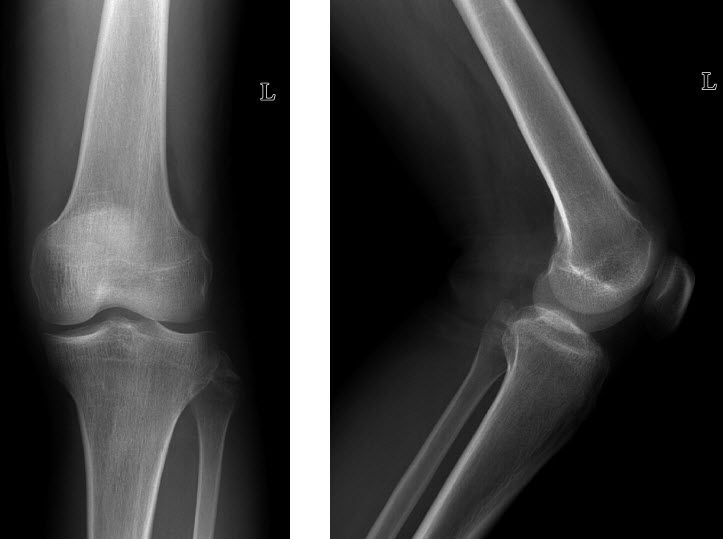
\includegraphics{./images/Image00051.jpg}
 \captionsetup{justification=centering}
 \caption{左膝关节正侧位}
 \label{fig2-3-24}
  \end{figure} 

\textbf{【病史摘要】}
 男性,37岁。上楼时不小心碰到楼梯缘,直接撞伤左膝外侧缘,感剧痛,不能行走。

\textbf{【X线表现】}
 左膝关节正位片示腓骨小头见骨折透亮线影,周边软组织稍肿胀,胫骨平台外侧缘局限性骨密度减低,侧位片示腓骨小头不完全性骨皮质断裂。

\textbf{【X线诊断】}  左侧腓骨小头骨折。

\textbf{【评  述】}
 腓骨小头骨折是一种膝关节比较隐蔽性的骨折。因为胫腓骨比较表浅,易遭受暴力损伤导致骨折,临床上以胫腓骨双骨折比较常见,单纯的腓骨小头骨折比较少见。其骨折机制是腓骨小头遭受侧方暴力直接撞击膝关节所致。在X线正侧位片上大部分腓骨可显示,仅小部分腓骨小头位于胫骨垂直投影侧,容易漏诊。腓骨小头是膝关节外侧副韧带、肱二头肌肌腱和腘腓韧带的止点,对膝关节的稳定起重要作用,因此腓骨小头骨折会导致膝关节慢性不稳,另外腓骨小头骨折可导致腘动静脉损伤或腓总神经的损伤,因此腓骨小头骨折一定要重视,明确检查,了解是否并发膝关节韧带损伤或神经血管损伤。

若X线检查不能明确诊断时,尽早行CT三维重建明确骨折,MRI检查具有更高的特异性和敏感性,在对周边软组织损伤,尤其是在关节韧带、神经损伤的鉴别诊断上更加准确。

\subsection{腓肠豆综合征}

\begin{figure}[!htbp]
 \centering
 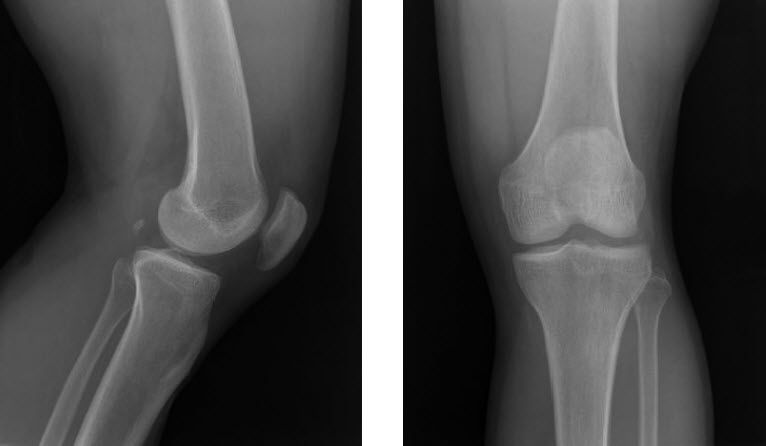
\includegraphics{./images/Image00052.jpg}
 \captionsetup{justification=centering}
 \caption{左膝关节正侧位}
 \label{fig2-3-25}
  \end{figure} 

\textbf{【病史摘要】}  男性,37岁。左膝关节后方反复疼痛。

\textbf{【X线表现】}
 左膝关节侧位片示左膝关节后缘近腘窝处见点状高密度籽骨影,病灶较小,边缘模糊,正位片显示欠佳。

\textbf{【X线诊断】}  左膝腓肠豆综合征。

\textbf{【评  述】}
 腓肠豆是腓肠肌外侧头内的一块籽骨,腓肠豆异常时常引发膝关节后方间歇性疼痛,引起腓肠豆综合征(Fabellar
syndrome)。其最常见原因为青少年运动时直接踢伤或踢球时用力过猛,或腓肠豆和股骨后外侧髁局部反复摩擦所致。腓肠豆综合征主要表现为膝部后外侧间歇性疼痛,关节伸展时疼痛加重,压迫腓总神经,诱发腘窝外侧及小腿腓肠外侧发麻、酸痛,不能久蹲,重则拇趾背伸无力。X线表现为股骨外侧髁后缘软组织内高密度影,密度高于周边软组织,与股骨皮质密度类似,籽骨大小不定,有时较大,形状欠规则。发病机制可能与股骨外侧髁后缘软骨或软骨下改变有关,表现为股骨外侧髁的骨软骨的部分缺失或剥离。若X线不能明确时,可行CT三维检查以进一步明确诊断。

\begin{figure}[!htbp]
 \centering
 \includegraphics{./images/Image00053.jpg}
 \captionsetup{justification=centering}
 \caption{左膝关节CT横断位和矢状位}
 \label{fig2-3-26}
  \end{figure} 

CT横断位和矢状位分别展示了左膝关节股骨外侧髁后方点状高密度灶,另一幅横断位展示股骨外侧髁部分缺损,提示籽骨可能来源于股骨外侧髁的骨软骨的部分剥离。T\textsubscript{2}
WI示股骨外侧髁压脂后呈小片状高信号,提示腓肠豆综合征导致股骨外侧髁的部分炎性水肿。

因此,CT扫描包括三维重建及MRI不仅可明确病灶的位置、大小等,还可明确腓肠豆综合征发生的病因和导致的损伤(尤其是MRI可诊断骨、关节以及软骨的损伤)。

\subsection{髌骨脱位}

\begin{figure}[!htbp]
 \centering
 \includegraphics{./images/Image00054.jpg}
 \captionsetup{justification=centering}
 \caption{膝关节正侧位}
 \label{fig2-3-27}
  \end{figure} 

\textbf{【病史摘要】}
 女性,41岁。上楼梯时被绊倒、跪地,右膝关节疼痛,活动障碍,浮髌征阳性。

\textbf{【X线表现】}
 右侧髌骨向外移位,髌骨超出股骨髁缘2/3,关节囊肿胀(箭头)。

\textbf{【X线诊断】}  右侧髌骨脱位。

\textbf{【评  述】}
 本例为创伤性髌骨脱位,发病机制多为股四头肌的股内侧肌与股四头肌内侧扩张部因外伤撕裂而引起髌骨向外脱位,在X线正位片上表现为髌骨移位于股骨外髁的外侧,MR检查可以清晰地显示髌骨关节半脱位、膝关节积液、股骨髁软骨损伤及其他关节内结构(包括韧带、肌肉)损伤等。本病需要与习惯性髌骨脱位鉴别。习惯性髌骨脱位常在膝关节局部结构发育不良的基础上,经轻微的外伤引起,局部结构发育不良包括膝外侧软组织挛缩而内侧松弛、髌韧带附着点偏外侧、股外侧肌止点异常、髌骨发育小而平、股骨髁间凹发育不良、高位髌骨、膝外翻畸形等,多见于青少年及儿童,中年以上发病较少。

\subsection{踝部外展型三踝骨折}

\begin{figure}[!htbp]
 \centering
 \includegraphics{./images/Image00055.jpg}
 \captionsetup{justification=centering}
 \caption{踝关节正侧位}
 \label{fig2-3-28}
  \end{figure} 

\textbf{【病史摘要】}
 男性,42岁。车祸撞伤左脚踝,左踝关节不能活动,周围软组织肿胀、压痛。

\textbf{【X线表现】}
 左外踝见斜行透亮线影,内踝基底部见横行透亮线影,后踝见纵行透亮线影(箭头)。

\textbf{【X线诊断】}  左踝部外展型三踝骨折。

\textbf{【评  述】}
 踝关节由胫、腓骨下端及距骨组成,构成滑车关节,是一个比较稳定的关节。踝关节骨折是最常见的关节内骨折,可累及一踝、双踝、三踝(胫骨后缘),骨折线可分横行、斜行、螺旋形或纵行,主要为较严重的间接暴力引起。其中三踝骨折可分为四种不同形式:①外旋骨折:内踝骨折线位于基底部或内踝尖端撕脱性骨折,骨折线为斜行或螺旋形,由内上方斜向外下方,在侧位片上较易观察,可合并胫骨后缘骨折和距骨脱位。②外展骨折:内踝骨折线位于基底部,为横行骨折线;外踝骨折线为斜行,位于内踝骨折线的同一水平或腓骨尖端上方数厘米处;后踝骨折线位于胫骨下端后方,为纵行骨折线。③内收骨折:内踝骨折线为垂直或斜行,外踝骨折线位于踝关节水平的横行骨折或为外踝尖端的撕脱骨折。④压缩骨折:踝部压缩骨折由严重的自上而下的重压导致,包括距骨前方半脱位、胫骨前缘纵行骨折、双踝骨折等。本病常伴有胫距后韧带损伤,MR检查表现为韧带增粗,信号异常。

\subsection{距骨后突骨折}

\begin{figure}[!htbp]
 \centering
 \includegraphics{./images/Image00056.jpg}
 \captionsetup{justification=centering}
 \caption{踝关节正侧位}
 \label{fig2-3-29}
  \end{figure} 

\textbf{【病史摘要】}
 女性,38岁。下楼时踏空从楼梯上摔下,右踝扭伤、畸形,关节不能活动。

\textbf{【X线表现】}  右侧距骨后突见裂隙影,骨片轻度下移(箭头)。

\textbf{【X线诊断】}  右侧距骨后突骨折。

\textbf{【评  述】}
 距骨骨折可分为距骨头、颈、体及后突骨折四种类型。后突骨折多为暴力经足跟向上传导或足强力过度跖屈、跟骨向上嵌压时发生。距骨血供不充足,骨折可损伤距骨营养血管,易引起较严重的骨折后不愈合、骨性关节炎及骨缺血性坏死。

鉴别诊断:①先天性距骨后三角副骨,表现为边缘光滑而锐利,多数呈双侧对称分布。②距骨二次骨化中心,常于8~9岁时与距骨体融合,不融合者形成三角副骨。

\subsection{跟骨粉碎性塌陷型骨折}

\begin{figure}[!htbp]
 \centering
 \includegraphics{./images/Image00057.jpg}
 \captionsetup{justification=centering}
 \caption{跟骨侧位、轴位}
 \label{fig2-3-30}
  \end{figure} 

\textbf{【病史摘要】}  女性,30岁。从高处坠落,右后跟着地。

\textbf{【X线表现】}  右侧跟骨见多发骨折碎片,关节面塌陷(箭头)。

\textbf{【X线诊断】}  右侧跟骨粉碎性塌陷型骨折。

\textbf{【评  述】}
 跟骨骨折多由高处摔下,跟骨着地,垂直暴力从距骨传导至跟骨,造成跟骨压缩或劈开,其最常见的合并症是足弓塌陷,距下关节狭窄,凹凸不平,关节面硬化,功能障碍,还可逐渐转化为严重的骨质疏松。对临床怀疑跟骨骨折,除正侧位观察外,轴位有时也是必要的,以免骨折线和移位不明显的跟骨骨折漏诊。需鉴别塌陷型与部分碎裂型跟骨骨折:前者骨折线常影响距骨下关节面,根据塌陷情况又可分为外侧距骨下关节塌陷和全部距骨下关节塌陷;后者骨折线不累及距骨下关节面,愈合较好。

大约75%跟骨骨折的患者其骨折延伸至跟距关节。有时轻微的凹陷型骨折不易被显示,可通过观察跟距角的减小来提示诊断。当跟距角即Bohler's角(侧位片上从跟距关节最高点到跟骨前突和跟骨后上面分别连线之间的夹角)小于28°时诊断为跟距关节下移。

\subsection{跖骨骨折}

\begin{figure}[!htbp]
 \centering
 \includegraphics{./images/Image00058.jpg}
 \captionsetup{justification=centering}
 \caption{足正斜位}
 \label{fig2-3-31}
  \end{figure} 

\textbf{【病史摘要】}
 女性,47岁。搬家时重物砸伤左足背,足背肿胀、疼痛。

\textbf{【X线表现】}
 左足第2、5跖骨基底部见透亮线影,对位、对线良好(箭头)。

\textbf{【X线诊断】}  左足第2、5跖骨基底部骨折。

\textbf{【评  述】}
 跖骨骨折多因扭伤、车轮压伤或重物直接撞击所致,分为基底部、骨干及颈部骨折,其中基底部骨折最多见,骨干部次之,颈部最少,常为几个跖骨同时发生,但第2跖骨和第5跖骨基底部常可单独发生。跖骨亦可发生疲劳性骨折,多发生在跖骨中段或上、中1/3交界段,长期、反复的外力集中作用于此,逐渐形成慢性骨折,2~3周后可有骨痂形成,呈典型的梭形隆起,其中可见致密线。需与第5跖骨基底部骨骺鉴别,后者大致9岁出现,15~16岁愈合,骨骺呈鳞片状,骺线纵行。

跖骨骨折常伴发跗跖关节脱位,跗跖关节脱位在X线诊断时很容易遗漏,因此必须熟悉正常的关节对合关系。如正位片上第2跖骨基底部内侧缘与中间楔骨内侧缘呈直线对应关系;斜位片上第3跖骨基底部内侧缘与外侧楔骨内侧缘呈直线;如发现4块跖骨的基底部骨折,应同时注意有无关节脱位。需要注意的是糖尿病患者神经关节病常表现为慢性跗跖关节脱位。

跖骨是很容易发生疲劳骨折的部位,疲劳骨折是由于超负荷承重反复作用于正常骨质导致的一种应力性骨折,疲劳骨折患者主要跟从事活动性质有关,多见于训练中的运动员和新兵。疲劳骨折典型的好发部位和原因包括:跖骨干:行军和芭蕾舞;跟骨:初学走路的幼儿;胫骨:初学走路的幼儿,长跑;腓骨远端:长跑;腓骨近端:跳跃;股骨颈、股骨干:芭蕾舞,体操和长跑;脊椎椎弓峡部:芭蕾舞,举重和清洁工;肋骨:咳嗽,携重物;下位颈椎或上位胸椎棘突:挖掘,耕作。

若骨折线不能被X线所发现,MRI或核素检查常为阳性,可提供早期诊断。但是在对应力性骨折的评价中,MRI相对于核素扫描来说诊断敏感性相似,但特异性较高。

\subsection{椎体压缩性骨折}

\begin{figure}[!htbp]
 \centering
 \includegraphics{./images/Image00059.jpg}
 \captionsetup{justification=centering}
 \caption{腰椎正侧位}
 \label{fig2-3-32}
  \end{figure} 

\textbf{【病史摘要】}
 男性,33岁。被汽车撞后,腰背部疼痛,背部压痛明显,活动时加剧。

\textbf{【X线表现】}
 腰1椎体变扁,呈楔形改变,前缘及上缘骨皮质不连续(箭头)。

\textbf{【X线诊断】}  腰1椎体压缩性骨折。

\textbf{【评  述】}
 椎体压缩性骨折,多数为间接暴力,如从高处落下;少数为直接暴力,如交通事故直接撞击;还可由肌肉拉力所致的病理性骨折。最常见的X线征象为椎体呈楔形变,前缘压缩明显,后缘压缩较轻;较少见的征象可以为椎体横径稍增宽,椎体上部骨质内见压缩而致骨小梁排列紊乱的致密带;最少见的征象为椎体没有压缩而在边缘出现斜行或横行骨折线或小片骨撕裂。需要与骨质疏松及病理性原因引起的椎体压缩性骨折鉴别。骨质疏松引起的椎体压缩性骨折X线表现为椎体普遍性骨质疏松,椎体上、下缘呈双凹变形,多见于老年女性和内分泌紊乱患者;病理性原因引起的椎体压缩性骨折X线表现为一个或多个椎体有骨质破坏,常累及椎体后部、椎弓及附件,老年人多为转移瘤。

椎体骨折最常见的位置依次为:C1~C2(上颈椎)、C5~C6(下颈椎)、T10~T12(胸腰段)。不仅20%为多发骨折,而且85%的患者会并发脊髓损伤。

椎体骨折的平片需要诊断4个主要特征:①骨折的水平或位置;②有无明显移位(对线关系);③脊柱的稳定性;④骨折的时间(陈旧性骨折、新鲜骨折、混合性骨折)。

\subsection{寰枢关节脱位}

\begin{figure}[!htbp]
 \centering
 \includegraphics{./images/Image00060.jpg}
 \captionsetup{justification=centering}
 \caption{颈椎张口位}
 \label{fig2-3-33}
  \end{figure} 

\textbf{【病史摘要】}
 男性,41岁。急刹车时头一侧撞击在车厢上,头颈部不能旋转,疼痛。

\textbf{【X线表现】}
 齿状突偏位,寰椎两侧侧块与齿状突形成的关节间隙不对称(箭头)。

\textbf{【X线诊断】}  寰枢关节脱位。

\textbf{【评  述】}
 寰枢关节为轴承状关节,可使头部产生旋转运动,正常时齿状突位于寰椎两侧块中央。寰枢关节脱位的暴力多为头部过度前屈所致,常合并齿状突骨折及韧带损伤,严重时可损伤脊髓和延髓,摄片时应尽量避免过度搬动头颈部。X线张口位及CT多平面重建能观察寰枢关节脱位。

鉴别诊断:①齿状突偏位,与寰椎两边侧块的间距不等宽。②寰枢椎关节间隙增宽,成人超过3mm、儿童超过4mm。③脊椎椎管前后缘连线及棘突连线相错。

张口位、侧位和前后位是可疑颈椎骨折的最常用的三个摄片体位。由于韧带损伤可能,急诊就诊患者不准摄伸颈和屈颈位侧位片。如果常规X线平片隐性,CT检查可以发现隐匿性骨折,MRI则可以发现韧带损伤。

齿突骨折分型:①Ⅰ型:齿突上部骨折(稳定型);②Ⅱ型:齿突基底部骨折(不稳定型);③Ⅲ型:齿突基底部骨折累及椎体(稳定型,预后较好)。

\subsection{骨盆骨折}

\begin{figure}[!htbp]
 \centering
 \includegraphics{./images/Image00061.jpg}
 \captionsetup{justification=centering}
 \caption{骨盆正位}
 \label{fig2-3-34}
  \end{figure} 

\textbf{【病史摘要】}  男性,34岁。被撞倒后,骨盆疼痛,不能活动。

\textbf{【X线诊断】}
 双侧耻骨上下支、左侧髋臼见透亮线影,左侧骶髂关节间隙增宽,耻骨联合间隙增宽(箭头)。

\textbf{【X线诊断】}  骨盆环多发骨折伴左侧骶髂关节脱位、耻骨联合分离。

\textbf{【评  述】}
 骨盆是一个坚强的骨环,由骶骨、髂骨、坐骨和耻骨联合组成。骨盆骨折多由直接暴力挤压骨盆所致,多见于交通事故和塌方,也可因肌肉强烈收缩引起骨盆的骨突撕脱骨折,常合并内部脏器损伤,如膀胱、直肠、尿道、大血管及神经损伤等,严重者出现创伤性失血性休克,危及生命。根据骨折与骨盆环的结构关系分为骨盆环骨折、骨盆边缘骨折及骨盆撕脱性骨折。

一般X线平片多可诊断,CT及MR检查主要用于观察骨盆脏器受损情况。X线检查需要鉴别单发骨折和多发骨折:前者主要发生在骨盆环状结构中,某一处骨折使骨盆环中断,骨折端多无移位,骨盆仍保持稳定;后者发生在两处以上,骨折端有明显移位,可同时伴有骶髂关节脱位和耻骨联合分离,骨盆的稳定性遭到破坏。

\section{骨缺血性坏死及骨软骨病}

\subsection{股骨头骨骺缺血性坏死}

\begin{figure}[!htbp]
 \centering
 \includegraphics{./images/Image00062.jpg}
 \captionsetup{justification=centering}
 \caption{右髋正位}
 \label{fig2-4-1}
  \end{figure} 

\textbf{【病史摘要】}  女性,8岁。右髋关节疼痛不适4个月。

\textbf{【X线表现】}
 右侧股骨头骨骺变扁,骨骺密度增高,不均匀,内见密度减低区,髋关节间隙增宽,股骨颈缩短、增粗。

\textbf{【X线诊断】}  股骨头骨骺缺血性坏死。

\textbf{【评  述】}
 本病又称扁平髋,多见于5~10岁儿童,常为单侧,亦可为双侧。30%有外伤史。好发于股骨头的前外侧,逐渐累及全骺。早期骨质改变不明显,关节囊软组织肿胀,股骨头骨骺较健侧小,密度均匀性增高。进展期股骨头内出现节裂及小囊性变。晚期股骨头出现蕈样或圆帽状畸形,骨骺碎裂,股骨颈短粗,大粗隆升高,颈干角变小,形成髋内翻。常可继发退行性骨关节病改变。

鉴别诊断:①化脓性髋关节炎:发病急,症状重,股骨头的关节面关节软骨首先发生变化,骨质破坏迅速,晚期常有关节骨性强直。②髋关节结核:股骨头骨骺局限性骨质破坏,随后骨骺进行性骨破坏,股骨颈外形无明显改变,骨质疏松广泛,髋臼受累破坏,晚期可见纤维性强直。③先天性髋内翻:病史明确,脱位明显,髋内翻,髋臼小,股骨颈不增粗,股骨头向下移位。

\subsection{成人股骨头缺血性坏死}

\begin{figure}[!htbp]
 \centering
 \includegraphics{./images/Image00063.jpg}
 \captionsetup{justification=centering}
 \caption{双髋正位}
 \label{fig2-4-2}
  \end{figure} 

\textbf{【病史摘要】}
 男性,49岁。左髋关节疼痛6个多月,关节活动障碍,行走困难。下肢有缩短、外展。

\textbf{【X线表现】}
 左侧股骨头形态不规则,骨质破坏区内见片状致密影,骨小梁结构模糊,股骨颈变短、变粗,髋臼上缘关节面密度增高。

\textbf{【X线诊断】}  左侧股骨头缺血性坏死。

\textbf{【评  述】}
 多数患者有长期或大量应用类固醇激素史,另外髋关节外伤、糖尿病和酗酒者以及放疗后患者也可引发本病。X线表现早期股骨头骨小梁模糊,轻度骨质疏松,以后逐渐出现斑片状骨质硬化及不规则透亮区,大块骨碎裂、塌陷,股骨头碎解、吸收,重者股骨头可消失,颈部成为关节端。晚期可引起继发性退行性骨关节病及关节间隙变窄。脱落的骨片可形成关节游离体。髋臼可发生相对的关节面下骨增生改变。本病主要应与化脓性关节炎、关节结核进行区别。后两者多为溶骨性破坏,髋臼同时受累。化脓性关节炎发病急,症状重,骨破坏迅速,周围骨增生明显,晚期可发生骨性强直。结核病程长,骨质疏松广泛,病变周围无骨增生现象,骨破坏广泛,多见于青少年。

\subsection{椎体缺血性坏死}

\begin{figure}[!htbp]
 \centering
 \includegraphics{./images/Image00064.jpg}
 \captionsetup{justification=centering}
 \caption{胸椎侧位}
 \label{fig2-4-3}
  \end{figure} 

\textbf{【病史摘要】}
 男性,6岁。腰背疼痛2年,胸腰段有轻度驼背,无其他特殊症状,胸椎有压痛。

\textbf{【X线表现】}
 胸T12椎呈扁平状,前后径增加,密度增高,椎间隙正常。其周围未见软组织肿块,椎弓未见破坏。

\textbf{【X线诊断】}  椎体缺血性坏死。

\textbf{【评  述】}
 本病系椎体一次骨化中心缺血坏死所致,亦称扁平椎、铜板椎,最常见的是由嗜酸性肉芽肿引起。多见于2~15岁儿童,好发下胸椎,单个椎体多见,也可多发。临床症状可伴有脊柱后突畸形。典型者椎体X线上呈盘状或铜钱状,椎体前后径及横径增大,椎间隙多增宽,少累及椎弓根。病变椎体可逐渐恢复或接近正常,后突畸形可逐渐纠正。

鉴别诊断:①脊柱结核:多有肺结核,病变累及多个椎体,椎体密度减低、破坏,椎间隙变窄、消失,其周围见寒性脓肿。②椎体病理性骨折:原有病变,多累及椎体附件。

\subsection{月骨骨软骨病}

\begin{figure}[!htbp]
 \centering
 \includegraphics{./images/Image00065.jpg}
 \captionsetup{justification=centering}
 \caption{腕关节正位}
 \label{fig2-4-4}
  \end{figure} 

\textbf{【病史摘要】}
 男性,30岁。右腕疼痛10个月,活动障碍,握力下降,局部有压痛。

\textbf{【X线表现】}
 月骨正常骨小梁结构消失、模糊,呈明显不均匀异常高密度,周围关节间隙尚可。

\textbf{【X线诊断】}  月骨缺血性坏死。

\textbf{【评  述】}
 本病好发年龄为20~30岁,男性多于女性,右手较左手多5倍,常发生于重手工劳动者,临床以疼痛为主,活动受限,局部压痛。月骨X线表现为密度增高,外形扁平、不规则,见有裂隙或小囊变,邻近关节间隙正常或稍宽。晚期月骨密度趋向正常,骨小梁再现,但骨外形不能恢复。常合并退行性关节病。

鉴别诊断:①月骨骨折:有明确外伤史及骨折线。②腕关节结核:以骨质破坏为主,累及关节及其他腕骨。③二分手舟骨:为先天变异,表现为双侧发生,骨块边缘光滑,骨小梁正常,临床无症状。

\subsection{跖骨头缺血性坏死}

\begin{figure}[!htbp]
 \centering
 \includegraphics{./images/Image00066.jpg}
 \captionsetup{justification=centering}
 \caption{足正位}
 \label{fig2-4-5}
  \end{figure} 

\textbf{【病史摘要】}
 女性,24岁。第3跖趾关节疼痛1年,活动后加重,曾有外伤史。

\textbf{【X线表现】}
 第3跖骨头扁平、增宽,中央有凹陷,密度增高、不均。对应趾骨关节面边缘呈唇样骨质增生、硬化,关节间隙狭窄。

\textbf{【X线诊断】}  第3跖骨头缺血性坏死。

\textbf{【评  述】}
 好发于10~20岁青少年,女性多于男性。多见于第2跖骨头,偶见于第3跖骨头。以局部肿胀、疼痛、压痛、活动加重、行走困难为主要症状。早期第2跖骨头密度增高,关节面变平、不规则或碎裂,其下方的骨质出现骨质疏松和节裂。随病变发展,跖骨头增宽,中央凹陷呈喇叭状,其内可见不规则游离体,相对应的跖骨基底部也发生骨质增生。晚期可发生退行性骨关节病。

鉴别诊断:①跖骨远端陈旧性骨折:有明显外伤史及关节肿痛。②跖趾关节炎:早期关节红肿、热痛明显,关节间隙增宽;晚期骨质增生明显,关节面变形,关节间隙变窄。

\subsection{椎体骺板软骨病}

\begin{figure}[!htbp]
 \centering
 \includegraphics{./images/Image00067.jpg}
 \captionsetup{justification=centering}
 \caption{腰椎侧位}
 \label{fig2-4-6}
  \end{figure} 

\textbf{【病史摘要】}
 女性,12岁。腰背部疼痛1年余,有疲劳感,直立时酸胀明显,卧位休息可缓解。

\textbf{【X线表现】}
 L2、L3椎体终板不规则,L3前缘可见许莫氏结节,L2/3椎间隙狭窄。

\textbf{【X线诊断】}  L2、L3椎体骺板骨软骨病。

\textbf{【评  述】}
 本病又称青年驼背症,好发于12~18岁青少年,男性为女性的4~5倍。主要临床表现为驼背,腰背部疼痛,卧床休息后好转。主要病变是椎体环骺缺血性坏死和软骨疝。常累及多个椎体,以负重大的下胸段至上腰段为好发部位。主要X线表现为椎体骨骺出现延迟并呈现疏松、分节、密度增高、轮廓不清。椎体和环骺间匀称透明线不规则增宽,椎间盘变窄,椎体前部可呈不规则毛糙、凹陷,上下缘阶梯状凹陷,常有许莫氏结节形成。多个椎体楔形变使脊柱后突畸形,呈圆背状后突或侧突,椎间隙多正常。恢复期,椎骺与椎体融合,椎间隙可变窄,椎体变形及永久性驼背,常合并脊椎退行性骨关节病。椎体骺板骨软骨病需要在概念上与椎体终板骨软骨炎相区别。虽然两者都指软骨缺血坏死,但它们所指的解剖部位不一样,前者是在骨骺未与椎体融合时存在,因此它通常发生于青少年,缺血坏死后椎体会发生楔形变;而终板是椎体和椎间盘相邻近的一层薄软骨板,椎体终板终生存在,而且终板骨软骨炎又是发生于椎间盘退变的基础上,一般发生于中老年人,此时椎体骨骺已经和椎体融合,骺板消失,因此它不发生楔形变。

\subsection{胫骨结节骨软骨病}

\begin{figure}[!htbp]
 \centering
 \includegraphics{./images/Image00068.jpg}
 \captionsetup{justification=centering}
 \caption{膝关节侧位}
 \label{fig2-4-7}
  \end{figure} 

\textbf{【病史摘要】}
 男性,16岁。右膝疼痛1年,其周围软组织肿胀,压痛明显。

\textbf{【X线表现】}
 右侧胫骨结节密度不均匀,见部分碎裂致密骨片(箭头),胫骨结节下方与骨干分离。膝关节面未见异常。

\textbf{【X线诊断】}  右侧胫骨结节骨软骨病。

\textbf{【评  述】}
 本病好发于10~15岁男性,与剧烈运动和外伤有关,多为单侧,亦可为双侧,患部肿胀、疼痛、压痛,形成胫骨结节的唇状骨骺4~11岁出现,20岁与胫骨干联合。X线主要表现早期为局部软组织肿胀,以髌韧带的增大、增厚为特征。胫骨结节密度增高,呈碎裂状并与骨干分离,相应干骺端常出现对应的骨缺损。晚期骨质可恢复正常或有骨性隆起,碎片亦可存留在髌韧带内。

鉴别诊断:①胫骨结节正常变异:胫骨结节骨骺唇状骨突在发展过程中出现两个或两个以上骨化中心,表现为一个或多个边缘光滑、间隙匀称的骨块,多位于髌韧带的屈侧,局部压痛、X线片上软组织肿胀、髌韧带局限性增厚突出现象是本病诊断要点。②撕脱性骨折:有明确外伤史,局部剧痛及肿胀,游离骨块部分边缘毛糙不齐并明显移位。

\subsection{耻骨骨软骨炎}

\begin{figure}[!htbp]
 \centering
 \includegraphics{./images/Image00069.jpg}
 \captionsetup{justification=centering}
 \caption{骨盆正位}
 \label{fig2-4-8}
  \end{figure} 

\textbf{【病史摘要】}
 女性,21岁。耻骨联合处疼痛1个月,休息后缓解,局部有压痛,活动受限,皮肤无红肿。

\textbf{【X线表现】}  耻骨联合明显增宽,双侧耻骨缘呈鼠咬状,密度增高。

\textbf{【X线诊断】}  耻骨骨软骨炎。

\textbf{【评  述】}
 本病又称非化脓性耻骨炎、耻骨联合关节炎,好发于男性泌尿系统术后以及30岁以下的孕、产妇及某些项目的运动员。临床表现为单侧及双侧耻骨联合部剧痛和局限性压痛,病程有自限性趋势,数月或数年后自愈。本病X线表现与临床症状不同步,症状出现或消失均早于骨改变。X线主要表现为耻骨联合间隙有不同程度的增宽(0.6~4.8cm)。耻骨缘骨质可见纵行透亮区,耻骨局限性骨密度增高,一侧或双侧耻骨呈鼠咬状骨质破坏,严重者其边缘呈多弧形切迹,边缘锐利,可有碎裂骨片。数个月或数年后可自愈。

鉴别诊断:①耻骨结核:多呈囊状破坏,内见沙粒样死骨,周围骨质疏松,耻骨变形,易形成脓肿或瘘管。②化脓性骨髓炎:局部红肿、热痛,常单侧发病,一般不累及对侧耻骨,骨质破坏与增生均较广泛,骨膜反应明显,痊愈后往往留有骨密度增高和结构紊乱现象。

\subsection{髂骨致密性骨炎}

\begin{figure}[!htbp]
 \centering
 \includegraphics{./images/Image00070.jpg}
 \captionsetup{justification=centering}
 \caption{骨盆正位}
 \label{fig2-4-9}
  \end{figure} 

\textbf{【病史摘要】}  女性,29岁。两侧骶髂关节疼痛6个月。

\textbf{【X线表现】}
 两侧骶髂关节髂骨缘中下部见片状致密影,骨小梁消失,外侧边缘模糊,关节面未见破坏,关节间隙正常。

\textbf{【X线诊断】}  两侧髂骨致密性骨炎。

\textbf{【评  述】}
 本病多发生于20~25岁女性。与妊娠、慢性劳损和泌尿系统感染有关,有自限性,50岁以后很少有此病。本病绝大多数发生在髂骨耳状面,经产妇和站立工作者发病较高。髂骨耳状面中下2/3出现三角形、半月形的均匀致密影,内缘达骶髂关节面,外缘与正常骨移行界限不清,关节间隙正常,无骨质破坏。本病与结核性骶髂关节炎、强直性脊柱炎、低毒性骶髂关节炎的鉴别要点为关节间隙正常、关节面光整、无骨质破坏。

\section{骨及关节化脓性感染}

\subsection{急性化脓性骨髓炎}

\begin{figure}[!htbp]
 \centering
 \includegraphics{./images/Image00071.jpg}
 \captionsetup{justification=centering}
 \caption{肱骨正侧位}
 \label{fig2-5-1}
  \end{figure} 

\textbf{【病史摘要】}
 男性,15岁。左侧上肢胀痛1周,伴发热、寒战,活动障碍。体格检查:左上臂软组织红肿明显,皮温高,并有压痛。

\textbf{【X线表现】}
 上臂软组织肿胀,肌间隙模糊,肱骨干骺端见斑片状骨质破坏,骨干见线样骨膜反应,中上段骨松质及骨皮质密度不均匀。

\textbf{【X线诊断】}  左肱骨上段急性化脓性骨髓炎。

\textbf{【评  述】}
 好发于儿童和青少年,多为男性,以胫骨、股骨、肱骨、桡骨等长管骨的干骺端为常见。起病急,寒战、高热等全身中毒症状明显,局部红、肿、热、痛,压痛,血象增高。特点为骨改变的X线表现晚于临床表现。骨破坏与骨增生并存。早期仅表现为软组织肿胀。发病1~2周后,干骺端斑片状或大片状低密度区,迅速向骨干蔓延,骨皮质呈筛孔样、虫蚀样不规则低密度或中断消失,常合并病理性骨折。骨膜反应明显,与病变范围一致。严重者病变区可见与长轴一致长方形密度更高的死骨,周围密度较低,边界清楚。病变可侵犯关节。

鉴别诊断:①尤文肉瘤:本病多位于骨干,少数位于干骺端及骨骺,髓内生长,破坏皮质,可见软组织肿块。②骨肉瘤:可见软组织肿块及瘤骨。急性化脓性骨髓炎有时也表现为粗或细的骨针,甚至出现Codemn三角,与骨肉瘤鉴别较难,因此了解患者病史对诊断非常重要。

\subsection{慢性化脓性骨髓炎}

\begin{figure}[!htbp]
 \centering
 \includegraphics{./images/Image00072.jpg}
 \captionsetup{justification=centering}
 \caption{尺桡骨侧位}
 \label{fig2-5-2}
  \end{figure} 

\textbf{【病史摘要】}
 男性,8岁。左前臂肿胀1年伴流脓2个月,肢体有弯曲畸形。体格检查:左前臂软组织肿胀,皮肤温度稍高,见窦道。

\textbf{【X线表现】}
 左桡骨全段骨质破坏,皮质不规则增厚,骨髓腔狭窄,骨破坏区内见长条形死骨。骨干变形,周围软组织明显肿胀。

\textbf{【X线诊断】}  慢性化脓性骨髓炎。

\textbf{【评  述】}
 本病临床表现较急性轻,X线主要表现以骨质增生为主,表现为骨质硬化,骨膜新生骨增生显著,形成骨包壳,骨干增粗,髓腔消失,可见脓腔及死骨、窦道。经久不愈的窦道可引发类上皮癌。在增粗及增厚的皮质边缘突然出现线样骨膜反应提示急性发作。慢性化脓性骨髓炎愈合标准:脓腔及死骨消失,病变区密度均匀性增高,并逐渐出现骨小梁。

鉴别诊断:①结核性骨髓炎:一般多侵入关节,病史较缓慢,有结核病或结核病接触史等,其典型的X线片显示以骨质破坏为主而少有新骨形成。②后天获得性梅毒:鉴别要点为骨内膜和骨膜新生骨导致长骨硬化增厚,内可见边界模糊的溶骨性骨质破坏灶(梅毒树胶肿)是其特征性改变。

大约有1%的慢性化脓性骨髓炎患者在慢性排脓的窦道口发生表皮样癌,X线表现为软组织肿块显著增大,并且侵蚀病骨,此时要引起高度重视。

\subsection{慢性局限性骨脓肿}

\begin{figure}[!htbp]
 \centering
 \includegraphics{./images/Image00073.jpg}
 \captionsetup{justification=centering}
 \caption{股骨正位(局部放大)}
 \label{fig2-5-3}
  \end{figure} 

\textbf{【病史摘要】}
 女性,17岁。右股骨下端疼痛1个月余。体格检查:股骨下端局限性压痛,其周围软组织未见异常。

\textbf{【X线表现】}
 股骨下段见圆形透亮区,边缘光整,其周围骨密度增高,骨小梁模糊。

\textbf{【X线诊断】}  慢性局限性骨脓肿。

\textbf{【评  述】}
 本病为慢性局限性低毒性感染,好发于胫骨上下端、股骨上端干骺端。临床症状轻微,以疼痛为主,呈阵发性、夜间加重。X线表现:骨干骺端中心或偏一侧见类圆形低密度影,边界清楚,周围骨质增生硬化带,边缘移行。骨外形一般无改变,一般无死骨、骨膜反应和软组织肿胀。如病变发生在边缘或较细骨骼,可见骨膜反应,偶见死骨。

鉴别诊断:①骨样骨瘤:病变发生在骨皮质,引起骨皮质增生硬化。②骨骺、干骺结核:为干骺端边缘清楚的低密度骨质破坏区,易累及骨骺,破坏区周边无硬化带而有骨质疏松。

\subsection{硬化性骨髓炎}

\begin{figure}[!htbp]
 \centering
 \includegraphics{./images/Image00074.jpg}
 \captionsetup{justification=centering}
 \caption{股骨正侧位}
 \label{fig2-5-4}
  \end{figure} 

\textbf{【病史摘要】}
 女性,44岁。右侧股骨下段隐痛,间断性发作。体格检查:右股骨下段压痛,周围软组织未见明显异常。

\textbf{【X线表现】}
 右股骨下段呈梭形增粗,骨皮质增厚,骨髓腔变窄,未见明显骨膜增生反应及骨质破坏。

\textbf{【X线诊断】}  硬化性骨髓炎。

\textbf{【评  述】}
 本病又称干性骨髓炎,是骨组织低毒性感染性疾病。病变处骨质以硬化为主。临床症状轻微,表现为局部的反复疼痛。病骨骨干匀称性梭形增粗,皮质增厚、髓腔狭窄;外缘光整,无骨膜反应。病程较长时,可见不规则斑点状破坏区,常无死骨形成。

鉴别诊断:①硬化性骨梅毒:梅毒性骨膜炎以多发、硬化为特征,两侧对称,而且有性病家族史及螺旋体抗原阳性等。②骨样骨瘤:骨干骨皮质增生,中间见小透亮区。③硬化性骨肉瘤:好发于青少年的干骺端,有放射状增生和骨膜三角存在。④Ribbing病:遗传性多发性骨干硬化,与广泛性硬化骨髓炎鉴别,不同点是前者的典型表现为骨干非对称性增生硬化。

\subsection{脊柱化脓性骨髓炎}

\begin{figure}[!htbp]
 \centering
 \includegraphics{./images/Image00075.jpg}
 \captionsetup{justification=centering}
 \caption{腰椎侧位}
 \label{fig2-5-5}
  \end{figure} 

\textbf{【病史摘要】}
 男性,39岁。咳嗽2个月余,现感“腰部不适”。实验室检查:中性粒细胞计数为7.1×10\textsuperscript{9}
/L。

\textbf{【X线表现】}
 L3下缘及L4椎体上缘终板密度减低,L4终板下椎体密度不均,L3/4椎间隙狭窄(箭头)。

\textbf{【X线诊断】}  L3、L4化脓性骨髓炎。

\textbf{【评  述】}
 本病青壮年多见,以腰椎为多。临床有高热、寒战等败血症史。X线表现分为椎间型、椎体型、骨膜下型和附件型。本病起病急,进展迅速,早期即可引起椎间隙狭窄。X线征象与临床相结合能够准确诊断。本病现已少见。

鉴别诊断:①骨结核:病程缓慢,以骨破坏为主,病变区可见沙砾样死骨或干酪组织钙化,增生硬化及骨桥少见。②转移性肿瘤:病变多累及多椎体及椎弓根,无骨桥形成。

\section{骨及关节结核}

\subsection{骨骺及干骺端结核}

\begin{figure}[!htbp]
 \centering
 \includegraphics{./images/Image00076.jpg}
 \captionsetup{justification=centering}
 \caption{膝关节正位}
 \label{fig2-6-1}
  \end{figure} 

\textbf{【病史摘要】}
 男性,13岁。2年前发现肺结核,正规药物治疗1年余,左侧膝关节隐痛半年,无高热病史,血沉25mm/h。

\textbf{【X线表现】}
 左侧股骨干骺端及骨骺见多发囊状密度减低区,病变跨越干骺端及骨骺,病变中心见死骨,边缘局部轻度增生,未见明显骨膜反应。左侧膝关节间隙增大,周围软组织明显肿胀。

\textbf{【X线诊断】}  左侧股骨干骺端及骨骺结核。

\textbf{【评  述】}
 本病好发于儿童及青少年长骨的干骺端或骨骺。临床一般无全身症状,但是局部破坏严重。X线表现为骨骺及干骺端类圆形或不规则形骨破坏区,边缘较锐利,破坏区可见沙砾样死骨,很少有骨膜反应。病变常向关节方向发展,干骺端结核可穿越骺板进入骨骺形成病灶骑跨骺板现象。

鉴别诊断:①骨囊肿:好发于干骺端中央部,多为卵圆形,边缘清晰锐利,内无死骨。②巨细胞瘤:好发于骨端突出部分,偏心、膨胀性生长,无死骨及周围软组织肿胀。

\subsection{骨干结核}

\begin{figure}[!htbp]
 \centering
 \includegraphics{./images/Image00077.jpg}
 \captionsetup{justification=centering}
 \caption{股骨正侧位}
 \label{fig2-6-2}
  \end{figure} 

\textbf{【病史摘要】}
 男性,19岁。左下肢反复酸痛、无力,近3个月感觉左大腿肿胀,无明显红肿、热痛改变。

\textbf{【X线表现】}
 左股骨上段见局部卵圆形低密度影,边界清晰,一侧骨皮质破坏明显,可见轻度骨膜反应。

\textbf{【X线诊断】}  左股骨上段骨干结核。

\textbf{【评  述】}
 长骨骨干结核较少见,好发于儿童,常见于桡骨、胫骨,为一种局限型慢性结核感染。临床有局部不适、疼痛。重者X线表现为骨干中央呈圆形或卵圆形的破坏区;病变较大侵犯骨皮质时,骨干呈梭形增粗,骨膜增生明显。

鉴别诊断:①慢性局限性骨脓肿:好发于干骺端,在骨质破坏区常伴有广泛的骨质增生,很少有骨膜反应。②非骨化性纤维瘤:多位于骨端,呈单房或分房状膨胀性骨质破坏。

\subsection{短骨结核}

\begin{figure}[!htbp]
 \centering
 \includegraphics{./images/Image00078.jpg}
 \captionsetup{justification=centering}
 \caption{足正斜位}
 \label{fig2-6-3}
  \end{figure} 

\textbf{【病史摘要】}
 男性,25岁。右足第1跖骨肿胀半年余,服用抗炎药治疗无效,近日感觉症状明显,无明显红肿、热痛改变。

\textbf{【X线表现】}
 右足第1跖骨见卵圆形骨质破坏区,边界尚清晰,未见明显骨质增生硬化,周围软组织未见明显异常。

\textbf{【X线诊断】}  右足第1跖骨结核。

\textbf{【评  述】}
 本病又称骨气臌,多见于儿童,双侧发病。病变往往多发,但很少侵犯末节指(趾)骨。早期局部症状轻微,随后病骨周围组织逐渐肿胀,并出现疼痛。病变从骨髓开始,短骨呈梭形增粗。典型的骨气臌及病灶内沙砾样小死骨是诊断的关键。病变一般不侵犯关节。

鉴别诊断:①多发性内生性骨软骨瘤:膨胀性骨质破坏,瘤区内有条状骨嵴,周围无骨硬化及骨膜反应。②痛风:X线片示短管状骨骨端虫蚀状破坏,但无骨膜反应,局部皮肤红肿。

\subsection{脊椎结核}

\begin{figure}[!htbp]
 \centering
 \includegraphics{./images/Image00079.jpg}
 \captionsetup{justification=centering}
 \caption{腰椎正侧位}
 \label{fig2-6-4}
  \end{figure} 

\textbf{【病史摘要】}  男性,28岁。乏力1个月,低热、腰痛2周。

\textbf{【X线表现】}
 腰椎侧弯,L3/4椎间隙明显变窄。侧位片示:生理曲度变直,L3/4椎间隙变窄,L3、L4椎体明显变小,呈融骨性骨质破坏,未见明显骨质硬化。

\textbf{【X线诊断】}  脊椎结核。

\textbf{【评  述】}
 本病在骨关节结核中最常见,占骨关节结核的40%~50%,以青壮年为主。腰椎为最好发的部位,胸椎次之。临床常有腰背部疼痛、脊椎畸形和运动障碍,部分患者可有寒性脓肿形成。X线表现有骨质破坏、椎间隙变窄或消失、后突畸形、死骨和寒性脓肿等征象。

鉴别诊断:①转移瘤:多个椎体及附件见骨质破坏,无椎间盘破坏及寒性脓肿形成,而90%的脊椎结核侵犯椎体,很少累及附件。②椎体压缩性骨折:可见一个或多个椎体楔形变,但是椎间盘间隙无明显变窄。③化脓性脊柱炎:病程进展快,骨质增生硬化明显。

目前X线诊断脊柱结核有以下几个要点:①累及3个或更多椎体。②脊柱内跳跃病灶。③一个大的或钙化的椎旁脓肿。④很少累及椎弓。

\subsection{骶髂关节结核}

\begin{figure}[!htbp]
 \centering
 \includegraphics{./images/Image00080.jpg}
 \captionsetup{justification=centering}
 \caption{骨盆正位}
 \label{fig2-6-5}
  \end{figure} 

\textbf{【病史摘要】}  女性,24岁。左腿痛,左侧臀部肿大,无明显红肿。

\textbf{【X线表现】}  左侧骶髂关节的关节面毛糙、硬化,局部骨质破坏。

\textbf{【X线诊断】}  左侧骶髂关节结核。

\textbf{【评  述】}
 骶髂关节结核常与相邻的腰骶椎或髋关节结核并存,多见于青壮年。起病隐匿,常倦怠无力、食欲减退,午后低热、盗汗和消瘦等全身中毒症状明显,也可无上述低热等全身症状,仅感患部钝痛或放射痛。骶髂关节结核分为滑膜型和骨型。常发生于骶髂关节前1/3滑膜部,早期关节面局部骨质密度减低,晚期可见关节面毛糙,关节间隙变窄、骨质硬化。大多数有脓肿形成,多数发生在关节后部,脓肿张力大时可自行穿破形成窦道。

鉴别诊断:①强直性脊柱炎:男性多见,呈对称性发病,关节面虫蚀状骨质破坏。②致密性髂骨炎:多为女性,多对称性侵犯骶髂关节中下2/3髂骨部分,表现为新月形或三角形致密影,不侵犯关节。

\subsection{髋关节结核}

\begin{figure}[!htbp]
 \centering
 \includegraphics{./images/Image00081.jpg}
 \captionsetup{justification=centering}
 \caption{骨盆正位}
 \label{fig2-6-6}
  \end{figure} 

\textbf{【病史摘要】}  男性,26岁。左侧髋关节痛,活动受限,跛行3年余。

\textbf{【X线表现】}
 左侧髋臼及股骨头骨质密度增高,关节间隙变窄,左股骨头未见明显骨质破坏,左侧股骨上段骨质疏松。

\textbf{【X线诊断】}  髋关节结核。

\textbf{【评  述】}
 本病仅次于脊椎结核而居第二位,95%继发于肺结核,好发于儿童和青少年。病变多起自股骨头或髋臼,逐渐扩展到关节,表现为局部早期有股骨头及髋臼骨质疏松,以后因软骨破坏关节间隙变窄,骨质不规则破坏,有死骨或空洞,甚至股骨头、股骨颈完全破坏,但少有新骨形成。滑膜型关节结核少见,表现为关节囊肿胀,骨质疏松,股骨骨骺增大,关节间隙增宽,继而出现关节边缘骨质破坏并逐渐侵犯整个关节面,使关节间隙变窄。关节病变愈合时,严重者出现骨性强直。

鉴别诊断:①股骨头骨骺缺血性坏死:骨骺变扁或碎裂,密度增高,关节间隙正常或增宽,髋臼则正常。②化脓性关节炎:发病急,骨破坏迅速,同时伴有骨梗死的临床表现。

\subsection{膝关节结核(滑膜型)}

\begin{figure}[!htbp]
 \centering
 \includegraphics{./images/Image00082.jpg}
 \captionsetup{justification=centering}
 \caption{膝关节正侧位}
 \label{fig2-6-7}
  \end{figure} 

\textbf{【病史摘要】}
 男性,35岁。肺结核病史8年,反复发作,近3年右侧膝关节感觉隐痛,轻度肿胀,无明显活动受限,无红肿、热痛病史。

\textbf{【X线表现】}
 右侧股骨外侧髁局部虫蚀状骨质破坏,无明显骨质硬化及关节间隙变窄,周围软组织轻度肿胀。

\textbf{【X线诊断】}  右膝关节结核(滑膜型)。

\textbf{【评  述】}
 关节结核是一种慢性进行性的关节疾病。好发于大关节,下肢多于上肢。早期诊断较为困难,多为长期的关节囊肿胀、积液。根据X线表现分为滑膜型和骨型。膝关节结核多为滑膜型,约占80%。X线表现为关节间隙增宽,周围骨质疏松,生长期还可见骨骺提早骨化;随后出现关节边缘骨质破坏,继而逐渐影响关节面,以非承重面为主,并累及相对应关节面;晚期表现为关节间隙狭窄,可引起关节畸形和纤维性强直。如果骨质疏松、骨质破坏及关节间隙变窄三者同时出现,高度提示关节结核。

鉴别诊断:①化脓性关节炎:除病变发展迅速外,承重关节面首先破坏具有鉴别意义。②类风湿性关节炎:早期常单侧膝关节发病,但是关节间隙变窄较早,而且为匀称性狭窄,后期多关节发病。

\subsection{肩关节结核}

\begin{figure}[!htbp]
 \centering
 \includegraphics{./images/Image00083.jpg}
 \captionsetup{justification=centering}
 \caption{左侧肩关节正位}
 \label{fig2-6-8}
  \end{figure} 

\textbf{【病史摘要】}
 男性,34岁。左侧肩关节不适,活动受限半年,无明显红肿、热痛病史。

\textbf{【X线表现】}
 左肱骨头上端(相当于大结节处)见穿凿样骨质破坏,边界尚可,周围可见轻度骨质硬化改变,左肩关节间隙未见明显狭窄。

\textbf{【X线诊断】}  左肩关节结核(骨型)。

\textbf{【评  述】}
 肩关节结核在上肢三大关节中发病率最低,患者大多数是青壮年,多继发于肺结核。肩关节结核又称干性骨疡。早期肩部隐痛,劳累时加重;全关节结核时出现明显关节肿胀。病变多来自肱骨头、解剖颈。肱骨头、肩胛盂等骨质疏松和小囊状破坏,多个破坏区可融合在一起,病变区见沙砾样死骨。部分患者骨皮质出现局限性骨缺损区。关节一般肿胀不明显。晚期全关节严重破坏,关节间隙变窄,可发生纤维性强直。

鉴别诊断:①肩周炎:好发于50岁的成人,无寒性脓肿及窦道。②化脓性骨关节炎:发病急剧,疼痛剧烈,早期有高热,X线可见大量骨质破坏及新骨形成。

\subsection{腕关节结核}

\begin{figure}[!htbp]
 \centering
 \includegraphics{./images/Image00084.jpg}
 \captionsetup{justification=centering}
 \caption{腕关节正侧位}
 \label{fig2-6-9}
  \end{figure} 

\textbf{【病史摘要】}  男性,23岁。右腕关节酸痛1年,关节活动受限。

\textbf{【X线表现】}
 右桡骨远端关节面下的融骨性骨质破坏,累及关节面,关节间隙明显变窄。

\textbf{【X线诊断】}  右腕关节结核(骨型)。

\textbf{【评  述】}
 腕关节结核以青壮年多见。早期病腕肿胀、疼痛、功能受限,可有窦道形成;晚期可有腕下垂和尺偏畸形。腕关节结核多开始于骨骼,腕骨及桡骨下端骨质破坏,继而累及掌骨基底部,晚期关节间隙变窄,腕骨可融合畸形;滑膜型表现为腕骨小梁模糊,皮质密度变淡,轮廓不完整;晚期由于骨皮质消失及皮质下侵蚀,腕骨可变小。

鉴别诊断:①类风湿性关节炎:病变侵及骨表面呈小囊状骨质破坏,无死骨,软组织肿胀不明显。②痛风性关节炎:疼痛显著,突然发作,关节面呈斑点状或小囊状骨缺损。

\subsection{扁骨结核}

\begin{figure}[!htbp]
 \centering
 \includegraphics{./images/Image00085.jpg}
 \captionsetup{justification=centering}
 \caption{胸部后前位}
 \label{fig2-6-10}
  \end{figure} 

\textbf{【病史摘要】}
 男性,45岁。无结核病病史,左侧背部局部膨隆,有压痛,轻度红肿。

\textbf{【X线表现】}
 左侧第7后肋局部明显肿胀,骨质不规则破坏(箭头),未见明显骨质硬化。

\textbf{【X线诊断】}  左侧第7肋骨结核。

\textbf{【评  述】}
 本病较少见,以青壮年为主。局部软组织肿胀,顽固性的脓窦,分泌物具有特殊臭味。病变可局限或广泛,局限型的病变呈囊状透亮区,广泛病灶呈不规则破坏,边缘呈虫蚀状。邻近软组织肿胀,可有少量骨膜反应。如继发感染(窦道)者,骨质破坏周围有骨质硬化现象,骨膜反应亦较明显。

鉴别诊断:骨纤维异常增殖征多为囊状骨质破坏,边界清晰、光整,病变周围软组织无肿胀。

\section{骨肿瘤与肿瘤样病变}

\subsection{骨瘤}

\begin{figure}[!htbp]
 \centering
 \includegraphics{./images/Image00086.jpg}
 \captionsetup{justification=centering}
 \caption{颅骨正侧位}
 \label{fig2-7-1}
  \end{figure} 

\textbf{【病史摘要】}  男性,30岁。右侧颞部局部突出半年。

\textbf{【X线表现】}  右颞骨局部骨质增厚,骨密度增高(箭头)。

\textbf{【X线诊断】}  颞骨骨瘤。

\textbf{【评  述】}
 本病多见于30~50岁患者,男女之比约为2∶1,一般无临床症状。该肿瘤是发生于膜化骨的良性肿瘤,常见于鼻旁窦、颅骨,少数发生于四肢长骨,一般为单发,少数多发,儿童或青春期发病,肿瘤随生长发育成熟而停止生长。根据X线表现分为致密型、松质型和混合型。致密型表现为骨表面向外突出、圆形或半圆形、边缘光滑、密度均匀、偶有分叶的骨皮质性肿块;松质型表现为自骨表面向外突出的球形或扁平形,表面光滑,呈磨砂玻璃样密度骨性肿块;混合型两种成分都有。

鉴别诊断:①骨内脑膜瘤:好发于中耳,其次为额骨、蝶骨等,多发生在骨缝附近,呈膨胀性磨砂玻璃样改变。CT和MRI能区分骨组织与脑膜组织。②骨岛:病变一般小于2cm,可发生于任何骨骼,是位于骨髓腔内的致密岛。③颅骨内板增生症:主要表现为两侧内板增厚呈波浪状增生,绝经后妇女多见。

骨肿瘤的诊断原则:首先要了解患者的病史包括年龄,性别,种族,地域,家族史,既往史,病变是否单发或多发,如儿童多发性病变提示为先天性骨发育不良,嗜酸性肉芽肿,白血病或神经母细胞瘤骨转移等,而成人多考虑转移瘤和淋巴瘤等。若患者HIV阳性,应警惕卡波西肉瘤。综合考虑各种因素后会大大缩小诊断范围,然后对X线表现进行详细分析,应考虑以下方面:①哪一块骨受累;②骨的具体位置;③骨质破坏类型;④有无骨膜反应及类型;⑤有无骨化、钙化及其类型等。

\subsection{骨软骨瘤}

\begin{figure}[!htbp]
 \centering
 \includegraphics{./images/Image00087.jpg}
 \captionsetup{justification=centering}
 \caption{膝关节正侧位}
 \label{fig2-7-2}
  \end{figure} 

\textbf{【病史摘要】}  女性,39岁。右膝痛1年。

\textbf{【X线表现】}
 右侧胫骨干骺端内侧背向关节生长骨性结构,宽基底,基底直接与骨皮质相连续(箭头)。

\textbf{【X线诊断】}  右侧胫骨骨软骨瘤。

\textbf{【评  述】}
 骨软骨瘤可生长于任何由软骨化骨的骨骼,以股骨远端、胫骨近端和肱骨近端最为多见。肿瘤基底与骨皮质连续是诊断的重要依据。典型的骨软骨瘤X线即可明确诊断。约1%骨软骨瘤发生恶变。良恶性鉴别要点:①骨软骨瘤近期突然增大。②肿瘤表面的分叶状或环形钙化带突然中断不连续,局部出现软组织肿块或软骨帽明显增厚。③钙化带密度减低,软组织肿块内出现散在的斑点状或低密度钙化环。④大部分钙化带模糊,密度减低,局部骨皮质发生破坏或出现骨膜反应。⑤瘤体内发生象牙质样瘤骨。

骨软骨瘤有4个典型X线特征:①病变起自干骺端;②病变表面(软骨帽)直接与骨皮质连续;③病变内与骨髓质连续;④病变背向关节生长。

\subsection{多发性遗传性骨软骨瘤}

\begin{figure}[!htbp]
 \centering
 \includegraphics{./images/Image00088.jpg}
 \captionsetup{justification=centering}
 \caption{双侧膝关节正位}
 \label{fig2-7-3}
  \end{figure} 

\textbf{【病史摘要】}  男性,40岁。双膝畸形数十年。

\textbf{【X线表现】}  双侧胫骨、腓骨及股骨多发骨疣,背向关节方向生长。

\textbf{【X线诊断】}  双侧胫骨、腓骨及股骨多发性外生骨疣。

\textbf{【评  述】}
 一般为弥漫、对称性发病,所有软骨化骨的骨都可成为骨软骨瘤的发生部位。多发性遗传性骨软骨瘤有三个特征:①具有遗传性。②骨缩短或畸形。③恶变成周围型软骨肉瘤的发生率高。X线表现与孤立性骨软骨瘤相似,仅在多骨上有不同大小的骨软骨瘤。

鉴别诊断:①骨软骨瘤恶变:认识骨软骨瘤恶变为软骨肉瘤的早期征象相当重要。恶变往往起始于肿瘤的软骨帽和其纤维包膜,表现为骨软骨瘤远端周围的软组织肿块中,散在多量棉絮状不规则的钙化点;放射样的骨膜反应性新骨增生则不多见,有时可发现骨膜三角。②纤维肉瘤:病变可能侵蚀其附近的骨骼,少数瘤内可见钙化。

\subsection{孤立性内生软骨瘤}

\begin{figure}[!htbp]
 \centering
 \includegraphics{./images/Image00089.jpg}
 \captionsetup{justification=centering}
 \caption{手正斜位}
 \label{fig2-7-4}
  \end{figure} 

\textbf{【病史摘要】}  男性,30岁。右腕关节外伤。

\textbf{【X线表现】}
 右侧第5掌骨囊状透亮影,右侧第5掌骨膨胀弯曲,无明显骨膜反应。

\textbf{【X线诊断】}  右侧第5掌骨内生软骨瘤。

\textbf{【评  述】}
 软骨瘤是来源于软骨内化骨的比较常见的良性骨肿瘤。任何年龄均可发病,常见于20~40岁人群。病变常开始于干骺部,随骨骼的生长逐渐移向骨干。病变呈局限性、膨胀性骨质破坏,骨皮质变薄,无骨膜反应。病变区密度增高如云雾状或磨砂玻璃状,有不同程度如斑片状、环状或点状钙化。X线平片显示肿瘤内钙化有一定的局限性,CT则能够清晰显示灶内钙化及分布。

鉴别诊断:①低度恶性软骨肉瘤:常有软组织肿块,有骨膜反应,骨皮质有破坏及增厚,病灶范围大于4cm。②软骨母细胞瘤:多见于10~20岁青少年的干骺部,病灶内有不规则钙化,周围有骨质硬化。③骨髓硬化:X线片可见圆形、椭圆形或不规则形的硬化斑片影,排列成串或散在分布,少数呈条纹状钙化,从外周到中央,边界欠清楚。

内生骨软骨瘤恶性变的概率是1%,如果发现病灶部分疼痛、最大径大于5cm或皮质骨破坏三个征象中的一个,即可提示恶变可能。

\subsection{多发性内生软骨瘤}

\begin{figure}[!htbp]
 \centering
 \includegraphics{./images/Image00090.jpg}
 \captionsetup{justification=centering}
 \caption{手正位}
 \label{fig2-7-5}
  \end{figure} 

\textbf{【病史摘要】}  男性,22岁。左手掌肿块数年,近来感觉有增大。

\textbf{【X线表现】}
 左侧第4掌骨、第4近节指骨可见多发透亮区,皮质膨胀,内可见散在钙化。

\textbf{【X线诊断】}  左侧第4掌骨、第4近节指骨多发性内生软骨瘤。

\textbf{【评  述】}
 多发性内生软骨瘤又称多发性软骨瘤病。本病多发生在骨髓腔,单纯发生在骨皮质,骨膜较少见,混合性发病较常见。病变部位多有钙化,呈沙粒样或条索状,本病除有病理性骨折外无骨膜反应和软组织肿胀。本病因其表现特殊,多发生于手或足,易于诊断。

鉴别诊断:①骨囊肿:多发生于长骨,罕见于指骨,即使有亦多累及指骨之远端。②巨细胞瘤:罕见于手部,即使有亦多在掌骨,总是发生在骨骺融合之后,累及骨端,瘤内无钙化出现。③骨纤维异常增殖症:发生于短骨的局限性病变较少。手骨受累时,四肢骨多已有广泛的侵犯,病变可出现钙化,但发生的机会较内生软骨瘤少。

Maffucci's综合征:多发内生软骨瘤病伴发软组织内多发血管瘤。此时,多发性内生软骨瘤发生恶性变的概率明显增加。

骨肿瘤中有家族史和遗传史的疾病不是很多,而多发性内生软骨瘤病又称为Oliler病,具有家族遗传性和恶变倾向,很有可能进展为恶性软骨肉瘤,因此了解相关的家族病史可为诊断和治疗提供巨大帮助。

\subsection{皮质旁软骨瘤}

\begin{figure}[!htbp]
 \centering
 \includegraphics{./images/Image00091.jpg}
 \captionsetup{justification=centering}
 \caption{膝关节侧位}
 \label{fig2-7-6}
  \end{figure} 

\textbf{【病史摘要】}  男性,45岁。发现左侧大腿肿块数年,无明显不适。

\textbf{【X线表现】}
 左侧股骨干骺端旁稍高密度影,股骨可见轻度压迫,内可见细小钙化,周围可见骨包壳。

\textbf{【X线诊断】}  左侧股骨干骺端皮质旁软骨瘤。

\textbf{【评  述】}
 本病是一种起源于骨膜或骨膜下结缔组织的良性软骨瘤,病变位于骨干的皮质旁,可侵犯骨皮质但肿瘤不进入髓腔。X线表现以骨皮质旁软组织肿块,局部骨皮质外缘受压、内陷不规则伴有硬化为其特征。早期平片不易明确诊断,肿瘤软骨组织的钙化和骨化为诊断本病的重要依据。

鉴别诊断:①纤维皮质缺损:本病为真正的皮质病变,仅向髓腔突入而不向皮质外发展。②动脉瘤样骨囊肿:位于皮质内也可见皮质膨胀,钙化壳不常见或很细,其骨皮质内缘硬化带范围不如骨膜软骨瘤广。③皮质旁骨肉瘤:特征为皮质增厚,不呈分叶状改变,有骨针和软组织肿块等恶性征象。④软骨肉瘤:两者的组织学很相像,软骨肉瘤也可起源于骨皮质,有丰富的软骨基质和软组织肿块,但大多由皮质向外生长,而没有皮质的分叶状改变,而骨膜软骨瘤的软组织肿块一般较小。

\subsection{软骨肉瘤}

\begin{figure}[!htbp]
 \centering
 \includegraphics{./images/Image00092.jpg}
 \captionsetup{justification=centering}
 \caption{髋关节正位}
 \label{fig2-7-7}
  \end{figure} 

\textbf{【病史摘要】}  女性,45岁。右髋关节疼痛4个月。

\textbf{【X线表现】}
 右侧股骨上段不规则骨质破坏,边界模糊,骨皮质中断。

\textbf{【X线诊断】}  右侧股骨软骨肉瘤。

\textbf{【评  述】}
 本病发病率居恶性骨肿瘤的第三位,其组织学类型多样,几乎可发生于全身各骨甚至骨骼系统外。软骨肉瘤最基本的X线特点为肿瘤内点状、环状、絮状、片块状钙化,其中以环状钙化最具有定性诊断价值。X线能够清晰显示各种形态的骨质破坏、钙化、骨化及骨膜反应,但对髓腔浸润、软组织肿块及周围组织侵犯情况显示欠佳。

鉴别诊断:①内生软骨瘤:病变范围相对较小,骨皮质扇贝样破坏一般不超过皮质厚度的2/3,肿瘤不会穿透骨皮质形成软组织肿块,但是软骨瘤可以恶变,形成继发性软骨肉瘤。②皮质旁骨肉瘤:多位于骨干的中部,表现为溶骨性破坏,骨膜反应多为针状垂直于皮质。③骨软骨瘤:一般软骨帽厚度不超过6mm,无软组织肿块,瘤体基底部皮质与骨干的皮质相连续,无骨膜反应。

\subsection{软骨母细胞瘤}

\begin{figure}[!htbp]
 \centering
 \includegraphics{./images/Image00093.jpg}
 \captionsetup{justification=centering}
 \caption{膝关节正位}
 \label{fig2-7-8}
  \end{figure} 

\textbf{【病史摘要】}  女性,16岁。右膝疼痛1个月余。

\textbf{【X线表现】}
 右侧股骨外髁类圆形透亮影(箭头),病灶跨骺线生长,周边薄层硬化。

\textbf{【X线诊断】}  右侧股骨软骨母细胞瘤。

\textbf{【评  述】}
 本病好发于儿童和青少年长骨的骨骺及附近与骨骺密切相关的骨端,特别好发于股骨和胫骨。多数软骨母细胞瘤根据X线平片即可诊断,典型表现为发生于长骨骨端近干骺板处偏心性的类圆形或不规则形骨质缺损,病灶止于骨皮质,轻度膨胀。周围可见薄而锐利的硬化边,或无硬化边但边界清楚。病灶内常见小斑片样或羽毛样钙化。病灶跨越骺板是该肿瘤的特征性表现。

鉴别诊断:①骨巨细胞瘤:发病部位和形态有时与良性软骨母细胞瘤相似,多见于20~40岁者。X线表现为横向生长,膨胀明显,内有皂泡样阴影,病灶内无钙化,周围有骨壳形成,但无硬化带。②内生软骨瘤:多见于成人短管骨。生于长骨者病变自干骺端向骨干延伸,而软骨母细胞瘤以病变跨越骨骺板为其特征。

\subsection{骨母细胞瘤}

\begin{figure}[!htbp]
 \centering
 \includegraphics{./images/Image00094.jpg}
 \captionsetup{justification=centering}
 \caption{胫腓骨正位}
 \label{fig2-7-9}
  \end{figure} 

\textbf{【病史摘要】}  男性,16岁。左膝关节疼痛数年,血碱性磷酸酶升高。

\textbf{【X线表现】}
 左侧胫骨干骺端卵圆形囊性透亮区(箭头),边界清,内可见细沙样钙化(箭头)。

\textbf{【X线诊断】}  左侧胫骨骨母细胞瘤。

\textbf{【评  述】}
 X线平片基本上都能发现病变,表现因肿瘤的部位、大小、发展过程、钙化程度等不同而异。典型的X线表现为沿长骨长轴的膨胀性、单囊或多囊状、圆形或椭圆形骨破坏区,呈中心型,少数为偏心型。病变与正常骨组织分界清楚,边缘有硬化环,内有细沙样钙化、骨化。

鉴别诊断:①骨巨细胞瘤:多见于男性青壮年,好发于骨端关节面下;多呈偏心型生长,横向生长多见。破坏区多呈典型的皂泡样外观,偶见溶骨型或混合型。骨间隔较细且均匀,无骨膜反应及骨质增生硬化现象,少有液平。而骨母细胞瘤常有钙化,有时有厚的硬化缘,甚至呈结节状,病灶强化明显。②软骨细胞瘤:好发于10~20岁,多见于长骨骨骺或骨骺软骨部位,肿瘤内有骨小梁,晚期钙化沉着呈沙粒样。③动脉瘤样骨囊肿:动脉瘤样骨囊肿是一种原发性瘤样病损(70%)或骨创伤或骨血循环障碍所致的继发性改变。表现为一种孤立性、膨胀性、出血性、多房性囊肿。有人认为系瘤样病可以独立发病,也可以是在骨肿瘤的基础上并发的病变。其内容物为充满血液的囊腔血窦,以纤维组织为间隔,其中有多核巨细胞聚积并有骨化,可为原发性,也可继发或伴发于非骨化性纤维瘤、软骨母细胞瘤、骨母细胞瘤、单纯骨囊肿、软骨粘液纤维瘤和纤维结构不良等。动脉瘤样骨囊肿与上述病变的联系相当密切,所以组织学报告必须包括病损多个部位取材的结果,以排除可能的原发基础病理改变。

\subsection{骨巨细胞瘤}

\begin{figure}[!htbp]
 \centering
 \includegraphics{./images/Image00095.jpg}
 \captionsetup{justification=centering}
 \caption{双侧膝关节正位}
 \label{fig2-7-10}
  \end{figure} 

\textbf{【病史摘要】}  男性,39岁。右侧膝关节无力。

\textbf{【X线表现】}
 右侧股骨下段骨端可见地图状骨质破坏区(箭头),边界不清。

\textbf{【X线诊断】}  右侧股骨骨巨细胞瘤。

\textbf{【评  述】}
 本病是一种发生于骨髓质的原发性良性骨肿瘤,但具有局部侵袭性和潜在恶性。本病很少见于20岁以下患者,发生在骨骺未闭患者仅占1.8%。典型的发病年龄、发病部位及X线表现是诊断本病的主要依据。50%位于膝关节。

鉴别诊断:①骨囊肿:发病年龄较小,好发于骨骺愈合之前,骨囊肿由干骺端部逐渐向骨干发展,向周围(尤其是向横的方向)的膨胀不如骨巨细胞瘤明显,其长轴平行于骨干,囊内虽可有残余条状骨小梁,但不易见到皂泡状影。②软骨母细胞瘤:发病年龄较小,多发生于骨骺融合之前,肿瘤内常有钙化斑。

发生于骨髓质的原发性骨肿瘤包括:①良性骨肿瘤:骨巨细胞瘤、嗜酸性肉芽肿、淋巴管瘤;②恶性骨肿瘤:多发性骨髓瘤、尤文肉瘤、淋巴瘤和白血病。

\subsection{非骨化性纤维瘤}

\begin{figure}[!htbp]
 \centering
 \includegraphics{./images/Image00096.jpg}
 \captionsetup{justification=centering}
 \caption{右股骨正侧位}
 \label{fig2-7-11}
  \end{figure} 

\textbf{【病史摘要】}  男性,18岁。双侧大腿疼痛数月。

\textbf{【X线表现】}
 右侧大腿干骺端可见椭圆形透亮影,周围可见薄硬化带(箭头)。

\textbf{【X线诊断】}  右侧大腿干骺端非骨化性纤维瘤。

\textbf{【评  述】}
 本病好发于儿童和青少年,无显著性别差异。病灶以下肢长管状骨多见,如胫骨、股骨和腓骨,其他部位则很少发现,偶尔也可见于髂骨及骶髂关节或上肢尺骨和肱骨处。病灶一般位于骨干的上、下端,呈偏心膨胀性生长,界限清晰。病灶开始时距骨骺板不远,随着骨的生长而移向骨干。经彻底清除或切除后,复发率很低,预后良好。

鉴别诊断:①骨巨细胞瘤:多发生于20~40岁成人,发病部位较非骨化性纤维瘤广泛,局部可高度膨胀、皮肤红、温度高、有明显压痛及羊皮纸感。X线片上肿瘤呈球形,有典型皂泡样改变,肿瘤周围壁薄如壳,一般无硬化现象。②多房性骨囊肿:为干骺端或骨干中央的对称性膨胀性病灶,均匀光滑,界限分明,极少偏心型,周围无硬化边缘,常有病理性骨折。③动脉瘤样骨囊肿:囊肿膨胀程度大,呈气球状,早期骨皮质侵蚀变薄,晚期可有骨膜掀起,骨膜下新生骨形成的包壳菲薄如纸。血管造影有典型表现。④纤维骨皮质缺损:虽然两者的病理改变不同,但是两者的影像学表现相似,只能根据病灶的大小鉴别诊断。

\subsection{弥漫性囊性血管瘤}

\begin{figure}[!htbp]
 \centering
 \includegraphics{./images/Image00097.jpg}
 \captionsetup{justification=centering}
 \caption{左肱骨正位}
 \label{fig2-7-12}
  \end{figure} 

\textbf{【病史摘要】}  女性,59岁。左上肢无力半年,外伤入院。

\textbf{【X线表现】}
 左肱骨上段约12cm×3.8cm骨质呈泡沫状囊样膨胀破坏区,密度不均;肱骨外科颈骨皮质不连续,断端移位。

\textbf{【X线诊断】}  左肱骨上端弥漫性囊性血管瘤。

\textbf{【评  述】}
 本病发病年龄平均为40岁左右,75%位于脊椎,其次为颅骨、长骨。该肿瘤为原发于骨骼血管的良性肿瘤,是一种呈肿瘤样增生的血管组织,掺杂于骨小梁之间,不易单独分离。X线表现为髓腔内单囊或多囊骨缺损区,边界清楚,多有皮质膨胀和硬化边缘,骨小梁呈皂泡状结构,骨膜反应少见。

鉴别诊断:①转移性肿瘤:不规则骨质破坏,多为溶骨改变,边界不清,病变发展迅速。②畸形性骨炎:骨皮质增厚,骨质破坏,骨小梁增粗,骨质硬化、变形。

\subsection{骨肉瘤(成骨型)}

\begin{figure}[!htbp]
 \centering
 \includegraphics{./images/Image00098.jpg}
 \captionsetup{justification=centering}
 \caption{双侧膝关节正位}
 \label{fig2-7-13}
  \end{figure} 

\textbf{【病史摘要】}  女性,16岁。右小腿上段疼痛半年。

\textbf{【X线表现】}
 右侧腓骨上段骨质破坏,局部密度增高,皮质旁有骨膜反应,周围不规则骨性组织密度。

\textbf{【X线诊断】}  右侧腓骨上段成骨型骨肉瘤。

\textbf{【评  述】}
 本病多见于生长相对迅速的青少年时期,男性略多,好发于长骨干骺端,55%在膝关节周围。该肿瘤起源于原始的成骨性结缔组织,具有高度恶性,可向骨、软骨和纤维组织各个方向发展。X线表现为边界不清的虫蚀样骨质破坏,累及髓腔、骨皮质,周围可有成骨性组织伴进行性增大的软组织肿块;可出现多形性骨膜反应,Codman三角及放射状骨针。CT及MRI扫描有助于分辨组织结构层次和侵犯的范围。

鉴别诊断:①软骨肉瘤:发病年龄大于成骨肉瘤,好发于20~30岁;在X线表现中该肿瘤组织内常见大量环状、点状成骨性高密度。②急性化脓性骨髓炎:早期广泛性软组织肿胀,骨小梁模糊,骨皮质破坏,伴骨膜反应,骨质坏死或死骨。③尤文肉瘤:多见于15岁以下,好发于长骨骨干,虫蚀样骨质破坏伴广泛性骨膜反应。

判断骨肿瘤侵袭的8个标准:①骨质破坏的形态;②过渡带的形态;③骨膜反应;④周围软组织的侵犯;⑤瘤骨的出现;⑥骨骼的部位(皮质、髓质);⑦发生部位;⑧患者年龄。

三种侵袭性的骨膜反应的X线表现:①洋葱皮样反应;②Condman三角;③放射状骨针。

可疑骨肉瘤患者CT和MRI检查的意义:①CT检查:评估骨质侵犯的程度和瘤骨的形态,同时可引导穿刺;同时行胸部扫描评估胸部转移情况;②MRI检查则可以更好的用于术前评估肿瘤的分期、肿瘤的边缘,同时发现可能存在的跳跃病灶。

\subsection{皮质旁骨肉瘤}

\begin{figure}[!htbp]
 \centering
 \includegraphics{./images/Image00099.jpg}
 \captionsetup{justification=centering}
 \caption{膝关节正侧位片}
 \label{fig2-7-14}
  \end{figure} 

\textbf{【病史摘要】}  男性,7岁。左膝疼痛,活动受限伴低热2个月余。

\textbf{【X线表现】}  左侧股骨下端后方见团块影,伴有不均匀骨化。

\textbf{【X线诊断】}  左侧股骨下端皮质旁骨肉瘤。

\textbf{【评  述】}
 本病多见于30~50岁患者,女性略多,好发于长管状骨,60%位于腘窝部。该肿瘤是成骨性结缔组织肿瘤,发生于骨表面,与正常骨皮质间有骨膜存在,具有潜在恶性。镜下可见肿瘤组织内有瘤骨存在,骨小梁紊乱,其间充满肿瘤纤维组织。X线表现一般无骨膜掀起、无Codman三角,肿瘤绕骨皮质生长,但不累及骨皮质,在肿瘤与骨干间有狭窄透亮间隙。

鉴别诊断:①骨肉瘤:边界不清的虫蚀样骨质破坏,累及髓腔、骨皮质,可出现多形性骨膜反应,Codman三角及放射状骨针。②尤文肉瘤:多见于15岁以下,好发于长骨骨干,虫蚀样骨质破坏伴广泛性骨膜反应。

\subsection{尤文肉瘤}

\begin{figure}[!htbp]
 \centering
 \includegraphics{./images/Image00100.jpg}
 \captionsetup{justification=centering}
 \caption{骨盆正位}
 \label{fig2-7-15}
  \end{figure} 

\textbf{【病史摘要】}  男性,35岁。右髋疼痛,渐加重数月。

\textbf{【X线表现】}
 右侧髂骨体见虫蚀样边界不清的溶骨性破坏,皮质糜烂,呈筛孔状骨膜增生。

\textbf{【X线诊断】}  右侧髂骨尤文肉瘤。

\textbf{【评  述】}
 本病儿童多见,男性略多,全身骨骼均可发病,以四肢长骨多见,其中下肢骨约占2/3,扁骨中以髂骨和肋骨为多。X线表现呈虫蚀样边界不清的溶骨性破坏,皮质糜烂,呈筛孔状、葱皮样、放射状骨膜增生;穿透皮质形成骨外软组织肿块;无钙化、骨化性肿瘤基质。

鉴别诊断:①骨肉瘤:边界不清的虫蚀样骨质破坏,累及髓腔、骨皮质;可出现多形性骨膜反应,Codman三角及放射状骨针。②急性化脓性骨髓炎:早期广泛性软组织肿胀,骨小梁模糊,骨皮质破坏,有骨膜反应,骨质坏死或死骨。③嗜酸性肉芽肿:地图样骨破坏,穿破骨质时出现骨膜反应。

骨肿瘤的类型与年龄密切相关,各种恶性肿瘤最好发的年龄段如下:白血病、神经母细胞瘤转移瘤0~5岁,尤文肉瘤5~25岁,骨肉瘤10~25(60~80)岁,骨淋巴瘤25~40岁,骨旁骨肉瘤25~35岁,恶性纤维组织细胞瘤30~50岁,转移瘤和骨髓瘤40岁以上。

良性骨肿瘤和肿瘤样病变的发病年龄与恶性肿瘤有所不同,具体如下:嗜酸性肉芽肿2~25岁,单纯型骨囊肿、非骨化性纤维瘤5~20岁,骨样骨瘤、骨母细胞瘤5~30岁,动脉瘤样骨囊肿10~30岁,软骨母细胞瘤、软骨粘液样纤维瘤10~20岁,骨巨细胞瘤20~45岁。

\subsection{纤维肉瘤}

\begin{figure}[!htbp]
 \centering
 \includegraphics{./images/Image00101.jpg}
 \captionsetup{justification=centering}
 \caption{肱骨侧位}
 \label{fig2-7-16}
  \end{figure} 

\textbf{【病史摘要】}  男性,58岁。右侧上臂疼痛伴肿胀数月。

\textbf{【X线表现】}  右侧肱骨上段局部骨质缺损,周围软组织肿胀。

\textbf{【X线诊断】}  右侧肱骨上段纤维肉瘤。

\textbf{【评  述】}
 本病多见于中青年,男性好发,躯干和下肢是最好发部位。该肿瘤为少见的恶性骨肿瘤,起源于非成骨性间叶组织。分为中央型和周围型,尤以前者多见。本病多为单发,但也可多发。X线:中央型表现为溶骨性囊状破坏,周围呈筛孔样改变,一般无骨膜反应,瘤区有残留骨为其特征;周围型少见,骨旁高密度软组织肿块,可有钙化,邻近骨皮质毛糙或虫蚀样破坏。

鉴别诊断:①骨恶性纤维组织细胞瘤:长骨近干骺端多见,中心性或偏心性、浸润性、虫蚀样骨破坏,伴广泛性软组织肿块,15%有匍行性钙化。②软组织纤维肉瘤:边界清楚或模糊的软组织肿块,有时可见不规则形钙化,常压迫和破坏骨皮质,部分可出现骨膜反应。

\subsection{软骨肉瘤(继发性)}

\begin{figure}[!htbp]
 \centering
 \includegraphics{./images/Image00102.jpg}
 \captionsetup{justification=centering}
 \caption{骨盆正位}
 \label{fig2-7-17}
  \end{figure} 

\textbf{【病史摘要】}  女性,46岁。右臀部肿胀不适进行性加重3个月。

\textbf{【X线表现】}
 右侧髂骨可见外生珊瑚状软骨帽钙化(箭头),病灶基底部可见大片不规则钙化(星号)。

\textbf{【X线诊断】}  右侧髂骨骨软骨瘤恶变。

\textbf{【评  述】}
 继发性软骨肉瘤来自良性的肿瘤或其他疾病,如软骨瘤、骨软骨瘤、畸形性骨炎等的恶变,多见于30岁以上成年人,男性多见。病程长,发展较慢,预后较好。好发于骨盆,其次为肩胛骨、股骨及肱骨。

继发性软骨肉瘤多有良性骨肿瘤典型的X线表现,在良性病变的基础上出现恶变的征象。本病诊断的关键在于早期发现原发肿瘤恶变的征象,早期发现对制订治疗方案及预后评估具有重要价值。瘤体较前明显增大,软骨帽不规则增厚、消失,基底部及骨干骨皮质溶骨性破坏,放射状骨针及骨膜反应,周围散在密度不均、边缘模糊、环状、沙砾样或颗粒状钙化或成堆絮状及块状钙化,周围软组织明显肿胀等征象对本病的诊断有重要提示作用。

\subsection{浆细胞瘤}

\begin{figure}[!htbp]
 \centering
 \includegraphics{./images/Image00103.jpg}
 \captionsetup{justification=centering}
 \caption{颈椎侧位}
 \label{fig2-7-18}
  \end{figure} 

\textbf{【病史摘要】}  女性,65岁。头颈部疼痛数月。

\textbf{【X线表现】}  C2椎体变扁(箭头),椎间隙未见明显狭窄。

\textbf{【X线诊断】}  C2椎体浆细胞瘤。

\textbf{【评  述】}
 X线平片显示脊椎单发膨胀性破坏,尤其在胸椎,病变在周围形成软组织肿块,相邻椎间隙存在,应想到浆细胞瘤可能,加行CT或MR检查,同时做局部骨髓穿刺及相应实验室检查。

鉴别诊断:①单个椎体结核:具有椎体破坏变扁、可有沙粒样死骨、椎间隙变窄或消失和寒性脓肿等特点。②椎体巨细胞瘤:椎体膨胀性破坏,可呈皂泡状改变,病变可突破皮质在周围形成软组织肿块。③单个椎体骨软骨炎:椎体压缩变扁或呈楔形,密度增高,椎间隙存在,但病变不向周围扩展,无软组织肿块。④单个椎体转移瘤:椎体呈溶骨性破坏,常累及椎体后缘及椎弓根,常有其他部位原发病变的表现。⑤嗜酸性肉芽肿:早期椎体呈溶骨性破坏,晚期呈扁平椎,椎间隙存在,附件一般不受累。

\subsection{多发性骨髓瘤}

\begin{figure}[!htbp]
 \centering
 \includegraphics{./images/Image00104.jpg}
 \captionsetup{justification=centering}
 \caption{颅骨正侧位}
 \label{fig2-7-19}
  \end{figure} 

\textbf{【病史摘要】}
 男性,68岁。排尿困难5个月,贫血、蛋白尿并骨痛3个月入院。

\textbf{【X线表现】}
 颅骨见多发大小不等的穿凿样骨质破坏区,边缘较清晰,形态不规则,无新生骨形成。

\textbf{【X线诊断】}  颅骨多发性骨髓瘤。

\textbf{【评  述】}
 本病主要发生于50~70岁患者,以男性为多,好发于头颅、脊柱、肋骨、胸骨及股骨和肱骨的近端,还可发生于髓外组织。该肿瘤起源于骨髓的原始网状细胞,浆细胞骨髓瘤是最常见的一种,分为单发和多发两种。X线主要表现为穿凿样溶骨性破坏和广泛性骨质疏松,早期诊断较困难,临床上尿中出现本周蛋白具有重要诊断意义。

鉴别诊断:①溶骨型骨转移瘤:虫蚀样骨缺损,界限不清,周围无硬化,溶骨区可见残留骨小梁,无骨膜反应。②老年性骨质疏松:普遍性或局限性骨密度降低,骨皮质变薄。③嗜酸性肉芽肿:多见于青少年,多为孤立性病灶,边缘锐利,可有轻度硬化。

\subsection{滑膜肉瘤}

\begin{figure}[!htbp]
 \centering
 \includegraphics{./images/Image00105.jpg}
 \captionsetup{justification=centering}
 \caption{尺桡骨正位}
 \label{fig2-7-20}
  \end{figure} 

\textbf{【病史摘要】}
 男性,48岁。有前臂肿块数月,增大迅速,压痛不明显。

\textbf{【X线表现】}
 肘关节下方软组织肿块(箭头1),病灶内可见不定形钙化(箭头2),邻近桡骨可见压迫吸收(箭头3)。

\textbf{【X线诊断】}  右前臂滑膜肉瘤。

\textbf{【评  述】}
 本病发病年龄不定,以21~30岁最多见,好发于关节附近。该肿瘤系围绕着关节、腱鞘、粘液囊等部位的滑膜组织的原发肿瘤,是一种恶性程度较高的肿瘤。一般认为在大关节的周围有边界清楚的软组织肿块,其内有钙化,并使附近骨质发生溶骨性破坏是滑膜肉瘤的典型表现。

鉴别诊断:①软组织肉瘤:好发于四肢近侧和臂部软组织,邻近骨呈浸润性骨破坏。②骨恶性纤维组织细胞瘤:长骨近干骺端多见,中心性或偏心性、浸润性、虫蚀样骨破坏,伴广泛性软组织肿块,15%有匍行性钙化。③色素沉着绒毛结节性滑膜炎:关节内结节性肿块、无钙化,邻近骨见侵蚀性缺损。

\subsection{骨转移瘤(溶骨型)}

\begin{figure}[!htbp]
 \centering
 \includegraphics{./images/Image00106.jpg}
 \captionsetup{justification=centering}
 \caption{肱骨侧位}
 \label{fig2-7-21}
  \end{figure} 

\textbf{【病史摘要】}  男性,55岁。右侧上臂疼痛数月。

\textbf{【X线表现】}
 右侧肱骨中下段局部虫蚀样骨质破坏,周围无明显硬化,溶骨区可见残留骨小梁,无骨膜反应,周围软组织肿块。

\textbf{【X线诊断】}  右侧肱骨中下段溶骨性骨转移瘤。

\textbf{【评  述】}
 本病发病年龄以中老年为主,好发于红骨髓丰富的中轴骨,包括脊柱、骨盆、头颅、肋骨、股骨和肱骨近端。该肿瘤系癌、肉瘤或其他恶性病变转移至骨骼而发病。亲骨性肿瘤,常发生骨内转移,如前列腺癌、甲状腺癌、乳腺癌、肾癌、肺癌等。男性最多见于前列腺癌骨转移(60%)和肺癌(15%);女性最多见于乳腺癌骨转移(70%),转移的方式为血行播散型。X线表现为虫蚀样、穿凿样骨缺损,界限不清,周围无硬化,溶骨区可见残留骨小梁,无骨膜反应。

鉴别诊断:①多发性骨髓瘤:多累及到颅骨呈穿凿样骨质破坏,具有特征性。鉴别依然困难时,实验室检查可以明确诊断。②甲状旁腺功能亢进纤维囊性骨炎:全身长骨多发大小不等囊肿样病变,边缘清晰,骨骼外形基本无变化,多发囊状骨密度减低区,局部骨皮质变薄,但未见骨干膨胀性改变。

骨转移瘤是最多见的恶性骨肿瘤。

X线表现为溶骨性骨转移瘤的原发肿瘤:肾癌、肺癌、甲状腺癌和黑色素瘤。

X线表现为成骨性骨转移瘤的原发肿瘤:乳腺癌、前列腺癌、骨肉瘤、肠粘液腺癌、支气管类癌、膀胱癌、脑恶性肿瘤、淋巴瘤。

\subsection{骨转移瘤(成骨型)}

\begin{figure}[!htbp]
 \centering
 \includegraphics{./images/Image00107.jpg}
 \captionsetup{justification=centering}
 \caption{胸部正位}
 \label{fig2-7-22}
  \end{figure} 

\textbf{【病史摘要】}  男性,53岁。左肺癌1年余。

\textbf{【X线表现】}
 T2~L1椎体(包括附件)致密;双侧多发肋骨头明显肿大,密度增高至象牙质;双肺野弥漫性分布小结节。

\textbf{【X线诊断】}  胸腰椎、肋骨多发转移瘤;两肺多发转移瘤。

\textbf{【评  述】}
 本病发病年龄以中老年为主,好发于中轴骨,包括脊柱、骨盆、头颅、肋骨、股骨和肱骨近端。X线表现为骨小梁增粗、粗糙、紊乱,也可表现为斑点、小结节、块状或棉球状高密度灶,边缘较清晰,个别可表现为骨质均匀一致的硬化似象牙样。有时骨膜下有大量新骨形成,病骨体积可略增大。常见于前列腺癌、鼻咽癌、膀胱癌、乳癌、肝癌骨转移。肺癌成骨型转移的发病率为6.5%~32%,近年发病率逐渐增高。

鉴别诊断:①氟骨症:病变分布以躯干为主,向四肢逐渐减弱,手足较少改变。X线表现为骨纹粗糙,密度增高,呈粗纱布网格样,常见明显的韧带和骨间钙化。②骨斑病:主要表现为松质骨内出现多发的小圆形、椭圆形或不规则形的斑点状硬化阴影。松质骨多的骨盆、股骨颈等处多见,长骨则多见于干骺端,松质骨少的骨干则很少分布。颅骨、下颌骨、脊柱和胸廓不受累及。③石骨症:一般表现为全身性对称性骨质硬化,以软骨内骨化者显著。典型特征性表现为:夹心椎(椎体上下缘致密而中心部分较正常)、骨中骨(骨内有更高密度的雏形小骨)、条纹带(深浅交替,在髂骨翼表现为同心圆状,在长短管状骨干骺端表现为多条平行状)等。

\subsection{骨纤维异常增殖症}

\begin{figure}[!htbp]
 \centering
 \includegraphics{./images/Image00108.jpg}
 \captionsetup{justification=centering}
 \caption{胫腓骨正侧位}
 \label{fig2-7-23}
  \end{figure} 

\textbf{【病史摘要】}  男性,70岁。左小腿中下段肿痛2个月。

\textbf{【X线表现】}
 左侧胫骨下段梭形磨砂玻璃影(箭头1),周围薄层增生硬化带(箭头2)。左侧胫骨下段骨干稍膨胀。

\textbf{【X线诊断】}  左侧胫骨下段纤维异常增殖症。

\textbf{【评  述】}
 本病病因不明,为一种缓慢进展的自限性良性骨纤维组织疾病。主要分多骨型、单骨型及艾布赖特综合征。骨纤维组织异常增殖症为缓慢进行性局部肿块,因肿块压迫邻近器官组织,产生各种功能障碍与畸形,从而出现临床症状。病灶X线的密度取决于不同病理成分的比例,可表现为囊状、磨砂玻璃状等。

鉴别诊断:①甲状旁腺功能亢进:表现为全身普遍性骨质疏松,同时可见多发囊变或局限性破坏区,边缘锐利。指骨骨膜下骨质吸收为其特征性表现。实验室检查有高血钙、低血磷、高碱性磷酸酶,尿检有尿酸增高等表现。②畸形性骨炎:颅骨的外板呈绒毛样增厚为其典型改变,其中可见虫蚀样骨破坏或颗粒样骨缺损。③骨巨细胞瘤:呈偏心性膨胀性生长,内有纤维间隔,周围骨质无增生硬化,病变较为局限。

\subsection{骨囊肿}

\begin{figure}[!htbp]
 \centering
 \includegraphics{./images/Image00109.jpg}
 \captionsetup{justification=centering}
 \caption{右髋关节正位}
 \label{fig2-7-24}
  \end{figure} 

\textbf{【病史摘要】}  男性,26岁。右髋偶有不适数年。

\textbf{【X线表现】}
 右侧股骨上段内可见圆形透亮影(星号),周围可见环形硬化带(箭头)。

\textbf{【X线诊断】}  右侧股骨上段骨囊肿。

\textbf{【评  述】}
 本病多在长骨的干骺端。活动性骨囊肿靠近骨骺区,随着儿童年龄增大,病灶会逐渐远离骨骺,成为非活动性。年龄超过17岁的患者,病变会在非长管状骨发生,如跟骨、骨盆等。合并病理骨折时,骨碎片向囊内移位,称碎片陷落征。骨囊肿诊断根据临床表现及X线摄片,一般可确诊。MRI可以明确囊内富含的液性成分。

鉴别诊断:①骨巨细胞瘤:病变发生在骨端,横向膨胀性生长,典型者可呈皂泡样改变。②内生软骨瘤:好发于四肢短骨,肿瘤内可见沙粒样钙化,而不见骨嵴。③骨纤维异常增殖症:发病部位与骨囊肿相似。但多为偏心性,骨皮质膨胀如气球状,且可穿破骨皮质包壳。肿瘤内可见斑片状或点状钙化。

\subsection{动脉瘤样骨囊肿}

\begin{figure}[!htbp]
 \centering
 \includegraphics{./images/Image00110.jpg}
 \captionsetup{justification=centering}
 \caption{肱骨正侧位}
 \label{fig2-7-25}
  \end{figure} 

\textbf{【病史摘要】}  男性,18岁。右上肢疼痛4个月。

\textbf{【X线表现】}
 右侧肱骨上段椭圆形透亮影(星号),骨干轻度膨胀,病灶边缘骨嵴残留。

\textbf{【X线诊断】}  右侧肱骨动脉瘤样骨囊肿。

\textbf{【评  述】}
 动脉瘤样骨囊肿可发生于任何骨,但最常见的部位为长管状骨,约占50%,20%~30%的病变发生于脊柱。动脉瘤样骨囊肿有典型的X线表现,位于四肢长骨的表现为病变在骨干与干骺端处,但不侵犯骨骺。偏心性者向骨外突出如气球状膨胀,囊肿表面为一薄层骨壳,其中有粗或细的不规则小梁分隔呈蜂窝状。位于骨中心者,向周围扩张膨胀呈卵圆形,与骨的纵轴一致。位于脊椎的病变多在棘突、椎板、横突上,亦可膨出骨外。对于少数影像表现相似病例,X线难以定性,需要CT或MRI进一步检查。

鉴别诊断:①孤立性骨囊肿:多见于四肢长骨,常为中心型,呈对称性轻度膨胀的骨坏死,周围为致密硬化带。囊壁外缘光滑整齐,内缘则不光整。随骨骼生长逐渐移向骨干,常因病理性骨折而发现。②巨细胞瘤:发病年龄较大,病变多位于长骨端的关节下方,关节面常为肿瘤的部分轮廓,由于肿瘤纵行、横行生长差不多,故肿瘤多呈球形。瘤内有皂泡状阴影。骨化及反应性骨硬化现象少见。③非骨化性纤维瘤:常侵犯骨皮质,沿骨干蔓延,呈分叶状,边缘有硬化现象。有时边缘不完整,甚至有骨皮质断裂。④软骨粘液样纤维瘤:多见于青少年,偏心生长,分叶状,并呈分房样。突入软组织时多无包壳。破坏区内有斑点状及斑片状钙化。

\subsection{骨嗜酸性肉芽肿(一)}

\begin{figure}[!htbp]
 \centering
 \includegraphics{./images/Image00111.jpg}
 \captionsetup{justification=centering}
 \caption{胫腓骨正位、斜位}
 \label{fig2-7-26}
  \end{figure} 

\textbf{【病史摘要】}  男性,30岁。左下肢酸胀不适5个月。

\textbf{【X线表现】}
 左侧胫骨皮质局部破坏,内可见小片状高密度影:“纽扣状”死骨(箭头),周围可见轻度骨膜反应。

\textbf{【X线诊断】}  左侧胫骨中段嗜酸性肉芽肿。

\textbf{【评  述】}
 本病发生在管状骨少见。临床症状多轻微,无特异性,诊断较困难,易误诊。骨质病变的进展和消退都非常迅速,即所谓的“暂时现象”是本病的重要特征。活组织检查对于本病诊断有决定意义。

鉴别诊断:①尤文肉瘤:骨破坏常较广泛,周围一般无硬化,即使有硬化,也与骨破坏不成比例或不协调,葱皮样骨膜反应大多密度不均,无骨皮质的反应性增厚。肿瘤侵入软组织后常形成明显的软组织肿块,且肿块范围多大于骨破坏区范围。②慢性骨脓肿:骨破坏区周围的增生硬化带较广泛,且逐渐移行。骨皮质增厚,以骨内膜增厚尤为显著,骨皮质无缺失及膨胀。MRI增强检查,病灶不强化,而嗜酸性肉芽肿可强化,结合临床有无炎症表现不难鉴别。③其他骨病变:如骨髓炎、骨结核等,虽然在某一阶段影像学表现与嗜酸性肉芽肿类似,但临床上有局部炎症表现,结合患者的发病年龄、部位以及临床和相关实验室检查,一般鉴别不难。

\subsection{骨嗜酸性肉芽肿(二)}

\begin{figure}[!htbp]
 \centering
 \includegraphics{./images/Image00112.jpg}
 \captionsetup{justification=centering}
 \caption{腰椎侧位}
 \label{fig2-7-27}
  \end{figure} 

\textbf{【病史摘要】}  男性,4岁。腰骶部疼痛数月。

\textbf{【X线表现】}  L5椎体变扁,椎体附件同时受累,上下椎间隙正常。

\textbf{【X线诊断】}  L5嗜酸性肉芽肿。

\textbf{【评  述】}
 脊柱嗜酸性肉芽肿多见于年轻患者,成人患者较少见。本病发生于任何椎体,以胸椎多见,腰椎次之,多为单发。扁平椎是本病的特征性影像学表现,椎间隙多保持正常。病灶周围骨质出现硬化带和新生骨可作为本病的重要征象之一。

鉴别诊断:①化脓性脊柱炎:累及椎体和椎间盘,椎体在骨质破坏的同时就可出现成骨反应,合并椎旁软组织肿块较弥漫,边界不清,结合临床特点以及实验室检查可帮助鉴别。②椎体结核:可累及相邻2个或数个椎体,椎间盘破坏,椎间隙狭窄或消失,椎旁可见寒性脓肿形成,结合临床特点以及实验室检查可帮助鉴别。③转移性病变:单个椎体溶骨性、成骨性或混合性改变,病变常累及椎弓根,出现原发病变等。④脊柱淋巴瘤:椎体呈网状破坏,压缩变形,常累及附件,形成软组织肿块,椎间隙正常等。⑤巨细胞瘤:椎体或附件多房膨胀性破坏,病变突破骨皮质可形成软组织肿块等。

\subsection{颅骨嗜酸性肉芽肿}

\begin{figure}[!htbp]
 \centering
 \includegraphics{./images/Image00113.jpg}
 \captionsetup{justification=centering}
 \caption{颅骨正侧位}
 \label{fig2-7-28}
  \end{figure} 

\textbf{【病史摘要】}  女性,28岁。自觉右额部肿块,轻微疼痛。

\textbf{【X线表现】}  X线正侧位片示右额骨局限性低密度灶,呈不规则形。

\textbf{【X线诊断】}  右额骨嗜酸性肉芽肿。

\textbf{【评  述】}
 颅骨嗜酸性肉芽肿是一种良性肿瘤,多见于儿童和青年。病变一般局限于颅骨内,多单发,好发部位的顺序为额骨、顶骨及颞骨。患者一般无明显症状,如病变破坏骨组织可引起疼痛。颅骨嗜酸性肉芽肿起源于颅骨的板障,并且同时向颅骨内外板同时膨胀,以向外板膨胀为主,边缘较锐利。嗜酸性肉芽肿侵犯颅骨时,常见软组织肿块。颅骨X线片显示局部颅骨缺损,呈圆形或椭圆形,边界清楚,无硬化,身体其他部位扁平骨也可能有类似病变;CT常表现为颅骨局限性骨质缺损,无死骨或周边骨硬化。

该病的鉴别诊断如下:①颅骨骨囊肿:常单发,起源于骨内或骨膜下,与外伤有关;②颅骨骨纤维异常增殖症:好发于儿童及青少年。可伴有皮肤色素沉着,内分泌紊乱,女性性早熟等Albright综合征表现。颅骨外板隆起,表面光滑,内板呈嵴状,呈丝瓜瓤样或磨玻璃样稍高密度。③动脉瘤样骨囊肿:X线表现为囊性膨胀性骨质破坏,骨壳菲薄,病灶内常见液平面。

\begin{figure}[!htbp]
 \centering
 \includegraphics{./images/Image00114.jpg}
 \captionsetup{justification=centering}
 \caption{CT冠状位和重建图像}
 \label{fig2-7-29}
  \end{figure} 

上图前者示右额骨局限性骨质缺损区,内见软组织肿块影,肿块向内外板生长,跨越颅骨两侧生长,大部分向颅外生长,远端可见点状死骨。VR重建图像更加直观展示右侧额骨局限性骨质缺损。

X线片对嗜酸性肉芽肿不能定性诊断,仅能展示病灶的大体情况,而不能确定颅骨缺损的原因。CT扫描可以明确颅骨缺损的具体原因,并能直观展示肿块的外观、大小、周边情况及肿块生长情况,重建图像可以更加直观地展示肿块的空间位置,进一步指导手术或进一步治疗。

\section{慢性骨关节病变}

\subsection{退行性骨关节病变}

\begin{figure}[!htbp]
 \centering
 \includegraphics{./images/Image00115.jpg}
 \captionsetup{justification=centering}
 \caption{膝关节正侧位}
 \label{fig2-8-1}
  \end{figure} 

\textbf{【病史摘要】}  女性,65岁。双侧膝关节疼痛数月,屈曲时加重。

\textbf{【X线表现】}
 双膝关节关节间隙变窄,关节面骨密度增高,骨边缘有骨赘形成。

\textbf{【X线诊断】}  双侧膝关节退行性变。

\textbf{【评  述】}
 退行性骨关节病是关节软骨变性后,继之以邻近软骨增生骨化形成的关节病变。常见于承重的大关节如髋和脊柱等。原发的见于与新陈代谢有关的生理性病变,继发的多由外伤、感染、先天畸形或局部缺血引起。早期关节软骨退变,关节间隙变窄。后期关节边缘出现唇样骨质增生,可出现退行性假囊肿和骨质破坏区。晚期关节间隙更窄,骨赘形成,关节腔内游离体,关节囊可钙化,关节半脱位。

鉴别诊断:①痛风性关节炎:间歇性发作,易累及拇趾、趾跖关节。受累关节旁软组织内可见痛风结节及边缘性的穿凿样骨端破坏。一般缺少骨质疏松,无明确的骨质增生硬化,无严重关节结构紊乱。②类风湿性关节炎:易侵犯近端指间关节和四肢远端关节,骨端无毁损性骨质吸收。临床上多有游走性关节肿胀疼痛史。

目前退行性骨关节炎常用的分级系统为Kellgren-Lawrence平片分级:

0级:无骨性关节炎的平片表现。

1级:无确定临床意义的微小骨赘。

2级:有明确的骨赘形成,不伴关节间隙狭窄。

3级:有明确的骨赘形成,伴中度关节间隙狭窄。

4级:有明确的骨赘形成,伴重度关节间隙狭窄和软骨下骨质硬化。

在平片评述关节炎时应观察的内容包括:软组织,骨的矿化,关节和软骨下骨,骨质侵蚀,组织增生,变形,病变分布。观察更细微的表现如积液、滑膜增生、软骨缺损等,需要在高级检查中,如MRI中进行。

\subsection{类风湿性关节炎}

\begin{figure}[!htbp]
 \centering
 \includegraphics{./images/Image00116.jpg}
 \captionsetup{justification=centering}
 \caption{双手正位}
 \label{fig2-8-2}
  \end{figure} 

\textbf{【病史摘要】}
 女性,75岁。全身多关节肿痛20余年。实验室检查:血沉加快,类风湿因子阳性。

\textbf{【X线表现】}
 双手普遍性骨质疏松,近节指骨及掌腕关节间隙明显变窄,部分融合,关节面可见囊状破坏。

\textbf{【X线诊断】}  双手类风湿性关节炎。

\textbf{【评  述】}
 本病是一种以非化脓性炎症为特征的慢性关节病变,常伴全身症状,受累关节常呈对称性,好发于20~40岁的女性。患者有晨僵,在尺侧伸面或鹰嘴可见类风湿结节,血沉增速,类风湿因子呈阳性。关节间隙早期稍增宽,然后逐渐变窄,但软骨下骨质正常,是早期特征性的表现。晚期可见普遍性骨质疏松,软组织肿胀,肌肉萎缩,关节半脱位,关节间隙呈纤维或骨性强直。

鉴别诊断:①关节结核:常累及单个大关节,多关节对称累及少见,关节软骨和皮质破坏较类风湿迅速。②痛风:骨质无明显脱钙疏松,关节可见穿凿样骨质破坏,临床以突然发作的关节疼痛、关节肿胀、1周左右自行缓解为特征,血尿酸增高,局部软组织见痛风结节。③牛皮癣性关节炎:好发于手足远端指(趾)间关节,末节指(趾)骨见骨质硬化,呈喇叭口,关节间隙不规则变窄。

很多疾病都可引起关节间隙变窄,关节间隙变窄的典型表现和鉴别诊断如下:

弥漫和局灶

弥漫性:类风湿性关节炎,化脓性关节炎,Reiter关节炎,银屑病,痛风,血友病,神经营养性疾病,骨性关节炎(小关节),色素沉着性绒毛结节型滑膜炎,滑膜骨软骨瘤病(晚期),热损伤。

局限性:骨性关节炎(大关节)。

对称性

单侧:损伤(骨折,盂唇撕裂),化脓性关节炎。

不对称:Retier关节炎/银屑病,痛风。

对称:强直性脊柱炎,血友病(承重关节)。

不定:骨性关节炎(与病程有关),神经营养性骨关节病。

关节间隙保留

淀粉样病变。

\subsection{强直性脊柱炎}

\begin{figure}[!htbp]
 \centering
 \includegraphics{./images/Image00117.jpg}
 \captionsetup{justification=centering}
 \caption{腰椎正侧位}
 \label{fig2-8-3}
  \end{figure} 

\textbf{【病史摘要】}
 男性,25岁。腰部疼痛僵直数年,活动不便,实验室检查:血沉加快,类风湿因子阴性。

\textbf{【X线表现】}
 双侧骶髂关节间隙消失,骶、髂骨融合,呈骨性强直;腰椎椎体呈方形、竹节样改变。

\textbf{【X线诊断】}  强直性脊柱炎。

\textbf{【评  述】}
 本病是一种全身慢性炎症,侵犯骶髂关节、脊柱骨突关节、肋椎关节、脊柱旁韧带等。男性多见,HLA-B27常呈阳性。临床表现为背痛和进行性脊柱强直。X线表现最早常累及双侧骶髂关节下2/3,以髂骨侧为著。关节间隙逐渐变窄直至融合强直,自尾侧向头侧脊柱进展,晚期形成广泛的椎旁软组织钙化和椎体间骨桥,呈竹节样强直,椎体后凸畸形,常见于胸腰交界段。

鉴别诊断:①类风湿性关节炎:骶髂关节受累常发生于病变晚期,伴有广泛骨质疏松,血清类风湿因子阳性。②弥漫性特发性骨质增生:4个或更多连续的椎体前外侧出现波浪样钙化或骨化。受累节段椎间盘高度正常,而且椎小关节和骶髂关节没有受累。常见于胸腰椎。

关节强直是关节炎症晚期的表现之一,有很多种疾病可引起强直,目前常见的有以下几种:发育性强直,外科手术所致,强直性脊柱炎/炎性肠病,青年慢性关节炎,类风湿性关节炎(少见),Retier关节炎/银屑病,侵蚀性骨关节炎,严重的椎间盘退变,化脓性关节炎(晚期),进行性骨化性纤维不良,明确强直的病因可对鉴别诊断及相关治疗提供帮助。

骨质侵蚀可见于很多关节炎,但表现形式不一样,主要有三种形式:中央型:侵蚀性骨关节炎,热损伤,银屑病/Retier病(晚期);边缘型:类风湿性关节炎,银屑病/Retier病(有增殖病变时),痛风;关节周围型:痛风。

另外骶髂关节是各种关节炎容易累及的部位,总结如下:双侧对称的有强直性脊柱炎,炎性肠病,致密性骨炎;双侧不对称:银屑病/Retier病,类风湿性关节炎,骨性关节病;单侧:感染,银屑病/Retier病,甲状旁腺功能亢进(骨质吸收)。

\subsection{牛皮癣性关节炎}

\begin{figure}[!htbp]
 \centering
 \includegraphics{./images/Image00118.jpg}
 \captionsetup{justification=centering}
 \caption{手正斜位}
 \label{fig2-8-4}
  \end{figure} 

\textbf{【病史摘要】}
 男性,35岁。牛皮癣病史5年,手足多发牛皮癣性斑,左手第4指骨远端疼痛3个月。

\textbf{【X线表现】}
 左手环指末节指间关节间隙变窄,部分融合,远节指骨基底部增生硬化,呈铅笔帽样改变。

\textbf{【X线诊断】}  牛皮癣性关节炎。

\textbf{【评  述】}
 本病常见于皮疹性牛皮癣患者,发病多在30~50岁,病变常侵犯手足远端指(趾)间关节,单侧发病,不对称。临床表现与类风湿性关节炎类似。末节指(趾)基底部骨质增生,向两侧形成骨刺,呈铅笔帽样,颇具特征性。晚期受累关节出现关节半脱位和骨强直。

鉴别诊断:①类风湿性关节炎:好发于中年女性,病变主要累及近端指(趾)间关节,呈两侧对称,广泛的骨质疏松,关节周围韧带附着处无骨质增生表现。血清类风湿因子阳性。②强直性脊柱炎:牛皮癣性关节炎累及骶髂关节、脊柱时与强直性脊柱炎需注意鉴别。前者多为双侧不对称性,完全性强直少见,可仅累及一侧脊柱或累及双侧脊柱时呈不对称性改变。③Reiter综合征:其影像表现与牛皮癣性关节炎很难区别,前者常累及下肢,较少累及脊柱,并很少有手足小关节的骨性强直。

关节病变与年龄和性别等密切相关:儿童、青少年:青年慢性关节炎;年轻成人:类风湿性关节炎,银屑病/Retier病,色素沉着性绒毛结节性滑膜炎,滑膜骨软骨瘤病;年长成人:痛风,骨性关节炎,侵蚀性骨关节炎;男性:强直性脊柱炎,痛风,Retier病;女性:类风湿性关节炎,结缔组织疾病。

\subsection{狼疮性关节炎}

\begin{figure}[!htbp]
 \centering
 \includegraphics{./images/Image00119.jpg}
 \captionsetup{justification=centering}
 \caption{双手正位}
 \label{fig2-8-5}
  \end{figure} 

\textbf{【病史摘要】}
 女性,35岁。双侧拇指关节畸形,偶有晨僵,轻度关节痛。

\textbf{【X线表现】}
 X线正位片示双侧近端掌指关节屈曲,掌骨向尺侧偏移,掌指关节半脱位,远端指间关节过度伸展,掌指及指间关节骨质疏松。

\textbf{【X线诊断】}  狼疮性关节炎。

\textbf{【评  述】}
 系统性红斑狼疮(SLE)是一种以多系统损害为临床表现的自身免疫性疾病。狼疮性关节炎是SLE活动期的一种表现。女性发病率高,发病年龄以20~40岁最多。临床主要表现为关节痛、非特异性关节炎和特发性骨坏死。早期表现为伴有晨僵的轻度关节痛,最后逐渐进展为症状明显的关节炎,可见关节积液。最常受累的关节依次是近端指间关节、腕关节、膝关节。关节受累多呈对称性、隐袭性,逐渐加重,半数伴有晨僵,呈游走性和功能障碍等特点。X线片上鹅颈样畸形是SLE关节炎的特征性表现,表现为掌指关节屈曲,尺侧偏移及半脱位、拇指指间关节过度伸展,为关节旁组织即关节囊、韧带和肌腱受累,韧带松弛和肌腱不平衡所致,而非侵袭性畸形。足受累和手是平行的,狼疮足最常见的表现为拇趾外翻、足前部增宽和锤状趾。受累关节表现为软组织肿胀,关节周围骨质疏松和广泛的骨质疏松,晚期可见严重畸形。

该病主要与类风湿性关节炎相鉴别。系统性红斑狼疮关节炎早期的多关节痛和多关节炎易误诊为类风湿性关节炎。但后者的关节病变呈持续性,程度较重,晨僵时间长,畸形多见,全身损害少见,X线显示侵袭性的关节炎,一般有骨损伤,而狼疮性关节炎的关节面和关节间隙常正常。

\subsection{硬皮病性关节炎}

\begin{figure}[!htbp]
 \centering
 \includegraphics{./images/Image00120.jpg}
 \captionsetup{justification=centering}
 \caption{右足正位}
 \label{fig2-8-6}
  \end{figure} 

\textbf{【病史摘要】}
 女性,50岁。右足趾骨远端部分缺失,晨起后常见雷诺现象。

\textbf{【X线表现】}
 正位片示右足远节趾骨远端部分缺失,呈削铅笔样表现,第3远节趾骨及第1跖骨远端旁软组织见斑块状钙化。

\textbf{【X线诊断】}  硬皮病性关节炎。

\textbf{【评  述】}
 系统性硬皮病是一种少见的特发性病变,以身体不同部位的血管病变及纤维化为著,皮肤和平滑肌病变尤其显著。骨关节系统的病变以指(趾)骨吸收、溃疡、关节畸形、固定及功能障碍为主要临床表现。该病多数首发雷诺现象,即患者在遇到寒冷或精神紧张时指(趾)端变为灰白色,然后变为紫色,最后呈紫红色。并有皮肤发硬,后期变薄,形成假面样肢端硬化等特征性改变,伴有晨僵。该病的诊断标准包括:手指及掌指关节或跖趾关节以上的任何部位的皮肤对称性增厚,变紧和硬化;皮肤病变可累及全身肢体、面部、颈部和胸腹部。X线主要表现为指(趾)骨末端骨质吸收,一般从末节的最远端向近端进展,首先表现为指(趾)骨末端的甲粗隆的部分或完全消失,呈典型的削铅笔征象,然后逐渐侵蚀指(趾)骨末端,甚至跨关节侵犯中节指(趾)骨;由于患者皮下组织和肌肉萎缩,引起关节屈曲畸形,脱位和半脱位等继发表现,最终导致关节周边骨质疏松等;部分症状严重的患者会引起骨坏死,可能与雷诺现象有关。另外关节旁或骨干旁见簇状或条状的软组织钙化。

本病需与以下疾病鉴别:①牛皮癣性关节炎:该病也可引起削铅笔样骨质变化,但常引起关节间隙改变,即关节炎表现。如果结合皮肤的硬化萎缩表现两者更易鉴别。②类风湿性关节炎:也可伴有骨质疏松,早期即可出现,不同于系统性硬化病的晚期关节畸形后继发的骨质疏松,且类风湿性关节常导致关节损伤,关节间隙变窄甚至强直等。实验室检查类风湿因子常阳性。

\subsection{雅库氏关节炎}

\begin{figure}[!htbp]
 \centering
 \includegraphics{./images/Image00121.jpg}
 \captionsetup{justification=centering}
 \caption{双手正位}
 \label{fig2-8-7}
  \end{figure} 

\textbf{【病史摘要】}  女性,38岁。自觉双手拇指畸形,偶有疼痛。

\textbf{【X线表现】}
 正位片示双侧掌指关节屈曲,掌骨向尺侧偏移,掌指关节轻度半脱位,拇指掌骨头端呈钩状畸形。

\textbf{【X线诊断】}  雅库氏关节炎。

\textbf{【评  述】}  雅库氏关节炎(Jaccoud's
arthritis)是发生于青少年风湿热或系统性红斑狼疮后一种渐进性变性疾病,可能是风湿热长期迁延不愈的罕见后遗症。1869年由Jaccoud首先报道。该病多因风湿性心脏病就医,发病机制不明,可能与风湿热持续的时间、复发次数及严重程度有关。实验室检查类风湿因子和抗核抗体多为阴性。当主动脉瓣和二尖瓣关闭不全的患者伴发手足关节炎时应避免误诊为类风湿性关节炎。X线表现为掌指关节尺侧偏斜,掌指关节半脱位,掌指关节的掌骨头端表现为典型的钩状畸形,但无关节的破坏、狭窄及融合现象。趾间关节也可累及,类风湿结节也可出现。病理学上表现为关节周围的滑膜组织异常纤维化,且该表现为可逆性。

该病主要与风湿性关节炎鉴别,后者的类风湿因子常为阳性,且X线表现为不可逆的掌指关节尺侧偏斜畸形,逐渐进展为关节的损伤,关节间隙变窄、融合,最终导致关节畸形。

\subsection{佝偻病}

\begin{figure}[!htbp]
 \centering
 \includegraphics{./images/Image00122.jpg}
 \captionsetup{justification=centering}
 \caption{双侧股骨、胫腓骨正位}
 \label{fig2-8-8}
  \end{figure} 

\textbf{【病史摘要】}  女性,2岁。最近1周哭闹不停,多汗,走路不稳。

\textbf{【X线表现】}
 双侧股骨下端临时钙化带模糊不清,呈毛刷状。骺板相对增宽。股骨、胫腓骨骨干向内弯曲,呈O形腿改变。

\textbf{【X线诊断】}  双下肢佝偻病。

\textbf{【评  述】}
 本病是维生素D缺乏,钙、磷代谢障碍,产生的骨样组织钙化不足而引起骨质变软。一般发生在3岁以下幼儿,以6个月至1岁发病为多。本病具有特征性的临床表现,结合活动期X线表现,诊断较容易。佝偻病需与骨质疏松鉴别,后者主要表现为骨质密度减低,骨小梁稀少、变细,骨皮质变薄,但边缘清晰,病理骨折多见,但少有骨骼畸形,无假骨折线。

\subsection{石骨症}

\begin{figure}[!htbp]
 \centering
 \includegraphics{./images/Image00123.jpg}
 \captionsetup{justification=centering}
 \caption{双侧膝关节正位和腰椎侧位}
 \label{fig2-8-9}
  \end{figure} 

\textbf{【病史摘要】}  男性,6岁。身体矮小,长期贫血。

\textbf{【X线表现】}
 双膝骨质增生硬化,髓腔内密度明显增高,与骨皮质密度接近,呈均匀一致硬化表现;腰椎椎体骨质增生硬化,上、下边缘较明显,类似三明治样。

\textbf{【X线诊断】}  石骨症。

\textbf{【评  述】}
 本病是一种少见的骨质硬化病,它属于常染色体疾病,有遗传性,多在儿童期被发现。石骨症临床症状有不同程度的贫血,肝、脾大,骨质均匀硬化,骨小梁消失,骨脆弱、易骨折,伴有贫血,病因不甚明确,病变表现为进行性,常因贫血、出血及感染而早亡,到成年趋向稳定。

鉴别诊断:①氟骨症:病变分布以躯干为主,而向四肢逐渐减弱,手足较少改变。骨纹粗糙,密度增高,呈粗纱布网格样。常见明显的韧带和骨间钙化。②磷、铅中毒:在干骺端出现横行致密线与石骨症相似,但病变不及石骨症广泛,只局限在长管骨干骺端,且有职业病史及尿中能分析出中毒剂,易于鉴别。③骨斑点症:常为局限性,病变呈现小圆形结节,多见于骨盆、手、足诸骨。

\subsection{蜡油样骨病}

\begin{figure}[!htbp]
 \centering
 \includegraphics{./images/Image00124.jpg}
 \captionsetup{justification=centering}
 \caption{胫腓骨正侧位}
 \label{fig2-8-10}
  \end{figure} 

\textbf{【病史摘要】}  男性,34岁。左侧小腿间断性疼痛2个月余。

\textbf{【X线表现】}
 左侧胫骨中下段外侧缘可见长条样致密影,骨皮质形态未见改变,未越过关节。

\textbf{【X线诊断】}  左侧胫骨蜡油样骨病。

\textbf{【评  述】}
 本病病因不明,好发于四肢长管状骨,下肢较上肢多见,多侵犯单一肢体的一骨或数骨。局部疼痛和患肢关节增粗是蜡油样骨病的主要症状,部分可出现关节活动受限及肢体缩短。X线表现为骨内有斑点状或条纹状致密影,轮廓正常,关节多不受影响,附近软组织中常有骨质沉积。

鉴别诊断:①成骨性骨转移瘤:常能找到原发病灶,临床症状较明显,常见于脊柱、长骨的近端、骨盆等处,且病灶常不对称分布。②骨减压病:有潜水作业史。病变好发于长管状骨两端,很少发生于四肢短骨,呈条索状硬化斑并有囊状透光区。

\subsection{肢端肥大症}

\begin{figure}[!htbp]
 \centering
 \includegraphics{./images/Image00125.jpg}
 \captionsetup{justification=centering}
 \caption{双手正位和双足侧位}
 \label{fig2-8-11}
  \end{figure} 

\textbf{【病史摘要】}
 男性,25岁。面目丑陋,唇厚舌肥,声音低沉,手足增大,手指及足趾增粗。

\textbf{【X线表现】}
 双手正位片示末节指骨尖端呈杵状增大。双足侧位片示跟垫软组织明显增厚。

\textbf{【X线诊断】}  肢端肥大症。

\textbf{【评  述】}
 本病由垂体前叶过度分泌生长激素所致,且发生在骨骺愈合之后,若垂体在骨骺愈合之前发病则为巨人症。本病可引起颅骨、蝶鞍、躯干、四肢及软组织等改变,X线表现为颅骨内外板增厚,以板障、枕骨粗隆显著。鞍区呈方形扩大,前床突后翘和后床突及鞍背后移。胸廓由于肋软骨和肋骨的增长而前后径增大。四肢长骨增厚,手、足诸骨增粗,末节指骨远端骨丛生、变宽,为肢端肥大症特征。软组织增厚以跟垫最为明显。

鉴别诊断:①手足皮肤骨膜增厚症:以手、足、脸、颈皮肤肥厚而多皱纹为特征。胫骨及桡骨远端骨膜增厚致髁腕关节肥大。但垂体及血浆GH水平正常。②类肢端肥大症:为体质性或家族性,从婴幼儿时期开始,面容和身材改变类似肢端肥大症,但程度较轻,且蝶鞍和血GH正常。

\subsection{甲状旁腺功能亢进}

\begin{figure}[!htbp]
 \centering
 \includegraphics{./images/Image00126.jpg}
 \captionsetup{justification=centering}
 \caption{肱骨正位和尺桡骨正位}
 \label{fig2-8-12}
  \end{figure} 

\textbf{【病史摘要】}
 女性,40岁。左肩、左肘关节疼痛,近来加重。实验室检查:血钙2.85mmol/L。

\textbf{【X线表现】}
 左肱骨头、颈部及左肱骨下端骨膜下可见囊状透亮区,左侧尺桡骨骨质疏松,左桡骨中段病理性骨折。

\textbf{【X线诊断】}  左肱骨棕色瘤。

\textbf{【评  述】}
 本病好发于30~50岁的女性。甲状旁腺素分泌过多致破骨活性增加,骨小梁和哈氏管吸收,同时伴有新骨形成,骨吸收区纤维肉芽组织增生并伴发粘液样变性和出血,又称棕色瘤。X线表现为全身骨骼骨质疏松,以脊椎、扁骨多见;骨膜下骨质吸收,呈花边状骨质缺损,是特征性X线表现。血清钙和尿钙常增加,血磷减低,是诊断的主要依据。需要与其他代谢性骨病,即肾性骨病鉴别诊断,后者多见于儿童,多以骨质软化为主,骨质破坏少见。

甲状旁腺功能亢进的骨质改变的病因:①原发性,如甲状腺旁腺腺瘤,甲状旁腺癌和甲状旁腺增生;②继发性,如肾功能衰竭、异位甲状旁腺素生成。典型的4个X线平片表现:①骨膜下骨质吸收;②骨质疏松;③溶骨性病灶(棕色瘤);④颅骨(颗粒状骨质破坏)。

\subsection{痛风}

\begin{figure}[!htbp]
 \centering
 \includegraphics{./images/Image00127.jpg}
 \captionsetup{justification=centering}
 \caption{足正斜位}
 \label{fig2-8-13}
  \end{figure} 

\textbf{【病史摘要】}
 男性,75岁。发作性关节肿痛3年,左足第1跖趾关节明显。

\textbf{【X线表现】}
 左足第1跖趾关节肿胀,形成肿块,跖骨头可见骨质破坏,关节间隙变窄。

\textbf{【X线诊断】}  痛风性关节炎。

\textbf{【评  述】}
 痛风又称高尿酸血症,为嘌呤代谢障碍,属于关节炎的一种。多发于40岁以后男性,女性多由于绝经引起。好发于拇趾关节、踝关节、膝关节等,尤其是第1跖趾关节。急性痛风发作期,发病部位出现红、肿、热、剧烈疼痛,一般多在子夜发作,可使人从睡眠中惊醒。慢性关节炎期,关节周围可见痛风结节,广泛的骨和关节破坏。尿酸结晶自中心向边缘扩大形成骨膜新生骨,骨端凹入呈杯口状,有一定特征性。

鉴别诊断:①类风湿性关节炎:侵犯多个手足小关节,表现为病变关节骨端骨质疏松,软组织有肿胀但呈对称性梭形肿胀,无明确边界,关节间隙同样有狭窄、关节面下骨质破坏,边缘一般无增生硬化现象,也不会出现骨端一侧压迫性侵蚀造成的弧形凹陷骨缺损。②退行性骨关节炎:通常好发于负重和经常活动的大关节,关节间隙狭窄首先出现于关节负重部位,无痛风所特有的偏心性软组织肿胀和急性发作史,相关血象也无血尿酸升高史。③银屑病性关节病:常不对称性累及远端指间关节,指(趾)端骨质吸收,关节破损残废,最重要是临床伴有皮损,可作为鉴别的依据。

\subsection{血友病性关节炎}

\begin{figure}[!htbp]
 \centering
 \includegraphics{./images/Image00128.jpg}
 \captionsetup{justification=centering}
 \caption{膝关节正侧位}
 \label{fig2-8-14}
  \end{figure} 

\textbf{【病史摘要】}
 男性,43岁。右膝反复疼痛,近来加重,有血友病病史。

\textbf{【X线表现】}
 右膝肿胀,关节面双侧骨质破坏,呈虫蚀状,周边增生硬化,关节间隙变窄,形成骨性强直。

\textbf{【X线诊断】}  血友病性关节炎。

\textbf{【评  述】}
 血友病是遗传性出血性疾病,仅发生于男性。反复出血或出血吸收延迟引起慢性非特异性滑膜炎。最多见于膝关节、肘关节和踝关节。膝关节股骨髁间凹变宽、变深是血友病较特征的表现。反复发作关节损坏可形成关节脱位、半脱位、纤维性或骨性强直。

鉴别诊断:①急性风湿性关节炎:常继发于咽峡炎,以急性发热和游走性大关节炎为特点,血沉、C反应蛋白和抗O增高,以往无出血倾向,激活的部分凝血酶时间或凝血活酶时间正常。②类风湿性关节炎:慢性进行性、对称性和破坏性炎性关节炎,以四肢大小关节受累、血清类风湿因子阳性及无出血倾向等为主要特点。③感染性关节炎:多为单关节发病伴全身中毒症状,白细胞增高,血培养和关节滑膜细菌培养阳性及抗感染治疗有效等而不同于血友病性关节炎。

\protect\hypertarget{text00008.html}{}{}

